\RequirePackage[l2tabu, orthodox]{nag} % Nags about using deprecated commands
\documentclass[11pt,b5paper,chapterprefix=true,appendixprefix=true,numbers=noendperiod]{scrbook}

% Hack for luatex compatibility
\usepackage{luatex85}
\def\pgfsysdriver{pgfsys-pdftex.def}

% Variables that control behaviour
\usepackage{ifthen} % for conditional statements
\newboolean{pdflatex}
\setboolean{pdflatex}{true} % False for eps figures

\newboolean{articletitles}
\setboolean{articletitles}{true} % False removes titles in references

\newboolean{uprightparticles}
\setboolean{uprightparticles}{false} %True for upright particle symbols

\newboolean{inappendix}
\setboolean{inappendix}{false} %True once you enter the appendices

\newboolean{inbibliography}
\setboolean{inbibliography}{false} %True once you enter the bibliography

\newboolean{print}
\setboolean{print}{true} %True for printable version

\newboolean{doublespacing}
\ifthenelse{\boolean{print}}{\setboolean{doublespacing}{false}}{\setboolean{doublespacing}{true}}

\newboolean{ch-introduction}\setboolean{ch-introduction}{true}
\newboolean{ch-theory}     \setboolean{ch-theory}{true}
\newboolean{ch-detector}   \setboolean{ch-detector}{true}
\newboolean{ch-methods}    \setboolean{ch-methods}{true}
\newboolean{ch-dskbf}      \setboolean{ch-dskbf}{true}
\newboolean{ch-bsdsktd}    \setboolean{ch-bsdsktd}{true}
\newboolean{ch-vub}        \setboolean{ch-vub}{true}
\newboolean{ch-appendix}   \setboolean{ch-appendix}{true}
\newboolean{ch-summary}    \setboolean{ch-summary}{true}
\newboolean{ch-acknowledgements}\setboolean{ch-acknowledgements}{true}

%% %%%%%%%%%%%%%%%%%%
%%  Page formatting
%% %%%%%%%%%%%%%%%%%%
\usepackage[margin=2.5cm]{geometry}

% Headers & footers
\usepackage[headsepline]{scrlayer-scrpage}
\setkomafont{pagehead}{}
\setkomafont{pageheadfoot}{}
\renewcommand\chaptermarkformat{\textbf{\chapappifchapterprefix~\thechapter}\enskip}
\renewcommand\sectionmarkformat{\textbf{\thesection}\enskip}
\ohead{\pagemark}
\ihead{\headmark}
\ofoot{}
\ifoot{}

\frenchspacing
\tolerance 1414
\hbadness 1414
\emergencystretch 1.5em
\hfuzz 0.3pt
\widowpenalty=10000
\vfuzz \hfuzz

%% %%%%%%%%%%%%%%%%%%%%%%%
%% Packages to be used
%% %%%%%%%%%%%%%%%%%%%%%%%
\usepackage[dutch,british]{babel}
\usepackage{csquotes}
\usepackage[table]{xcolor}

\usepackage{etoolbox}
\usepackage{microtype}
\usepackage[T1]{fontenc}
\usepackage{fontspec}
\setmainfont{Latin Modern Sans}
\setsansfont{Latin Modern Sans}
\usepackage{lineno}
\usepackage{xspace} % To avoid problems with missing or double spaces after
                    % predefined symbold
\usepackage[font=small,labelfont={color=supporta,bf},labelsep=space]{caption}
\usepackage{comment}
\usepackage{pdfpages}
\usepackage{pdflscape}

\ifthenelse{\boolean{doublespacing}}{
    % Use double line spacing
    \usepackage{setspace}
    \captionsetup{font=doublespacing}
    \doublespacing
}{}

%% TOC
\usepackage{minitoc}
\setcounter{secnumdepth}{3} % number subsubsections
\setcounter{tocdepth}{1} % list sections

%% Graphics
\usepackage{graphicx}  % to include figures
\usepackage[font+=small]{subcaption}
\graphicspath{{./figs/}} % Make Latex search figs subdir for figures
\usepackage{xhfill}
\definecolor{supporta}{cmyk}{0.0, 0.194, 0.554, 0.173}
\definecolor{supportb}{cmyk}{1.0, 0.35, 0.0, 0.3}
\definecolor{supportc}{cmyk}{0.8, 0.35, 0.0, 0.0}
\definecolor{supportd}{cmyk}{0.0, 0.43, 1.0, 0.3}
\definecolor{tableshade}{cmyk}{0, 0.072, 0.2, 0.045}
\usepackage{tikz}
\usepackage{tikzpagenodes}
\usetikzlibrary{calc}
\usetikzlibrary{math}
\usepackage[compat=1.1.0]{tikz-feynman}
\usepackage{totcount}
\usepackage[contents={},opacity=1,scale=1,color=black]{background}

%% Tables
\usepackage{tabularx}
\usepackage{booktabs}
\usepackage{multirow}
% Allow \setcounter{rownum} to reset table row colouring
\makeatletter
\@ifundefined{c@rownum}{%
    \let\c@rownum\rownum
}{}
\@ifundefined{therownum}{%
    \def\therownum{\@arabic\rownum}%
}{}
\makeatother

%% Math
\usepackage{amsmath} % Adds a large collection of math symbols
\usepackage{amssymb}
\usepackage{fixmath} % Provides ISO conform greek letters
\usepackage{amsfonts}
\usepackage{upgreek} % Adds in support for greek letters in roman typeset
\usepackage{xfrac} % Pretty fractions

%% Units
\usepackage{siunitx}
\sisetup{separate-uncertainty}
\DeclareSIUnit{\percent}{\text{\%}}
\DeclareSIUnit{\clight}{\text{\ensuremath{\symit{c}}}} % remove _0 from c
\DeclareSIUnit[per-mode=symbol]{\MeVc}{\MeV\!\per\clight}
\DeclareSIUnit[per-mode=symbol]{\MeVcc}{\MeV\!\per\clight\squared}
\DeclareSIUnit[per-mode=symbol]{\GeVc}{\GeV\!\per\clight}
\DeclareSIUnit[per-mode=symbol]{\GeVcc}{\GeV\!\per\clight\squared}
% Chapter margin markers
\newif\ifMaterial

\newlength\LabelSize
\setlength\LabelSize{2.5cm}

\AtBeginDocument{%
    \regtotcounter{chapter}
    \setlength\LabelSize{\dimexpr\textheight/(\totvalue{chapter}+4)\relax}
    \ifdim\LabelSize>2.5cm\relax
      \global\setlength\LabelSize{2.5cm}
    \fi
}

\newcounter{actualchapter}
\setcounter{actualchapter}{0}
\def\chaptertag{\thechapter}
\newcommand\AddLabels{%
    \Materialtrue%
    \AddEverypageHook{%
        \ifthenelse{\boolean{inappendix}}{}{
            \setcounter{actualchapter}{\value{chapter}}
        }
        \ifMaterial%
        \ifodd\value{page} %
        \backgroundsetup{
            angle=90,
            position={current page.east|-current page text area.north  east},
            vshift=7pt,
            hshift=-\value{actualchapter}*\LabelSize,
            contents={%
                \tikz\node[fill=supporta,anchor=north,text width=\LabelSize,align=center,text height=17pt,text depth=23pt,font=\large\sffamily] {\chaptertag};
            }%
        }
        \else
        \backgroundsetup{
            angle=90,
            position={current page.west|-current page text area.north west},
            vshift=-7pt,
            hshift=-\value{actualchapter}*\LabelSize,
            contents={%
                \tikz\node[fill=supporta,anchor=south,text width=\LabelSize,align=center,text height=30pt,text depth=10pt,font=\large\sffamily] {\chaptertag};
            }%
        }
        \fi
        \BgMaterial%
    \else\relax\fi}%
}

\newcommand\RemoveLabels{\Materialfalse}

%% fix to allow peaceful coexistence of line numbering and
%% mathematical objects
%% http://www.latex-community.org/forum/viewtopic.php?f=5&t=163
%%
\newcommand*\patchAmsMathEnvironmentForLineno[1]{%
\expandafter\let\csname old#1\expandafter\endcsname\csname #1\endcsname
\expandafter\let\csname oldend#1\expandafter\endcsname\csname
end#1\endcsname
 \renewenvironment{#1}%
   {\linenomath\csname old#1\endcsname}%
   {\csname oldend#1\endcsname\endlinenomath}%
}
\newcommand*\patchBothAmsMathEnvironmentsForLineno[1]{%
  \patchAmsMathEnvironmentForLineno{#1}%
  \patchAmsMathEnvironmentForLineno{#1*}%
}
\AtBeginDocument{%
\patchBothAmsMathEnvironmentsForLineno{equation}%
\patchBothAmsMathEnvironmentsForLineno{align}%
\patchBothAmsMathEnvironmentsForLineno{flalign}%
\patchBothAmsMathEnvironmentsForLineno{alignat}%
\patchBothAmsMathEnvironmentsForLineno{gather}%
\patchBothAmsMathEnvironmentsForLineno{multline}%
\patchBothAmsMathEnvironmentsForLineno{eqnarray}%
}

%%% $Id: lhcb-symbols-def.tex 118430 2018-03-22 10:49:49Z fwilson $
%%% ======================================================================
%%% Purpose: Standard LHCb aliases
%%% Author: Originally Ulrik Egede, adapted by Tomasz Skwarnicki for templates,
%%% rewritten by Chris Parkes
%%% Maintainer : Ulrik Egede (2010 - 2012)
%%% Maintainer : Rolf Oldeman (2012 - 2014)
%%% =======================================================================

%%% To use this file outside the normal LHCb document environment, the
%%% following should be added in a preamble (before \begin{document}
%%%
%%%\usepackage{ifthen}
%%%\newboolean{uprightparticles}
%%%\setboolean{uprightparticles}{false} %Set true for upright particle symbols
\usepackage{xspace}
\usepackage{upgreek}

%%%%%%%%%%%%%%%%%%%%%%%%%%%%%%%%%%%%%%%%%%%%%%%%%%%%%%%%%%%%
%%%
%%% The following is to ensure that the template automatically can process
%%% this file.
%%%
%%% Add comments with at least three %%% preceding.
%%% Add new sections with one % preceding
%%% Add new subsections with two %% preceding
%%%%%%%%%%%%%%%%%%%%%%%%%%%%%%%%%%%%%%%%%%%%%%%%%%%%%%%%%%%%

%%%%%%%%%%%%%
% Experiments
%%%%%%%%%%%%%
\def\lhcb {\mbox{LHCb}\xspace}
\def\atlas  {\mbox{ATLAS}\xspace}
\def\cms    {\mbox{CMS}\xspace}
\def\alice  {\mbox{ALICE}\xspace}
\def\babar  {\mbox{BaBar}\xspace}
\def\belle  {\mbox{Belle}\xspace}
\def\cleo   {\mbox{CLEO}\xspace}
\def\cdf    {\mbox{CDF}\xspace}
\def\dzero  {\mbox{D0}\xspace}
\def\aleph  {\mbox{ALEPH}\xspace}
\def\delphi {\mbox{DELPHI}\xspace}
\def\opal   {\mbox{OPAL}\xspace}
\def\lthree {\mbox{L3}\xspace}
\def\sld    {\mbox{SLD}\xspace}
%%%\def\argus  {\mbox{ARGUS}\xspace}
%%%\def\uaone  {\mbox{UA1}\xspace}
%%%\def\uatwo  {\mbox{UA2}\xspace}
%%%\def\ux85 {\mbox{UX85}\xspace}
\def\cern {\mbox{CERN}\xspace}
\def\lhc    {\mbox{LHC}\xspace}
\def\lep    {\mbox{LEP}\xspace}
\def\sps    {\mbox{SPS}\xspace}
\def\tevatron {Tevatron\xspace}

%% LHCb sub-detectors and sub-systems

%%%\def\pu     {PU\xspace}
\def\velo   {VELO\xspace}
\def\rich   {RICH\xspace}
\def\richone {RICH1\xspace}
\def\richtwo {RICH2\xspace}
\def\ttracker {TT\xspace}
\def\intr   {IT\xspace}
\def\st     {ST\xspace}
\def\ot     {OT\xspace}
\def\herschel {\mbox{\textsc{HeRSCheL}}\xspace}
%%%\def\Tone   {T1\xspace}
%%%\def\Ttwo   {T2\xspace}
%%%\def\Tthree {T3\xspace}
%%%\def\Mone   {M1\xspace}
%%%\def\Mtwo   {M2\xspace}
%%%\def\Mthree {M3\xspace}
%%%\def\Mfour  {M4\xspace}
%%%\def\Mfive  {M5\xspace}
\def\spd    {SPD\xspace}
\def\presh  {PS\xspace}
\def\ecal   {ECAL\xspace}
\def\hcal   {HCAL\xspace}
%%%\def\bcm    {BCM\xspace}
\def\MagUp {\mbox{\em Mag\kern -0.05em Up}\xspace}
\def\MagDown {\mbox{\em MagDown}\xspace}

\def\ode    {ODE\xspace}
\def\daq    {DAQ\xspace}
\def\tfc    {TFC\xspace}
\def\ecs    {ECS\xspace}
\def\lone   {L0\xspace}
\def\lzero  {\lone}
\def\hlt    {HLT\xspace}
\def\hltone {HLT1\xspace}
\def\hlttwo {HLT2\xspace}

%%% Upright (not slanted) Particles

\ifthenelse{\boolean{uprightparticles}}%
{\def\Palpha      {\ensuremath{\upalpha}\xspace}
 \def\Pbeta       {\ensuremath{\upbeta}\xspace}
 \def\Pgamma      {\ensuremath{\upgamma}\xspace}
 \def\Pdelta      {\ensuremath{\updelta}\xspace}
 \def\Pepsilon    {\ensuremath{\upepsilon}\xspace}
 \def\Pvarepsilon {\ensuremath{\upvarepsilon}\xspace}
 \def\Pzeta       {\ensuremath{\upzeta}\xspace}
 \def\Peta        {\ensuremath{\upeta}\xspace}
 \def\Ptheta      {\ensuremath{\uptheta}\xspace}
 \def\Pvartheta   {\ensuremath{\upvartheta}\xspace}
 \def\Piota       {\ensuremath{\upiota}\xspace}
 \def\Pkappa      {\ensuremath{\upkappa}\xspace}
 \def\Plambda     {\ensuremath{\uplambda}\xspace}
 \def\Pmu         {\ensuremath{\upmu}\xspace}
 \def\Pnu         {\ensuremath{\upnu}\xspace}
 \def\Pxi         {\ensuremath{\upxi}\xspace}
 \def\Ppi         {\ensuremath{\uppi}\xspace}
 \def\Pvarpi      {\ensuremath{\upvarpi}\xspace}
 \def\Prho        {\ensuremath{\uprho}\xspace}
 \def\Pvarrho     {\ensuremath{\upvarrho}\xspace}
 \def\Ptau        {\ensuremath{\uptau}\xspace}
 \def\Pupsilon    {\ensuremath{\upupsilon}\xspace}
 \def\Pphi        {\ensuremath{\upphi}\xspace}
 \def\Pvarphi     {\ensuremath{\upvarphi}\xspace}
 \def\Pchi        {\ensuremath{\upchi}\xspace}
 \def\Ppsi        {\ensuremath{\uppsi}\xspace}
 \def\Pomega      {\ensuremath{\upomega}\xspace}

 \def\PDelta      {\ensuremath{\Delta}\xspace}
 \def\PXi      {\ensuremath{\Xi}\xspace}
 \def\PLambda      {\ensuremath{\Lambda}\xspace}
 \def\PSigma      {\ensuremath{\Sigma}\xspace}
 \def\POmega      {\ensuremath{\Omega}\xspace}
 \def\PUpsilon      {\ensuremath{\Upsilon}\xspace}

 %\mathchardef\Deltares="7101
 %\mathchardef\Xi="7104
 %\mathchardef\Lambda="7103
 %\mathchardef\Sigma="7106
 %\mathchardef\Omega="710A


 \def\PA      {\ensuremath{\mathrm{A}}\xspace}
 \def\PB      {\ensuremath{\mathrm{B}}\xspace}
 \def\PC      {\ensuremath{\mathrm{C}}\xspace}
 \def\PD      {\ensuremath{\mathrm{D}}\xspace}
 \def\PE      {\ensuremath{\mathrm{E}}\xspace}
 \def\PF      {\ensuremath{\mathrm{F}}\xspace}
 \def\PG      {\ensuremath{\mathrm{G}}\xspace}
 \def\PH      {\ensuremath{\mathrm{H}}\xspace}
 \def\PI      {\ensuremath{\mathrm{I}}\xspace}
 \def\PJ      {\ensuremath{\mathrm{J}}\xspace}
 \def\PK      {\ensuremath{\mathrm{K}}\xspace}
 \def\PL      {\ensuremath{\mathrm{L}}\xspace}
 \def\PM      {\ensuremath{\mathrm{M}}\xspace}
 \def\PN      {\ensuremath{\mathrm{N}}\xspace}
 \def\PO      {\ensuremath{\mathrm{O}}\xspace}
 \def\PP      {\ensuremath{\mathrm{P}}\xspace}
 \def\PQ      {\ensuremath{\mathrm{Q}}\xspace}
 \def\PR      {\ensuremath{\mathrm{R}}\xspace}
 \def\PS      {\ensuremath{\mathrm{S}}\xspace}
 \def\PT      {\ensuremath{\mathrm{T}}\xspace}
 \def\PU      {\ensuremath{\mathrm{U}}\xspace}
 \def\PV      {\ensuremath{\mathrm{V}}\xspace}
 \def\PW      {\ensuremath{\mathrm{W}}\xspace}
 \def\PX      {\ensuremath{\mathrm{X}}\xspace}
 \def\PY      {\ensuremath{\mathrm{Y}}\xspace}
 \def\PZ      {\ensuremath{\mathrm{Z}}\xspace}
 \def\Pa      {\ensuremath{\mathrm{a}}\xspace}
 \def\Pb      {\ensuremath{\mathrm{b}}\xspace}
 \def\Pc      {\ensuremath{\mathrm{c}}\xspace}
 \def\Pd      {\ensuremath{\mathrm{d}}\xspace}
 \def\Pe      {\ensuremath{\mathrm{e}}\xspace}
 \def\Pf      {\ensuremath{\mathrm{f}}\xspace}
 \def\Pg      {\ensuremath{\mathrm{g}}\xspace}
 \def\Ph      {\ensuremath{\mathrm{h}}\xspace}
 \def\PPi     {\ensuremath{\mathrm{i}}\xspace}
 \def\Pj      {\ensuremath{\mathrm{j}}\xspace}
 \def\Pk      {\ensuremath{\mathrm{k}}\xspace}
 \def\Pl      {\ensuremath{\mathrm{l}}\xspace}
 \def\Pm      {\ensuremath{\mathrm{m}}\xspace}
 \def\Pn      {\ensuremath{\mathrm{n}}\xspace}
 \def\Po      {\ensuremath{\mathrm{o}}\xspace}
 \def\Pp      {\ensuremath{\mathrm{p}}\xspace}
 \def\Pq      {\ensuremath{\mathrm{q}}\xspace}
 \def\Pr      {\ensuremath{\mathrm{r}}\xspace}
 \def\Ps      {\ensuremath{\mathrm{s}}\xspace}
 \def\Pt      {\ensuremath{\mathrm{t}}\xspace}
 \def\Pu      {\ensuremath{\mathrm{u}}\xspace}
 \def\Pv      {\ensuremath{\mathrm{v}}\xspace}
 \def\Pw      {\ensuremath{\mathrm{w}}\xspace}
 \def\Px      {\ensuremath{\mathrm{x}}\xspace}
 \def\Py      {\ensuremath{\mathrm{y}}\xspace}
 \def\Pz      {\ensuremath{\mathrm{z}}\xspace}
}
{\def\Palpha      {\ensuremath{\alpha}\xspace}
 \def\Pbeta       {\ensuremath{\beta}\xspace}
 \def\Pgamma      {\ensuremath{\gamma}\xspace}
 \def\Pdelta      {\ensuremath{\delta}\xspace}
 \def\Pepsilon    {\ensuremath{\epsilon}\xspace}
 \def\Pvarepsilon {\ensuremath{\varepsilon}\xspace}
 \def\Pzeta       {\ensuremath{\zeta}\xspace}
 \def\Peta        {\ensuremath{\eta}\xspace}
 \def\Ptheta      {\ensuremath{\theta}\xspace}
 \def\Pvartheta   {\ensuremath{\vartheta}\xspace}
 \def\Piota       {\ensuremath{\iota}\xspace}
 \def\Pkappa      {\ensuremath{\kappa}\xspace}
 \def\Plambda     {\ensuremath{\lambda}\xspace}
 \def\Pmu         {\ensuremath{\mu}\xspace}
 \def\Pnu         {\ensuremath{\nu}\xspace}
 \def\Pxi         {\ensuremath{\xi}\xspace}
 \def\Ppi         {\ensuremath{\pi}\xspace}
 \def\Pvarpi      {\ensuremath{\varpi}\xspace}
 \def\Prho        {\ensuremath{\rho}\xspace}
 \def\Pvarrho     {\ensuremath{\varrho}\xspace}
 \def\Ptau        {\ensuremath{\tau}\xspace}
 \def\Pupsilon    {\ensuremath{\upsilon}\xspace}
 \def\Pphi        {\ensuremath{\phi}\xspace}
 \def\Pvarphi     {\ensuremath{\varphi}\xspace}
 \def\Pchi        {\ensuremath{\chi}\xspace}
 \def\Ppsi        {\ensuremath{\psi}\xspace}
 \def\Pomega      {\ensuremath{\omega}\xspace}
 \mathchardef\PDelta="7101
 \mathchardef\PXi="7104
 \mathchardef\PLambda="7103
 \mathchardef\PSigma="7106
 \mathchardef\POmega="710A
 \mathchardef\PUpsilon="7107
 \def\PA      {\ensuremath{A}\xspace}
 \def\PB      {\ensuremath{B}\xspace}
 \def\PC      {\ensuremath{C}\xspace}
 \def\PD      {\ensuremath{D}\xspace}
 \def\PE      {\ensuremath{E}\xspace}
 \def\PF      {\ensuremath{F}\xspace}
 \def\PG      {\ensuremath{G}\xspace}
 \def\PH      {\ensuremath{H}\xspace}
 \def\PI      {\ensuremath{I}\xspace}
 \def\PJ      {\ensuremath{J}\xspace}
 \def\PK      {\ensuremath{K}\xspace}
 \def\PL      {\ensuremath{L}\xspace}
 \def\PM      {\ensuremath{M}\xspace}
 \def\PN      {\ensuremath{N}\xspace}
 \def\PO      {\ensuremath{O}\xspace}
 \def\PP      {\ensuremath{P}\xspace}
 \def\PQ      {\ensuremath{Q}\xspace}
 \def\PR      {\ensuremath{R}\xspace}
 \def\PS      {\ensuremath{S}\xspace}
 \def\PT      {\ensuremath{T}\xspace}
 \def\PU      {\ensuremath{U}\xspace}
 \def\PV      {\ensuremath{V}\xspace}
 \def\PW      {\ensuremath{W}\xspace}
 \def\PX      {\ensuremath{X}\xspace}
 \def\PY      {\ensuremath{Y}\xspace}
 \def\PZ      {\ensuremath{Z}\xspace}
 \def\Pa      {\ensuremath{a}\xspace}
 \def\Pb      {\ensuremath{b}\xspace}
 \def\Pc      {\ensuremath{c}\xspace}
 \def\Pd      {\ensuremath{d}\xspace}
 \def\Pe      {\ensuremath{e}\xspace}
 \def\Pf      {\ensuremath{f}\xspace}
 \def\Pg      {\ensuremath{g}\xspace}
 \def\Ph      {\ensuremath{h}\xspace}
 \def\PPi     {\ensuremath{i}\xspace}
 \def\Pj      {\ensuremath{j}\xspace}
 \def\Pk      {\ensuremath{k}\xspace}
 \def\Pl      {\ensuremath{l}\xspace}
 \def\Pm      {\ensuremath{m}\xspace}
 \def\Pn      {\ensuremath{n}\xspace}
 \def\Po      {\ensuremath{o}\xspace}
 \def\Pp      {\ensuremath{p}\xspace}
 \def\Pq      {\ensuremath{q}\xspace}
 \def\Pr      {\ensuremath{r}\xspace}
 \def\Ps      {\ensuremath{s}\xspace}
 \def\Pt      {\ensuremath{t}\xspace}
 \def\Pu      {\ensuremath{u}\xspace}
 \def\Pv      {\ensuremath{v}\xspace}
 \def\Pw      {\ensuremath{w}\xspace}
 \def\Px      {\ensuremath{x}\xspace}
 \def\Py      {\ensuremath{y}\xspace}
 \def\Pz      {\ensuremath{z}\xspace}
}

%%%%%%%%%%%%%%%%%%%%%%%%%%%%%%%%%%%%%%%%%%%%%%%
% Particles
\makeatletter
\ifcase \@ptsize \relax% 10pt
  \newcommand{\miniscule}{\@setfontsize\miniscule{4}{5}}% \tiny: 5/6
\or% 11pt
  \newcommand{\miniscule}{\@setfontsize\miniscule{5}{6}}% \tiny: 6/7
\or% 12pt
  \newcommand{\miniscule}{\@setfontsize\miniscule{5}{6}}% \tiny: 6/7
\fi
\makeatother


\DeclareRobustCommand{\optbar}[1]{\shortstack{{\miniscule (\rule[.5ex]{1.25em}{.18mm})}
  \\ [-.7ex] $#1$}}


%% Leptons

\let\emi\en
\def\electron   {{\ensuremath{\Pe}}\xspace}
\def\en         {{\ensuremath{\Pe^-}}\xspace}   % electron negative (\em is taken)
\def\ep         {{\ensuremath{\Pe^+}}\xspace}
\def\epm        {{\ensuremath{\Pe^\pm}}\xspace}
\def\epem       {{\ensuremath{\Pe^+\Pe^-}}\xspace}
%%%\def\ee         {\ensuremath{\Pe^-\Pe^-}\xspace}

\def\muon       {{\ensuremath{\Pmu}}\xspace}
\def\mup        {{\ensuremath{\Pmu^+}}\xspace}
\def\mun        {{\ensuremath{\Pmu^-}}\xspace} % muon negative (\mum is taken)
\def\mumu       {{\ensuremath{\Pmu^+\Pmu^-}}\xspace}

\def\tauon      {{\ensuremath{\Ptau}}\xspace}
\def\taup       {{\ensuremath{\Ptau^+}}\xspace}
\def\taum       {{\ensuremath{\Ptau^-}}\xspace}
\def\tautau     {{\ensuremath{\Ptau^+\Ptau^-}}\xspace}

\def\lepton     {{\ensuremath{\ell}}\xspace}
\def\ellm       {{\ensuremath{\ell^-}}\xspace}
\def\ellp       {{\ensuremath{\ell^+}}\xspace}
\def\ellell     {\ensuremath{\ell^+ \ell^-}\xspace}

\def\neu        {{\ensuremath{\Pnu}}\xspace}
\def\neub       {{\ensuremath{\overline{\Pnu}}}\xspace}
%%%\def\nuenueb    {\ensuremath{\neu\neub}\xspace}
\def\neue       {{\ensuremath{\neu_e}}\xspace}
\def\neueb      {{\ensuremath{\neub_e}}\xspace}
%%%\def\neueneueb  {\ensuremath{\neue\neueb}\xspace}
\def\neum       {{\ensuremath{\neu_\mu}}\xspace}
\def\neumb      {{\ensuremath{\neub_\mu}}\xspace}
%%%\def\neumneumb  {\ensuremath{\neum\neumb}\xspace}
\def\neut       {{\ensuremath{\neu_\tau}}\xspace}
\def\neutb      {{\ensuremath{\neub_\tau}}\xspace}
%%%\def\neutneutb  {\ensuremath{\neut\neutb}\xspace}
\def\neul       {{\ensuremath{\neu_\ell}}\xspace}
\def\neulb      {{\ensuremath{\neub_\ell}}\xspace}
%%%\def\neulneulb  {\ensuremath{\neul\neulb}\xspace}

%% Gauge bosons and scalars

\def\g      {{\ensuremath{\Pgamma}}\xspace}
\def\gluon  {{\ensuremath{\Pg}}\xspace}
\def\H      {{\ensuremath{\PH^\zero}}\xspace}
\def\Hp     {{\ensuremath{\PH^+}}\xspace}
\def\Hm     {{\ensuremath{\PH^-}}\xspace}
\def\Hpm    {{\ensuremath{\PH^\pm}}\xspace}
\def\W      {{\ensuremath{\PW}}\xspace}
\def\Wp     {{\ensuremath{\PW^+}}\xspace}
\def\Wm     {{\ensuremath{\PW^-}}\xspace}
\def\Wpm    {{\ensuremath{\PW^\pm}}\xspace}
\def\Z      {{\ensuremath{\PZ}}\xspace}

%% Quarks

\def\quark     {\texorpdfstring{{\ensuremath{\Pq}}\xspace}{q}}
\def\quarkbar  {\texorpdfstring{{\ensuremath{\overline \quark}}\xspace}{qbar}}
\def\qqbar     {\texorpdfstring{{\ensuremath{\quark\quarkbar}}\xspace}{qqbar}}
\def\uquark    {\texorpdfstring{{\ensuremath{\Pu}}\xspace}{u}}
\def\uquarkbar {\texorpdfstring{{\ensuremath{\overline \uquark}}\xspace}{ubar}}
\def\uubar     {\texorpdfstring{{\ensuremath{\uquark\uquarkbar}}\xspace}{uubar}}
\def\dquark    {\texorpdfstring{{\ensuremath{\Pd}}\xspace}{d}}
\def\dquarkbar {\texorpdfstring{{\ensuremath{\overline \dquark}}\xspace}{dbar}}
\def\ddbar     {\texorpdfstring{{\ensuremath{\dquark\dquarkbar}}\xspace}{ddbar}}
\def\squark    {\texorpdfstring{{\ensuremath{\Ps}}\xspace}{s}}
\def\squarkbar {\texorpdfstring{{\ensuremath{\overline \squark}}\xspace}{sbar}}
\def\ssbar     {\texorpdfstring{{\ensuremath{\squark\squarkbar}}\xspace}{ssbar}}
\def\cquark    {\texorpdfstring{{\ensuremath{\Pc}}\xspace}{c}}
\def\cquarkbar {\texorpdfstring{{\ensuremath{\overline \cquark}}\xspace}{cbar}}
\def\ccbar     {\texorpdfstring{{\ensuremath{\cquark\cquarkbar}}\xspace}{ccbar}}
\def\bquark    {\texorpdfstring{{\ensuremath{\Pb}}\xspace}{b}}
\def\bquarkbar {\texorpdfstring{{\ensuremath{\overline \bquark}}\xspace}{bbar}}
\def\bbbar     {\texorpdfstring{{\ensuremath{\bquark\bquarkbar}}\xspace}{bbbar}}
\def\tquark    {\texorpdfstring{{\ensuremath{\Pt}}\xspace}{t}}
\def\tquarkbar {\texorpdfstring{{\ensuremath{\overline \tquark}}\xspace}{tbar}}
\def\ttbar     {\texorpdfstring{{\ensuremath{\tquark\tquarkbar}}\xspace}{ttbar}}

%% Light mesons

\def\hadron {{\ensuremath{\Ph}}\xspace}
\def\pion   {{\ensuremath{\Ppi}}\xspace}
\def\piz    {{\ensuremath{\pion^\zero}}\xspace}
\def\pizs   {{\ensuremath{\pion^\zero\mbox\,\text{s}}}\xspace}
\def\pip    {{\ensuremath{\pion^+}}\xspace}
\def\pipS   {{\ensuremath{\pion^+_\text{S}}}\xspace} %Slow pion
\def\pim    {{\ensuremath{\pion^-}}\xspace}
\def\pipm   {{\ensuremath{\pion^\pm}}\xspace}
\def\pimp   {{\ensuremath{\pion^\mp}}\xspace}

\def\rhomeson {{\ensuremath{\Prho}}\xspace}
\def\rhoz     {{\ensuremath{\rhomeson^\zero}}\xspace}
\def\rhop     {{\ensuremath{\rhomeson^+}}\xspace}
\def\rhom     {{\ensuremath{\rhomeson^-}}\xspace}
\def\rhopm    {{\ensuremath{\rhomeson^\pm}}\xspace}
\def\rhomp    {{\ensuremath{\rhomeson^\mp}}\xspace}

\def\kaon    {{\ensuremath{\PK}}\xspace}
%%% do NOT use ensuremath here
  \def\Kbar    {{\kern 0.2em\overline{\kern -0.2em \PK}{}}\xspace}
\def\Kb      {{\ensuremath{\Kbar}}\xspace}
\def\KorKbar    {\kern 0.18em\optbar{\kern -0.18em K}{}\xspace}
\def\Kz      {{\ensuremath{\kaon^\zero}}\xspace}
\def\Kzb     {{\ensuremath{\Kbar{}^\zero}}\xspace}
\def\Kp      {{\ensuremath{\kaon^+}}\xspace}
\def\Km      {{\ensuremath{\kaon^-}}\xspace}
\def\Kpm     {{\ensuremath{\kaon^\pm}}\xspace}
\def\Kmp     {{\ensuremath{\kaon^\mp}}\xspace}
\def\KS      {{\ensuremath{\kaon^\zero_{\text{S}}}}\xspace}
\def\KL      {{\ensuremath{\kaon^\zero_{\text{L}}}}\xspace}
\def\Kstarz  {{\ensuremath{\kaon^{*\zero}}}\xspace}
\def\Kstarzb {{\ensuremath{\Kbar{}^{*\zero}}}\xspace}
\def\Kstar   {{\ensuremath{\kaon^*}}\xspace}
\def\Kstarb  {{\ensuremath{\Kbar{}^*}}\xspace}
\def\Kstarp  {{\ensuremath{\kaon^{*+}}}\xspace}
\def\Kstarm  {{\ensuremath{\kaon^{*-}}}\xspace}
\def\Kstarpm {{\ensuremath{\kaon^{*\pm}}}\xspace}
\def\Kstarmp {{\ensuremath{\kaon^{*\mp}}}\xspace}

\newcommand{\etaz}{\ensuremath{\Peta}\xspace}
\newcommand{\etapr}{\ensuremath{\Peta^{\prime}}\xspace}
\newcommand{\phiz}{\ensuremath{\Pphi}\xspace}
\newcommand{\omegaz}{\ensuremath{\Pomega}\xspace}

%% Heavy mesons

%%% do NOT use ensuremath here
  \def\Dbar    {{\kern 0.2em\overline{\kern -0.2em \PD}{}}\xspace}
\def\D       {{\ensuremath{\PD}}\xspace}
\def\Db      {{\ensuremath{\Dbar}}\xspace}
\def\DorDbar    {\kern 0.18em\optbar{\kern -0.18em D}{}\xspace}
\def\Dz      {{\ensuremath{\D^\zero}}\xspace}
\def\Dzb     {{\ensuremath{\Dbar{}^\zero}}\xspace}
\def\Dp      {{\ensuremath{\D^+}}\xspace}
\def\Dm      {{\ensuremath{\D^-}}\xspace}
\def\Dpm     {{\ensuremath{\D^\pm}}\xspace}
\def\Dmp     {{\ensuremath{\D^\mp}}\xspace}
\def\Dstar   {{\ensuremath{\D^*}}\xspace}
\def\Dstarb  {{\ensuremath{\Dbar{}^*}}\xspace}
\def\Dstarz  {{\ensuremath{\D^{*\zero}}}\xspace}
\def\Dstarzb {{\ensuremath{\Dbar{}^{*\zero}}}\xspace}
\def\Dstarp  {{\ensuremath{\D^{*+}}}\xspace}
\def\Dstarm  {{\ensuremath{\D^{*-}}}\xspace}
\def\Dstarpm {{\ensuremath{\D^{*\pm}}}\xspace}
\def\Dstarmp {{\ensuremath{\D^{*\mp}}}\xspace}
\def\Ds      {{\ensuremath{\D^+_\squark}}\xspace}
\def\Dsp     {{\ensuremath{\D^+_\squark}}\xspace}
\def\Dsm     {{\ensuremath{\D^-_\squark}}\xspace}
\def\Dspm    {{\ensuremath{\D^{\pm}_\squark}}\xspace}
\def\Dsmp    {{\ensuremath{\D^{\mp}_\squark}}\xspace}
\def\Dss     {{\ensuremath{\D^{*+}_\squark}}\xspace}
\def\Dssp    {{\ensuremath{\D^{*+}_\squark}}\xspace}
\def\Dssm    {{\ensuremath{\D^{*-}_\squark}}\xspace}
\def\Dsspm   {{\ensuremath{\D^{*\pm}_\squark}}\xspace}
\def\Dssmp   {{\ensuremath{\D^{*\mp}_\squark}}\xspace}

\def\B       {{\ensuremath{\PB}}\xspace}
%%% do NOT use ensuremath here
\def\Bbar    {{\ensuremath{\kern 0.18em\overline{\kern -0.18em \PB}{}}}\xspace}
\def\Bb      {{\ensuremath{\Bbar}}\xspace}
\def\BorBbar    {\kern 0.18em\optbar{\kern -0.18em B}{}\xspace}
\def\Bz      {{\ensuremath{\B^\zero}}\xspace}
\def\Bzb     {{\ensuremath{\Bbar{}^\zero}}\xspace}
\def\Bu      {{\ensuremath{\B^+}}\xspace}
\def\Bub     {{\ensuremath{\B^-}}\xspace}
\def\Bp      {{\ensuremath{\Bu}}\xspace}
\def\Bm      {{\ensuremath{\Bub}}\xspace}
\def\Bpm     {{\ensuremath{\B^\pm}}\xspace}
\def\Bmp     {{\ensuremath{\B^\mp}}\xspace}
\def\Bd      {{\ensuremath{\B^\zero}}\xspace}
\def\Bs      {{\ensuremath{\B^\zero_\squark}}\xspace}
\def\Bsb     {{\ensuremath{\Bbar{}^\zero_\squark}}\xspace}
\def\Bdb     {{\ensuremath{\Bbar{}^\zero}}\xspace}
\def\Bc      {{\ensuremath{\B_\cquark^+}}\xspace}
\def\Bcp     {{\ensuremath{\B_\cquark^+}}\xspace}
\def\Bcm     {{\ensuremath{\B_\cquark^-}}\xspace}
\def\Bcpm    {{\ensuremath{\B_\cquark^\pm}}\xspace}

%% Onia

\def\jpsi     {{\ensuremath{{\PJ\mskip -3mu/\mskip -2mu\Ppsi\mskip 2mu}}}\xspace}
\def\psitwos  {{\ensuremath{\Ppsi{(2S)}}}\xspace}
\def\psiprpr  {{\ensuremath{\Ppsi(3770)}}\xspace}
\def\etac     {{\ensuremath{\Peta_\cquark}}\xspace}
\def\chiczero {{\ensuremath{\Pchi_{\cquark \zero}}}\xspace}
\def\chicone  {{\ensuremath{\Pchi_{\cquark 1}}}\xspace}
\def\chictwo  {{\ensuremath{\Pchi_{\cquark 2}}}\xspace}
  %\mathchardef\Upsilon="7107
  \def\Y#1S{\ensuremath{\PUpsilon{(#1S)}}\xspace}% no space before {...}!
\def\OneS  {{\Y1S}}
\def\TwoS  {{\Y2S}}
\def\ThreeS{{\Y3S}}
\def\FourS {{\Y4S}}
\def\FiveS {{\Y5S}}

\def\chic  {{\ensuremath{\Pchi_{c}}}\xspace}

%% Baryons

\def\proton      {{\ensuremath{\Pp}}\xspace}
\def\antiproton  {{\ensuremath{\overline \proton}}\xspace}
\def\neutron     {{\ensuremath{\Pn}}\xspace}
\def\antineutron {{\ensuremath{\overline \neutron}}\xspace}
\def\Deltares    {{\ensuremath{\PDelta}}\xspace}
\def\Deltaresbar {{\ensuremath{\overline \Deltares}}\xspace}
\def\Xires       {{\ensuremath{\PXi}}\xspace}
\def\Xiresbar    {{\ensuremath{\overline \Xires}}\xspace}
\def\Lz          {{\ensuremath{\PLambda}}\xspace}
\def\Lbar        {{\ensuremath{\kern 0.1em\overline{\kern -0.1em\PLambda}}}\xspace}
\def\LorLbar    {\kern 0.18em\optbar{\kern -0.18em \PLambda}{}\xspace}
\def\Lambdares   {{\ensuremath{\PLambda}}\xspace}
\def\Lambdaresbar{{\ensuremath{\Lbar}}\xspace}
\def\Sigmares    {{\ensuremath{\PSigma}}\xspace}
\def\Sigmaresbar {{\ensuremath{\overline \Sigmares}}\xspace}
\def\Sigmaresbarz {{\ensuremath{\Sigmaresbar{}^0}}\xspace}
\def\Omegares    {{\ensuremath{\POmega}}\xspace}
\def\Omegaresbar {{\ensuremath{\overline \POmega}}\xspace}

%%% do NOT use ensuremath here
 % \def\Deltabar{\kern 0.25em\overline{\kern -0.25em \Deltares}{}\xspace}
 % \def\Sigbar{\kern 0.2em\overline{\kern -0.2em \Sigma}{}\xspace}
 % \def\Xibar{\kern 0.2em\overline{\kern -0.2em \Xi}{}\xspace}
 % \def\Obar{\kern 0.2em\overline{\kern -0.2em \Omega}{}\xspace}
 % \def\Nbar{\kern 0.2em\overline{\kern -0.2em N}{}\xspace}
 % \def\Xb{\kern 0.2em\overline{\kern -0.2em X}{}\xspace}

\def\Lb      {{\ensuremath{\Lz^\zero_\bquark}}\xspace}
\def\Lbbar   {{\ensuremath{\Lbar{}^\zero_\bquark}}\xspace}
\def\Lc      {{\ensuremath{\Lz^+_\cquark}}\xspace}
\def\Lcbar   {{\ensuremath{\Lbar{}^-_\cquark}}\xspace}
\def\Xib     {{\ensuremath{\Xires_\bquark}}\xspace}
\def\Xibz    {{\ensuremath{\Xires^\zero_\bquark}}\xspace}
\def\Xibm    {{\ensuremath{\Xires^-_\bquark}}\xspace}
\def\Xibbar  {{\ensuremath{\Xiresbar{}_\bquark}}\xspace}
\def\Xibbarz {{\ensuremath{\Xiresbar{}_\bquark^\zero}}\xspace}
\def\Xibbarp {{\ensuremath{\Xiresbar{}_\bquark^+}}\xspace}
\def\Xic     {{\ensuremath{\Xires_\cquark}}\xspace}
\def\Xicz    {{\ensuremath{\Xires^\zero_\cquark}}\xspace}
\def\Xicp    {{\ensuremath{\Xires^+_\cquark}}\xspace}
\def\Xicbar  {{\ensuremath{\Xiresbar{}_\cquark}}\xspace}
\def\Xicbarz {{\ensuremath{\Xiresbar{}_\cquark^\zero}}\xspace}
\def\Xicbarm {{\ensuremath{\Xiresbar{}_\cquark^-}}\xspace}
\def\Omegac    {{\ensuremath{\Omegares^\zero_\cquark}}\xspace}
\def\Omegacbar {{\ensuremath{\Omegaresbar{}_\cquark^\zero}}\xspace}
\def\Omegab    {{\ensuremath{\Omegares^-_\bquark}}\xspace}
\def\Omegabbar {{\ensuremath{\Omegaresbar{}_\bquark^+}}\xspace}

%%%%%%%%%%%%%%%%%%
% Physics symbols
%%%%%%%%%%%%%%%%%

%% Decays
\def\BF         {{\ensuremath{\mathcal{B}}}\xspace}
\def\BRvis      {{\ensuremath{\BR_{\text{{vis}}}}}}
\def\BR         {\BF}
\newcommand{\decay}[2]{\ensuremath{{#1 \to #2}}\xspace}         % {\Pa}{\Pb \Pc}

%% Lifetimes
\newcommand{\tauBs}{{\ensuremath{\tau_{\Bs}}}\xspace}
\newcommand{\tauBd}{{\ensuremath{\tau_{\Bd}}}\xspace}
\newcommand{\tauBz}{{\ensuremath{\tau_{\Bz}}}\xspace}
\newcommand{\tauBu}{{\ensuremath{\tau_{\Bp}}}\xspace}
\newcommand{\tauDp}{{\ensuremath{\tau_{\Dp}}}\xspace}
\newcommand{\tauDz}{{\ensuremath{\tau_{\Dz}}}\xspace}
\newcommand{\tauL}{{\ensuremath{\tau_{\text{ L}}}}\xspace}
\newcommand{\tauH}{{\ensuremath{\tau_{\text{ H}}}}\xspace}

%% Masses
\newcommand{\mBd}{{\ensuremath{m_{\Bd}}}\xspace}
\newcommand{\mBp}{{\ensuremath{m_{\Bp}}}\xspace}
\newcommand{\mBs}{{\ensuremath{m_{\Bs}}}\xspace}
\newcommand{\mBc}{{\ensuremath{m_{\Bc}}}\xspace}
\newcommand{\mLb}{{\ensuremath{m_{\Lb}}}\xspace}

%% EW theory, groups
\def\grpsuthree {{\ensuremath{\mathrm{SU}(3)}}\xspace}
\def\grpsutw    {{\ensuremath{\mathrm{SU}(2)}}\xspace}
\def\grpuone    {{\ensuremath{\mathrm{U}(1)}}\xspace}

\def\ssqtw   {{\ensuremath{\sin^{2}\!\theta_{\mathrm{W}}}}\xspace}
\def\csqtw   {{\ensuremath{\cos^{2}\!\theta_{\mathrm{W}}}}\xspace}
\def\stw     {{\ensuremath{\sin\theta_{\mathrm{W}}}}\xspace}
\def\ctw     {{\ensuremath{\cos\theta_{\mathrm{W}}}}\xspace}
\def\ssqtwef {{\ensuremath{{\sin}^{2}\theta_{\mathrm{W}}^{\mathrm{eff}}}}\xspace}
\def\csqtwef {{\ensuremath{{\cos}^{2}\theta_{\mathrm{W}}^{\mathrm{eff}}}}\xspace}
\def\stwef   {{\ensuremath{\sin\theta_{\mathrm{W}}^{\mathrm{eff}}}}\xspace}
\def\ctwef   {{\ensuremath{\cos\theta_{\mathrm{W}}^{\mathrm{eff}}}}\xspace}
\def\gv      {{\ensuremath{g_{\mbox{\tiny V}}}}\xspace}
\def\ga      {{\ensuremath{g_{\mbox{\tiny A}}}}\xspace}

\def\order   {{\ensuremath{\mathcal{O}}}\xspace}
\def\ordalph {{\ensuremath{\mathcal{O}(\alpha)}}\xspace}
\def\ordalsq {{\ensuremath{\mathcal{O}(\alpha^{2})}}\xspace}
\def\ordalcb {{\ensuremath{\mathcal{O}(\alpha^{3})}}\xspace}

%% QCD parameters
\newcommand{\as}{{\ensuremath{\alpha_s}}\xspace}
\newcommand{\MSb}{{\ensuremath{\overline{\mathrm{MS}}}}\xspace}
\newcommand{\lqcd}{{\ensuremath{\Lambda_{\mathrm{QCD}}}}\xspace}
\def\qsq       {{\ensuremath{q^2}}\xspace}

%% CKM, CP violation

\def\eps   {{\ensuremath{\varepsilon}}\xspace}
\def\epsK  {{\ensuremath{\varepsilon_K}}\xspace}
\def\epsB  {{\ensuremath{\varepsilon_B}}\xspace}
\def\epsp  {{\ensuremath{\varepsilon^\prime_K}}\xspace}

\def\CP    {\texorpdfstring{\ensuremath{{C\mkern-0.5\thinmuskip P}}\xspace}{CP}}
\def\CPT   {\texorpdfstring{\ensuremath{{C\mkern-0.5\thinmuskip PT}}\xspace}{CPT}}

\def\rhobar {{\ensuremath{\overline \rho}}\xspace}
\def\etabar {{\ensuremath{\overline \eta}}\xspace}

\newcommand{\V}[2][\phantom{\ast}]{\ensuremath{V_{#2}^{#1}}\xspace}
\newcommand{\Vs}[1]{\V[\ast]{#1}}
\def\Vud  {\V{\uquark\dquark}}
\def\Vcd  {\V{\cquark\dquark}}
\def\Vtd  {\V{\tquark\dquark}}
\def\Vus  {\V{\uquark\squark}}
\def\Vcs  {\V{\cquark\squark}}
\def\Vts  {\V{\tquark\squark}}
\def\Vub  {\V{\uquark\bquark}}
\def\Vcb  {\V{\cquark\bquark}}
\def\Vtb  {\V{\tquark\bquark}}
\def\Vuds {\Vs{\uquark\dquark}}
\def\Vcds {\Vs{\cquark\dquark}}
\def\Vtds {\Vs{\tquark\dquark}}
\def\Vuss {\Vs{\uquark\squark}}
\def\Vcss {\Vs{\cquark\squark}}
\def\Vtss {\Vs{\tquark\squark}}
\def\Vubs {\Vs{\uquark\bquark}}
\def\Vcbs {\Vs{\cquark\bquark}}
\def\Vtbs {\Vs{\tquark\bquark}}

%% Oscillations

\newcommand{\dm}{{\ensuremath{{\upDelta m}}}\xspace}
\newcommand{\dms}{{\ensuremath{{\upDelta m_{\squark}}}}\xspace}
\newcommand{\dmssq}{{\ensuremath{{\upDelta m_{\squark}^{2}}}}\xspace}
\newcommand{\dmd}{{\ensuremath{{\upDelta m_{\dquark}}}}\xspace}
\newcommand{\DG}{{\ensuremath{{\upDelta\Gamma_{\,}}}}\xspace}
\newcommand{\DGs}{{\ensuremath{{\upDelta\Gamma_{\squark}}}}\xspace}
\newcommand{\DGd}{{\ensuremath{{\upDelta\Gamma_{\dquark}}}}\xspace}
\newcommand{\Gs}{{\ensuremath{\Gamma_{\squark}}}\xspace}
\newcommand{\Gd}{{\ensuremath{\Gamma_{\dquark}}}\xspace}
\newcommand{\MBq}{{\ensuremath{M_{\B_\quark}}}\xspace}
\newcommand{\DGq}{{\ensuremath{{\upDelta\Gamma_{\quark}}}}\xspace}
\newcommand{\Gq}{{\ensuremath{\Gamma_{\quark}}}\xspace}
\newcommand{\dmq}{{\ensuremath{{\upDelta m_{\quark}}}}\xspace}
\newcommand{\GL}{{\ensuremath{\Gamma_{\text{L}}}}\xspace}
\newcommand{\GH}{{\ensuremath{\Gamma_{\text{H}}}}\xspace}
\newcommand{\DGsGs}{{\ensuremath{{\DGs/\Gs}}}\xspace}
\newcommand{\ACP}{{\ensuremath{{\mathcal{A}}^{\CP}}}\xspace}
\newcommand{\Adir}{{\ensuremath{{\mathcal{A}}^{\text{dir}}}}\xspace}
\newcommand{\Amix}{{\ensuremath{{\mathcal{A}}^{\text{mix}}}}\xspace}
\newcommand{\ADelta}{{\ensuremath{{\mathcal{A}}^\upDelta}}\xspace}
\newcommand{\phid}{{\ensuremath{\phi_{\dquark}}}\xspace}
\newcommand{\sinphid}{{\ensuremath{{\sin\!\phid}}}\xspace}
\newcommand{\phis}{{\ensuremath{\phi_{\squark}}}\xspace}
\newcommand{\betas}{{\ensuremath{\beta_{\squark}}}\xspace}
\newcommand{\sbetas}{{\ensuremath{{\sigma(\beta_{\squark})}}}\xspace}
\newcommand{\stbetas}{{\ensuremath{{\sigma(2\beta_{\squark})}}}\xspace}
\newcommand{\stphis}{{\ensuremath{{\sigma(\phi_{\squark})}}}\xspace}
\newcommand{\sinphis}{{\ensuremath{{\sin\!\phis}}}\xspace}

%% Tagging
\newcommand{\edet}{{\ensuremath{\varepsilon_{\text{ det}}}}\xspace}
\newcommand{\erec}{{\ensuremath{\varepsilon_{\text{ rec/det}}}}\xspace}
\newcommand{\esel}{{\ensuremath{\varepsilon_{\text{ sel/rec}}}}\xspace}
\newcommand{\etrg}{{\ensuremath{\varepsilon_{\text{ trg/sel}}}}\xspace}
\newcommand{\etot}{{\ensuremath{\varepsilon_{\text{ tot}}}}\xspace}

\newcommand{\mistag}{\ensuremath{\omega}\xspace}
\newcommand{\wcomb}{\ensuremath{\omega^{\text{comb}}}\xspace}
\newcommand{\etag}{{\ensuremath{\varepsilon_{\text{tag}}}}\xspace}
\newcommand{\etagcomb}{{\ensuremath{\varepsilon_{\text{tag}}^{\text{comb}}}}\xspace}
\newcommand{\effeff}{\ensuremath{\varepsilon_{\text{eff}}}\xspace}
\newcommand{\effeffcomb}{\ensuremath{\varepsilon_{\text{eff}}^{\text{comb}}}\xspace}
\newcommand{\efftag}{{\ensuremath{\etag(1-2\omega)^2}}\xspace}
\newcommand{\effD}{{\ensuremath{\etag D^2}}\xspace}

\newcommand{\etagprompt}{{\ensuremath{\varepsilon_{\text{ tag}}^{\text{Pr}}}}\xspace}
\newcommand{\etagLL}{{\ensuremath{\varepsilon_{\text{ tag}}^{\text{LL}}}}\xspace}

%% Key decay channels

\def\BdToKstmm    {\decay{\Bd}{\Kstarz\mup\mun}}
\def\BdbToKstmm   {\decay{\Bdb}{\Kstarzb\mup\mun}}

\def\BsToJPsiPhi  {\decay{\Bs}{\jpsi\phi}}
\def\BdToJPsiKst  {\decay{\Bd}{\jpsi\Kstarz}}
\def\BdbToJPsiKst {\decay{\Bdb}{\jpsi\Kstarzb}}

\def\BsPhiGam     {\decay{\Bs}{\phi \g}}
\def\BdKstGam     {\decay{\Bd}{\Kstarz \g}}

\def\BTohh        {\decay{\B}{\hadron^+ \hadron'^-}}
\def\BdTopipi     {\decay{\Bd}{\pip\pim}}
\def\BdToKpi      {\decay{\Bd}{\Kp\pim}}
\def\BsToKK       {\decay{\Bs}{\Kp\Km}}
\def\BsTopiK      {\decay{\Bs}{\pip\Km}}

%% Rare decays
\def\BdKstee  {\decay{\Bd}{\Kstarz\epem}}
\def\BdbKstee {\decay{\Bdb}{\Kstarzb\epem}}
\def\bsll     {\decay{\bquark}{\squark \ell^+ \ell^-}}
\def\AFB      {\ensuremath{A_{\text{FB}}}\xspace}
\def\FL       {\ensuremath{F_{\text{L}}}\xspace}
\def\AT#1     {\ensuremath{A_{\text{T}}^{#1}}\xspace}           % 2
\def\btosgam  {\decay{\bquark}{\squark \g}}
\def\btodgam  {\decay{\bquark}{\dquark \g}}
\def\Bsmm     {\decay{\Bs}{\mup\mun}}
\def\Bdmm     {\decay{\Bd}{\mup\mun}}
\def\ctl       {\ensuremath{\cos{\theta_\ell}}\xspace}
\def\ctk       {\ensuremath{\cos{\theta_K}}\xspace}

%% Wilson coefficients and operators
\def\C#1      {\ensuremath{\mathcal{C}_{#1}}\xspace}                       % 9
\def\Cp#1     {\ensuremath{\mathcal{C}_{#1}^{'}}\xspace}                    % 7
\def\Ceff#1   {\ensuremath{\mathcal{C}_{#1}^{\text{(eff)}}}\xspace}        % 9
\def\Cpeff#1  {\ensuremath{\mathcal{C}_{#1}^{'\text{(eff)}}}\xspace}       % 7
\def\Ope#1    {\ensuremath{\mathcal{O}_{#1}}\xspace}                       % 2
\def\Opep#1   {\ensuremath{\mathcal{O}_{#1}^{'}}\xspace}                    % 7

%% Charm

\def\xprime     {\ensuremath{x^{\prime}}\xspace}
\def\yprime     {\ensuremath{y^{\prime}}\xspace}
\def\ycp        {\ensuremath{y_{\CP}}\xspace}
\def\agamma     {\ensuremath{A_{\Gamma}}\xspace}
%%%\def\kpi        {\ensuremath{\PK\Ppi}\xspace}
%%%\def\kk         {\ensuremath{\PK\PK}\xspace}
%%%\def\dkpi       {\decay{\PD}{\PK\Ppi}}
%%%\def\dkk        {\decay{\PD}{\PK\PK}}
\def\dkpicf     {\decay{\Dz}{\Km\pip}}

%% QM
\newcommand{\bra}[1]{\ensuremath{\langle #1|}}             % <a|
\newcommand{\ket}[1]{\ensuremath{|#1\rangle}}              % |b>
\newcommand{\braket}[2]{\ensuremath{\langle #1|#2\rangle}} % <a|b>
\newcommand{\braxket}[3]{\ensuremath{\bra{#1}#2\ket{#3}}}  % <a|b|c>

%% Material lengths, radiation
\def\Xrad {\ensuremath{X_0}\xspace}
\def\NIL{\ensuremath{\lambda_{int}}\xspace}
\def\mip {MIP\xspace}
\def\neutroneq {\ensuremath{\mathrm{ \,n_{eq}}}\xspace}
\def\neqcmcm {\ensuremath{\mathrm{ \,n_{eq} / cm^2}}\xspace}
\def\kRad {\ensuremath{\mathrm{ \,kRad}}\xspace}
\def\MRad {\ensuremath{\mathrm{ \,MRad}}\xspace}
\def\ci {\ensuremath{\mathrm{ \,Ci}}\xspace}
\def\mci {\ensuremath{\mathrm{ \,mCi}}\xspace}

%% Uncertainties
\def\sx    {\ensuremath{\sigma_x}\xspace}
\def\sy    {\ensuremath{\sigma_y}\xspace}
\def\sz    {\ensuremath{\sigma_z}\xspace}

\newcommand{\stat}{\ensuremath{\text{\,(stat)}}\xspace}
\newcommand{\syst}{\ensuremath{\text{\,(syst)}}\xspace}

%% Maths

\def\order{{\ensuremath{\mathcal{O}}}\xspace}
\newcommand{\chisq}{\ensuremath{\chi^2}\xspace}
\newcommand{\chisqndf}{\ensuremath{\chi^2/\text{ndf}}\xspace}
\newcommand{\chisqip}{\ensuremath{\chi^2_{\text{IP}}}\xspace}
\newcommand{\chisqvs}{\ensuremath{\chi^2_{\text{VS}}}\xspace}
\newcommand{\chisqvtx}{\ensuremath{\chi^2_{\text{vtx}}}\xspace}
\newcommand{\chisqvtxndf}{\ensuremath{\chi^2_{\text{vtx}}/\text{ndf}}\xspace}

\def\deriv {\ensuremath{\text{d}}}

\def\gsim{{~\raise.15em\hbox{$>$}\kern-.85em
          \lower.35em\hbox{$\sim$}~}\xspace}
\def\lsim{{~\raise.15em\hbox{$<$}\kern-.85em
          \lower.35em\hbox{$\sim$}~}\xspace}

\newcommand{\mean}[1]{\ensuremath{{\left\langle #1 \right\rangle}}} % {x}
\newcommand{\abs}[1]{\ensuremath{{\left|#1\right|}}} % {x}
\newcommand{\absx}[1]{\ensuremath{{|#1|}}} % {x}
\newcommand{\Real}{\ensuremath{\mathcal{R}e}\xspace}
\newcommand{\Imag}{\ensuremath{\mathcal{I}m}\xspace}

\def\PDF {PDF\xspace}

\def\sPlot{\mbox{\em sPlot}\xspace}
\def\sFit{\mbox{\em sFit}\xspace}
%%%\def\sWeight{\mbox{\em sWeight}\xspace}

%%%%%%%%%%%%%%%%%%%%%%%%%%%%%%%%%%%%%%%%%%%%%%%%%%
% Kinematics
%%%%%%%%%%%%%%%%%%%%%%%%%%%%%%%%%%%%%%%%%%%%%%%%%%

%% Energy, Momenta
\def\Ebeam {\ensuremath{E_{\mbox{\tiny BEAM}}}\xspace}
\def\sqs   {\ensuremath{\protect\sqrt{s}}\xspace}
\def\sqsnn {\ensuremath{\protect\sqrt{s_{\scriptscriptstyle\rm NN}}}\xspace}

\def\ptot       {\mbox{\ensuremath{p}}\xspace}
\def\pt         {\mbox{\ensuremath{p_{\text{T}}}}\xspace}
\def\et         {\mbox{\ensuremath{E_{\text{T}}}}\xspace}
\def\mt         {\mbox{\ensuremath{M_{\text{T}}}}\xspace}
\def\dpp        {\ensuremath{{\upDelta \ptot/\ptot}}\xspace}
\def\msq        {\ensuremath{m^2}\xspace}
\newcommand{\dedx}{\ensuremath{\deriv\hspace{-0.1em}E/\deriv x}\xspace}

%% PID

\def\dllkpi     {\ensuremath{\text{DLL}_{\kaon\pion}}\xspace}
\def\dllppi     {\ensuremath{\text{DLL}_{\proton\pion}}\xspace}
\def\dllepi     {\ensuremath{\text{DLL}_{\electron\pion}}\xspace}
\def\dllmupi    {\ensuremath{\text{DLL}_{\muon\pi}}\xspace}

%% Geometry
%%%\def\mphi       {\mbox{$\phi$}\xspace}
%%%\def\mtheta     {\mbox{$\theta$}\xspace}
%%%\def\ctheta     {\mbox{$\cos\theta$}\xspace}
%%%\def\stheta     {\mbox{$\sin\theta$}\xspace}
%%%\def\ttheta     {\mbox{$\tan\theta$}\xspace}

%% Accelerator
\def\betastar {\ensuremath{\beta^*}}
\newcommand{\lum} {\ensuremath{\mathcal{L}}\xspace}
\newcommand{\intlum}[1]{\ensuremath{\int\lum=#1}\xspace}  % {2 \,\invfb}

%%%%%%%%%%%%%%%%%%%%%%%%%%%%%%%%%%%%%%%%%%%%%%%%%%%%%%%%%%%%%%%%%%%%
% Software
%%%%%%%%%%%%%%%%%%%%%%%%%%%%%%%%%%%%%%%%%%%%%%%%%%%%%%%%%%%%%%%%%%%%

%% Programs
%%%\def\ansys      {\mbox{\textsc{Ansys}}\xspace}
\def\bcvegpy    {\mbox{\textsc{Bcvegpy}}\xspace}
\def\boole      {\mbox{\textsc{Boole}}\xspace}
\def\brunel     {\mbox{\textsc{Brunel}}\xspace}
\def\davinci    {\mbox{\textsc{DaVinci}}\xspace}
\def\dirac      {\mbox{\textsc{Dirac}}\xspace}
%%%\def\erasmus    {\mbox{\textsc{Erasmus}}\xspace}
\def\evtgen     {\mbox{\textsc{EvtGen}}\xspace}
\def\fewz       {\mbox{\textsc{Fewz}}\xspace}
\def\fluka      {\mbox{\textsc{Fluka}}\xspace}
\def\ganga      {\mbox{\textsc{Ganga}}\xspace}
%%%\def\garfield   {\mbox{\textsc{Garfield}}\xspace}
\def\gaudi      {\mbox{\textsc{Gaudi}}\xspace}
\def\gauss      {\mbox{\textsc{Gauss}}\xspace}
\def\geant      {\mbox{\textsc{Geant4}}\xspace}
\def\hepmc      {\mbox{\textsc{HepMC}}\xspace}
\def\herwig     {\mbox{\textsc{Herwig}}\xspace}
\def\moore      {\mbox{\textsc{Moore}}\xspace}
\def\neurobayes {\mbox{\textsc{NeuroBayes}}\xspace}
\def\photos     {\mbox{\textsc{Photos}}\xspace}
\def\powheg     {\mbox{\textsc{Powheg}}\xspace}
%%%\def\pyroot     {\mbox{\textsc{PyRoot}}\xspace}
\def\pythia     {\mbox{\textsc{Pythia}}\xspace}
\def\resbos     {\mbox{\textsc{ResBos}}\xspace}
\def\roofit     {\mbox{\textsc{RooFit}}\xspace}
\def\root       {\mbox{\textsc{Root}}\xspace}
\def\spice      {\mbox{\textsc{Spice}}\xspace}
%%%\def\tosca      {\mbox{\textsc{Tosca}}\xspace}
\def\urania     {\mbox{\textsc{Urania}}\xspace}

%% Languages
\def\cpp        {\mbox{\textsc{C\raisebox{0.1em}{{\footnotesize{++}}}}}\xspace}
%%%\def\python     {\mbox{\textsc{Python}}\xspace}
\def\ruby       {\mbox{\textsc{Ruby}}\xspace}
\def\fortran    {\mbox{\textsc{Fortran}}\xspace}
\def\svn        {\mbox{\textsc{SVN}}\xspace}

%% Data processing
\def\kbytes     {\ensuremath{{\mathsf{ \,kbytes}}}\xspace}
\def\kbsps      {\ensuremath{{\mathsf{ \,kbytes/s}}}\xspace}
\def\kbits      {\ensuremath{{\mathsf{ \,kbits}}}\xspace}
\def\kbsps      {\ensuremath{{\mathsf{ \,kbits/s}}}\xspace}
\def\mbsps      {\ensuremath{{\mathsf{ \,Mbits/s}}}\xspace}
\def\mbytes     {\ensuremath{{\mathsf{ \,Mbytes}}}\xspace}
\def\mbps       {\ensuremath{{\mathsf{ \,Mbyte/s}}}\xspace}
\def\mbsps      {\ensuremath{{\mathsf{ \,Mbytes/s}}}\xspace}
\def\gbsps      {\ensuremath{{\mathsf{ \,Gbits/s}}}\xspace}
\def\gbytes     {\ensuremath{{\mathsf{ \,Gbytes}}}\xspace}
\def\gbsps      {\ensuremath{{\mathsf{ \,Gbytes/s}}}\xspace}
\def\tbytes     {\ensuremath{{\mathsf{ \,Tbytes}}}\xspace}
\def\tbpy       {\ensuremath{{\mathsf{ \,Tbytes/yr}}}\xspace}

\def\dst        {DST\xspace}

%%%%%%%%%%%%%%%%%%%%%%%%%%%
% Detector related
%%%%%%%%%%%%%%%%%%%%%%%%%%%

%% Detector technologies
\def\nonn {\ensuremath{\mathsf{{ \mathit{n^+}} \mbox{-} on\mbox{-}{ \mathit{n}}}}\xspace}
\def\ponn {\ensuremath{\mathsf{{ \mathit{p^+}} \mbox{-} on\mbox{-}{ \mathit{n}}}}\xspace}
\def\nonp {\ensuremath{\mathsf{{ \mathit{n^+}} \mbox{-} on\mbox{-}{ \mathit{p}}}}\xspace}
\def\cvd  {CVD\xspace}
\def\mwpc {MWPC\xspace}
\def\gem  {GEM\xspace}

%% Detector components, electronics
\def\tell1  {TELL1\xspace}
\def\ukl1   {UKL1\xspace}
\def\beetle {Beetle\xspace}
\def\otis   {OTIS\xspace}
\def\croc   {CROC\xspace}
\def\carioca {CARIOCA\xspace}
\def\dialog {DIALOG\xspace}
\def\sync   {SYNC\xspace}
\def\cardiac {CARDIAC\xspace}
\def\gol    {GOL\xspace}
\def\vcsel  {VCSEL\xspace}
\def\ttc    {TTC\xspace}
\def\ttcrx  {TTCrx\xspace}
\def\hpd    {HPD\xspace}
\def\pmt    {PMT\xspace}
\def\specs  {SPECS\xspace}
\def\elmb   {ELMB\xspace}
\def\fpga   {FPGA\xspace}
\def\plc    {PLC\xspace}
\def\rasnik {RASNIK\xspace}
\def\elmb   {ELMB\xspace}
\def\can    {CAN\xspace}
\def\lvds   {LVDS\xspace}
\def\ntc    {NTC\xspace}
\def\adc    {ADC\xspace}
\def\led    {LED\xspace}
\def\ccd    {CCD\xspace}
\def\hv     {HV\xspace}
\def\lv     {LV\xspace}
\def\pvss   {PVSS\xspace}
\def\cmos   {CMOS\xspace}
\def\fifo   {FIFO\xspace}
\def\ccpc   {CCPC\xspace}

%% Chemical symbols
\def\cfourften     {\ensuremath{\mathrm{ C_4 F_{10}}}\xspace}
\def\cffour        {\ensuremath{\mathrm{ CF_4}}\xspace}
\def\cotwo         {\ensuremath{\mathrm{ CO_2}}\xspace}
\def\csixffouteen  {\ensuremath{\mathrm{ C_6 F_{14}}}\xspace}
\def\mgftwo     {\ensuremath{\mathrm{ Mg F_2}}\xspace}
\def\siotwo     {\ensuremath{\mathrm{ SiO_2}}\xspace}

%%%%%%%%%%%%%%%%
% Special Text %
%%%%%%%%%%%%%%%%
\newcommand{\eg}{\mbox{\itshape e.g.}\xspace}
\newcommand{\ie}{\mbox{\itshape i.e.}\xspace}
\newcommand{\etal}{\mbox{\itshape et al.}\xspace}
\newcommand{\etc}{\mbox{\itshape etc.}\xspace}
\newcommand{\cf}{\mbox{\itshape cf.}\xspace}
\newcommand{\ffp}{\mbox{\itshape ff.}\xspace}
\newcommand{\vs}{\mbox{\itshape vs.}\xspace}
 % Add in the predefined LHCb symbols

%% TYPESETTING
% Insert an invisible character width the width of a 0 or - or .
\newcommand{\0}{\hphantom{0}\xspace}
\newcommand{\n}{\hphantom{-}\xspace}
\newcommand{\z}{\hphantom{.}\xspace}

\usepackage[math-style=ISO]{unicode-math}
\DeclareSymbolFont{oldnumbers}{T1}{\familydefault}{m}{n}
\DeclareMathSymbol{\zero}{\mathalpha}{oldnumbers}{"30}
\renewcommand{\familydefault}{\sfdefault}
\setmathfont{Latin Modern Math}
\setmathfont{Latin Modern Sans}[range=up/{num}]
% Restore checkmark symbol
\AtBeginDocument{\renewcommand\checkmark{\usefont{U}{msa}{m}{n}X}}

\newkomafont{secnum}{\color{supporta}}
\renewcommand*\do[1]{%
    \newkomafont{#1number}{}%
    \expandafter\renewcommand\csname#1format\endcsname{%
        {\usekomafont{secnum}\usekomafont{#1number}\llap{\csname the#1\endcsname\hspace{6pt}}}%
    }%
}
\docsvlist{chapter,section,subsection,subsubsection,paragraph,subparagraph}

\usepackage{floatrow}
\floatsetup[table]{style=plaintop}
\floatsetup[figure]{style=plain}

\newcommand{\centerfloat}{\centering}

% Lettrine for pretty letters
\usepackage{lettrine}
\usepackage{Royal}
\setcounter{DefaultLines}{3}%
\renewcommand{\LettrineFontHook}{\color{supporta}\Royal{}}

\usepackage{todonotes}

% Same numbering for tables and figures
\makeatletter
\let\c@table\c@figure
\let\ftype@table\ftype@figure
\makeatother

% Rotate multicolumn table header
\newcommand{\mcrot}[4]{\multicolumn{#1}{#2}{\rlap{\rotatebox{#3}{#4}~}}}
\newcommand{\crot}[2]{\rlap{\rotatebox{#1}{#2}~}}

% Single-cell alignment
\newcommand{\aligncell}[2]{\multicolumn{1}{#1}{#2}}
\newcommand{\centercell}[1]{\aligncell{c}{#1}}

% Chapter title pages
\addtokomafont{chapter}{\Huge}
\addtokomafont{chapterprefix}{\LARGE\raggedleft}
\renewcommand*{\chapterformat}{%
    \mbox{\chapappifchapterprefix{\nobreakspace}%
    \scalebox{3}{\color{supporta}\thechapter}\enskip}}

% Hack to make KOMA compatible with float-packages
\usepackage{scrhack}

% BibLaTeX for citations
\usepackage[backend=biber,style=numeric-comp,giveninits=true,doi=false,sorting=none,sortcites=true,backref=true,hyperref=true]{biblatex}

% Add support for collaborations
\DeclareSourcemap{
  \maps[datatype=bibtex,overwrite=true]{
    \map{
      \step[fieldsource=Collaboration, final=true]
      \step[fieldset=usera, origfieldval, final=true]
    }
  }
}
\renewbibmacro*{author}{%
  \iffieldundef{usera}{%
    \printnames{author}%
  }{%
    \printfield{usera}, \printnames{author}%
  }%
}%

\addbibresource{LHCb-CONF.bib}
\addbibresource{LHCb-DP.bib}
\addbibresource{LHCb-PAPER.bib}
\addbibresource{LHCb-TDR.bib}
\addbibresource{ourbib.bib}

% Get hyperlinks to captions and in references.
\usepackage{hyperref}    % Hyperlinks in references
\usepackage[all]{hypcap} % Internal hyperlinks to floats.
\usepackage[capitalise]{cleveref}

% File with analysis definitions
% Number with error
\newcommand{\err}[2]{\ensuremath{{#1\,\pm\,#2}}\xspace}
\newcommand{\erra}[3]{\ensuremath{{#1^{+#2}_{-#3}}}\xspace}

%% PARTICLES
\newcommand{\pz} {\texorpdfstring{\ensuremath{\PP^\zero}\xspace}{P0}}
\newcommand{\pzb}{\texorpdfstring{\ensuremath{\kern 0.18em\overline{\kern -0.18em \PP}\kern 0.14em{}^{\zero}}\xspace}{anti-P0}}
\newcommand{\ph} {\texorpdfstring{\ensuremath{\PP_{\raisebox{-0.3ex}{\(\scriptstyle \text{H}\)}}}\xspace}{PH}}
\newcommand{\pl} {\texorpdfstring{\ensuremath{\PP_{\raisebox{-0.3ex}{\(\scriptstyle \text{L}\)}}}\xspace}{PL}}

\newcommand{\h}{\ensuremath{\Ph}\xspace}
\newcommand{\hp}{\ensuremath{\h^{+}}\xspace}
\newcommand{\hm}{\ensuremath{\h^{-}}\xspace}
\newcommand{\hpm}{\ensuremath{\h^{\pm}}\xspace}
\newcommand{\hmp}{\ensuremath{\h^{\mp}}\xspace}

\newcommand{\porpbar}{\ensuremath{\optbar{\proton}}\xspace}

\DeclareRobustCommand{\optbarx}[1]{\shortstack{{\miniscule ~(\rule[.5ex]{1.25em}{.18mm})}
  \\ [-.7ex] $#1$}} % slightly moved to avoid collisions

\newcommand{\KorKst}[1]{\texorpdfstring{\ensuremath{\kaon_{\vphantom{\squark}}^{(*)#1}}\xspace}{K(*)}}
\newcommand{\KorKstp}{\KorKst{+}}
\newcommand{\KorKstm}{\KorKst{-}}
\newcommand{\KorKstpm}{\KorKst{\pm}}
\newcommand{\KorKstmp}{\KorKst{\mp}}

\renewcommand{\Ds}	{\texorpdfstring{\ensuremath{D_{\hspace{-0.0625em}s}}\xspace}{Ds}} % remove charge from LHCb's definition
\newcommand{\DsorDss}[1]{\texorpdfstring{\ensuremath{\Ds^{(*)#1}}\xspace}{Ds(*)}}
\newcommand{\DsorDssp}{\ensuremath{\DsorDss{+}}\xspace}
\newcommand{\DsorDssm}{\ensuremath{\DsorDss{-}}\xspace}
\newcommand{\DsorDsspm}{\ensuremath{\DsorDss{\pm}}\xspace}
\newcommand{\DsorDssmp}{\ensuremath{\DsorDss{\mp}}\xspace}
\newcommand{\DorDs} {\texorpdfstring{\ensuremath{D_{\hspace{-0.0625em}(s)}}\xspace}{D(s)}}
\newcommand{\DorDspm}{\ensuremath{\DorDs^{\pm}}}
\newcommand{\DorDsmp}{\ensuremath{\DorDs^{\mp}}}
\newcommand{\DorDsp}{\ensuremath{\DorDs^{+}}}
\newcommand{\DorDsm}{\ensuremath{\DorDs^{-}}}
\newcommand{\BorBs} {\texorpdfstring{\ensuremath{B_{\hspace{-0.0625em}(s)}}\xspace}{B(s)}}
\newcommand{\BorBsz}{\ensuremath{\BorBs^{0}}}
\newcommand{\BsorBsb}{\ensuremath{\optbarx{\B}{}^{\zero}_{\squark}}\xspace}

\newcommand{\Lcp} {\Lc}
\newcommand{\Lcb} {\Lcm}
\newcommand{\Lcm} {\texorpdfstring{\Lcbar}{Lc-}}
\newcommand{\Lcpm}{\ensuremath{\Lz^\pm_\cquark}\xspace}

%% DECAYS
\newcommand{\PzF}      {\texorpdfstring{\decay{\pz}{\f}}{P -> f}}
\newcommand{\PzFb}     {\texorpdfstring{\decay{\pz}{\fb}}{P -> fbar}}
\newcommand{\PzbF}     {\texorpdfstring{\decay{\pzb}{\f}}{Pbar -> f}}
\newcommand{\PzbFb}    {\texorpdfstring{\decay{\pzb}{\fb}}{Pbar -> fbar}}

\newcommand{\BdDK}     {\texorpdfstring{\decay{\Bz}{\Dm\Kp}}{B0 -> DK}}
\newcommand{\BdDPi}    {\texorpdfstring{\decay{\Bz}{\Dm\pip}}{B0 -> Dpi}}
\newcommand{\BdDRho}   {\decay{\Bz}{\Dm\rhop}}
\newcommand{\BdDsK}    {\texorpdfstring{\decay{\Bz}{\Dsm\Kp}}{B0 -> DsK}}
\newcommand{\BdDsPi}   {\texorpdfstring{\decay{\Bz}{\Dsp\pim}}{B0 -> Dspi}}
\newcommand{\BdorBsDsPi}{\texorpdfstring{\decay{\BorBsz}{\Dsp\pim}}{B(s)0 -> Dspi}}
\newcommand{\BdDsh}    {\texorpdfstring{\decay{\Bz}{\Dsmp\hpm}}{B0 -> Dsh}}
\newcommand{\BdDsstarPi}{\decay{\Bz}{\Dssm\pi}}
\newcommand{\BdDstPi}  {\texorpdfstring{\decay{\Bz}{\Dstarm\pip}}{B0 -> D*pi}}
\newcommand{\BdDstarPi}{\decay{\Bz}{\Dstarm\pip}}
\newcommand{\BdDKPi}   {\decay{\Bz}{\Dzb\Kp\pim}}
\newcommand{\BdbDKPi}  {\decay{\Bzb}{\Dz\Km\pip}}
\newcommand{\BdDlnu}   {\decay{\Bz}{\Dm\ellp\neu}}
\newcommand{\BdDmunu}  {\decay{\Bz}{\Dm\mup\neum}}
\newcommand{\BsDslnu}  {\decay{\Bs}{\Dsm\ellp\neu}}
\newcommand{\BDorDslnu}{\decay{\BorBsz}{\DorDsm\ellp\neu}}
\newcommand{\BDD}      {\texorpdfstring{\decay{\B}{\D\D}}{B -> DD}}
\newcommand{\BdDD}     {\texorpdfstring{\decay{\Bz}{\Dm\Dp}}{B0 -> DD}}
\newcommand{\BdDDs}    {\texorpdfstring{\decay{\Bz}{\Dm\Dsp}}{B0 -> DDs}}
\newcommand{\BDorDsDorDs}{\texorpdfstring{\decay{\BorBsz}{\DorDsm\DorDsp}}{B0 -> D(s)D(s)}}

\newcommand{\BpJpsiK}  {\texorpdfstring{\decay{\Bp}{\jpsi\Kp}}{B+ -> J/Psi K+}}

\newcommand{\BsDsKst}  {\decay{\Bs}{\Dsm\Kstarp}}
\newcommand{\BsDsK}    {\texorpdfstring{\decay{\Bs}{\Dsmp\Kpm}}{Bs0 -> DsK}}
\newcommand{\BsDsPi}   {\texorpdfstring{\decay{\Bs}{\Dsm\pip}}{Bs0 -> Dspi}}
\newcommand{\BsDsRho}  {\decay{\Bs}{\Dsm\rhop}}
\newcommand{\BsDsh}    {\texorpdfstring{\decay{\Bs}{\Dsmp\hpm}}{Bs0 -> Dsh}}
\newcommand{\BsDspmh}  {\texorpdfstring{\decay{\Bs}{\Dspm\hmp}}{Bs0 -> Dsh}}
\newcommand{\BsDsmph}  {\texorpdfstring{\decay{\Bs}{\Dsmp\hpm}}{Bs0 -> Dsh}}
\newcommand{\BsDspKm}  {\texorpdfstring{\decay{\Bs}{\Dsp\Km}}{Bs0 -> DsK}}
\newcommand{\BsDsmKp}  {\texorpdfstring{\decay{\Bs}{\Dsm\Kp}}{Bs0 -> DsK}}
\newcommand{\BsbDspKm}  {\texorpdfstring{\decay{\Bsb}{\Dsp\Km}}{Bs0 -> DsK}}
\newcommand{\BsbDsmKp}  {\texorpdfstring{\decay{\Bsb}{\Dsm\Kp}}{Bs0 -> DsK}}
\newcommand{\BsDsstKst}{\decay{\Bs}{\Dssm\Kstarp}}
\newcommand{\BsDsOrDsstKorKst}{\texorpdfstring{\decay{\Bs}{\DsorDssmp\KorKstpm}}{Bs0 -> Ds(*)K(*)}}
\newcommand{\BsDsstK}  {\decay{\Bs}{\Dssmp\Kpm}}
\newcommand{\BsDsstPi} {\decay{\Bs}{\Dssm\pip}}
\newcommand{\BsDstRho} {\decay{\Bs}{\Dssm\rhop}}
\newcommand{\BsDsOrDsstPi}{\decay{\Bs}{\DsorDssm\pip}}
\newcommand{\BsDD}     {\texorpdfstring{\decay{\Bs}{\Dp}{\Dm}}{Bs0 -> DD}}
\newcommand{\BsDsDs}   {\texorpdfstring{\decay{\Bs}{\Dsm\Dsp}}{Bs0 -> DsDs}}

\newcommand{\DzKPi}    {\decay{\Dz}{\Km\pip}}
\newcommand{\DzbKPi}   {\decay{\Dzb}{\Kp\pim}}

\newcommand{\DsstDsG}   {\decay{\Dssm}{\Dsm\g}}

\newcommand{\DspKKPi}   {\decay{\Dsp}{\Kp\Km\pip}}
\newcommand{\DspPhiPi}  {\decay{\Dsp}{\phiz\pip}}
\newcommand{\DspKstK}   {\decay{\Dsp}{\Kstarz\Kp}}
\newcommand{\DspNonRes} {\decay{\Dsp}{(\Kp\Km\pip)_{\text{nonres}}}}
\newcommand{\DspKPiPi}  {\decay{\Dsp}{\Kp\pim\pip}}
\newcommand{\DspPiPiPi} {\decay{\Dsp}{\pip\pim\pip}}
\newcommand{\Dsphhh}    {\decay{\Dsp}{\hp\hm\hp}}
\newcommand{\DpKPiPi}   {\decay{\Dp}{\Km\pip\pip}}

\newcommand{\DsmKKPi}   {\decay{\Dsm}{\Km\Kp\pim}}
\newcommand{\DsmPhiPi}  {\decay{\Dsm}{\phiz\pim}}
\newcommand{\DsmKstK}   {\decay{\Dsm}{\Kstarz\Km}}
\newcommand{\DsmNonRes} {\decay{\Dsm}{(\Km\Kp\pim)_{\text{nonres}}}}
\newcommand{\DsmKPiPi}  {\decay{\Dsm}{\Km\pip\pim}}
\newcommand{\DsmPiPiPi} {\decay{\Dsm}{\pim\pip\pim}}
\newcommand{\Dsmhhh}    {\decay{\Dsm}{\hm\hp\hm}}
\newcommand{\DmKPiPi}   {\decay{\Dm}{\Kp\pim\pim}}

\newcommand{\DspmKKPi}  {\decay{\Dspm}{\Kpm\Kmp\pipm}}
\newcommand{\DspmPhiPi} {\decay{\Dspm}{\phiz\pipm}}
\newcommand{\DspmKstK}  {\decay{\Dspm}{\Kstarz\Kpm}}
\newcommand{\DspmNonRes}{\decay{\Dspm}{(\Kpm\Kmp\pipm)_{\text{nonres}}}}
\newcommand{\DspmKPiPi} {\decay{\Dspm}{\Kpm\pimp\pipm}}
\newcommand{\DspmPiPiPi}{\decay{\Dspm}{\pipm\pimp\pipm}}
\newcommand{\Dspmhhh}   {\decay{\Dspm}{\hpm\hmp\hpm}}
\newcommand{\DpmKPiPi}  {\decay{\Dpm}{\Kmp\pipm\pipm}}

\newcommand{\DsmpKKPi}  {\decay{\Dsmp}{\Kmp\Kpm\pimp}}
\newcommand{\DsmpPhiPi} {\decay{\Dsmp}{\phiz\pimp}}
\newcommand{\DsmpKstK}  {\decay{\Dsmp}{\Kstarz\Kmp}}
\newcommand{\DsmpNonRes}{\decay{\Dsmp}{(\Kmp\Kpm\pimp)_{\text{nonres}}}}
\newcommand{\DsmpKPiPi} {\decay{\Dsmp}{\Kmp\pipm\pimp}}
\newcommand{\DsmpPiPiPi}{\decay{\Dsmp}{\pimp\pipm\pimp}}
\newcommand{\Dsmphhh}   {\decay{\Dsmp}{\hmp\hpm\hmp}}
\newcommand{\DmpKPiPi}  {\decay{\Dmp}{\Kpm\pimp\pimp}}

\newcommand{\LbDsOrDsstp}{\decay{\Lb}{\DsorDssm\proton}}
\newcommand{\LbDsP}    {\texorpdfstring{\decay{\Lb}{\Dsm\proton}}{Lb -> Dsp}}
\newcommand{\LbDsstP}  {\decay{\Lb}{\Dssm\proton}}
\newcommand{\LbLcK}    {\decay{\Lb}{\Lcp\Km}}
\newcommand{\LbLcPi}   {\decay{\Lb}{\Lcp\pim}}
\newcommand{\LcPKPi}   {\decay{\Lc}{\proton\Km\pip}}
\newcommand{\LcmPKPi}  {\decay{\Lcm}{\antiproton\Kp\pim}}

\newcommand{\DstarDPi} {\decay{\Dstarp}{\Dz(\to \Km\pip)\pipS}}
\newcommand{\Lzppi}    {\decay{\Lz}{\proton\pim}}

\newcommand{\RhoPiPi}  {\decay{\rhop}{\pip\piz}}
\newcommand{\PhiKK}    {\decay{\phiz}{\Kp\Km}}
\newcommand{\KstKPi}   {\decay{\Kstarz}{\Kp\pim}}

%% FINAL STATES
\newcommand{\DsmKp}    {\ensuremath{{\Dsm\Kp}}\xspace}
\newcommand{\DspKm}    {\ensuremath{{\Dsp\Km}}\xspace}
\newcommand{\DspmKmp}  {\ensuremath{{\Dspm\Kmp}}\xspace}
\newcommand{\DsmpKpm}  {\ensuremath{{\Dsmp\Kpm}}\xspace}
\newcommand{\DsmPip}   {\ensuremath{{\Dsm\pip}}\xspace}
\newcommand{\DspPim}   {\ensuremath{{\Dsp\pim}}\xspace}
\newcommand{\DspmPimp} {\ensuremath{{\Dspm\pimp}}\xspace}
\newcommand{\DsmpPipm} {\ensuremath{{\Dsmp\pipm}}\xspace}
\newcommand{\DsmPp}    {\ensuremath{{\Dsm\proton}}\xspace}
\newcommand{\DspPm}    {\ensuremath{{\Dsp\antiproton}}\xspace}
\newcommand{\DspmPmp}  {\ensuremath{{\Dspm\porpbar}}\xspace}
\newcommand{\DsmpPpm}  {\ensuremath{{\Dsmp\porpbar}}\xspace}
\newcommand{\DpPim}    {\ensuremath{{\Dp\pim}}\xspace}
\newcommand{\DmPip}    {\ensuremath{{\Dm\pip}}\xspace}
\newcommand{\DpmPimp}  {\ensuremath{{\Dpm\pimp}}\xspace}
\newcommand{\DmpPipm}  {\ensuremath{{\Dmp\pipm}}\xspace}
\newcommand{\KKPi}     {\KpmKPi}
\newcommand{\KpmKPi}   {\ensuremath{{\Kpm\Kmp\pipm}}\xspace}
\newcommand{\KmpKPi}   {\ensuremath{{\Kmp\Kpm\pimp}}\xspace}
\newcommand{\KpKPi}    {\ensuremath{{\Kp\Km\pip}}\xspace}
\newcommand{\KmKPi}    {\ensuremath{{\Km\Kp\pim}}\xspace}
\newcommand{\KPiPi}    {\KpmPiPi}
\newcommand{\KpmPiPi}  {\ensuremath{{\Kpm\pimp\pimp}}\xspace}
\newcommand{\KmpPiPi}  {\ensuremath{{\Kmp\pipm\pipm}}\xspace}
\newcommand{\KpPimPim} {\ensuremath{{\Kp\pim\pim}}\xspace}
\newcommand{\KmPipPip} {\ensuremath{{\Km\pip\pip}}\xspace}
\newcommand{\PiPiPi}   {\PipmPiPi}
\newcommand{\PipmPiPi} {\ensuremath{{\pipm\pimp\pipm}}\xspace}
\newcommand{\PimpPiPi} {\ensuremath{{\pimp\pipm\pimp}}\xspace}
\newcommand{\PipPiPi}  {\ensuremath{{\pip\pim\pip}}\xspace}
\newcommand{\PimPiPi}  {\ensuremath{{\pim\pip\pim}}\xspace}

\newcommand{\LcPi}     {\ensuremath{\Lc\pim}\xspace}
\newcommand{\LcpmPimp} {\ensuremath{\Lcpm\pimp}\xspace}
\newcommand{\PKPi}     {\ensuremath{{\proton\Km\pip}}\xspace}
\newcommand{\PbarKPi}  {\ensuremath{{\antiproton\Kp\pim}}\xspace}

\newcommand{\Dsph} {\ensuremath{{\Dsp\hm}}\xspace}
\newcommand{\Dsmh} {\ensuremath{{\Dsm\hp}}\xspace}
\newcommand{\Dspmh}{\ensuremath{{\Dspm\hmp}}\xspace}
\newcommand{\Dsmph}{\ensuremath{{\Dsmp\hpm}}\xspace}
\newcommand{\Dsh}  {\Dspmh}
\newcommand{\DpmPi}{\ensuremath{{\Dpm\pimp}}\xspace}
\newcommand{\DmpPi}{\ensuremath{{\Dmp\pipm}}\xspace}

\newcommand{\hhh}      {\ensuremath{\hpmhmphpm}\xspace}
\newcommand{\hpmhmphpm}{\ensuremath{{\hpm\hmp\hpm}}\xspace}
\newcommand{\hmphpmhmp}{\ensuremath{{\hmp\hpm\hmp}}\xspace}
\newcommand{\hphmhp}   {\ensuremath{{\hp\hm\hp}}\xspace}
\newcommand{\hmhphm}   {\ensuremath{{\hm\hp\hm}}\xspace}

%% SYMBOLS
\newcommand{\identitymatrix}[1][]{\ensuremath{\mathbf{1}_{#1}}\xspace}
\newcommand{\VCKMx} {\ensuremath{\mathbf{V}_{\text{CKM}}}\xspace}
\newcommand{\VCKM}  {\ensuremath{\VCKMx^{\vphantom{\dagger}}}\xspace}
\newcommand{\VCKMd} {\ensuremath{\VCKMx^{\dagger}}\xspace}
\newcommand{\wolfl} {\ensuremath{\lambda}\xspace}
\newcommand{\wolfA} {\ensuremath{A}\xspace}
\newcommand{\wolfrho}{\ensuremath{\rho}\xspace}
\newcommand{\wolfrhob}{\ensuremath{\overline{\wolfrho}}\xspace}
\newcommand{\wolfeta}{\ensuremath{\eta}\xspace}
\newcommand{\wolfetab}{\ensuremath{\overline{\wolfeta}}\xspace}
\newcommand{\Jarlskog}{\ensuremath{J}\xspace}

\newcommand{\Lagrangian}{\ensuremath{\mathcal{L}}\xspace}
\newcommand{\Hweak} {\ensuremath{H_{\text{W}}}\xspace}
\newcommand{\f}		{\ensuremath{f}\xspace} % the final state, e.g. DsK or simply f
\newcommand{\fb}	{\ensuremath{\bar{\f}}\xspace} % redefining LHCb's fb for femtobarn
\newcommand{\Af}	{\ensuremath{A_{\f}}\xspace} % the decay amplitude to final state f
\newcommand{\Afb}	{\ensuremath{A_{\fb}}\xspace}
\newcommand{\Abf}	{\ensuremath{\overline{A}_{\f}}\xspace}
\newcommand{\Abfb}	{\ensuremath{\overline{A}_{\fb}}\xspace}
\newcommand{\weak}	{\ensuremath{{\CPgamma - 2\betas}}\xspace}
\newcommand{\strongangle}{\ensuremath{\delta}\xspace}
\newcommand{\lf}	{\ensuremath{\lambda_{\f}}\xspace}
\newcommand{\lfb}	{\ensuremath{\lambda_{\fb}}\xspace}
\newcommand{\lbf}	{\ensuremath{\overline{\lambda}_{\f}}\xspace}
\newcommand{\lbfb}	{\ensuremath{\overline{\lambda}_{\fb}}\xspace}
\newcommand{\ldsk}	{\ensuremath{\lambda_{\DsmKp}}\xspace}
\newcommand{\ldskb}	{\ensuremath{\lambda_{\DspKm}}\xspace}
\newcommand{\gpt}   {\ensuremath{{g_{+}(t)}}\xspace}
\newcommand{\gpst}  {\ensuremath{{g_{+}^{*}(t)}}\xspace}
\newcommand{\gmt}   {\ensuremath{{g_{\vphantom{+}-}(t)}}\xspace}
\newcommand{\gmst}  {\ensuremath{{g_{\vphantom{+}-}^{*}(t)}}\xspace}
\newcommand{\rdsk}	{\texorpdfstring{\ensuremath{r_{\Ds\hspace{-0.0625em}\kaon}}\xspace}{rDsK}}
\newcommand{\omcl}	{\ensuremath{{1 - \text{CL}}}\xspace}
\newcommand{\aNF}   {\ensuremath{a_{\text{NF}}}\xspace}
\newcommand{\aNFt}  {\ensuremath{\tilde{a}_{\text{NF}}}\xspace}

\newcommand{\mH}    {\ensuremath{m_{\text{H}}}\xspace}
\newcommand{\mL}    {\ensuremath{m_{\text{L}}}\xspace}
\renewcommand{\GH}  {\ensuremath{\Gamma_{\text{H}}}\xspace}
\renewcommand{\GL}  {\ensuremath{\Gamma_{\text{L}}}\xspace}
\newcommand{\chk}   {\checkmark\xspace}

\newboolean{uselhcbcpconvention}
\setboolean{uselhcbcpconvention}{true}
\ifthenelse{\boolean{uselhcbcpconvention}}%
{%
% use the LHCb notation
\newcommand{\Cbpar}	{\ensuremath{C_{\fb}}\xspace}
\newcommand{\Cpar}	{\ensuremath{C_{\f}}\xspace}
\newcommand{\Sbpar}	{\ensuremath{S_{\fb}}\xspace}
\newcommand{\Spar}	{\ensuremath{S_{\f}}\xspace}
\newcommand{\Dbpar}	{\ensuremath{{A_{\fb}^{\DG}}}\xspace}
\newcommand{\Dpar}	{\ensuremath{{A_{\f}^{\DG}}}\xspace}
\newcommand{\Dparsign}	{-}
}{%
\newcommand{\Cbpar}	{\ensuremath{C_{\fb}}\xspace}
\newcommand{\Cpar}	{\ensuremath{C_{\f}}\xspace}
\newcommand{\Sbpar}	{\ensuremath{S_{\fb}}\xspace}
\newcommand{\Spar}	{\ensuremath{S_{\f}}\xspace}
\newcommand{\Dbpar}	{\ensuremath{D_{\fb}}\xspace}
\newcommand{\Dpar}	{\ensuremath{D_{\f}}\xspace}
\newcommand{\Dparsign}	{+}
}%

%\newcommand{\pidk}{\ensuremath{\rm PIDK}\xspace}
\newcommand{\pidk}{\ensuremath{L(\kaon/\pion)}\xspace}
\newcommand{\PIDK}{\pidk}
\newcommand{\pidpi}{\ensuremath{\text{PID}\pi\xspace}}
\newcommand{\pidp}{\ensuremath{\text{PID}p}\xspace}
\newcommand{\fsfd}{\ensuremath{f_{\squark}/f_{\dquark}}\xspace}
\newcommand{\ntr}{\ensuremath{N_{\text{tracks}}}\xspace}
\newcommand{\lnntr}{\ensuremath{\log(\ntr)}\xspace}
\newcommand{\lnpidk}{\lnpid}
\newcommand{\lnpid}{\ensuremath{\log(\pidk)}\xspace}
\newcommand{\lnp}{\ensuremath{\log(\ptot)}\xspace}
\newcommand{\lnpt}{\ensuremath{\log(\pt)}\xspace}
\newcommand{\mpid}{\ensuremath{-\text{PIDK}}\xspace}
\newcommand{\pdf}{\ensuremath{\mbox{PDF}}}
\newcommand{\p}      {\texorpdfstring{p}{p}}
\newcommand{\sfit}	{\mbox{\emph{sFit}}\xspace}
\newcommand{\cfit}	{\mbox{\emph{cFit}}\xspace}
\newcommand{\sWeights}	{\mbox{\emph{sWeights}}\xspace}
\newcommand{\sWeighted}	{\mbox{\emph{sWeighted}}\xspace}

\newcommand{\CPalpha} {\texorpdfstring{{\ensuremath{\alpha}}\xspace}{alpha}}
\newcommand{\CPbeta}  {\texorpdfstring{{\ensuremath{\beta}}\xspace}{beta}}
\newcommand{\CPgamma} {\texorpdfstring{{\ensuremath{\gamma}}\xspace}{gamma}}
\newcommand{\qB} {\ensuremath{\quark_{\PB}}\xspace}
\newcommand{\BqB} {\ensuremath{\B_{\qB}}\xspace}
\newcommand{\qD} {\ensuremath{\quark_{\PD}}\xspace}
\newcommand{\DqD} {\ensuremath{\D_{\qD}}\xspace}
\newcommand{\q}[1]{\ensuremath{\quark_{#1}}\xspace}

\newcommand{\dll}{\ensuremath{\text{DLL}}\xspace}
\newcommand{\dllkp}{\ensuremath{\dll_{\kaon\proton}}\xspace}
\newcommand{\probNNp}{\ensuremath{p_{\text{NN}, \proton}}\xspace}

\newcommand{\DCB}{\ensuremath{\text{DCB}}\xspace}
\newcommand{\DCBmu}{\ensuremath{\mu}\xspace}
\newcommand{\DCBs}{\ensuremath{\sigma}\xspace}
\newcommand{\DCBsL}{\ensuremath{\sigma_{\text{L}}}\xspace}
\newcommand{\DCBsR}{\ensuremath{\sigma_{\text{R}}}\xspace}
\newcommand{\DCBsLR}{\ensuremath{\sigma_{\text{L,R}}}\xspace}
\newcommand{\DCBaL}{\ensuremath{\alpha_{\text{L}}}\xspace}
\newcommand{\DCBaR}{\ensuremath{\alpha_{\text{R}}}\xspace}
\newcommand{\DCBnL}{\ensuremath{n_{\text{L}}}\xspace}
\newcommand{\DCBnR}{\ensuremath{n_{\text{R}}}\xspace}
\newcommand{\DCBf} {\ensuremath{f}\xspace}

\newcommand{\RBs}{\ensuremath{R_{\Bs}}\xspace}
\newcommand{\RDs}{\ensuremath{R_{\Dspm}}\xspace}

\newcommand{\hflav}{\mbox{HFLAV}\xspace}
\newcommand{\hfag}{\hflav}

\newcommand{\KEYS}{\texttt{KEYS}\xspace}

\newcommand{\dt}{\ensuremath{\sigma_{t}}\xspace}
\newcommand{\seff}{\ensuremath{\sigma_\text{eff}}\xspace}

\newcommand{\tagp}[1]{\ensuremath{p_{#1}}\xspace}
\newcommand{\Dtagp}[1]{\ensuremath{{\upDelta\tagp{#1}}}\xspace}
\newcommand{\avgeta}{\mean{\eta}}
\newcommand{\Detag}{\ensuremath{{\upDelta\etag}}\xspace}
\newcommand{\eeff}{\ensuremath{\varepsilon_{\text{eff}}}\xspace}

\newcommand{\Aprod}[1]{\ensuremath{{A_{\text{prod}}(#1)}}\xspace}
\newcommand{\AprodBs}{\Aprod{\Bs}}
\newcommand{\Adet}[1]{\ensuremath{{A_{\text{det}}(#1)}}\xspace}
\newcommand{\AdetKPi}{\Adet{\kaon\pion}}




\begin{document}

\thispagestyle{empty}
\begin{center}


\vspace*{.0666666667\paperheight}
\vspace*{2\baselineskip}

{\Large \textbf{\(\mathbfit{\CP}\)~Violation in Open-Charmed Beauty Decays}}

\vfill

\textbf{Lennaert Johannes Bel}

\vspace*{\baselineskip}
\vspace*{\baselineskip}

\end{center}

\clearpage
\thispagestyle{empty}

\noindent Copyright \textcopyright~2019 Lennaert Bel. All rights reserved.\\
\(\CP\) Violation in Open-Charmed Beauty Decays\\
Thesis, Vrije Universiteit, Amsterdam\\

\noindent Cover design by Annick Zuring.\\
Printed by Gildeprint.\\
ISBN 978-94-6323-515-0\\

\vspace{\baselineskip}
\noindent
\includegraphics{colofon/fsc}

\vfill

\noindent
\includegraphics[height=39pt]{colofon/nwo} \hfill 
\includegraphics[height=39pt]{colofon/nikhef}\\

\noindent This work is part of the research programme of the Netherlands Organisation for Scientific Research (NWO).
The work is carried out at the National Institute for Subatomic Physics (Nikhef) in Amsterdam, The Netherlands.\\

\noindent Almost no animals\footnote{Except for one stone marten. It is now displayed at the Rotterdam Natural History Museum.} were harmed while carrying out the research presented in this thesis.

\clearpage
\thispagestyle{empty}
\begin{center}

VRIJE UNIVERSITEIT

\vspace{.0666666667\paperheight}

{\Large \textbf{\(\mathbfit{\CP}\)~Violation in Open-Charmed Beauty Decays}}

\vspace{.1333333333\paperheight}

ACADEMISCH PROEFSCHRIFT

\vspace{\baselineskip}

ter verkrijging van de graad Doctor aan\\
de Vrije Universiteit Amsterdam,\\
op gezag van de rector magnificus\\
prof.dr. V. Subramaniam,\\
in het openbaar te verdedigen\\
ten overstaan van de promotiecommissie\\
van de Faculteit der Bètawetenschappen\\
op vrijdag 15 maart 2019 om 13.45 uur\\
in de aula van de universiteit,\\
De Boelelaan 1105

\vspace{.15\paperheight}

door

\vspace{\baselineskip}

\textbf{Lennaert Johannes Bel}

\vspace{\baselineskip}

geboren te De Bilt

\end{center}

\clearpage
\thispagestyle{empty}

\begin{tabular}{ll}
    promotor: & prof.dr.~M.H.M.\,Merk \tabularnewline
    copromotor: & dr.~N.\,Tuning
\end{tabular}

\clearpage

\frontmatter

\dominitoc
\tableofcontents
\clearpage

\ifthenelse{\boolean{ch-introduction}}{
    \setchapterpreamble{
    \lettrine{T}{his}~thesis presents a measurement of \CP~violation in the decay process~\BsDsK, using data from the \lhcb~detector.
    The \hyperref[chp:theory]{first~\lcnamecref{chp:theory}} introduces the theoretical formalism, which is a prerequisite for extracting the relevant observables from the data.
    The \hyperref[chp:detector]{next~\lcnamecref{chp:detector}} discusses the various components of the \lhcb~detector, and the \hyperref[chp:methods]{third~\lcnamecref{chp:methods}} several procedures commonly used when analysing data.
    \Cref{chp:DsK_BF,chp:BsDsK_TD_Data,chp:BsDsK_TD} describe the analyses: \cref{chp:DsK_BF} contains a separate branching fraction analysis, while \cref{chp:BsDsK_TD_Data,chp:BsDsK_TD} together contain the \CP-violation measurement.
    Finally, the \hyperref[chp:Vub]{last~\lcnamecref{chp:Vub}} presents the conclusion, as well as an additional analysis.}

\chapter*{Outline}

    \clearpage
}

\mainmatter
\ifthenelse{\boolean{print}}{\AddLabels}

\ifthenelse{\boolean{ch-theory}}{
    \setchapterpreamble{
    \lettrine{I}{n}~the flavour sector of the Standard~Model, particle interaction eigenstates are not equal to their mass eigenstates.
    This phenomenon has many interesting consequences, including meson mixing and \CP~violation.
    This~\lcnamecref{chp:theory} discusses those consequences for select physics processes.}

\chapter{Theory}
\label{chp:theory}

\vspace*{\fill}
\minitoc

\clearpage
\section{Particles and interactions}
\label{sec:SM}

The Standard Model of particle physics~(SM) uses a small number of particles, depicted in \cref{fig:theory_SM_Particles}, to describe nature at the smallest scales.
Firstly, matter is implemented in the model as the spin-\(\sfrac{1}{2}\)~fermions.
Secondly, the spin-1~bosons are based on gauge symmetries, and act as force-carriers.
Finally, the scalar Higgs~field generates the mass of these particles.

The~SM implements three fundamental forces:
%
\begin{figure}[b] \centerfloat
    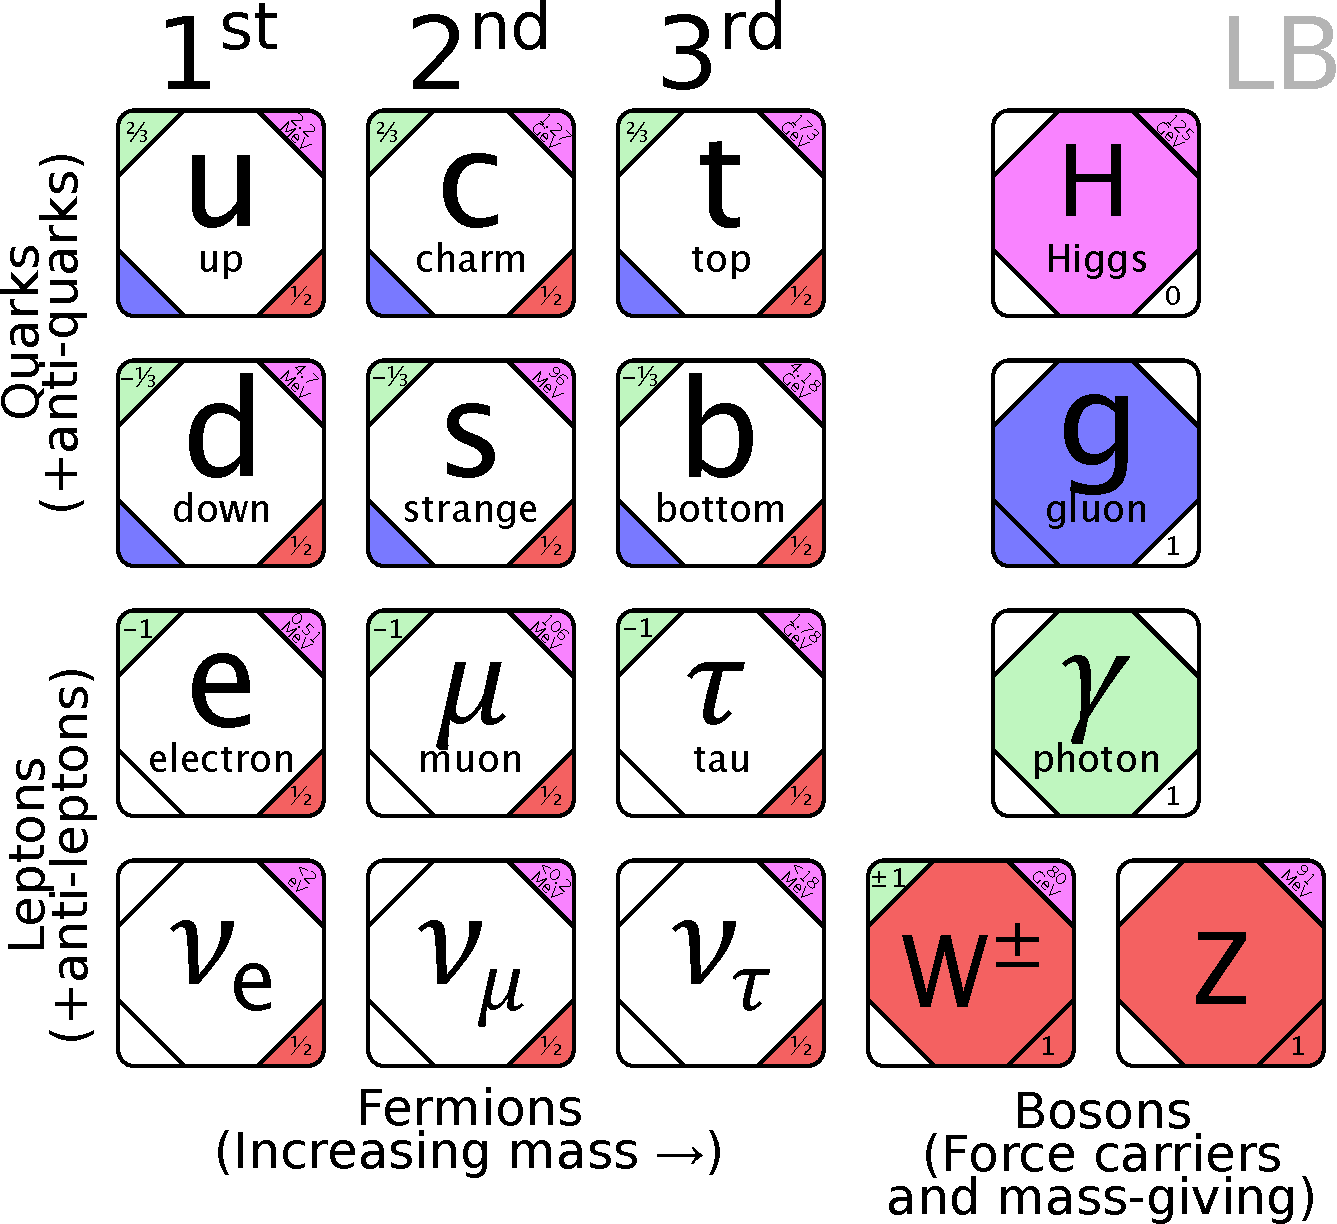
\includegraphics[width=\textwidth]{theory/SM}
    \caption{
        The various particles of the Standard~Model of particle~physics, with fermions on the left and bosons on the right.
        In each box several properties are denoted: electric~charge in the top-left~corner, mass in the top-right~corner, presence or absence of colour in the lower-left~corner, and weak~isospin in the lower-right~corner.}
    \label{fig:theory_SM_Particles}
\end{figure}
%
\begin{itemize}
    \item The electromagnetic force, mediated by the photon~(\g). This force acts upon any charged particle, including the six quarks, the three charged leptons, and the \Wpm~bosons.
    \item The weak force, mediated by the \Wpm~and \Z~bosons. This force acts upon isospin-charged particles, including all the fermions, and the \Wpm~and \Z~bosons themselves.
    \item The strong force, mediated by the gluons~(\gluon). This force acts upon colour-charged particles: the six quarks, as well as the gluons themselves.
\end{itemize}

The~SM describes both ordinary matter and its counterpart, antimatter.
Fundamentally, the theory requires that matter and corresponding antimatter particles have the same mass and lifetime.
Furthermore, electromagnetic and strong interactions are symmetric for matter and antimatter particles.
This symmetry is \CP~symmetry, where \CP~is defined as the successive application of two discrete symmetries: charge conjugation~\(C\) and the parity inversion~\(P\).
The \(C\)~operation transforms particles into antiparticles and vice versa, while the \(P\)~operation transforms \({\left(x, y, z\right)}\)~coordinates into~\({-\left(x, y, z\right)}\), and therefore interchanges left- and right-handed particles.

In the Standard~Model, parity violation is described by introducing a weak force gauge symmetry only for left-handed particles and right-handed antiparticles.
\CP~violation in the~SM, a subtle manifestation of which was discovered in~1964~\cite{CPinKaon}, is possible due to complex interaction couplings in the weak interaction.
The origin of this lies in the fact that the weak interaction eigenstates of the fermions are not identical to the mass eigenstates.

\clearpage
\section{The CKM~matrix}
\label{sec:CKM}

In the Standard Model Lagrangian, the mass terms of the quark fields arise from the Yukawa couplings between the quarks and the Higgs field,
%
\begin{equation}
    \Lagrangian_{\text{Yukawa}}^{\text{quarks}} = Y_{ij}^{d} \overline{Q_{\text{L},i}^{\text{I}}} \phi d_{\text{R},i}^{\text{I}} + Y_{ij}^{u} \overline{Q_{\text{L},i}^{\text{I}}} \tilde{\phi} u_{\text{R},i}^{\text{I}} \text{h.c.} \rlap{,}
\end{equation}
%
with the Yukawa~couplings~\(Y\) between the Higgs~doublets~\(\phi\) and~\(\tilde{\phi}\), the left-handed quark doublets~\(Q_{\text{L}}^{\text{I}}\), and the right-handed quark fields~\(d_{\text{R}}^{\text{I}}\) and~\(u_{\text{R}}^{\text{I}}\).
The label~I denotes expression in the interaction basis.
After spontaneous symmetry breaking~\cite{PhysRevLett.13.321,PhysRevLett.13.508}, the doublets are split, and the Yukawa couplings give rise to the quark mass terms,
%
\begin{equation}
    \Lagrangian_{\text{Yukawa}}^{\text{quarks}} = v Y_{ij}^{d} \overline{d_{\text{L},i}^{\text{I}}} d_{\text{R},i}^{\text{I}} + v Y_{ij}^{u} \overline{u_{\text{L},i}^{\text{I}}} u_{\text{R},i}^{\text{I}} + \text{h.c.} \rlap{,}
\end{equation}
%
where \({v = \SI{246}{\GeV}}\)~is the vacuum expectation value.
The interactions between the Higgs~boson and the quark fields have been omitted for brevity.

The Lagrangian of the charged-current interaction,
%
\begin{equation}
    \Lagrangian_{\text{cc}}^{\text{quarks}} = \dfrac{g}{\sqrt{2}} \left[ \overline{u_{\text{L},i}^{\text{I}}} \gamma_{\mu} \dfrac{1 - \gamma^{5}}{2} W^{-}{}^{\mu} d_{\text{L},i}^{\text{I}}
        + \overline{d_{\text{L},i}^{\text{I}}} \gamma_{\mu} \dfrac{1 - \gamma^{5}}{2}  W^{+}{}^{\mu} u_{\text{L},i}^{\text{I}} \right] \rlap{,}
\end{equation}
%
can be rewritten with the quark interaction fields in their mass eigenstates.
This requires diagonalisation of the matrix of Yukawa couplings, leading to
%
\begin{equation}
    \Lagrangian_{\text{cc}}^{\text{quarks}} = \dfrac{g}{\sqrt{2}} \left[
          \overline{u_{\text{L},i}} V_{\text{L}}^{u} \gamma_{\mu} \dfrac{1 - \gamma^{5}}{2} W^{-}{}^{\mu} V_{\text{L}}^{d}{}^{\dagger} d_{\text{L},i}
        + \overline{d_{\text{L},i}} V_{\text{L}}^{d} \gamma_{\mu} \dfrac{1 - \gamma^{5}}{2} W^{+}{}^{\mu} V_{\text{L}}^{u}{}^{\dagger} u_{\text{L},i}
    \right] \rlap{,}
\end{equation}
%
where the unitary matrices~\(V_{\text{L}}^{u}\) and~\(V_{\text{L}}^{d}\) diagonalise the matrix of up- and down-type quarks, respectively.

The interaction eigenstates can now be related to the mass eigenstates through the complex, unitary~\num{3x3} CKM~matrix~\({\VCKM = V_{\text{L}}^{u} V_{\text{L}}^{d}{}^{\dagger}}\), named after Cabibbo, Kobayashi and Maskawa,~\cite{CKM1,CKM2}
%
\begin{equation} \label{eqn:theory_CKM_Matrix}
    \begin{pmatrix}
        \dquark^{\text{I}} \\
        \squark^{\text{I}} \\
        \bquark^{\text{I}}
    \end{pmatrix}
    =
    \VCKM
    \begin{pmatrix}
        \dquark \\
        \squark \\
        \bquark
    \end{pmatrix}
    =
    \begin{pmatrix}
        \Vud & \Vus & \Vub \\
        \Vcd & \Vcs & \Vcb \\
        \Vtd & \Vts & \Vtb
    \end{pmatrix}
    \begin{pmatrix}
        \dquark \\
        \squark \\
        \bquark
    \end{pmatrix} \rlap{.}
\end{equation}
%
These nine complex numbers~\(\V{ij}\) define the relative values of the charged-current couplings in which a quark changes flavour.
The only interaction allowing flavour changes in the~SM is the weak interaction, through the charged \Wpm~bosons.
Under the \CP~transformation, each CKM~element changes into its complex conjugate, and thus it is the complex phases of the elements that can yield \CP~violation in the SM.

Since the CKM~elements only enter at the amplitude level, a single Feynman diagram can never yield measurable \CP~violation: the observable quantity, the magnitude of the amplitude, is then identical for the \CP-conjugate process.
Therefore, a prerequisite for observing \CP~violation is the interference between two amplitudes of comparable magnitude and with a different weak phase.
The complex phase of the weak interaction (known as the ``weak~phase'') will change sign under the \CP~transformation.
Measuring the difference in decay-rate between a process and its \CP-conjugate allows the determination of the phase difference between them, and hence of the weak phase difference and the amount of \CP~violation in that process.

To conserve total probability, the CKM~matrix must be unitary:~\({\VCKM\VCKMd = \VCKMd\VCKM = \identitymatrix}\).
This results in the following unitarity relations between the elements of the matrix:
%
\begin{subequations} \label{eqn:theory_CKM_Unitarity}
    \begin{align}
        \sum_{k} \V{ik} \Vs{jk} &= 0 \rlap{,} \label{eqn:theory_CKM_Unitarity_1} \\
        \sum_{k} \abs{\V{ik}}^{2} = \sum_{k} \abs{\V{ki}}^{2} &= 1 \rlap{,} \label{eqn:theory_CKM_Unitarity_2}
    \end{align}
\end{subequations}
%
for any two generations~\({i, j \in \{ u, c, t \}}\),~\({i \neq j}\).
From the original \num{18}~degrees of freedom of the matrix, these constraints leave a total of five relative quark field phases and four free parameters with which the matrix can be fully described: three angles and one complex phase.
Hence, the entirety of measurable \CP~violating phenomena in the~SM is reduced to a single parameter: the complex phase of the CKM~matrix.
It is noteworthy that this phase only appears in the case of at least three generations, making the~SM the minimal model with \CP~violation in the weak interaction.

The four parameters of the CKM~matrix are in principle free parameters of the Standard~Model, but they have been experimentally determined to show an interesting pattern.
The magnitudes of the diagonal elements are all close to unity, while the off-diagonal terms are smaller the greater the difference between the generations.
A common way of parameterising the matrix that exploits this structure is the Wolfenstein parameterisation~\cite{Wolfenstein:1983yz}.
This parameterisation consists of three real variables~\wolfl, \wolfA, and \wolfrho and one imaginary part \({i\wolfeta}\).
By construction, \({\wolfl = \sin(\theta_{\text{c}}) \approx 0.225}\)~\cite{CKM1}, naturally leading to an expansion in powers of~\wolfl.
Up to \({\order(\wolfl^{4})}\), the matrix takes the form
%
\begin{equation} \label{eqn:theory_CKM_Wolfenstein}
    \VCKM
    =
    \begin{pmatrix}
        1 - \frac{1}{2}\wolfl^{2} - \frac{1}{8}\wolfl^{4} & \wolfl & \wolfA\wolfl^{3}(\wolfrho - i\wolfeta) \\[.5ex]
        -\wolfl & 1 - \frac{1}{2}\wolfl^{2} - \frac{1}{8}\wolfl^{4}(1 + 4\wolfA^{2}) & \wolfA\wolfl^{2} \\[.5ex]
        \wolfA\wolfl^{3} (1 - \wolfrho - i\wolfeta) & -\wolfA\wolfl^{2} + \frac{1}{2}\wolfA\wolfl^{4}(1 - 2(\wolfrho + i\wolfeta)) & 1 - \frac{1}{2}\wolfA^{2}\wolfl^{4}
    \end{pmatrix} \rlap{.}
\end{equation}
%
Written in this form, the diagonal elements are recognised as a small deviation from unity, while the off-diagonal elements are all smaller with certain powers of~\wolfl.
The current world-average experimental determination of the parameters is~\cite{HFLAV2016}
%
\begin{subequations}
    \begin{align}
        \wolfl    &= {0.22543 }_{-0.00031}^{+0.00042} \\
        \wolfA    &= {0.8227\0}_{-0.0136}^{+0.0066} \\
        \wolfrhob &= {0.1504\0}_{-0.0062}^{+0.0121} \\
        \wolfetab &= {0.3540\0}_{-0.0076}^{+0.0069}
    \end{align}
\end{subequations}
%
where~\({\wolfrho + i\wolfeta}\) of \cref{eqn:theory_CKM_Wolfenstein} has been substituted by~\({\wolfrhob + i\wolfetab}\), defined as
%
\begin{equation} \label{eqn:theory_CKM_rhob_etab}
    \wolfrhob + i\wolfetab = -\dfrac{\Vud\Vubs}{\Vcd\Vcbs} = \dfrac{\sqrt{1-\wolfl^{2}} (\wolfrho + i\wolfeta)}{\sqrt{1 - \wolfA^{2}\wolfl^{4}} + \sqrt{1 - \wolfl^{2}}\wolfA^{2}\wolfl^{4}(\wolfrho + i\wolfeta)} \rlap{.}
\end{equation}

The six relations in \cref{eqn:theory_CKM_Unitarity_1} can be visualised as triangles in the complex plane, allowing verification of the compatibility of various measurements by checking that the triangles close.
The most pronounced unitarity triangle~(UT) is shown in \cref{fig:theory_CKM_UTBd}, with its apex at~\({\wolfrhob + i\wolfetab}\), justifying the definition in \cref{eqn:theory_CKM_rhob_etab}.
While the individual phases of the CKM~elements are not physical observables, certain combinations of phases are measurable quantities.
Those combinations show up in the UTs as the angles \CPalpha, \CPbeta, \CPgamma, and~\betas, as shown in \cref{fig:theory_CKM_UT}.
Additionally, the surface area of each UT is equal to \(\sfrac{1}{2}\)~the Jarlskog invariant~\Jarlskog,~\cite{PhysRevLett.55.1039}
%
\begin{equation} \label{eqn:theory_CKM_Jarlskog}
    \Jarlskog = \wolfl^{6}\wolfA^{2}\wolfeta \approx \num{3e-5}\rlap{.}
\end{equation}
%
The Jarlskog invariant is a measure of the amount of \CP~violation in the SM.

This thesis describes a measurement of~\weak, with \({\CPgamma = \arg\left(-\dfrac{\Vud\Vubs}{\Vcd\Vcbs}\right)}\) and~\({\betas = \arg\left(-\dfrac{\Vts\Vtbs}{\Vcs\Vcbs}\right)}\).
Using external input for~\betas from \BsToJPsiPhi~decays~\cite{HFLAV2016}, a determination of~\CPgamma is made, one the least-precise known observables constraining the apices of the UTs.
It should be noted that, in the Wolfenstein parameterisation up to~\({\order(\wolfl^{4})}\), \CPgamma~is given by the phase of~\Vub, \({\CPgamma \approx -\arg(\Vub)}\).

\begin{figure}[p] \centerfloat
    \begin{subfigure}{\textwidth} \centerfloat
        \begin{tikzpicture}
            \node[anchor=south west,inner sep=0] (image) at (0,0) {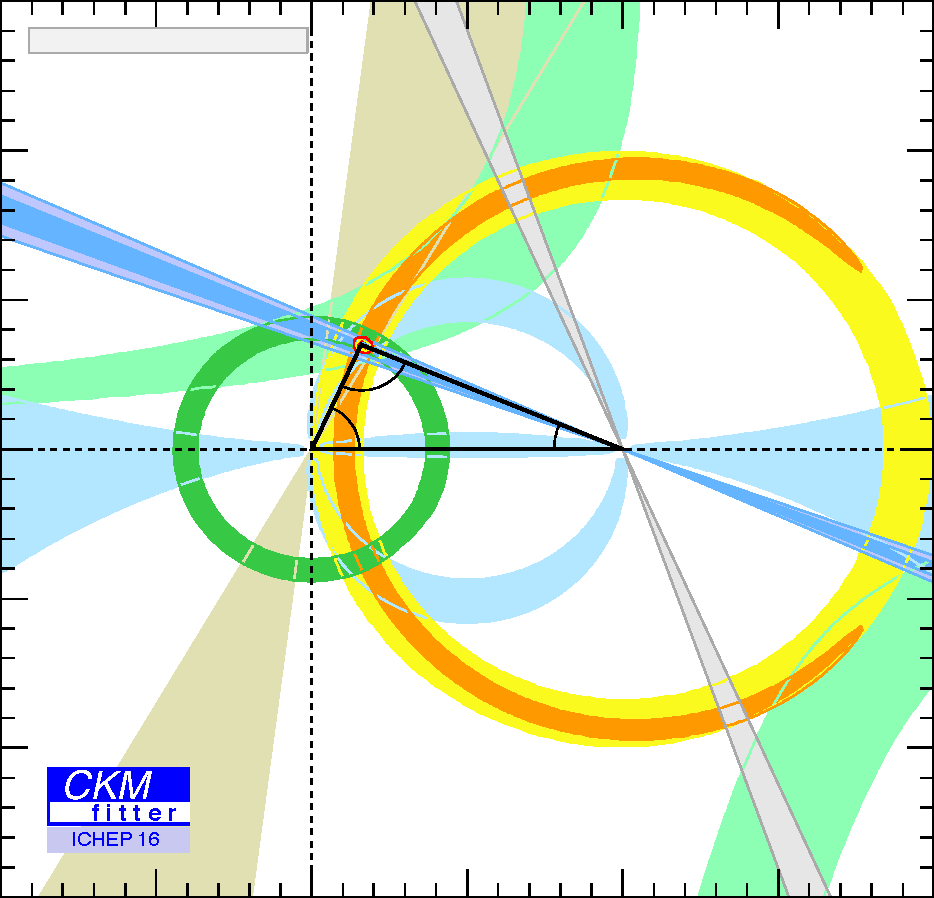
\includegraphics[width=0.55\textwidth]{theory/rhoeta_large}};
            \begin{scope}[x={(image.south east)},y={(image.north west)}]
                \node at (1. / 6. - 0.02, -0.027) {\(\pgfmathprintnumber[fixed,precision=1,fixed zerofill=true]{-0.5}\)};
                \foreach \x in {0, 2, 3, ..., 6}
                {
                    \tikzmath{\xpos = \x / 6.; \xtext = \x * 0.5 - 1.0;}
                    \node at (\xpos, -0.027) {\(\pgfmathprintnumber[fixed,precision=1,fixed zerofill=true]{\xtext}\)};
                }
                \node[anchor=east] at (0.005, 0.008) {\(\pgfmathprintnumber[fixed,precision=1,fixed zerofill=true]{-1.5}\)};
                \foreach \y in {1, ..., 6}
                {
                    \tikzmath{\ypos = \y / 6.; \ytext = \y * 0.5 - 1.5;}
                    \node[anchor=east] at (0.005, \ypos) {\(\pgfmathprintnumber[fixed,precision=1,fixed zerofill=true]{\ytext}\)};
                }

                {
                    \fontsize{4}{4.8}\selectfont
                    \node[anchor=west] at (0.04, 0.955) {excluded area has \({\text{CL} > \num{0.95}}\)};
                    \node[anchor=west,rotate=-68] at (0.475, 0.995) {excluded at \({\text{CL} > \num{0.95}}\)};
                    \node[anchor=west] at (0.76, 0.08) {sol. w/ \({\cos 2\CPbeta < 0}\)};
                    \node[anchor=west] at (0.76, 0.05) {(excl. at \({\text{CL} > \num{0.95}}\))};
                }
                {
                    \fontsize{10}{12}\selectfont
                    \node[anchor=west] at (0.40, 0.885) {\CPgamma};
                    \node[anchor=west] at (0.665, 0.810) {\dmd~\&~\dms};
                    \node[anchor=west] at (0.02, 0.730) {\({\sin 2\CPbeta}\)};
                    \node[anchor=west] at (0.82, 0.630) {\dmd};
                    \node[anchor=west] at (0.03, 0.575) {\epsK};
                }
                {
                    \fontsize{7}{8.4}\selectfont
                    \node[anchor=west] at (0.365, 0.580) {\CPalpha};
                    \node[anchor=west] at (0.530, 0.519) {\CPbeta};
                    \node[anchor=west] at (0.34, 0.514) {\CPgamma};
                }
                {
                    \fontsize{10}{12}\selectfont
                    \node[anchor=west] at (0.03, 0.460) {\CPalpha};
                    \node[anchor=west] at (0.175, 0.390) {\abs{\Vub}};
                    \node[anchor=west] at (0.59, 0.390) {\CPalpha};
                    \node[anchor=west] at (0.205, 0.165) {\CPgamma};
                    \node[anchor=west] at (0.86, 0.190) {\epsK};
                }

                \node[anchor=east] at (1.0, -0.10) {\wolfrhob};
                \node[rotate=90,anchor=east,inner xsep=0pt,outer xsep=0pt] at (-0.12, 1.0) {\wolfetab};
            \end{scope}
        \end{tikzpicture}
        \caption{The best-known Unitarity~Triangle, corresponding to \({\Vud\Vubs + \Vcd\Vcbs + \Vtd\Vtbs = 0}\). Its apex is at the point given in \cref{eqn:theory_CKM_rhob_etab}.}
        \label{fig:theory_CKM_UTBd}
    \end{subfigure}
    \begin{subfigure}{\textwidth} \centerfloat
        \begin{tikzpicture}
            \node[anchor=south west,inner sep=0] (image) at (0,0) {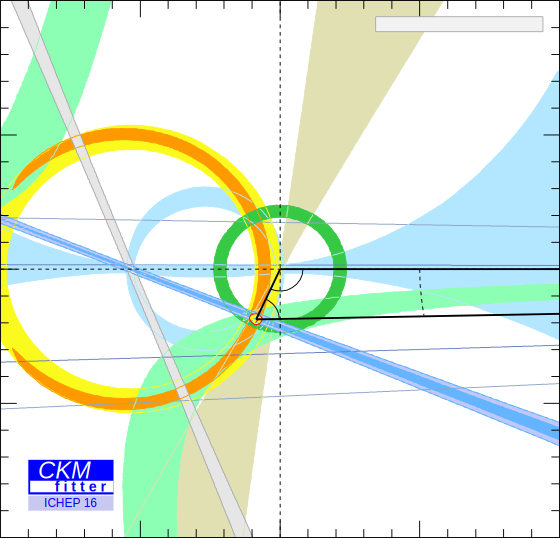
\includegraphics[width=0.55\textwidth]{theory/rhoetaBs_large}};
            \begin{scope}[x={(image.south east)},y={(image.north west)}]
                \node at (1. / 4. - 0.02, -0.027) {\(\pgfmathprintnumber[fixed,precision=1,fixed zerofill=true]{-0.05}\)};
                \foreach \x in {0, 2, 3, 4}
                {
                    \tikzmath{\xpos = \x / 4.; \xtext = \x * 0.05 - 0.10;}
                    \node at (\xpos, -0.027) {\(\pgfmathprintnumber[fixed,precision=2,fixed zerofill=true]{\xtext}\)};
                }
                \node[anchor=east] at (0.005, 0.010) {\(\pgfmathprintnumber[fixed,precision=2,fixed zerofill=true]{-0.10}\)};
                \foreach \y in {1, ..., 4}
                {
                    \tikzmath{\ypos = \y / 4.; \ytext = \y * 0.05 - 0.10;}
                    \node[anchor=east] at (0.005, \ypos) {\(\pgfmathprintnumber[fixed,precision=2,fixed zerofill=true]{\ytext}\)};
                }

                {
                    \fontsize{4}{4.8}\selectfont
                    \node[anchor=west] at (0.677, 0.955) {excluded area has \({\text{CL} > \num{0.95}}\)};
                    \node[anchor=west,rotate=-68] at (0.04, 0.995) {excluded at \({\text{CL} > \num{0.95}}\)};
                    \node[anchor=west] at (0.752, 0.465) {\betas};
                }
                {
                    \fontsize{10}{12}\selectfont
                    \node[anchor=west] at (0.090, 0.945) {\epsK};
                    \node[anchor=west] at (0.560, 0.925) {\CPgamma};
                    \node[anchor=west] at (0.180, 0.730) {\dmd~\&~\dms};
                    \node[anchor=west] at (0.010, 0.605) {\dmd};
                    \node[anchor=west] at (0.243, 0.590) {\CPalpha};
                    \node[anchor=west] at (0.504, 0.600) {\abs{\Vub}};
                    \node[anchor=west] at (0.868, 0.575) {\CPalpha};
                    \node[anchor=west] at (0.540, 0.255) {\betas};
                    \node[anchor=west] at (0.390, 0.200) {\CPgamma};
                    \node[anchor=west] at (0.829, 0.200) {\({\sin 2\CPbeta}\)};
                    \node[anchor=west] at (0.230, 0.103) {\epsK};
                }

                \node[anchor=east] at (1.0, -0.10) {\(\wolfrhob_{\squark\bquark}\)};
                \node[rotate=90,anchor=east,inner xsep=0pt,outer xsep=0pt] at (-0.16, 1.0) {\(\wolfetab_{\squark\bquark}\)};
            \end{scope}
        \end{tikzpicture}
        \caption{The Unitarity~Triangle for the \Bs~system, corresponding to \({\Vus\Vubs + \Vcs\Vcbs + \Vts\Vtbs = 0}\), with apex \(\wolfrhob_{\squark\bquark} + i\wolfetab_{\squark\bquark} = -\Vus\Vubs/\left(\Vcs\Vcds\right)\).}
        \label{fig:theory_CKM_UTBs}
    \end{subfigure}
    \caption{
        Two Unitarity Triangles.
        The various constraints on the apex of each of the triangles match, confirming the validity of the CKM~matrix.
        Figures adapted from Ref.~\cite{CKMFitter}.}
    \label{fig:theory_CKM_UT}
\end{figure}

\clearpage
\section{Weak hadronic beauty decays}
\label{sec:theory_WeakDecays}

Beauty hadrons, or hadrons containing a \bquark~quark, decay weakly with the transition of the \bquark~quark into a lighter quark through the charged-current couplings of the weak interaction.
The effects of the strong interaction, within (as well as between) the involved hadrons, are challenging to describe analytically.
Rather, an effective approach, using experimental input, is warranted.

\subsection{Decay topologies}
\label{sec:theory_tree_exchange}

In weak beauty hadron decays, several decay topologies can be identified, as illustrated in \cref{fig:theory_Topologies_Tree,fig:theory_Topologies_Exchange}.
Tree topologies are those in which the \Wpm~boson is emitted from the \bquark~hadron and the other quark(s) of the hadron are \emph{spectator}~quarks, that do not directly participate in the decay.
%
\begin{figure}[hb] \centerfloat
    \begin{tikzpicture}
        \newlength{\diagramsize}
        \setlength{\diagramsize}{3.5em}
        \newlength{\diagramheight}
        \setlength{\diagramheight}{\baselineskip}
        \begin{feynman}
            \vertex (a1);
            \vertex[right=2\diagramsize of a1] (a2);
            \vertex[right=2\diagramsize of a2] (a3) {\quark};

            \vertex[below=\diagramheight of a1] (b1);
            \vertex[right=2\diagramsize of b1] (b2);
            \vertex[right=2\diagramsize of b2] (b3) {\(\quark\prime\)};

            \vertex[below=\diagramheight of b1] (c1);
            \vertex[right=2\diagramsize of c1] (c2);
            \vertex[right=2\diagramsize of c2] (c3) {\(\quark\dprime\)};

            \vertex[above right=4\diagramheight and \diagramsize of a2] (x1);
            \vertex[above right=1.25\diagramheight and \diagramsize of x1] (x2);
            \vertex[below right=1.25\diagramheight and \diagramsize of x1] (x3);

            \diagram* {
                {[edges=fermion]
                    (a1) -- (a2) -- (a3),
                    (x1) -- (x2),
                    (x3) -- (x1),
                },
                (b1) -- (b3),
                (c1) -- [scalar] (c3),
                (a2) -- [boson, edge label=\(\W\)] (x1),
            };

            \node[at=(c1), anchor=mid east] (q2) {\(\quark\dprime\)};
            \node[at=(q2.mid |- b1), anchor=mid] (q1) {\(\quark\prime\)};
            \node[at=(q1.mid |- a1), anchor=mid] (b) {\bquark};

            \node[at=(x2), anchor=mid west] (m1) {\(\Pm_{1}\)};
            \node[at=(x3), anchor=mid west] (m2) {\(\Pm_{2}\)};

            \draw [decoration={brace}, decorate] (q2.south west) -- (q2.south west |- b.north west) node [midway, left] {\PB};
            \draw [decoration={brace}, decorate] (a3.north east -| c3.south east) -- (c3.south east) node [midway, right] {\PH};
            \draw [decoration={brace}, decorate] (c3.south east |- m1.north east) -- (c3.south east |- m2.south east) node [midway, right] {\PM};
        \end{feynman}
    \end{tikzpicture}
    \caption{
        Tree-level topology of a \bquark~hadron~\PB weakly decaying into a lighter hadron~\PH by ejecting a meson~\PM.
        The quarks~\({\quark\prime}\) (and~\({\quark\dprime}\) in the case \PB~is a~baryon) are spectator quarks that do not take part in the interaction.
        At the \Wpm~vertices, the CKM~elements~\V{\quark\bquark} and~\Vs{\Pm_{2}\Pm_{1}} play a role.}
    \label{fig:theory_Topologies_Tree}
\end{figure}

Because of the gluonic interactions between the quarks in such diagrams, analytically calculating the amplitude is unfeasible.
The amplitude of a tree diagram can however be effectively described using only two factorised components: strong interactions in the decay of the \bquark~hadron, and those in the production of the separate hadron at the other end of the \Wpm~boson.
The former of these is described by the form factor~\(F\), which is different for each combination of two hadrons.
The form factor is a function of the transferred momentum~\(q^{2}\) of the system, with, in the case of hadronic decays,~\({q^{2} = m_{\PM}^{2}}\).
The latter is covered by the decay constant~\(f\), with a hadron-specific (but otherwise constant) value.
Both can be determined using (semi)leptonic decays, such as~\BdDmunu for~\(F_{\decay{\Bd}{\Dm}}\) and~\decay{\Dsp}{\mup\neum} for~\(f_{\Dspm}\).

In the factorisation approximation, these two contributions fully describe the amplitude.
However, in practice, Feynman~diagrams in which gluons are exchanged between the two final-state hadrons can also play a role~\cite{Beneke:2000ry}.
Such diagrams add nonfactorisable effects in the form of a factor~\aNF.
Since~\aNF depends on the decay under study as well as on~\(q^{2}\) in the decay, constraining its value can be involved.

Taking into account CKM~factors, the expression for a decay of the form~\(\decay{\PB}{\PH\PM}\) (following the notation of \cref{fig:theory_Topologies_Tree}) becomes
%
\begin{equation} \label{eqn:theory_BF}
    \BF(\decay{\PB}{\PH\PM}) \propto \abs{\V{\quark\bquark}}^{2} \abs{\V{\Pm_{2}\Pm_{1}}}^{2} \abs{F_{\decay{\PB}{\PH}}}^{2} f_{\PM}^{2} \abs{\aNF}^{2} \rlap{,}
\end{equation}
%
where the proportionality indicates that several well-known phase-space factors are omitted for brevity.
Assuming the CKM~element~\V{\Pm_{2}\Pm_{1}} and the decay constant~\(f_{\PM}\) are known, the branching fraction can thus be used to study a combination of the CKM~element~\V{\quark\bquark} (where \({\quark \in \{\uquark, \cquark}\)), the form factor~\(F_{\decay{\PB}{\PH}}\), and the nonfactorisation of the particular decay.

Tree topologies are relatively well-understood, and measuring tree-level processes are used in measurements of \CP~violation, or the magnitude of the CKM~element~\Vub using \decay{\bquark}{\uquark}~decays.
However, additional decay topologies with a relative weak phase can contribute to the measured \CP~violation.
It is thus important to understand the various possible decay topologies, including:
%
\begin{description}
    \item[Exchange topologies (\cref{fig:theory_Topologies_Exchange}).] Topologies where a \Wpm~boson is exchanged between the two initial quarks, elaborated below.
    \item[Penguin topologies (\cref{fig:theory_Topologies_Penguin}).] These have a loop producing two of the four final-state quarks, either through a gluon or via an electroweak interaction.
    \item[Colour-suppressed topologies (\cref{fig:theory_Topologies_ColourSuppressed}).] These are similar to tree topologies, but the meson~\(M\) is internal, limiting the colour configurations available and suppressing the amplitude.
    \item[Annihilation topologies (\cref{fig:theory_Topologies_Annihilation}).] Here, the quarks in a charged meson directly annihilate into a \Wpm~boson.
    \item[Penguin annihilation topologies (\cref{fig:theory_Topologies_PenguinAnnihilation}).] A combination of the former two, the annihilation can also proceed through a penguin loop.
\end{description}
%
\begin{figure}[htb] \centerfloat
    \setlength{\diagramsize}{5em}
    \setlength{\diagramheight}{1.5\baselineskip}
    \begin{tikzpicture}
        \begin{feynman}
            \vertex (a1) {\bquark};
            \vertex[right=\diagramsize of a1] (a2);

            \vertex[below=2\diagramheight of a1] (b1) {\quark};
            \vertex[right=\diagramsize of b1] (b2);

            \vertex[above right=3\diagramheight and \diagramsize of a2] (x1);
            \vertex[below=2\diagramheight of x1] (x2);
            \vertex[below right= \diagramheight and \diagramheight of a2] (c);
            \vertex[below right=3\diagramheight and \diagramsize of b2] (x4);
            \vertex[above=2\diagramheight of x4] (x3);

            \diagram* {
                {[edges=fermion]
                    (a1) -- (a2),
                    (b2) -- (b1),
                    (a2) -- (x1),
                    (x2) -- (c) ,
                    (c)  -- (x3),
                    (x4) -- (b2),
                },
                (a2) -- [boson, edge label'=\(\W\)] (b2),
            };

            \node[at=(x1), anchor=mid west] (m1) {\(\Pm_{1}\)};
            \node[at=(x2), anchor=mid west] (m2) {\(\Pm_{2}\)};
            \node[at=(x4), anchor=mid west] (n1) {\(\Pn_{1}\)};
            \node[at=(x3), anchor=mid west] (n2) {\(\Pn_{2}\)};

            \draw [decoration={brace}, decorate] (b1.south west) -- (b1.south west |- a1.north west) node [midway, left] {\PB};
            \draw [decoration={brace}, decorate] (m1.north east) -- (m1.north east |- m2.south east) node [midway, right] {\PM};
            \draw [decoration={brace}, decorate] (n2.north east) -- (n2.north east |- n1.south east) node [midway, right] {\PN};
        \end{feynman}
    \end{tikzpicture}
    \caption{
        Generic form of an exchange topology of a meson~\PB decaying into two mesons~\PM and~\PN, with a \W~boson being exchanged between the two quarks of~\PB.
        Note that the quarks~\(\Pm_{2}\) and~\(\Pn_{2}\) originate from a gluon in the sea, and are necessarily of the same flavour.}
    \label{fig:theory_Topologies_Exchange}
\end{figure}
%
\begin{figure}[hb] \centerfloat
    \begin{tikzpicture}
        \setlength{\diagramsize}{3.5em}
        \setlength{\diagramheight}{2\baselineskip}
        \begin{feynman}
            \vertex (a1);
            \vertex[right=2\diagramsize of a1] (a2);
            \vertex[right=2\diagramsize of a2] (a3);
            \vertex[right=2\diagramsize of a3] (a4) {\quark};

            \vertex[below=\diagramheight of a1] (b1);
            \vertex[right=2\diagramsize of b1] (b2);
            \vertex[right=2\diagramsize of b2] (b3);
            \vertex[right=2\diagramsize of b3] (b4) {\(\quark\prime\)};

            %30 degree angle
            \vertex[above right=.5\diagramsize and 1.866\diagramsize of a2] (z);

            \vertex[above right=3\diagramheight and \diagramsize of a3] (x1);
            \vertex[above right=.75\diagramheight and \diagramsize of x1] (x2);
            \vertex[below right=.75\diagramheight and \diagramsize of x1] (x3);

            \diagram* {
                {[edges=fermion]
                    (a1) -- (a2),
                    (a2) -- [edge label={\uquark, \cquark, \tquark}] (a3),
                    (a3) -- (a4),
                    (b4) -- (b1),
                    (x1) -- (x2),
                    (x3) -- (x1),
                },
                (a2) -- [boson, half left, edge label=\(\W\)] (a3),
                (z) -- [boson, edge label={\g, \Z}] (x1),
            };

            \node[at=(b1), anchor=mid east] (q1) {\(\quark\prime\)};
            \node[at=(q1.mid |- a1), anchor=mid] (b) {\bquark};

            \node[at=(x2), anchor=mid west] (m1) {\(\Pm_{1}\)};
            \node[at=(x3), anchor=mid west] (m2) {\(\Pm_{2}\)};

            \draw [decoration={brace}, decorate] (q1.south west) -- (q1.south west |- b.north west) node [midway, left] {\PB};
            \draw [decoration={brace}, decorate] (a4.north east -| m2.south east) -- (b4.south east -| m2.south east) node [midway, right] {\PH};
            \draw [decoration={brace}, decorate] (m1.north east) -- (m2.south east) node [midway, right] {\PM};
        \end{feynman}
    \end{tikzpicture}
    \caption{
        Example of an electroweak penguin topology.
        Another possibility is a QCD~penguin topology, where the the photon or \Z~boson is replaced by a colour-neutral gluon structure emitted from the quark in the loop.
        In either case, the quarks~\(\Pm_{1}\) and~\(\Pm_{2}\) are necessarily of the same flavour, as both the neutral currents and the strong interaction are flavour-conserving.}
    \label{fig:theory_Topologies_Penguin}
\end{figure}
%
The last of these plays a role in the decay~\BsDsK and is characterised by the exchange of the \Wpm~boson between the two quarks of the decaying meson, as shown in \cref{fig:theory_Topologies_Exchange}.
These tend to be suppressed compared to tree decays, due to colour-suppression from the internal vertex~\({(\Pm_{2}, \Pn_{2})}\).
This same vertex also requires two of the final-state quarks to be of the same flavour, restricting the decays in which this type of diagram plays a role.
One example where it occurs is the process~\BdDsK, which is studied in more detail in \cref{chp:DsK_BF} as a means to quantify the relative size of exchange topologies in general.
%
\begin{figure}[hp] \centerfloat
    \begin{subfigure}{\textwidth} \centerfloat
        \setlength{\diagramsize}{3em}
        \setlength{\diagramheight}{1.5\baselineskip}
        \begin{tikzpicture}
            \begin{feynman}
                \vertex (a1);
                \vertex[right=2\diagramsize of a1] (a2);
                \vertex[right=1.5\diagramsize of a2] (a3);
                \vertex[above right=\diagramheight and 1.5\diagramsize of a3] (a4) {\quark};

                \vertex[below=\diagramheight of a1] (b1);
                \vertex[right=2\diagramsize of b1] (b2);
                \vertex[below right=2\diagramheight and 3\diagramsize of b2] (b3) {\(\quark\prime\)};

                \vertex[below=\diagramheight of b1] (c1);
                \vertex[right=2\diagramsize of c1] (c2);
                \vertex[below right=2\diagramheight and 3\diagramsize of c2] (c3) {\(\quark\dprime\)};

                \vertex[below=\diagramheight of a3] (x1);
                \vertex[above right=\diagramheight and 1.5\diagramsize of x1] (x2);
                \vertex[below right=\diagramheight and 1.5\diagramsize of x1] (x3);

                \diagram* {
                    {[edges=fermion]
                        (a1) -- (a2) -- (a3) -- (a4),
                        (x2) -- (x1),
                        (x1) -- (x3),
                    },
                    (b1) -- (b2) -- (b3),
                    (c1) -- [scalar] (c2) -- [scalar] (c3),
                    (a2) -- [boson, edge label'=\(\W\)] (x1),
                };

                \node[at=(c1), anchor=mid east] (q2) {\(\quark\dprime\)};
                \node[at=(q2.mid |- b1), anchor=mid] (q1) {\(\quark\prime\)};
                \node[at=(q1.mid |- a1), anchor=mid] (b) {\bquark};

                \node[at=(x2), anchor=mid west] (m1) {\(\Pm_{1}\)};
                \node[at=(x3), anchor=mid west] (m2) {\(\Pm_{2}\)};

                \draw [decoration={brace}, decorate] (q2.south west) -- (q2.south west |- b.north west) node [midway, left] {\PB};
                \draw [decoration={brace}, decorate] (m2.north east) -- (m2.north east |- c3.south east)  node [midway, right] {\PH};
                \draw [decoration={brace}, decorate] (m1.south east |- a4.north east) -- (m1.south east) node [midway, right] {\PM};
            \end{feynman}
        \end{tikzpicture}
        \caption{
            Generic form of a colour-suppressed tree topology, with a \bquark~hadron~\PB decaying into a hadron~\PH and a meson~\PM.}
        \label{fig:theory_Topologies_ColourSuppressed}
    \end{subfigure}
    \\[4ex]
    \begin{subfigure}{\textwidth} \centerfloat
        \setlength{\diagramsize}{3em}
        \setlength{\diagramheight}{1.5\baselineskip}
        \begin{tikzpicture}
            \begin{feynman}
                \vertex (a1) {\bquark};
                \vertex[right=\diagramsize of a1] (a2);

                \vertex[below=2\diagramheight of a1] (b1) {\quark};
                \vertex[right=\diagramsize of b1] (b2);

                \vertex[below right=\diagramheight and \diagramheight of a2] (c1);
                \vertex[right=2\diagramsize of c1] (c2);
                \vertex[right=\diagramheight of c2] (c3);

                \vertex[above right=1.5\diagramsize and 1.5\diagramsize of c2] (x1);
                \vertex[below=\diagramheight of x1] (x2);
                \vertex[below right=1.5\diagramsize and 1.5\diagramsize of c2] (x4);
                \vertex[above=\diagramheight of x4] (x3);

                \diagram* {
                    (a1) -- [fermion] (a2),
                    (a2) -- [fermion] (c1),
                    (c1) -- [fermion] (b2),
                    (b2) -- [fermion] (b1),

                    (c2) -- [fermion] (x1),
                    (x2) -- [fermion] (c3),
                    (c3) -- [fermion] (x3),
                    (x4) -- [fermion] (c2),
                    (c1) -- [boson, edge label={\W}] (c2),
                };

                \node[at=(x1), anchor=mid west] (m1) {\(\Pm_{1}\)};
                \node[at=(x2), anchor=mid west] (m2) {\(\Pm_{2}\)};
                \node[at=(x4), anchor=mid west] (n1) {\(\Pn_{1}\)};
                \node[at=(x3), anchor=mid west] (n2) {\(\Pn_{2}\)};

                \draw [decoration={brace}, decorate] (b1.south west) -- (b1.south west |- a1.north west) node [midway, left] {\PB};
                \draw [decoration={brace}, decorate] (m1.north east) -- (m1.north east |- m2.south east) node [midway, right] {\PM};
                \draw [decoration={brace}, decorate] (n2.north east) -- (n2.north east |- n1.south east) node [midway, right] {\PN};
            \end{feynman}
        \end{tikzpicture}
        \caption{
            Annihilation topology, where a meson decays directly through a \Wpm~boson into two lighter mesons.}
        \label{fig:theory_Topologies_Annihilation}
    \end{subfigure}
    \\[4ex]
    \begin{subfigure}{\textwidth} \centerfloat
        \setlength{\diagramsize}{3em}
        \setlength{\diagramheight}{1.5\baselineskip}
        \begin{tikzpicture}
            \begin{feynman}
                \vertex (a1) {\bquark};
                \vertex[right=\diagramsize of a1] (a2);

                \vertex[below=2\diagramheight of a1] (b1) {\quark};
                \vertex[right=\diagramsize of b1] (b2);

                \vertex[below right=\diagramheight and \diagramheight of a2] (c1);
                \vertex[right=2\diagramsize of c1] (c2);
                \vertex[right=\diagramheight of c2] (c3);

                \vertex[above right=1.5\diagramsize and 1.5\diagramsize of c2] (x1);
                \vertex[below=\diagramheight of x1] (x2);
                \vertex[below right=1.5\diagramsize and 1.5\diagramsize of c2] (x4);
                \vertex[above=\diagramheight of x4] (x3);

                \diagram* {
                    (a1) -- [fermion] (a2),
                    (a2) -- [fermion, edge label={\uquark, \cquark, \tquark}] (c1),
                    (c1) -- [fermion, edge label={\uquark, \cquark, \tquark}] (b2),
                    (b2) -- [fermion] (b1),

                    (c2) -- [fermion] (x1),
                    (x2) -- [fermion] (c3),
                    (c3) -- [fermion] (x3),
                    (x4) -- [fermion] (c2),
                    (a2) -- [boson, edge label'={\W}] (b2),
                    (c1) -- [boson, edge label={\g, \Z}] (c2),
                };

                \node[at=(x1), anchor=mid west] (m1) {\(\Pm_{1}\)};
                \node[at=(x2), anchor=mid west] (m2) {\(\Pm_{2}\)};
                \node[at=(x4), anchor=mid west] (n1) {\(\Pn_{1}\)};
                \node[at=(x3), anchor=mid west] (n2) {\(\Pn_{2}\)};

                \draw [decoration={brace}, decorate] (b1.south west) -- (b1.south west |- a1.north west) node [midway, left] {\PB};
                \draw [decoration={brace}, decorate] (m1.north east) -- (m1.north east |- m2.south east) node [midway, right] {\PM};
                \draw [decoration={brace}, decorate] (n2.north east) -- (n2.north east |- n1.south east) node [midway, right] {\PN};
            \end{feynman}
        \end{tikzpicture}
        \caption{
            Penguin annihilation topology, a variant of the annihilation topology with a penguin loop at the left-hand side of the diagram.}
        \label{fig:theory_Topologies_PenguinAnnihilation}
    \end{subfigure}
    \caption{Various decay topologies discussed in the text.}
\end{figure}

\clearpage
\subsection{Factorisation}

Of the quantities entering in \cref{eqn:theory_BF}, most are understood and can be measured independent of the others.
The one for which this is not the case, is the nonfactorisation parameter~\aNF.
This parameter describes \eg~gluonic interaction between the final-state hadrons in a hadronic decay.
While the form factors and decay constants describe strong interactions within hadrons, and as such can be determined from (semi)leptonic decays, the nonfactorisable component only occurs in decays with multiple hadrons in the final state, and as such can not be determined independently.
An additional complication is the fact that it depends on the kinematics of the decay, making it delicate to transfer from one decay process to another.

For decays where the meson~\PM (see \cref{fig:theory_Topologies_Tree}) is light (\ie, a pion or kaon), results show that factorisation is compatible with unity up to a precision of about~\SI{5}{\percent}~\cite{Fleischer:2010ca}.
However, if the meson is heavier (\ie, a \DorDspm~meson), the contribution of nonfactorisable effects may be larger.
The unknown nonfactorisable effects in \ie \BdDsPi~(\({\PM = \Dsp}\), \({\PH = \pim}\))~decays prevent a clean determination of~\abs{\Vub} from the branching fraction measurement of that process (see \cref{chp:Vub}).
One way to probe the nonfactorisable effects in decays with a heavy meson emerging from the \Wpm~boson, is by comparing the decay widths of several processes of the form~\BDD~\cite{Bel:2015wha}, where \PB~is any \bquark~meson and each \PD~is a charmed meson.

Since the nonfactorisable component depends on the decay, this can not be directly translated to a numerical value for decays where one of the \DorDspm~mesons is replaced by a lighter hadron such as a pion, kaon or proton.
However, studying \BDD~decays still provides information on nonfactorisation in general, in particular an addition to current knowledge when both decay products are light.

Any decay topology, as introduced in the previous \lcnamecref{sec:theory_tree_exchange}, contributes to the branching fraction, and complicates the determination of the size of nonfactorisable effects in the tree decay.
Which topologies contribute depends on the quark configuration of the decay, which makes it possible to disentangle these contributions by studying ratios of particular decays.

One such ratio is that between hadronic and semileptonic decay widths, which takes the form~\cite{Bel:2015wha}
%
\begin{align}
    \tilde{R}_{\Dm} &= \dfrac{\Gamma(\BdDDs)}{[\deriv\Gamma(\BdDlnu)/\deriv q^{2}]|_{q^{2}=m_{\Dspm}^{2}}} \\
                 &= 6 \pi^{2} \abs{\Vcs}^{2} f_{\Dspm}^{2} X_{\Bd\Dpm}^{\Dspm} \abs{\aNFt^{\prime}}^{2} \left(1 + 2 \varepsilon \tilde{a}^{\prime} \cos \tilde{\theta}^{\prime} \cos{\CPgamma} + \varepsilon^{2} \tilde{a}^{\prime 2}\right) \rlap{,}
\end{align}
%
where \(X\)~represents a combination of the form factor and phase-space factors, and the terms at the end are corrections for penguin topologies: \(\tilde{a}^{\prime}\)~and \(\tilde{\theta}^{\prime}\)~are the magnitude and phase of those topologies, respectively, and
%
\begin{equation*}
    {\varepsilon = \frac{\wolfl^{2}}{1 - \wolfl^{2}} \approx \num{0.05}}
\end{equation*}
%
is a correction for the CKM~elements entering those topologies.
By inserting the experimentally known values, the combination of~\(\abs{\aNFt^{\prime}}\) and penguin contributions is found to be sizeable, at about~\SI{25}{\percent}~\cite{Bel:2015wha}.
The contribution of penguin topologies to that number can be determined from ratios of other \BDD~decays, including~\BsDsDs, \BsDD, and~\BdDDs, to be at least of the order~\SI{5}{\percent}.
More data is needed to further investigate the relative contributions of nonfactorisation and penguin topologies, in particular concerning the semileptonic decay rate~\BsDslnu.
However, this result already indicates that nonfactorisable effects in decays with heavy mesons can not be neglected.
This type of decays is studied further in \cref{chp:Vub}.

\clearpage
\section{\CP~violation}
\label{sec:theory_CPV}

\subsection{Mixing of neutral mesons}
\label{sec:theory_Mixing}

\begin{figure}[b] \centerfloat
    \begin{tikzpicture}
        \newlength{\mixingdiagramsize}
        \setlength{\mixingdiagramsize}{3.5em}
        \begin{feynman}
            \vertex (a1) {\bquark};
            \vertex[right=\mixingdiagramsize of a1] (a2);
            \vertex[right=\mixingdiagramsize of a2] (a3);
            \vertex[right=\mixingdiagramsize of a3] (a4) {\squark};

            \vertex[below=\mixingdiagramsize of a1] (b1) {\squark};
            \vertex[right=\mixingdiagramsize of b1] (b2);
            \vertex[right=\mixingdiagramsize of b2] (b3);
            \vertex[right=\mixingdiagramsize of b3] (b4) {\bquark};

            \diagram* {
                {[edges=fermion]
                    (b1) -- (b2) -- [edge label=\({\uquark, \cquark, \tquark}\)] (a2) -- (a1),
                    (a4) -- (a3) -- [edge label=\({\uquark, \cquark, \tquark}\)] (b3) -- (b4),
                },
                (a2) -- [boson, edge label=\(\W\)] (a3),
                (b2) -- [boson, edge label'=\(\W\)] (b3),
            };

            \draw [decoration={brace}, decorate] (b1.south west) -- (a1.north west) node [midway, left] {\Bs};
            \draw [decoration={brace}, decorate] (a4.north east) -- (b4.south east) node [midway, right] {\Bsb};
        \end{feynman}
        \begin{feynman}
            \vertex[right=6em of a4] (a1) {\bquark};
            \vertex[right=\mixingdiagramsize of a1] (a2);
            \vertex[right=\mixingdiagramsize of a2] (a3);
            \vertex[right=\mixingdiagramsize of a3] (a4) {\squark};

            \vertex[below=\mixingdiagramsize of a1] (b1) {\squark};
            \vertex[right=\mixingdiagramsize of b1] (b2);
            \vertex[right=\mixingdiagramsize of b2] (b3);
            \vertex[right=\mixingdiagramsize of b3] (b4) {\bquark};

            \diagram* {
                {[edges=fermion]
                    (b1) -- (b2) -- [edge label'=\({\uquark, \cquark, \tquark}\)] (b3) -- (b4),
                    (a4) -- (a3) -- [edge label'=\({\uquark, \cquark, \tquark}\)] (a2) -- (a1),
                },
                (a2) -- [boson, edge label'=\(\W\)] (b2),
                (a3) -- [boson, edge label=\(\W\)] (b3),
            };

            \draw [decoration={brace}, decorate] (b1.south west) -- (a1.north west) node [midway, left] {\Bs};
            \draw [decoration={brace}, decorate] (a4.north east) -- (b4.south east) node [midway, right] {\Bsb};
        \end{feynman}
    \end{tikzpicture}
    \caption{
        Feynman ``box''~diagrams involved in \Bs~meson mixing.
        The reverse diagrams are also possible, giving rise to the oscillation.
        The diagrams for \Kz,~\Dz,~and~\Bd~meson mixing are similar, except the \bquark~and \squark~quarks (as well as the \({\uquark, \cquark, \tquark}\)~quarks for the \Dz~meson) are replaced by other flavours.}
    \label{fig:theory_Mixing}
\end{figure}
%
Neutral mesons have the unique property that they can oscillate, periodically changing into their own antiparticle and back.
This so-called \emph{mixing} proceeds through two sets of similar Feynman~diagrams, depicted in \cref{fig:theory_Mixing}.
In certain decays, mixing provides the interfering diagrams required for measuring \CP~violation (see \cref{sec:CKM}).
The goal of this~\lcnamecref{sec:theory_Mixing} is to present a mathematical framework describing this time-dependent mixing for a neutral meson~\PP.

In general, the two flavour eigenstates of the meson can be written as~\ket{\pz} and~\ket{\pzb}. Over time, it will oscillate and become a superposition of both states. This is reflected in its wave-function,
%
\begin{equation}
    \psi(t) = a(t)\ket{\pz} + b(t)\ket{\pzb} = \begin{pmatrix} a(t) \tabularnewline b(t) \end{pmatrix}\rlap{,}
\end{equation}
%
where the last expression is written in the \({(\ket{\pz}, \ket{\pzb})}\)-basis.
In this basis, the Hamiltonian describing the mixing and decay of the system can be written as
%
\begin{equation} \label{eqn:theory_Mixing_Hamiltonian}
    \hat{H} = \mathbf{M} - \dfrac{i}{2} \upGamma\rlap{,}
\end{equation}
%
where the real part~\(\mathbf{M}\) describes the mixing and the imaginary part~\(\upGamma\) the decay of the meson (both are complex \num{2x2}~matrices).
Inserting both equations into the Schrödinger~equation yields
%
\begin{equation}
    i \dfrac{\partial\psi}{\partial t} = \hat{H} \psi = (\mathbf{M} - \dfrac{i}{2} \upGamma) \psi =
        \begin{pmatrix}
            M_{11} - \frac{i}{2} \Gamma_{11} & M_{12} - \frac{i}{2} \Gamma_{12} \tabularnewline[1ex]
            M_{21} - \frac{i}{2} \Gamma_{21} & M_{22} - \frac{i}{2} \Gamma_{22}
        \end{pmatrix} \psi\rlap{.}
\end{equation}
%
Under the assumption that \CPT~invariance holds, \({M_{11} = M_{22} = M}\), \({M_{21} = M_{12}^{\ast}}\), \({\Gamma_{11} = \Gamma_{22} = \Gamma}\), and~\({\Gamma_{21} = \Gamma_{12}^{\ast}}\), leading to
%
\begin{equation} \label{eqn:Theory_Mixing_TimeDepHamiltonian}
    i \dfrac{\partial\psi}{\partial t} =
        \begin{pmatrix}
            M - \frac{i}{2} \Gamma & M_{12} - \frac{i}{2} \Gamma_{12} \tabularnewline[1ex]
            M_{12}^{\ast} - \frac{i}{2} \Gamma_{12}^{\ast} & M - \frac{i}{2} \Gamma
        \end{pmatrix}\rlap{.}
\end{equation}

The eigenvectors of this Hamiltonian are the mass eigenstates of the meson system.
The heavier one is expressed as~\ket{\ph} and the lighter one as~\ket{\pl}:
%
\begin{subequations} \label{eqn:Theory_Mixing_PHPL}
    \begin{align}
        \ket{\ph} &= p\ket{\pz} - q\ket{\pzb} \rlap{,} \\
        \ket{\pl} &= p\ket{\pz} + q\ket{\pzb} \rlap{,}
    \end{align}
\end{subequations}
%
where \({(p, q)}\)~is the eigenvector (in \({(\pz, \pzb)}\) space) of the Hamiltonian of \cref{eqn:Theory_Mixing_TimeDepHamiltonian}.
The inverse of this equation is
%
\begin{subequations} \label{eqn:Theory_Mixing_PZPZB}
    \begin{align}
        \ket{\pz}  &= \dfrac{1}{2p} (\ket{\pl} + \ket{\ph}) \rlap{,} \\
        \ket{\pzb} &= \dfrac{1}{2q} (\ket{\pl} - \ket{\ph}) \rlap{.}
    \end{align}
\end{subequations}
%
Including the usual time evolution, \({\ket{\psi(t)} = e^{-iHt} \ket{\psi(0)}}\), \cref{eqn:Theory_Mixing_PHPL} becomes
%
\begin{subequations} \label{eqn:Theory_Mixing_PHPL_TimeDep}
    \begin{align}
        \ket{\ph(t)} &= e^{-i \mH t - \frac{1}{2} \GH t} \ket{\ph(0)} \rlap{,} \\
        \ket{\pl(t)} &= e^{-i \mL t - \frac{1}{2} \GL t} \ket{\pl(0)} \rlap{,}
    \end{align}
\end{subequations}
%
where~\mH and~\mL are the masses and~\GH and~\GL the decay widths of the mass~eigenstates.
Here, the choice of the factor~\(\frac{1}{2}\) in \cref{eqn:theory_Mixing_Hamiltonian} leads to \GH~and \GL~taking the usual definition of decay width.

The differences in mass and decay width between the two mass eigenstates are defined as
%
\begin{subequations}
    \begin{align}
        \dm &= \mH - \mL \rlap{,} \\
        \DG &= \GL - \GH \rlap{.}
    \end{align}
\end{subequations}
%
It should be noted here that while the sign of~\dm is fixed to be positive, the sign of~\DG must be verified experimentally\footnote{
    The apparent inconsistency in definitions between~\dm and~\DG is a convention in which both parameters are positive for the \Bs~system, as determined by experiments.
    This is the convention adapted by \hflav~\cite{HFLAV2016} and is used throughout this thesis.}.
These definitions, together with \cref{eqn:Theory_Mixing_PZPZB,eqn:Theory_Mixing_PHPL_TimeDep}, lead to an expression of the time-dependent mixing amplitude of a neutral meson, starting as either~\ket{\pz} or~\ket{\pzb}:
%
\begin{subequations} \label{eqn:Theory_Mixing_TimeDepMixingAmpl}
    \begin{align}
        \ket{\pz(t)}  = g_{+}(t) \ket{\pz}  &+ \left(\dfrac{q}{p}\right) g_{-}(t) \ket{\pzb} \rlap{,} \\
        \ket{\pzb(t)} = g_{+}(t) \ket{\pzb} &+ \left(\dfrac{p}{q}\right) g_{-}(t) \ket{\pz}  \rlap{,}
    \end{align}
\end{subequations}
%
where
%
\begin{equation} \label{eqn:Theory_Mixing_TimeDepMixingAmplG}
    g_{\pm}(t) = \dfrac{1}{2} e^{-i \frac{1}{2} (\mH + \mL) t} \left( e^{-i \frac{1}{2} \dm t - \frac{1}{2} \GH t} \pm e^{i \frac{1}{2} \dm t - \frac{1}{2} \GL t} \right) \rlap{.}
\end{equation}
%
The function~\gpt can be interpreted as the component of the meson that retains its original flavour, while the function~\gmt is the part that oscillates.

\clearpage
\subsection{Decay after mixing}

After oscillating as described in the previous~\lcnamecref{sec:theory_Mixing}, the meson decays.
Since the decay is measured in a specific final state~\f, this is described as the transition from the meson in its flavour eigenstate into that final state.
Considering both~\ket{\pz} and~\ket{\pzb}, and both~\f and its \CP-conjugate~\fb, there are four different decay amplitudes playing a role:
%
\begin{equation}
    \begin{alignedat}{2}
        \Af  &= \braxket{\f} {\Hweak}{\pz} \rlap{,} & \qquad \Abf  &= \braxket{\f} {\Hweak}{\pzb} \rlap{,} \\
        \Afb &= \braxket{\fb}{\Hweak}{\pz} \rlap{,} &        \Abfb &= \braxket{\fb}{\Hweak}{\pzb} \rlap{,} \\
    \end{alignedat}
\end{equation}
%
where \Hweak~is the weak interaction part of the Hamiltonian.
It is convenient to define four parameters describing the ratios of the amplitudes with the same final state,
%
\begin{equation}
    \begin{alignedat}{2}
        \lf   &= \frac{q}{p} \frac{\Abf}{\Af}   \rlap{,} & \qquad \lbf  &= \dfrac{1}{\lf}  \rlap{,} \\
        \lfb  &= \frac{q}{p} \frac{\Abfb}{\Afb} \rlap{,} &        \lbfb &= \dfrac{1}{\lfb} \rlap{.}
    \end{alignedat}
\end{equation}
%
The time-dependent decay~rates are equal to the amplitude squared.
Together with \cref{eqn:Theory_Mixing_TimeDepMixingAmpl} this leads to the following expressions:
%
\begin{align*}
    \dfrac{\deriv\Gamma_{\PzF} (t)} {\deriv t} &= \abs{\braxket{\f}{\Hweak}{\pz(t)}}^{2}   \\
        &= \abs{\Af}^{2}   \hphantom{\abs{\dfrac{q}{p}}^{2}} \left(\abs{\gpt}^{2} + \abs{\lf  }^{2} \abs{\gmt}^{2} + 2\Re\left(\lf   \gpst \gmt  \right)\right) \rlap{,} \\
    \dfrac{\deriv\Gamma_{\PzbF}(t)} {\deriv t} &= \abs{\braxket{\f}{\Hweak}{\pzb(t)}}^{2} \\
        &= \abs{\Af  }^{2}           \abs{\dfrac{p}{q}}^{2}  \left(\abs{\gmt}^{2} + \abs{\lf  }^{2} \abs{\gpt}^{2} + 2\Re\left(\lf   \gpt  \gmst \right)\right) \rlap{,} \\
    \dfrac{\deriv\Gamma_{\PzFb}(t)} {\deriv t} &= \abs{\braxket{\fb}{\Hweak}{\pz(t)}}^{2} \\
        &= \abs{\Abfb}^{2}           \abs{\dfrac{q}{p}}^{2}  \left(\abs{\gmt}^{2} + \abs{\lbfb}^{2} \abs{\gpt}^{2} + 2\Re\left(\lbfb \gpt  \gmst \right)\right) \rlap{,} \\
    \dfrac{\deriv\Gamma_{\PzbFb}(t)}{\deriv t} &= \abs{\braxket{\fb}{\Hweak}{\pzb(t)}}^{2}\\
        &= \abs{\Abfb}^{2} \hphantom{\abs{\dfrac{p}{q}}^{2}} \left(\abs{\gpt}^{2} + \abs{\lbfb}^{2} \abs{\gmt}^{2} + 2\Re\left(\lbfb \gpst \gmt  \right)\right) \rlap{.}
\end{align*}
%
Expanding the functions~\(g_{\pm}\) according to \cref{eqn:Theory_Mixing_TimeDepMixingAmplG} yields the \emph{master~equations}:
%
\begin{subequations} \label{eqn:theory_MasterEquations}
    \begin{align}
        \begin{split}
            \dfrac{\deriv\Gamma_{\PzF}(t)} {\deriv t} ={} & \abs{\Af}^{2} \hphantom{\abs{\dfrac{p}{q}}^{2}} \left(1 + \abs{\lf}^{2}\right) \dfrac{1}{2} e^{-\Gamma t} \\
                & \left(\cosh \frac{1}{2} \DG t + \Dpar \sinh \frac{1}{2} \DG t - \Spar \sin \dm t + \Cpar \cos \dm t \right) \rlap{,}
        \end{split} \\
        \begin{split}
            \dfrac{\deriv\Gamma_{\PzbF}(t)}{\deriv t} ={} & \abs{\Af}^{2}           \abs{\dfrac{p}{q}}^{2}  \left(1 + \abs{\lf}^{2}\right) \dfrac{1}{2} e^{-\Gamma t} \\
                & \left(\cosh \frac{1}{2} \DG t + \Dpar \sinh \frac{1}{2} \DG t + \Spar \sin \dm t - \Cpar \cos \dm t \right) \rlap{,}
        \end{split}
    \end{align}
\end{subequations}
%
where \({\Gamma = \frac{1}{2} (\GH + \GL)}\)~is the average decay width, and the three \CP-violation~parameters \Dpar,~\Cpar, and~\Spar are defined as
%
\begin{equation} \label{eqn:theory_CPParams}
    \begin{alignedat}{3}
        \Dpar = \Dparsign\dfrac{2\Re\left(\lf\right)}{1 + \abs{\lf}^{2}} \rlap{,} \qquad \Spar = \dfrac{2\Im\left(\lf\right)}{1 + \abs{\lf}^{2}} \rlap{,} \qquad \Cpar = \dfrac{1 - \abs{\lf}^{2}}{1 + \abs{\lf}^{2}} \rlap{.}
    \end{alignedat}
\end{equation}

The three \CP-violation parameters depend only on the complex number~\lf: \Dpar and~\Spar correspond to its real and imaginary parts, respectively, while \Cpar~is directly related to the magnitude.
Consequently, there is redundancy amongst these parameters, which takes the form
%
\begin{equation}
    \left(\Dpar\right)^{2} + \left(\Spar\right)^{2} + \left(\Cpar\right)^{2} = 1 \rlap{.}
\end{equation}
%
Another interesting property is that \CPT~invariance assures that~\({\Cpar = -\Cbpar}\), leaving a total of five parameters for any final state~\f that is not a \CP~eigenstate (\ie, \({\f \neq \fb}\)): \Dpar, \Dbpar, \Spar, \Sbpar,~and~\Cpar.

The signs of~\Dpar and~\DG are convention-dependent: the equations are invariant under a simultaneous change in sign of both.
Throughout this thesis, the \hflav~convention~\cite{HFLAV2016} is used, with~\({\DGs > 0}\).
Note that other sources may use the other convention, as well as possibly flip the sign in the definition of~\Spar.

\subsection{\CP~violation in~\BsDsK}
\label{sec:CPV}

The decay~\BsDsK (see \cref{fig:theory_Topology_BsDsK}) is such a decay to a non-\CP-eigenstate. Defining~\({\f = \DsmKp}\) and~\({\fb = \DspKm}\), four decay-rate equations are obtained from \cref{eqn:theory_MasterEquations}:
%
\begin{subequations} \label{eqn:theory_MasterEquationsDsK}
    \begin{align}
        \begin{split}
            \dfrac{\deriv\Gamma_{\BsDsmKp}(t)} {\deriv t} \propto{} & e^{-\Gs t} \\
                & \left(\cosh \frac{1}{2} \DGs t + \Dpar \sinh \frac{1}{2} \DGs t - \Spar \sin \dms t + \Cpar \cos \dms t \right) \rlap{,}
        \end{split} \\
        \begin{split}
            \dfrac{\deriv\Gamma_{\BsbDsmKp}(t)}{\deriv t} \propto{} & e^{-\Gs t} \\
                & \left(\cosh \frac{1}{2} \DGs t + \Dpar \sinh \frac{1}{2} \DGs t + \Spar \sin \dms t - \Cpar \cos \dms t \right) \rlap{,}
        \end{split} \\
        \begin{split}
            \dfrac{\deriv\Gamma_{\BsDspKm}(t)} {\deriv t} \propto{} & e^{-\Gs t} \\
                & \left(\cosh \frac{1}{2} \DGs t + \Dbpar \sinh \frac{1}{2} \DGs t - \Sbpar \sin \dms t - \Cpar \cos \dms t \right) \rlap{,}
        \end{split} \\
        \begin{split}
            \dfrac{\deriv\Gamma_{\BsbDspKm}(t)}{\deriv t} \propto{} & e^{-\Gs t} \\
                & \left(\cosh \frac{1}{2} \DGs t + \Dbpar \sinh \frac{1}{2} \DGs t + \Sbpar \sin \dms t + \Cpar \cos \dms t \right) \rlap{,}
        \end{split}
    \end{align}
\end{subequations}
%
where the average decay width, decay-width difference, and mass difference are now those of the \Bs~system.
These decay rates, and the \CP-violation parameters, can be experimentally determined~\cite{Aleksan:1991nh}.
Following from their definitions in \cref{eqn:theory_CPParams}, those parameters can be expressed in terms of the amplitude ratio~\({\rdsk = \abs{\ldsk}}\) and the relative phase between~\BsDsmKp and~\BsbDsmKp,~\({\arg(\lf) = \arg(\phi_{\text{W}} + \strongangle)}\).
Here, \(\phi_{\text{W}}\)~is the relative weak phase, which changes sign under a \CP~transformation, and \strongangle~is the relative strong phase between the interfering diagrams, which does not.
From the ratios of CKM~elements, it follows that~\({\phi_{\text{W}} = \weak}\), leading to
%
\begin{subequations} \label{eqn:theory_CPParamsDsK}
    \begin{alignat}{3}
         \Dpar  &=  -\dfrac{2 \rdsk \cos\left(\strongangle - (\weak)\right)}{1 + \rdsk^{2}} \rlap{,} \qquad
        &\Dbpar &=  -\dfrac{2 \rdsk \cos\left(\strongangle + (\weak)\right)}{1 + \rdsk^{2}} \rlap{,} \\
         \Spar  &= \n\dfrac{2 \rdsk \sin\left(\strongangle - (\weak)\right)}{1 + \rdsk^{2}} \rlap{,}
        &\Sbpar &=  -\dfrac{2 \rdsk \sin\left(\strongangle + (\weak)\right)}{1 + \rdsk^{2}} \rlap{,}
    \end{alignat}
    \begin{equation}
        \Cpar  = \dfrac{1 - \rdsk^{2}}{1 + \rdsk^{2}} \rlap{.}
    \end{equation}
\end{subequations}
%
This particular definition of the \CP-violation parameters implies that in the absence of a strong phase difference~\strongangle, as is expected in the case of a well-factorising decay such as~\BsDsK~\cite{Fleischer:2003yb}, \({\Spar = \Sbpar}\) and~\({\Dpar = \Dbpar}\).
%
\begin{figure}[hb] \centerfloat
    \begin{tikzpicture}
        \setlength{\diagramsize}{3.5em}
        \setlength{\diagramheight}{\baselineskip}
        \begin{feynman}
            \vertex (a1);
            \vertex[right=2\diagramsize of a1] (a2);
            \vertex[right=2\diagramsize of a2] (a3) {\cquark};

            \vertex[below=\diagramheight of a1] (b1);
            \vertex[right=2\diagramsize of b1] (b2);
            \vertex[right=2\diagramsize of b2] (b3) {\squark};

            \vertex[above right=4\diagramheight and \diagramsize of a2] (x1);
            \vertex[above right=1.25\diagramheight and \diagramsize of x1] (x2);
            \vertex[below right=1.25\diagramheight and \diagramsize of x1] (x3);

            \diagram* {
                {[edges=fermion]
                    (a3) -- (a2) -- (a1),
                    (b1) -- (b3),
                    (x1) -- (x2),
                    (x3) -- (x1),
                },
                (a2) -- [boson, edge label={\Wp}] (x1),
            };

            \node[at=(b1), anchor=mid east] (q1) {\squark};
            \node[at=(q1.mid |- a1), anchor=mid] (b) {\bquark};

            \node[at=(x2), anchor=mid west] (m1) {\uquark};
            \node[at=(x3), anchor=mid west] (m2) {\squark};

            \draw [decoration={brace}, decorate] (q1.south west) -- (q1.south west |- b.north west) node [midway, left, outer xsep=.05\diagramsize] {\Bs};
            \draw [decoration={brace}, decorate] (a3.north east -| b3.south east) -- (b3.south east) node [midway, right, outer xsep=.05\diagramsize] {\Dsm};
            \draw [decoration={brace}, decorate] (b3.south east |- m1.north east) -- (b3.south east |- m2.south east) node [midway, right, outer xsep=.05\diagramsize] {\Kp};
        \end{feynman}
    \end{tikzpicture}
    \\[4ex]
    \begin{tikzpicture}
        \setlength{\diagramsize}{3.5em}
        \setlength{\diagramheight}{\baselineskip}
        \begin{feynman}
            \vertex (a1);
            \vertex[right=2\diagramsize of a1] (a2);
            \vertex[right=2\diagramsize of a2] (a3) {\uquark};

            \vertex[below=\diagramheight of a1] (b1);
            \vertex[right=2\diagramsize of b1] (b2);
            \vertex[right=2\diagramsize of b2] (b3) {\squark};

            \vertex[above right=4\diagramheight and \diagramsize of a2] (x1);
            \vertex[above right=1.25\diagramheight and \diagramsize of x1] (x2);
            \vertex[below right=1.25\diagramheight and \diagramsize of x1] (x3);

            \diagram* {
                {[edges=fermion]
                    (a1) -- (a2) -- (a3),
                    (b3) -- (b1),
                    (x1) -- (x2),
                    (x3) -- (x1),
                },
                (a2) -- [boson, edge label={\Wp}] (x1),
            };

            \node[at=(b1), anchor=mid east] (q1) {\squark};
            \node[at=(q1.mid |- a1), anchor=mid] (b) {\bquark};

            \node[at=(x2), anchor=mid west] (m1) {\cquark};
            \node[at=(x3), anchor=mid west] (m2) {\squark};

            \draw [decoration={brace}, decorate] (q1.south west) -- (q1.south west |- b.north west) node [midway, left, outer xsep=.05\diagramsize] {\Bsb};
            \draw [decoration={brace}, decorate] (a3.north east -| b3.south east) -- (b3.south east) node [midway, right, outer xsep=.05\diagramsize] {\Kp};
            \draw [decoration={brace}, decorate] (b3.south east |- m1.north east) -- (b3.south east |- m2.south east) node [midway, right, outer xsep=.05\diagramsize] {\Dsm};
        \end{feynman}
    \end{tikzpicture}
    \caption{
        The tree-level diagrams contributing to the decay~\BsDsK with the final state~\DsmKp.
        They interfere because of the \({\Bs-\Bsb}\)~mixing preceding the decay.
        Together with the two analogous diagrams for the final state~\DspKm, this interference allows for a measurement of the \CP~violation in the decay.}
    \label{fig:theory_Topology_BsDsK}
\end{figure}

\clearpage
\section{Expectations on the angle~\CPgamma}
\label{sec:Gamma}

The CKM~angle~\({\CPgamma = \arg\left(-\Vud\Vubs/(\Vcd\Vcbs)\right)}\) is one of the least-constrained parameters of the CKM~matrix.
Its determination is theoretically clean, as it can be determined from tree-dominated decays, such as~\BsDsK.
Indeed, the relative theoretical error due to electroweak loop corrections~\cite{Brod:2013sga} is of the order~\num{e-7}, well below what any current or planned experiments are able to reach.
Because of this property, measurements of~\CPgamma are often described as SM~benchmark measurements.

Recent research~\cite{Brod:2014bfa}, however, has shown that new-physics effects as high as~\SI{10}{\percent} are still possible given the current experimental knowledge.
Such effects would correspond to a shift in~\CPgamma of about~\ang{4}, which is slightly lower than the current experimental precision~\cite{CKMFitter} of about~\ang{6}.
This demonstrates the necessity for more precise measurements of this angle.

There are several decay channels contributing to a measurement of~\CPgamma.
Charmed \Bp~meson decays, with various \D-meson decay channels, are leading for the accuracy.
Including these, as well as various decay modes of \Bd~mesons, \lhcb~has measured a value of~\cite{LHCb-PAPER-2016-032}
%
\begin{equation} \label{eqn:theory_OldGammaValue}
    \CPgamma = \ang[parse-numbers=false]{\left(72.2_{-7.3}^{+6.8}\right)} \rlap{.}
\end{equation}
%
This thesis presents an update of the value of~\CPgamma for the decay channel~\BsDsK, using an integrated luminosity corresponding to \SI{3}{\per\femto\barn}~of \({\proton\proton}\)~collisions.
This result supersedes the previous result of~\({\CPgamma = \ang[parse-numbers=false]{\left(155_{-43}^{+28}\right)}}\), obtained using \SI{1}{\per\femto\barn}~of data, which is also included in \cref{eqn:theory_OldGammaValue}.
The value of~\CPgamma is determined from the observables listed in \cref{eqn:theory_CPParamsDsK}, which in turn are obtained by a fit to the \Bs~decay time.
Since the previous result was limited statistically, the uncertainties on the new one are expected to decrease by about a factor of~\({\sqrt{3} \approx \num{1.73}}\).


    \clearpage
}

\ifthenelse{\boolean{ch-detector}}{
    \setchapterpreamble{
    \lettrine{N}{o}~theory is worth its salt without experiments to put it to the test~\cite{Popper:1959}.
    This thesis, in particular, focuses on the flavour physics section of the SM.
    The measurements used to test this part of the theory are performed using the Large Hadron Collider at \cern~(\cref{sec:LHC}) and the \lhcb~experiment in particular~(\cref{sec:LHCb}).}
\chapter{The \lhc and the \lhcb experiment}
\label{chp:detector}

\vspace*{\fill}
\minitoc

\clearpage
\section{The \lhc}
\label{sec:LHC}

The Large Hadron Collider~(\lhc)~\cite{Evans:1129806} is a \SI{27}{\km}~long underground particle accelerator located near Geneva, Switzerland.
It is designed to collide two beams of protons with a centre-of-mass energy of up to~\SI{13}{\TeV}, or heavy ions with an energy of up to a few~\si{\TeV} per nucleon.
In~2010, it started operations, and it has been running successfully since.

Before particles are injected into the~\lhc, they are preaccelerated by several other accelerators, as can been seen in \cref{fig:detector_LHC}.
Protons start in Linac~2, where they are accelerated up to~\SI{50}{\MeV}.
They are subsequently injected into the Proton Synchrotron Booster~(\SI{1.4}{\GeV}), Proton Synchrotron (PS,~\SI{25}{\GeV}), and Super Proton Synchrotron (\sps,~\SI{450}{\GeV}).
From the~\sps, they are then injected into the~\lhc.
When completely filled, each of the two beams in the~\lhc contain \num{2808}~bunches of about \num{e11}~protons each, guided along the circular trajectory by superconducting magnets, cooled to~\SI{1.9}{\kelvin}.
The beams are made to collide at four points along the accelerator: at the \atlas~detector, the \alice~detector, the \cms~detector, and the \lhcb~detector.
This thesis focuses on the last.
%
\begin{figure}[htb] \centerfloat
    \hspace*{-.5cm}
    \includegraphics[width=1.1\textwidth]{detector/cern-accelerators}
    \caption{
        The \cern~accelerator complex, including the~\lhc, its preaccelerators, and its four largest detectors.
        Various other experiments are also shown.
        Image adapted from Ref.~\cite{Mobs:2197559}.}
    \label{fig:detector_LHC}
\end{figure}

\clearpage
\section{The \lhcb experiment}
\label{sec:LHCb}

The \lhcb~detector (\cref{fig:detector_LHCb})~\cite{1748-0221-3-08-S08005,LHCb-DP-2014-002} consists of various subdetectors, each providing different particle detection capabilities.
The detector is unique at the~\lhc for operating only in the forward direction, that is, it only detects particles with a pseudorapidity between~\num{2} and~\num{5}.
Central to the setup is a dipole magnet, providing a magnetic field with a bending power of~\SI[inter-unit-product=]{4}{\tesla\metre} to bend the particles' trajectories and enable measurements of their momenta.
Several subdetectors, both upstream (before, from the point of view of a particle emanating from a \({\proton\proton}\)~collision) and downstream (after) the magnet, are specifically engineered such that their combined measurements result in an accurate reconstruction of the collision and the resulting decay products.
%
\begin{figure}[htb] \centerfloat
    \hspace*{-.5cm}
    \begin{tikzpicture}[font=\captionfont]
        \node[anchor=south west,inner sep=0] (image) at (0,0) {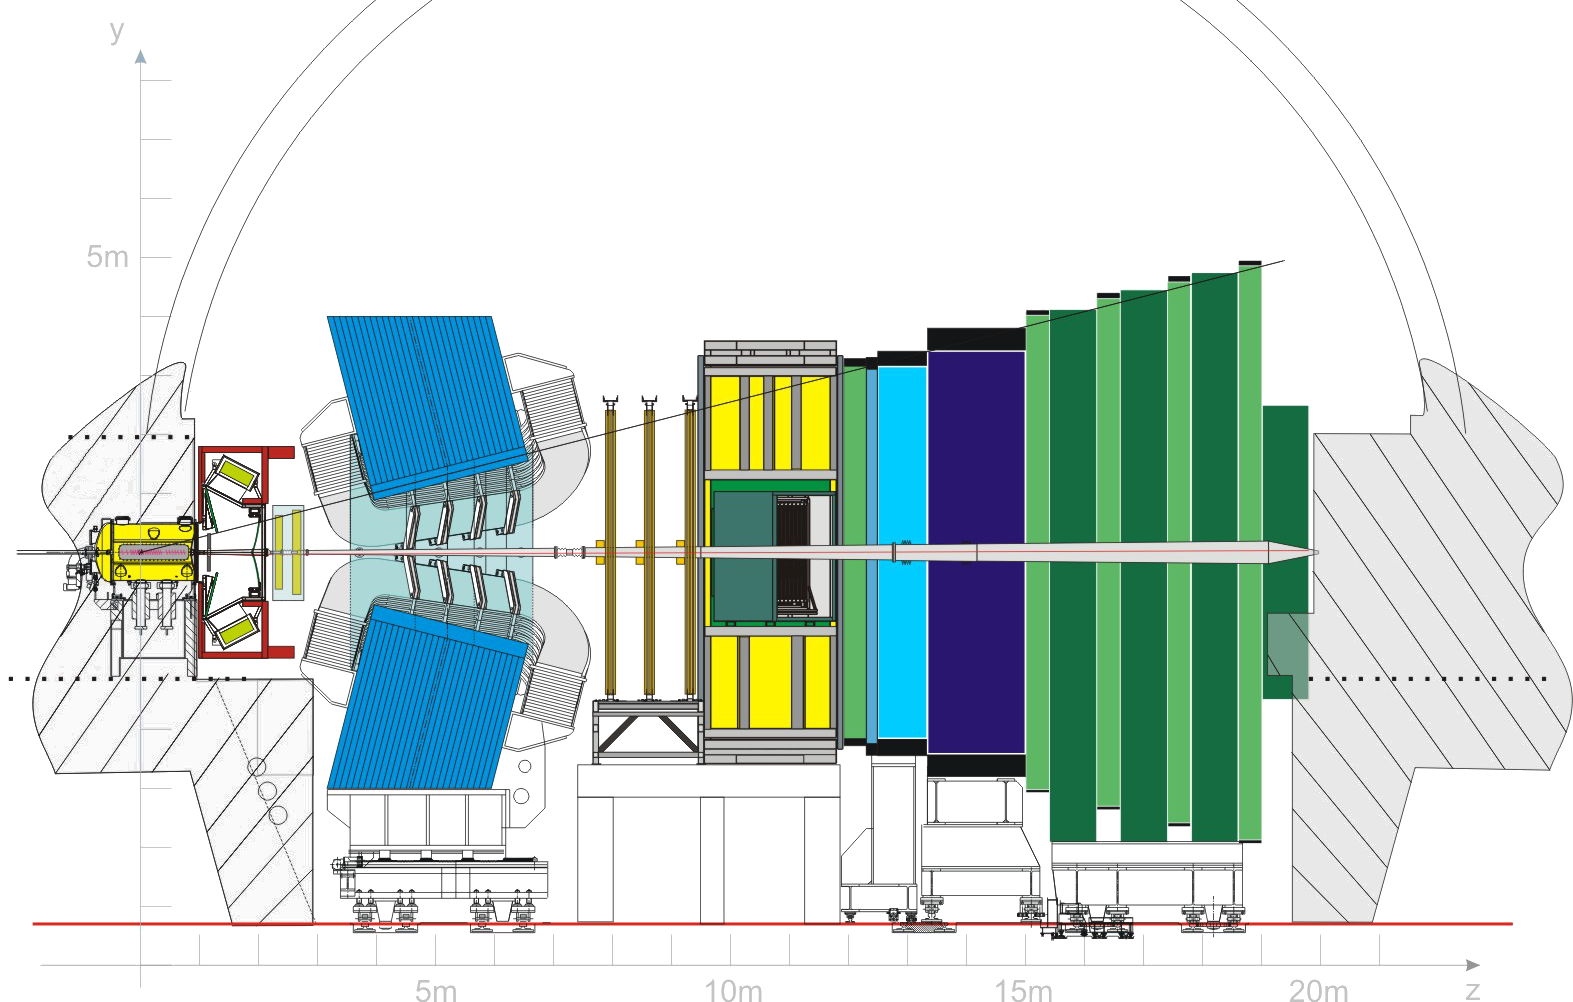
\includegraphics[width=1.\textwidth]{detector/LHCb}};
        \begin{scope}[x={(image.south east)},y={(image.north west)}]
            \draw [very thick, ->] (-.1, .45) -- (.01, .45) node [at start,anchor=north west] {\normalsize \proton};
            \draw [very thick, ->] (.95, .45) -- (.84, .45) node [at start,anchor=north east] {\normalsize \proton};

            \draw [very thick] (.11, .47) -- (.11, 0.85) node [right,anchor=north west,inner ysep=0pt,outer sep=0pt] {\velo};
            \draw [very thick] (.16, .54) -- (.16, 0.80) node [right,anchor=north west,inner ysep=0pt,outer sep=0pt] {\rich~1};
            \draw [very thick] (.185,.48) -- (.185,0.75) node [right,anchor=north west,inner ysep=0pt,outer sep=0pt] {\ttracker};
            \draw [very thick] (.27, .65) -- (.27, 0.85) node [right,anchor=north west,inner ysep=0pt,outer sep=0pt] {Magnet};
            \draw [very thick] (.413,.57) -- (.413,0.85) node [right,anchor=north west,inner ysep=0pt,outer sep=0pt] {\intr~\&~\ot};
            \draw [very thick] (.46, .61) -- (.46, 0.78) node [right,anchor=north west,inner ysep=0pt,outer sep=0pt] {\rich~2};
            \draw [very thick] (.57, .61) -- (.57, 0.85) node [right,anchor=north west,inner ysep=0pt,outer sep=0pt] {\presh~\&~\ecal};
            \draw [very thick] (.62, .63) -- (.62, 0.78) node [right,anchor=north west,inner ysep=0pt,outer sep=0pt] {\hcal};
            \draw [very thick] (.75, .67) -- (.75, 0.85) node [right,anchor=north west,inner ysep=0pt,outer sep=0pt,align=left] {Muon\\stations};
        \end{scope}
    \end{tikzpicture}
    \caption{
        Cutout of the \lhcb~detector, with the magnet and the various subdetectors indicated.
        The \({\proton\proton}\)~collisions occur on the left side of the figure, inside the~\velo.}
    \label{fig:detector_LHCb}
\end{figure}

\subsection{Tracking and vertexing}
\label{sec:tracking}

Tracking in the \lhcb~detector is performed by four subdetectors: the Vertex~Locator (\velo) and the double-layered~\ttracker upstream of the magnet, three stations of Inner and Outer Trackers (\intr and \ot), and five Muon stations downstream of the magnet.

The \velo~\cite{LHCb-DP-2014-001} consists of \num{42}~modules of silicon strip detectors centred around the beam pipe, with strips oriented in the radial and angular directions.
The silicon is cooled to an operational temperature of~\SI{-7}{\degreeCelsius}, and a motion system can move the modules closer to the beam pipe after the proton beams in the~\lhc have been focused, until the modules arrive at a distance of~\SI{8}{\mm} from the beam pipe.
The modules are semi-circular, and are placed in pairs of R-sensors (radial strips) and \(\phi\)-sensors (circular strips), which together allow for three-dimensional track reconstruction.
This setup gives a vertex resolution of~\SI{71}{\micro\meter} along the beam axis and \SI{13}{\micro\meter}~in the transverse plane.

The \ttracker~\cite{Gassner:728548} and \intr~\cite{LHCb-TDR-008} also both employ silicon strips to detect particles.
The~\ttracker is located upstream of the magnet, and consists of two stations.
The \intr~has three stations, and is located downstream of the magnet, close to the \lhc~beam pipe.
Each station contains four detection layers, of which the outer two are oriented vertically, and the inner two at a \(\pm\ang{5}\)~stereo angle.
These trackers each have a hit resolution of about~\SI{50}{\micro\meter}.
The \ot~\cite{LHCb-DP-2013-003} surrounds the \intr, and is made up of three stations of gas detectors.
Again, each station consists of four planes of straw tube modules, oriented the same way as in the~\ttracker and~\intr.
The \ot has a hit resolution of about~\SI{200}{\micro\meter}.
Finally, the muon system~\cite{LHCb-DP-2012-002,LHCb-DP-2013-001} consists of five stations of multi-wire proportional chambers (MWPCs), four of which are located downstream from the calorimeter systems, such that muons can be identified as they traverse the calorimeters, while keeping most of their momentum.
Due to the high particle density in the muon detector upstream of the calorimeter, its inner part is equipped with gas electron multiplier (\gem)~chambers.

Together, the tracking stations allow for the finding and fitting of tracks, the latter of which is done using a Kalman filter approach~\cite{Hulsbergen2005566}.
However, sometimes tracks are reconstructed from hits that do not correspond to the same physical object.
Such a nonphysical track is called a ghost track.
Neural networks are trained to identify them and yield an estimate of the probability of any particular track being a ghost track, allowing rejection of probable ghost tracks.
The most discriminating quantity in determining whether a track is a ghost track is the track~\chisqndf, which is defined as the~\chisq of the track fit divided by the number of degrees of freedom of that fit.
Low values indicate a good track fit, and correspondingly a low probability of that track being a ghost track.

\begin{figure}[htb] \centerfloat
    \begin{tikzpicture}[font=\captionfont]
        \coordinate (PV) at (0, 0);
        \coordinate (p1) at (-3, 0);
        \coordinate (p2) at (3, 0);
        \coordinate (Bs) at (2, 1);
        \coordinate (comp) at (6, 0.5);
        \coordinate (Ds) at (5, 2);
        \coordinate (h1) at (6, 2.25);
        \coordinate (h2) at (6, 2);
        \coordinate (h3) at (6, 1.75);

        \draw [thick,->] (p1) -- (PV) node [at start,anchor=north west] {\normalsize \proton} node [at end,anchor=north] {PV};
        \draw [thick,->] (p2) -- (PV) node [at start,anchor=north east] {\normalsize \proton};
        \draw [dashed] (PV) -- (Bs) node [midway,above,sloped] {\Bs} node [at end,anchor=south] {SV};
        \draw (Bs) -- (comp) node [midway,below,sloped] {companion};
        \draw [dashed] (Bs) -- (Ds) node [midway,above,sloped] {\Dspm};
        \draw (Ds) -- (h1) node [midway,below,sloped] {};
        \draw (Ds) -- (h2) node [midway,below,sloped] {};
        \draw (Ds) -- (h3) node [midway,below,sloped] {};
    \end{tikzpicture}
    \caption{
        Typical decay topology of decays under study in this thesis.
        The thick lines represent \lhc~protons, which collide at the primary vertex~(PV) inside the~\velo.
        In the collision, a \Bs~meson is formed, which flies through the detector undetected (dashed line) and subsequently decays at the secondary vertex (SV) into a \Dspm~meson and a charged hadron (solid line).
        This charged hadron is called the companion.
        The \Dspm~meson, in turn, travels some distance before decaying into three charged hadrons, called the \Dspm~daughters.
        In the end, four tracks are reconstructed in the detector, from which the topology is then deduced.}
    \label{fig:detector_topology}
\end{figure}

An unstable particle can be identified by the intersection of the tracks corresponding to its decay products.
\Cref{fig:detector_topology} shows the decay topology corresponding to the decays used in the analyses presented in this thesis.
To identify specific particle decays, as well as to suppress backgrounds, the invariant mass of a candidate is reconstructed from the momenta of these tracks.
In addition, the distance between two vertices, together with the momentum of the reconstructed particle, allows determination of its proper decay time.
The uncertainty of a decay-time determination is dominated by the vertex resolution, whereas both the uncertainty on the momentum and the vertex resolution contribute equally to the uncertainty on the mass.
An example distribution of flight distance of \bquark~mesons is shown in \cref{fig:detector_FD}.

\begin{figure}[htb] \centerfloat
    \begin{tikzpicture}
        \node[anchor=south west,inner sep=0] (image) at (0,0) {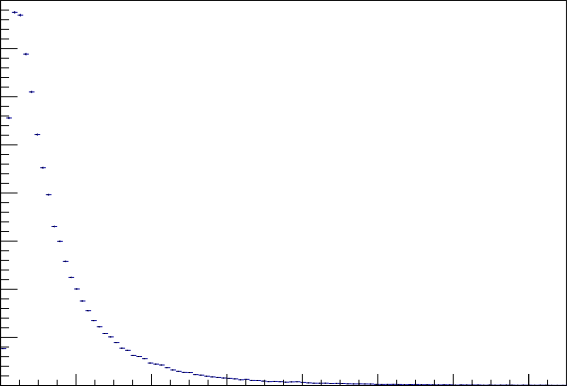
\includegraphics[width=0.8\textwidth]{detector/lab0_FD_OWNPV}};
        \begin{scope}[x={(image.south east)},y={(image.north west)}]
            \foreach \x in {0, ..., 7}
            {
                \tikzmath{\xpos = (\x / 7) * 0.934; \xtext = 20 * \x;}
                \node at (\xpos, -0.027) {\pgfmathprintnumber[fixed,precision=0,fixed zerofill=true]{\xtext}};
            }
            \foreach \y/\ytext in {0, ..., 8}
            {
                \tikzmath{\ypos = (\y / 8); \ytext = 10 * \y;}
                \node[anchor=east] at (0.005, \ypos) {\pgfmathprintnumber[fixed,precision=0,fixed zerofill=true]{\ytext}};
            }
            \node[anchor=south] at (0.03, 1.) {\({\times \num{e3}}\)};
            \node[anchor=east] at (1.0, -0.10) {\Bs~flight distance~[\si{\mm}]};
        \end{scope}
    \end{tikzpicture}
    \caption{
        Flight distance distribution of the \Bs~candidates from simulated \BsDsPi~decays.
        The exponential decrease corresponds with the decay of particles. The steep turn-on for small distances is caused by the acceptance of the \lhcb~trigger.}
    \label{fig:detector_FD}
\end{figure}

\subsection{Calorimetry}
\label{sec:calorimetry}

Downstream of the tracking detectors two calorimeters are located: an electromagnetic calorimeter~(\ecal) and a hadronic calorimeter (\hcal)~\cite{Perret:2015pla}.
The calorimeters are designed to stop most incoming particles and provide a measurement of their energy.
The \ecal detects electrons and photons, using an array of scintillating material of about \num{25}~radiation lengths to produce an electromagnetic shower response.
A single layer of scintillating pads~(\spd) is situated directly upstream of the~\ecal.
The pads track charged particles, and can therefore aid in distinguishing between electron and photon clusters in the~\ecal.
Finally, a two radiation lengths thick preshower detector~(\presh) is located directly upstream of the~\ecal, distinguishing electrons and photons from hadrons, as the latter are less likely to produce a contained shower.

The~\hcal has a thickness of \num{5.6}~radiation lengths.
It uses iron as absorber and scintillating tiles as active material.
It is designed to absorb all hadrons, allowing only muons to traverse into the downstream muon detectors.

\subsection{Particle identification}
\label{sec:det_pid}

Particle identification is obtained by a combination of the two Ring-Imaging~Cherenkov (\rich)~subdetectors, as well as the calorimeters and the muon stations.
The \rich{}es~\cite{LHCb-DP-2012-003} each consist of a container of active medium of different refractive index, which the produced particles traverse.
Whenever the speed of these particles exceeds the speed of light in one of these media, a cone-shaped burst of photonic Cherenkov radiation is emitted.
These photons are reflected in a set of mirrors mounted outside the fiducial volume of the container, and are subsequently picked up by arrays of photomultiplier tubes~(PMTs).
The diameter of a Cherenkov cone is a measure of the speed of the particle, which, together with its momentum as determined from the tracking detectors, allows determination of the particle's mass.
The \rich{}es are mostly used to discriminate between the various types of hadrons produced in the \({\proton\proton}\)~collisions: pions, kaons, and protons.
The active media used in~\rich1 and~\rich2 are~\cfourften, best suited for tracks with momenta up to~\SI{10}{\GeVc}, and~\cffour, for tracks with higher momenta up to~\SI{60}{\GeVc}, respectively.

To identify the other types of particles produced in the collisions, muons and electrons\footnote{The neutral particles that are also produced, \eg~photons, \piz~mesons, and neutrons, are not used by any of the analyses presented in this thesis, and therefore omitted from the discussion.}, the electromagnetic calorimeter and the muon stations are used.
Electrons are stopped by the electromagnetic calorimeter, and identified by their energy deposit.
Muons are the only particles traversing both the~\ecal and the~\hcal, and are identified by their tracks in the four muon stations located downstream of the calorimeters.

The data yielded by the~\rich{}es is analysed to yield quantitative information on the likelihood of a track belonging to a particle of a particular species.
The information of all RICH~PMTs from a single event is analysed simultaneously.
The algorithm starts by assuming the pion hypothesis for each track and computing the total likelihood under that assumption.
It then iteratively changes the hypothesis of each track if doing so improves the likelihood, until the maximum likelihood is reached.
The parameter of interest is then the difference in log-likelihood~(DLL) between two hypotheses.
For example, \dllkpi~represents the discrimination between the kaon and pion hypothesis of a track: a high value means the kaon hypothesis is more likely, while a low value tends towards the pion hypothesis.
\Cref{fig:detector_PID} demonstrates the necessity of using this information.

\begin{figure}[htb] \centerfloat
    \begin{tikzpicture}
        \node[anchor=south west,inner sep=0] (image) at (0,0) {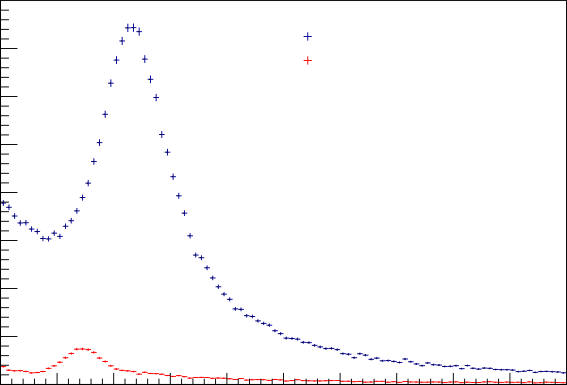
\includegraphics[width=0.8\textwidth]{detector/lab0_MM}};
        \begin{scope}[x={(image.south east)},y={(image.north west)}]
            \foreach \x in {0, ..., 10}
            {
                \tikzmath{\xpos = (\x / 10); \xtext = 50 * \x + 5300;}
                \node at (\xpos, -0.027) {\pgfmathprintnumber[fixed,precision=0,fixed zerofill=true,1000 sep={}]{\xtext}};
            }
            \foreach \y/\ytext in {1, ..., 8}
            {
                \tikzmath{\ypos = (\y / 8); \ytext = 1000 * \y;}
                \node[anchor=east] at (0.005, \ypos) {\pgfmathprintnumber[fixed,precision=0,fixed zerofill=true,1000 sep={}]{\ytext}};
            }
            % Legend
            {
                \node[anchor=base west] at (0.55, 0.890) {All data};
                \node[anchor=base west] at (0.55, 0.827) {With PID~selection};
            }
            \draw[gray,dashed] (.1338, 0.004) -- (.1338, 0.996) node [at end,below,rotate=90,anchor=south east,inner ysep=.5ex] {\tiny \Bs~mass};
            \node[anchor=east] at (1.0, -0.10) {\DsmpKpm~invariant mass~[\si{\MeVcc}]};
        \end{scope}
    \end{tikzpicture}
    \caption{
        The \DsmpKpm, \DsmpKKPi~invariant mass distribution of the full data set corresponding to an integrated luminosity of~\SI[mode=text]{3}{\per\femto\barn}, after the selection presented in \cref{sec:BsDsK_TD_Selection}, with and without PID selection on the companion track.
        The large peak in the distribution without the selection comes from misidentified \BsDsPi~decays, with a shifted mass due to the wrong mass hypothesis assigned to the companion track.
        The \BsDsK~mass peak (around~\SI{5367}{\MeVcc}) only becomes visible after a requirement on the \dllkpi~of the companion track.}
    \label{fig:detector_PID}
\end{figure}

\clearpage
\subsection{Trigger}
\label{sec:trigger}

The rate at which \({\proton\proton}\)~collisions take place in the detector is far greater than can conceivably be stored on disk.
In order to bring down the rate to a manageable level, a three-stage trigger~\cite{LHCb-DP-2012-004} selects only relevant events to be stored.
The first stage is a hardware trigger, called the Level~0 (\lzero)~trigger, which searches for tracks and clusters with high transverse momentum~(\pt) in the muon and calorimeter systems.
This stage brings the event rate down from \SI{40}{\MHz}~of collisions to an output rate of~\SI{1}{\MHz}.
The following two stages are both software-based, and these high-level triggers are called~\hltone and~\hlttwo.
They further reduce the event rate to a few~\si{\kHz}, which is low enough to allow storage on disk.
For the analyses presented in this thesis, the high-level triggers use a multivariate algorithm~\cite{Gligorov:2012qt} to require a vertex, displaced from the \({\proton\proton}\)~interaction point, consistent with the signature of a \bquark-meson decay (as illustrated in \cref{fig:detector_topology}).

\begin{figure}[htb] \centerfloat
    \begin{tikzpicture}
        \node[anchor=south west,inner sep=0] (image) at (0,0) {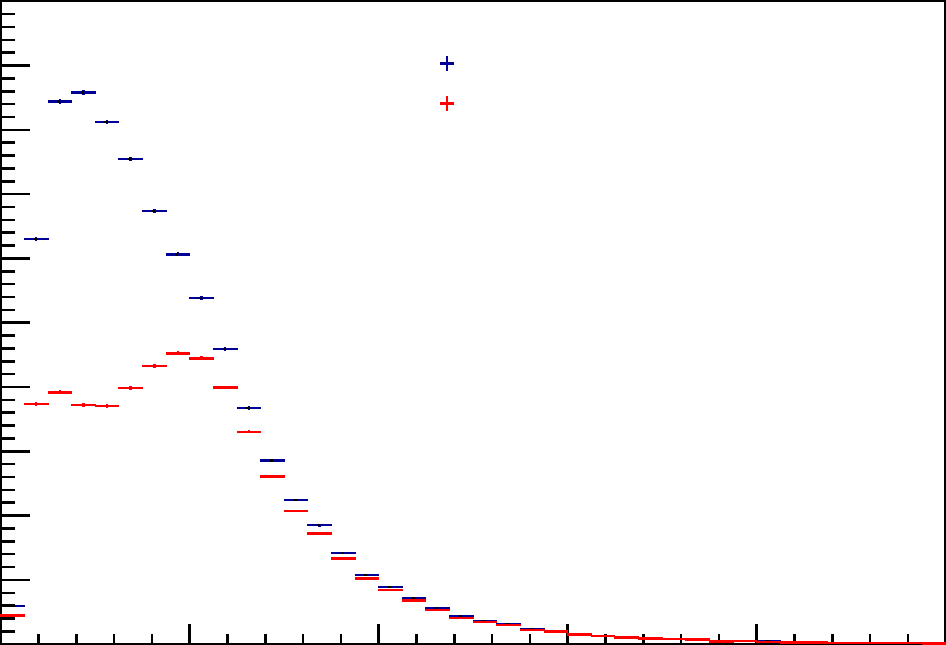
\includegraphics[width=0.8\textwidth]{detector/lab1_PT}};
        \begin{scope}[x={(image.south east)},y={(image.north west)}]
            \foreach \x in {0, ..., 5}
            {
                \tikzmath{\xpos = (\x / 5); \xtext = 5 * \x;}
                \node at (\xpos, -0.027) {\pgfmathprintnumber[fixed,precision=0,fixed zerofill=true,1000 sep={}]{\xtext}};
            }
            \foreach \y/\ytext in {0, ..., 10}
            {
                \tikzmath{\ypos = (\y / 10); \ytext = 10 * \y;}
                \node[anchor=east] at (0.005, \ypos) {\pgfmathprintnumber[fixed,precision=0,fixed zerofill=true,1000 sep={}]{\ytext}};
            }
            \node[anchor=south] at (0.03, 1.) {\({\times \num{e3}}\)};
            % Legend
            {
                \node[anchor=base west] at (0.480, 0.890) {All data};
                \node[anchor=base west] at (0.480, 0.827) {\lzero~triggered by companion};
            }
            \node[anchor=east] at (1.0, -0.10) {Companion~\pt~[\si{\GeVc}]};
        \end{scope}
    \end{tikzpicture}
    \caption{
        Transverse momentum distribution of companion \pipm~candidates from simulated \BsDsPi~decays, with and without the requirement that \lzero~triggered on the calorimeter cluster induced by that pion.
        It can be seen that for high-transverse momentum tracks, the \lzero~trigger usually triggered on those tracks, while for low-\pt~tracks it usually fired on another object in the event.}
    \label{fig:detector_companion_PT}
\end{figure}

\clearpage
\section{Simulation}
\label{sec:simulation}

In the analyses presented in this thesis, simulated samples are used to determine the selection efficiency of certain decays, as well as parameterise mass distributions of both signal and background channels.

The \proton\proton~collisions are generated using \pythia~\cite{Sjostrand:2007gs,Sjostrand:2006za} with a specific \lhcb configuration~\cite{LHCb-PROC-2010-056}.
Decays of hadronic particles are described by \evtgen~\cite{Lange:2001uf}, in which final-state radiation is generated using \photos~\cite{Golonka:2005pn}.
The interaction of the generated particles with the detector, and its response, are implemented using the \geant toolkit~\cite{Allison:2006ve,Agostinelli:2002hh} as described in Ref.~\cite{LHCb-PROC-2011-006}.
A software emulation of the \lzero~trigger is run on this response.
The next steps are the same as for data: \hltone, \hlttwo, and the reconstruction are applied, such that the simulated samples match the data as closely as possible.


    \clearpage
}

\ifthenelse{\boolean{ch-methods}}{
    \setchapterpreamble{
    \lettrine{T}{wo}~analyses are presented in this thesis: the first is an analysis of the branching fractions of~\BsDsK and~\BdDsK (\cref{chp:DsK_BF}), while the second is a measurement of the \CP-violation parameter~\CPgamma using the decay time of \BsDsK~events (\cref{chp:BsDsK_TD_Data,chp:BsDsK_TD}).
    Several experimental methods are common to these analyses: a loose event preselection (\cref{sec:stripping}), the use of multivariate methods to discriminate signal and background (\cref{sec:MVA}), the calibration of particle identification selection (\cref{sec:PID}), and the use of mass fits (\cref{sec:MassFits}).
    Although these tools are shared, the final selection of \BsDsK~events is re-optimised for the decay-time-dependent analysis, as described in \cref{chp:BsDsK_TD_Data}.}
\chapter{Experimental methods}
\label{chp:methods}

\vspace*{\fill}
\minitoc

\clearpage
\section{Event selection}
\label{sec:stripping}

A sophisticated selection of signal candidates is warranted, to reject as much background as possible while retaining most of the signal.
In general, each analysis features its own optimised selection, but a common preselection is used for decays of the form~\decay{\BorBsz}{\DorDsmp\hpm}, where \hpm~is one of~\pipm, \Kpm, or~\porpbar.
This~\lcnamecref{sec:stripping} outlines this preselection\footnote{
    In \lhcb~jargon, this preselection is known as the ``Stripping'' selection.}
, which is used by each of the analyses in the following chapters.

Firstly, there are several requirements on how events were processed by the triggers.
There are no requirements on the \lzero~response, and it is observed that for about~\SI{65}{\percent} of events one of the signal candidate tracks actually triggered the \lzero~trigger.
For~\hltone, events are required to have triggered using the \texttt{1TrackAllL0}~trigger line~\cite{Gligorov:1300771}, which requires the presence of a track with high momentum and low track~\chisqndf.
Such a track is likely to be a real signal track from a \bquark-hadron decay.
In~\hlttwo, events are selected that triggered on two- or three-body topological trigger~lines~\cite{hlt2toponote}.
These trigger~lines rely on the event topology (see \cref{fig:detector_topology}) and require a high-\pt two- or three-track secondary vertex that is significantly displaced from the primary vertex~(PV) and is consistent with the decay of a \bquark~hadron.
Additionally, events are selected that contain a \phiz~candidate, by requiring a two-track vertex consistent with a \PhiKK~decay~\cite{Gligorov:1362426}.
This selects decays in which a \bquark~hadron decays into a \Dsmp~meson, which subsequently decays into a \phiz~meson.

After the trigger, more selection is performed offline in order to obtain a pure signal sample, optimised to select events that contain a \bquark~hadron decaying into a \DorDsmp~meson and an accompanying hadron of opposite charge (the ``companion''~candidate).
These selection criteria are listed in \cref{tab:methods_stripping_cuts}.
Each candidate event is required to contain a combination of three particles consistent with the decay of a \DorDsmp~meson to one of the final states~\KmpKPi, \KmpPiPi, or~\PimpPiPi.
Each of these three \DorDsmp~daughter tracks must have a good track fit quality, high (transverse) momentum, and high impact parameter (IP)~\chisq,~\chisqip, with respect to any~PV, to signal its secondary nature.
The~\chisqip is defined as the difference in vertex fit~\chisq,~\chisqvtx, when fitting the vertex with and without the track under consideration, and a high value indicates that the track did not originate directly from that vertex.

If these requirements on individual tracks are passed, the three tracks are combined into a \DorDsmp~candidate.
This candidate is required to again have a large transverse momentum, an invariant mass in the region of the known masses of the \Dmp~and \Dsmp~mesons~\cite{PDG}, and a good \Dsmp~vertex fit.
Further requirements are a maximum distance of closest approach~(DOCA) between any two combinations of the three tracks and a large difference in~\chisqvtx of the best~PV when combining this vertex with that~PV, to ensure that the two are two separate, physical vertices.

To form a \bquark-hadron candidate, the \DorDsmp~candidate is combined with a companion track, which is again required to have good track fit quality, high (transverse)~momentum, and high~\chisqip with respect to any~PV.
Finally, the \bquark~hadron candidate combination must form a good vertex with the \DorDsmp~candidate and be significantly displaced from the best matching~PV.
It should also point back at this~PV, with a requirement on its~\chisqip with respect to that vertex, as well as on the cosine of the angle between its reconstructed momentum vector and the path to that~PV.
Furthermore, its invariant mass is required to fall within a wide mass window, covering the known masses of the \Bd~and \Bs~hadrons.
%
\begin{table}[htbp] \centerfloat
    \caption{
        Preselection requirements on the \bquark-hadron candidates and the tracks from which it is reconstructed.
        The invariant mass of the \DorDsmp~candidate is calculated under the hypotheses of its daughter tracks being each of~\KmpKPi, \KmpPiPi, or~\PimpPiPi, and the event is selected if at least one of these masses falls within the required window.
        Similarly, the \bquark-hadron candidate mass is calculated under both the pion and the kaon hypothesis for the companion candidate.}
    \label{tab:methods_stripping_cuts}
    \rowcolors{3}{}{tableshade}
    \begin{tabular}{ll}
        \toprule
        Variable & Requirement\tabularnewline
        \midrule
        \multicolumn{2}{l}{Each \DorDsmp~candidate daughter track} \tabularnewline
        \midrule

        Track~\chisqndf & \(< \num{3}\) \tabularnewline
        Ghost probability & \(< \num{0.4}\) \tabularnewline
        Transverse momentum & \(> \SI{100}{\MeVc}\) \tabularnewline
        Total momentum & \(> \SI{1}{\GeVc}\) \tabularnewline
        \chisqip~w.r.t. any~PV & \(> \num{4}\) \setcounter{rownum}{1}\tabularnewline[1ex]

        \midrule
        \multicolumn{2}{l}{At least one \DorDsmp~candidate daughter track} \tabularnewline
        \midrule

        Track~\chisqndf & \(< \num{2.5}\) \tabularnewline
        Transverse momentum & \(> \SI{500}{\MeVc}\) \tabularnewline
        Total momentum & \(> \SI{5}{\GeVc}\) \setcounter{rownum}{1}\tabularnewline[1ex]

        \midrule
        \multicolumn{2}{l}{\DorDsmp~candidate} \tabularnewline
        \midrule

        Invariant mass & \(\in \SI[parse-numbers=false]{[1770, 2068]}{\MeVcc}\) \tabularnewline
        \chisqvtxndf & \(< \num{10}\) \tabularnewline
        Transverse momentum & \(> \SI{1.8}{\GeVc}\) \tabularnewline
        Max. DOCA between any two tracks & \(\SI{0.5}{\mm}\) \tabularnewline
        Difference in best PV~\chisqvtxndf & \(> \num{36}\) \setcounter{rownum}{1}\tabularnewline[1ex]

        \midrule
        \multicolumn{2}{l}{Companion track} \tabularnewline
        \midrule

        Track~\chisqndf & \(< \num{2.5}\) \tabularnewline
        Ghost probability & \(< \num{0.4}\) \tabularnewline
        Transverse momentum & \(> \SI{500}{\MeVc}\) \tabularnewline
        Total momentum & \(> \SI{5}{\GeVc}\) \tabularnewline
        \chisqip~w.r.t. any~PV & \(> \num{4}\) \setcounter{rownum}{1}\tabularnewline[1ex]

        \midrule
        \multicolumn{2}{l}{\bquark-hadron candidate} \tabularnewline
        \midrule

        Invariant mass & \(\in \SI[parse-numbers=false]{[4750, 7000]}{\MeVcc}\) \tabularnewline
        \chisqvtxndf & \(< \num{10}\) \tabularnewline
        Decay time from best~PV & \(> \SI{0.2}{\ps}\) \tabularnewline
        \chisqip~w.r.t. best~PV & \(< \num{25}\) \tabularnewline
        \(\cos(\text{angle~with~best~PV})\) & \(> \num{0.999}\) \tabularnewline

        \bottomrule
    \end{tabular}
\end{table}

\clearpage
\section{Multivariate analysis}
\label{sec:MVA}

The most powerful step to separate signal from background uses a multivariate technique called a boosted decision tree~(BDT)~\cite{BDT}.
This algorithm receives as input two data samples, one signal and one background, and produces a classification as output which, based on the input, yields quantitative information on the likeliness of an event to be signal.

A Decision Tree operates by forming a tree structure, where each node represents a decision of a cut on the most discriminating variable.
Each node also has two child nodes, which follow the same structure for the subsamples on either side of the cut.
It is built by analysing the difference in signal and background distributions for each variable.
For the variable where they differ the most, it determines the optimal cut to discriminate the two samples, forming the first node.
This is repeated twice, once for input events that pass the cut and once for those that do not.
After a number of iterations, these nodes form a tree structure.
In the case of a \emph{boosted}~decision tree, this entire procedure is repeated a number of times, in each iteration applying weights to the training data: data points that were classified correctly in the previous iteration receive low weights, while data points that were classified incorrectly receive higher weights.
This allows the tree to fine-tune around difficult areas of phase space.

There are several parameters in a BDT that can be tuned, such as the number of boosting iterations, the maximum depth of each tree, and what method is used to scan variables to determine the optimal cutting point at each node.
After the classification has been produced, the receiver operating characteristic~(ROC) curve shows the background rejection as a function of the signal efficiency.
\Cref{fig:methods_ROCCurve} shows an example ROC~curve.
In the optimal case, this curve reaches the point~\({(1, 1)}\), where all background is rejected while simultaneously retaining all signal events.
In practice, the closeness of the curve to that point is a metric of the performance of the classification algorithm.
%
\begin{figure}[htb] \centerfloat
    \begin{tikzpicture}
        \node[anchor=south west,inner sep=0] (image) at (0,0) {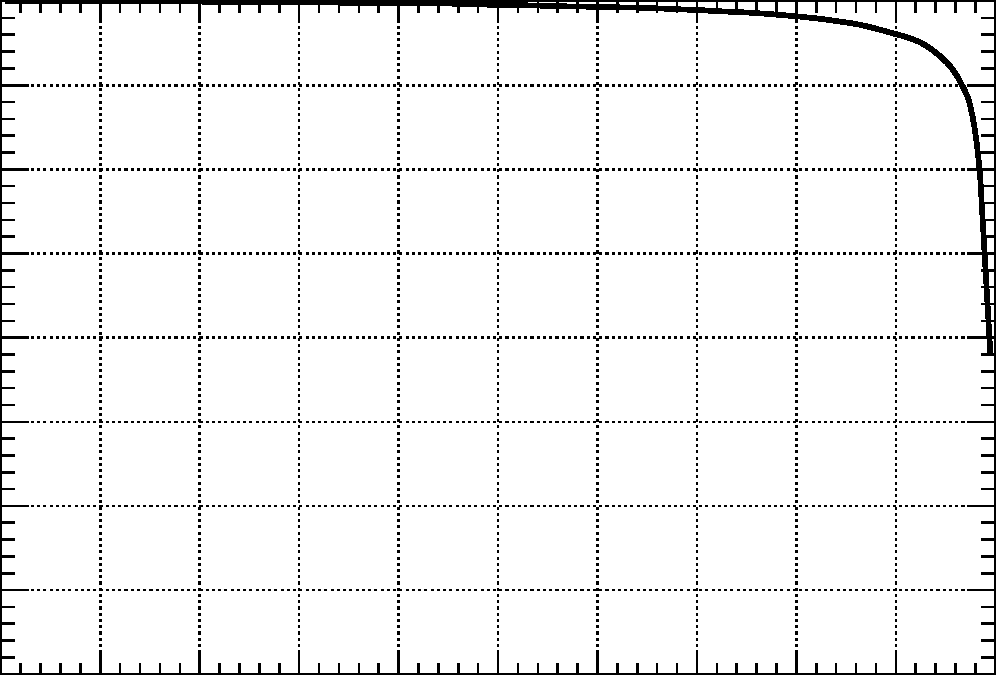
\includegraphics[width=0.9\textwidth]{BsDsK_TD/BDT/BDTG_RocCurve}};
        \begin{scope}[x={(image.south east)},y={(image.north west)}]
            \node at (0, -0.027) {\(0\)};
            \foreach \x in {1, ..., 10}
            {
                \tikzmath{\xtext = \x/10;}
                \node at (\x/10., -0.027) {\(\pgfmathprintnumber[fixed,precision=1,fixed zerofill=true]{\xtext}\)};
            }
            \foreach \y in {2, ..., 10}
            {
                \tikzmath{\ytext = \y/10; \ycoord = (\y - 1.97) / 8.07;}
                \node[anchor=east] at (0.005, \ycoord) {\(\pgfmathprintnumber[fixed,precision=1,fixed zerofill=true]{\ytext}\)};
            }
            \node[anchor=east] at (1.0, -0.10) {Signal efficiency};
            \node[rotate=90,anchor=east,inner xsep=0pt,outer xsep=0pt] at (-0.09, 1.0) {Background rejection};
        \end{scope}
    \end{tikzpicture}
    \caption{
        Example ROC~curve for the~BDT described in \cref{chp:BsDsK_TD_Data}, trained to separate \BsDsPi~events from combinatorial background.
        The black line parameterises a requirement on the classifier output, from very loose (top~left corner) to very tight (bottom~right corner).
        The optimal cutting point is somewhere in between, close to the top right corner.}
    \label{fig:methods_ROCCurve}
\end{figure}

\clearpage
\section{Particle identification}
\label{sec:PID}

The identification of particles~(PID) in~\lhcb is done by combining information from the~\rich, calorimeter and muon subdetectors.
However, since the efficiencies of correctly distinguishing pions, kaons, and protons are not well simulated, a data-driven method to determine the selection efficiency is warranted.

To determine the misidentification rate of pions and kaons, the decay \DstarDPi~is employed.
The pion originating directly from the \Dstarm~is labelled "S" to indicate that it is slow: due to the small mass difference between the \Dstarm~and \Dz~mesons there is only a small amount of phase space in the \Dstarm~decay, and so both the \Dz~and that pion are produced with low momenta in the \Dstarm~rest frame.
Identifying the slow pion by its momentum also allows identification of \Dz~decay products, using the charges of the respective tracks.
This allows unambiguous separation of pions and kaons using only tracking information, which can be used to calibrate the PID~efficiencies between pions and kaons from other subdetectors.

Similar to the procedure to calibrate the pion-kaon identification efficiency, the proton-pion efficiency can be calibrated, using the process \Lzppi.
Because of the mass difference between pions and protons, there is a momentum asymmetry between the decay products of \Lz~and \Lbar~baryons, which is exploited to distinguish the pion track from the proton track.

Each of these methods yields the efficiency of selecting a pion, kaon or proton for that specific decay.
However, different \bquark-hadron decays may have different properties.
In order to apply the efficiencies to such decays, they are computed as a function of track momentum, track transverse momentum, and number of tracks in the event.
An example of PID~efficiency as a function of kinematics can be seen in \cref{fig:Methods_PID_hist}.
Such a distribution can be used to calibrate the effect of a PID~requirement on a simulated sample, by reweighting the latter to the former.
Subsequently integrating also allows determining the total efficiency.
%
\begin{figure}[htb] \centerfloat
    \hspace*{-1cm}
    \begin{tikzpicture}
        \node[anchor=south west,inner sep=0] (image) at (0,0) {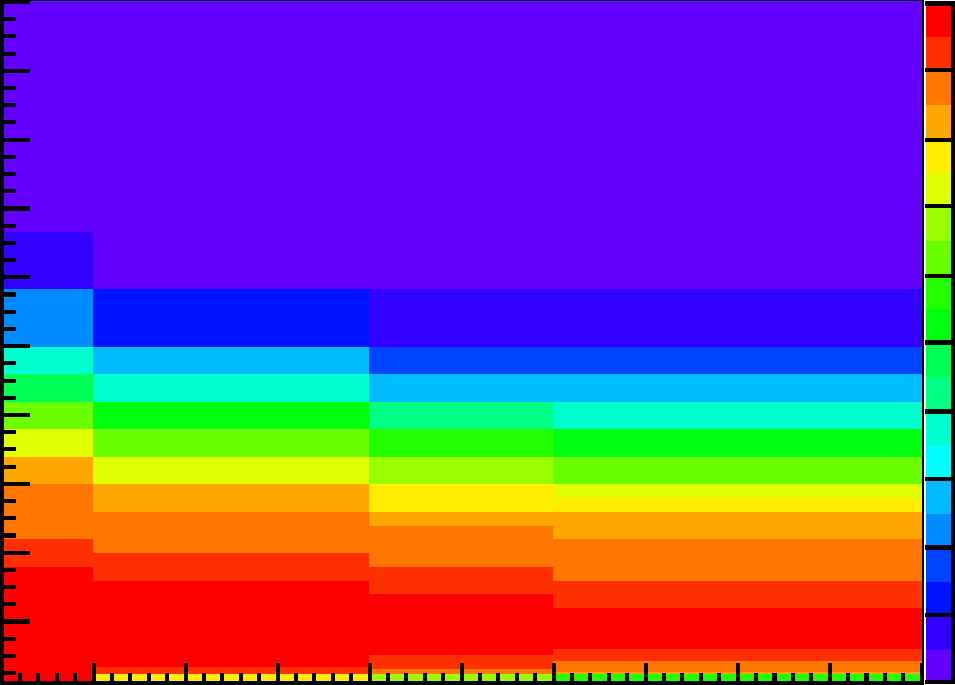
\includegraphics[width=0.9\textwidth]{methods/K_eff_PIDK5_2012_dw}};
        \begin{scope}[x={(image.south east)},y={(image.north west)}]
            \foreach \x/\xtext in {0, 50, ..., 500}
                \node at (\x/518, -0.025) {\(\xtext\)};
            \foreach \y/\ytext in {0, 20, ..., 200}
                \node[anchor=east] at (0.005, \y/201) {\(\ytext\)};
            \foreach \z in {0, ..., 10}
            {
                \tikzmath{\ztext = \z/10;}
                \node[anchor=west] at (1.0, 0.01 + \z/10.15) {\(\pgfmathprintnumber[fixed,precision=1,fixed zerofill=true]{\ztext}\)};
            }
            \node[anchor=east] at (1.0, -0.08) {Number of tracks in event};
            \node[rotate=90,anchor=east,inner xsep=0pt,outer xsep=0pt] at (-0.09, 1.0) {Track momentum [\si{\GeVc}]};
        \end{scope}
    \end{tikzpicture}
    \caption{
        Kaon selection efficiency for the requirement \({\dllkpi > 5}\), as a function of the number of tracks in the event (horizontal) and track momentum (vertical).
        These efficiencies are determined using decays of \Dstarm~mesons, following the data-driven method described in \cref{sec:PID}.
        The efficiency goes down as either the track momentum increases, which makes the distinction between pions and kaons by their speed harder; or as the track multiplicity increases, making Cherenkov ring reconstruction in the two~\rich{}es more difficult.}
    \label{fig:Methods_PID_hist}
\end{figure}

\clearpage
\section{Mass fits}
\label{sec:MassFits}

The yield of a specific signal decay is determined by performing a fit to the reconstructed invariant mass distribution of the final state.
Because mass is a unique property among hadrons, a peak in the mass distribution is attributed to decays of a particular parent hadron.
In order to perform a mass fit, several elements must be taken into account: signal, physics backgrounds, and combinatorial background.

\subsection{Signal}
\label{sec:MassFits_Signal}
The signal distribution takes the shape of a peak, centred around the mass of the parent hadron of interest.
Fundamentally, it takes the form of a Breit-Wigner shape, but the shape of relatively long-lived, weakly-decaying \bquark~hadrons in data is dominated by the resolution of the detector, which takes a Gaussian-like shape.
Additionally, radiation from the parent hadron causes a radiative tail to appear on the lower end of the mass spectrum.
The signal shape is parameterised using a double Crystal Ball~(DCB)~\cite{Skwarnicki:1986xj}, with a shared mean between the two Gaussian parts.
The central Gaussian functions describe the mass resolution, while the power-law tails account for the radiative tail on one side, and for events with poorly reconstructed mass on the other side.
The functional form of a DCB~shape is
%
\begin{multline} \label{eqn:Methods_DCB}
    \DCB(x; \DCBmu, \DCBsL, \DCBaL, \DCBnL, \DCBsR, \DCBaR, \DCBnR) = \\
    \begin{cases}
        \left(\dfrac{\DCBnL}{|\DCBaL|}\right)^{\DCBnL} e^{-\frac{1}{2}\DCBaL^2} \left[\dfrac{\DCBnL}{|\DCBaL|} - |\DCBaL| - \left(\dfrac{x - \DCBmu}{\DCBsL}\right)^{-\DCBnL}\right] &: \dfrac{x - \DCBmu}{\DCBsL} \leq \DCBaL \rlap{,} \\[3ex]
        e^{-\frac{1}{2} (x - \DCBmu)^2 / \DCBsL^2} &: \DCBaL\DCBsL < x - \DCBmu < 0 \rlap{,} \\[1ex]
        e^{-\frac{1}{2} (x - \DCBmu)^2 / \DCBsR^2} &: 0 > x - \DCBmu > \DCBaR\DCBsR \rlap{,} \\[1ex]
        \left(\dfrac{\DCBnR}{|\DCBaR|}\right)^{\DCBnR} e^{-\frac{1}{2}\DCBaR^2} \left[\dfrac{\DCBnR}{|\DCBaR|} - |\DCBaR| - \left(\dfrac{x - \DCBmu}{\DCBsR}\right)^{-\DCBnR}\right] &: \dfrac{x - \DCBmu}{\DCBsR} \geq \DCBaR \rlap{,}
    \end{cases}
\end{multline}
%
where \DCBmu~is the mean of the distribution, \DCBsLR~the widths of the central part left and right of~\DCBmu, \DCBaL~(\DCBaR) the distance to the left~(right) of~\DCBmu where the power-law tail starts, in units of \DCBsL~(\DCBsR), and \DCBnL~(\DCBnR) the slope of the left~(right) tail.
Often, the widths are taken to be equal, \({\DCBsL = \DCBsR = \DCBs}\), yielding a DCB with shared mean.
\Cref{fig:Methods_DCB_Examples} shows what such a distribution looks like. In general, a mass fit may have several signal components.
%
\begin{figure}[htb] \centerfloat
    \fontsize{9}{10.8}\selectfont
    \begin{subfigure}{.48\textwidth} \centerfloat
        \begin{tikzpicture}
            \node[anchor=south west,inner sep=0] (image) at (0,0) {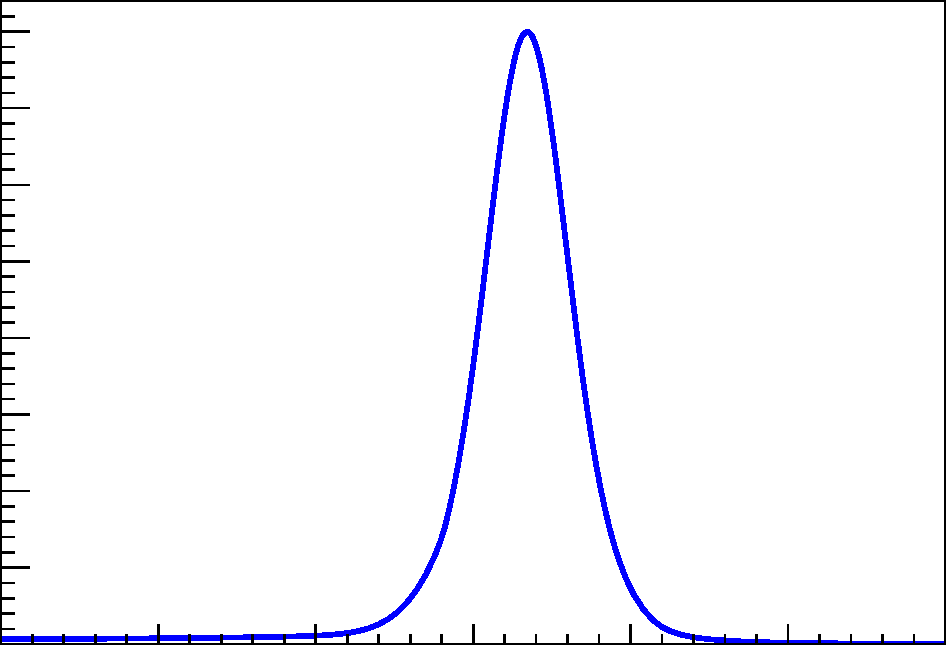
\includegraphics[width=0.9\textwidth]{methods/DCB_Example}};
            \begin{scope}[x={(image.south east)},y={(image.north west)}]
                \foreach \x in {0, ..., 6}
                {
                    \tikzmath{\xpos = (\x / 6); \xtext = 50 * \x + 5200;}
                    \node at (\xpos, -0.055) {\pgfmathprintnumber[fixed,precision=0,fixed zerofill=true,1000 sep={}]{\xtext}};
                }
                \node[anchor=east] at (1.0, -0.14) {\(x\)};
                \node[rotate=90,anchor=east,inner xsep=0pt,outer xsep=0pt] at (-0.07, 1.0) {\({\DCB(x)}\)};
            \end{scope}
        \end{tikzpicture}
    \end{subfigure} \hfill%
    \begin{subfigure}{.48\textwidth} \centerfloat
        \begin{tikzpicture}
            \node[anchor=south west,inner sep=0] (image) at (0,0) {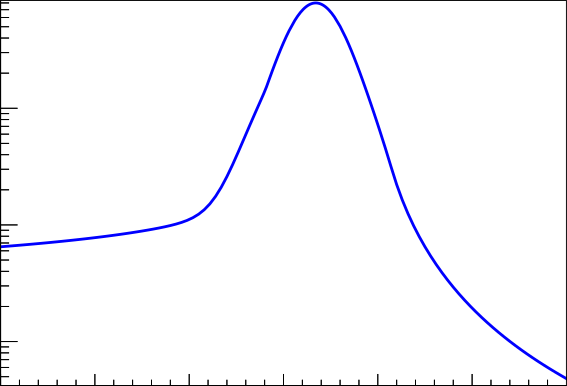
\includegraphics[width=0.9\textwidth]{methods/DCB_Example_log}};
            \begin{scope}[x={(image.south east)},y={(image.north west)}]
                \foreach \x in {0, ..., 6}
                {
                    \tikzmath{\xpos = (\x / 6); \xtext = 50 * \x + 5200;}
                    \node at (\xpos, -0.055) {\pgfmathprintnumber[fixed,precision=0,fixed zerofill=true,1000 sep={}]{\xtext}};
                }
                \node[anchor=east] at (1.0, -0.14) {\(x\)};
                \node[rotate=90,anchor=east,inner xsep=0pt,outer xsep=0pt] at (-0.07, 1.0) {\({\DCB(x)}\)};
            \end{scope}
        \end{tikzpicture}
    \end{subfigure}
    \caption{
        Example double Crystal Ball function, plotted in linear~(left) and logarithmic~(right) scale.
        The parameters are \({\DCBmu = \num{5367.11}}\), \({\DCBsL = \num{18.39}}\), \({\DCBsR = \num{11.43}}\), \({\DCBaL = \num{-2.19}}\), \({\DCBaR = \num{2.25}}\), \({\DCBnL = \num{2.37}}\), and \({\DCBnR = \num{0.42}}\), corresponding to the signal shape parameterisation used for \BsDsK, \DsmpPhiPi (see \cref{tab:BsDsK_TD_Signal_Shape_Results}) when \DCBmu~and \DCBsLR~are taken to be in units of~\si{\MeVcc}.
        Vertical units are omitted, as the normalisation is arbitrary.}
    \label{fig:Methods_DCB_Examples}
\end{figure}

\subsection{Physics backgrounds}
There are three distinguishable types of physics backgrounds: fully reconstructed backgrounds, partially reconstructed backgrounds, and misidentified backgrounds.
\begin{description}
\item[Fully reconstructed backgrounds] are decays with a different parent hadron but the same final state as the decay of interest.
    Their signal peak will be shifted with respect to that of the parent hadron, and therefore easily identifiable. These may very well be interesting in their own right, and may prompt further investigation.
\item[Partially reconstructed backgrounds] have the same final state as the parent hadron, apart from an extra decay product (such as a photon or a neutral pion), which is not accounted for in the reconstruction.
    The energy of the missing particle will also be absent in the invariant mass, which causes the distribution to be shifted to lower values, and smeared out. They have a shape which is difficult to model, and is generally extracted from simulation.
\item[Misidentified backgrounds] have a similar final state, but with a misidentified final-state particle.
    The shape of such a process is a smeared-out mass peak that is shifted with respect to that of the actual parent hadron.
\end{description}

Some backgrounds may belong to more than one category, such as partially reconstructed, misidentified backgrounds, or doubly partially reconstructed or doubly misidentified backgrounds.
These backgrounds have a small yield, so they do not have a large impact on a mass fit.

\subsection{Combinatorial background}
Combinatorial background results from random track combinations that happen to have an invariant mass close to that of the hadron of interest.
As such, these do not originate from any physical process, and the resulting distribution does not exhibit peaking structures.
It takes a negative exponential shape as a function of invariant mass, matching the number of random track combinations that can be made.
The exact parameters are difficult to determine from data, hence the usual strategy is to leave those parameters floating in the fit.

\subsection{Gaussian constraints}
If a parameter is known up to a certain uncertainty, such as the yield of a background process that can be calculated from prior information, it can be useful to constrain such a parameter in the mass fit.
One method to achieve that is to apply a Gaussian constraint to it.
This favours values for that parameter that are close to some predetermined mean value, as defined by a given width.
In a likelihood fit, such a constraint is taken into account by multiplying the likelihood by the deviation of the parameter value to that mean.
Multiple constraints can be taken into account, and the likelihood is multiplied with each.

\subsection{Kernel estimation} \label{sec:methods_KernelEstimation}
The shape of a distribution can often be taken directly from a representative simulated sample.
In order to use such a distribution in a mass fit, it must be transformed into a~PDF.
One way to achieve this is by using kernel estimation~\cite{Cranmer:2000du}.
This works by creating a Gaussian~function around each data point in the original distribution, adding those functions together, and normalising the resulting shape.
The width of the Gaussian~functions is a parameter that defines the smoothness of the resulting~PDF.


    \clearpage
}

\ifthenelse{\boolean{ch-dskbf}}{
    \chapter{The branching fractions of \BsDsK~and \BdDsK}
\label{chp:DsK_BF}

% Get the page number of Fig. 1 in the paper
\newcount\DsKBFFigPage
\DsKBFFigPage=\thepage
\advance\DsKBFFigPage by 3

\lettrine{T}{he}~branching fractions of the decays \BsDsK~and \BdDsK~are interesting for several reasons.
First of all, the process \BsDsK~is a benchmark for decay-time-dependent measurements of \CP~violation in tree decays, and a dedicated analysis of its branching fraction and its backgrounds aid such a measurement.
Furthermore, the branching fraction of the process~\BsDsK can be related to its counterpart~\BsDsPi using the known differences in CKM~factors, decay constants, and kinematic properties.
However, this ratio has been found to be in tension with the theoretical expectations~\cite{DeBruyn:2012jp}.
The decay~\BdDsK, in turn, is interesting since it occurs, to first order, only through the suppressed exchange topology (see Fig.~1 on Page~\the\DsKBFFigPage).
Therefore, a measurement of its branching fraction can yield information on exchange topologies in general.
The measurement of these branching fractions is published in \mbox{JHEP} under the title ``Determination of the branching fractions of \BsDsK and \mbox{\BdDsK''}~\cite{LHCb-PAPER-2014-064}\footnote{
    Author of this thesis is corresponding author of the publication, and main contributor to the analysis.}
, which is reproduced here as \cref{chp:DsK_BF} of this thesis.

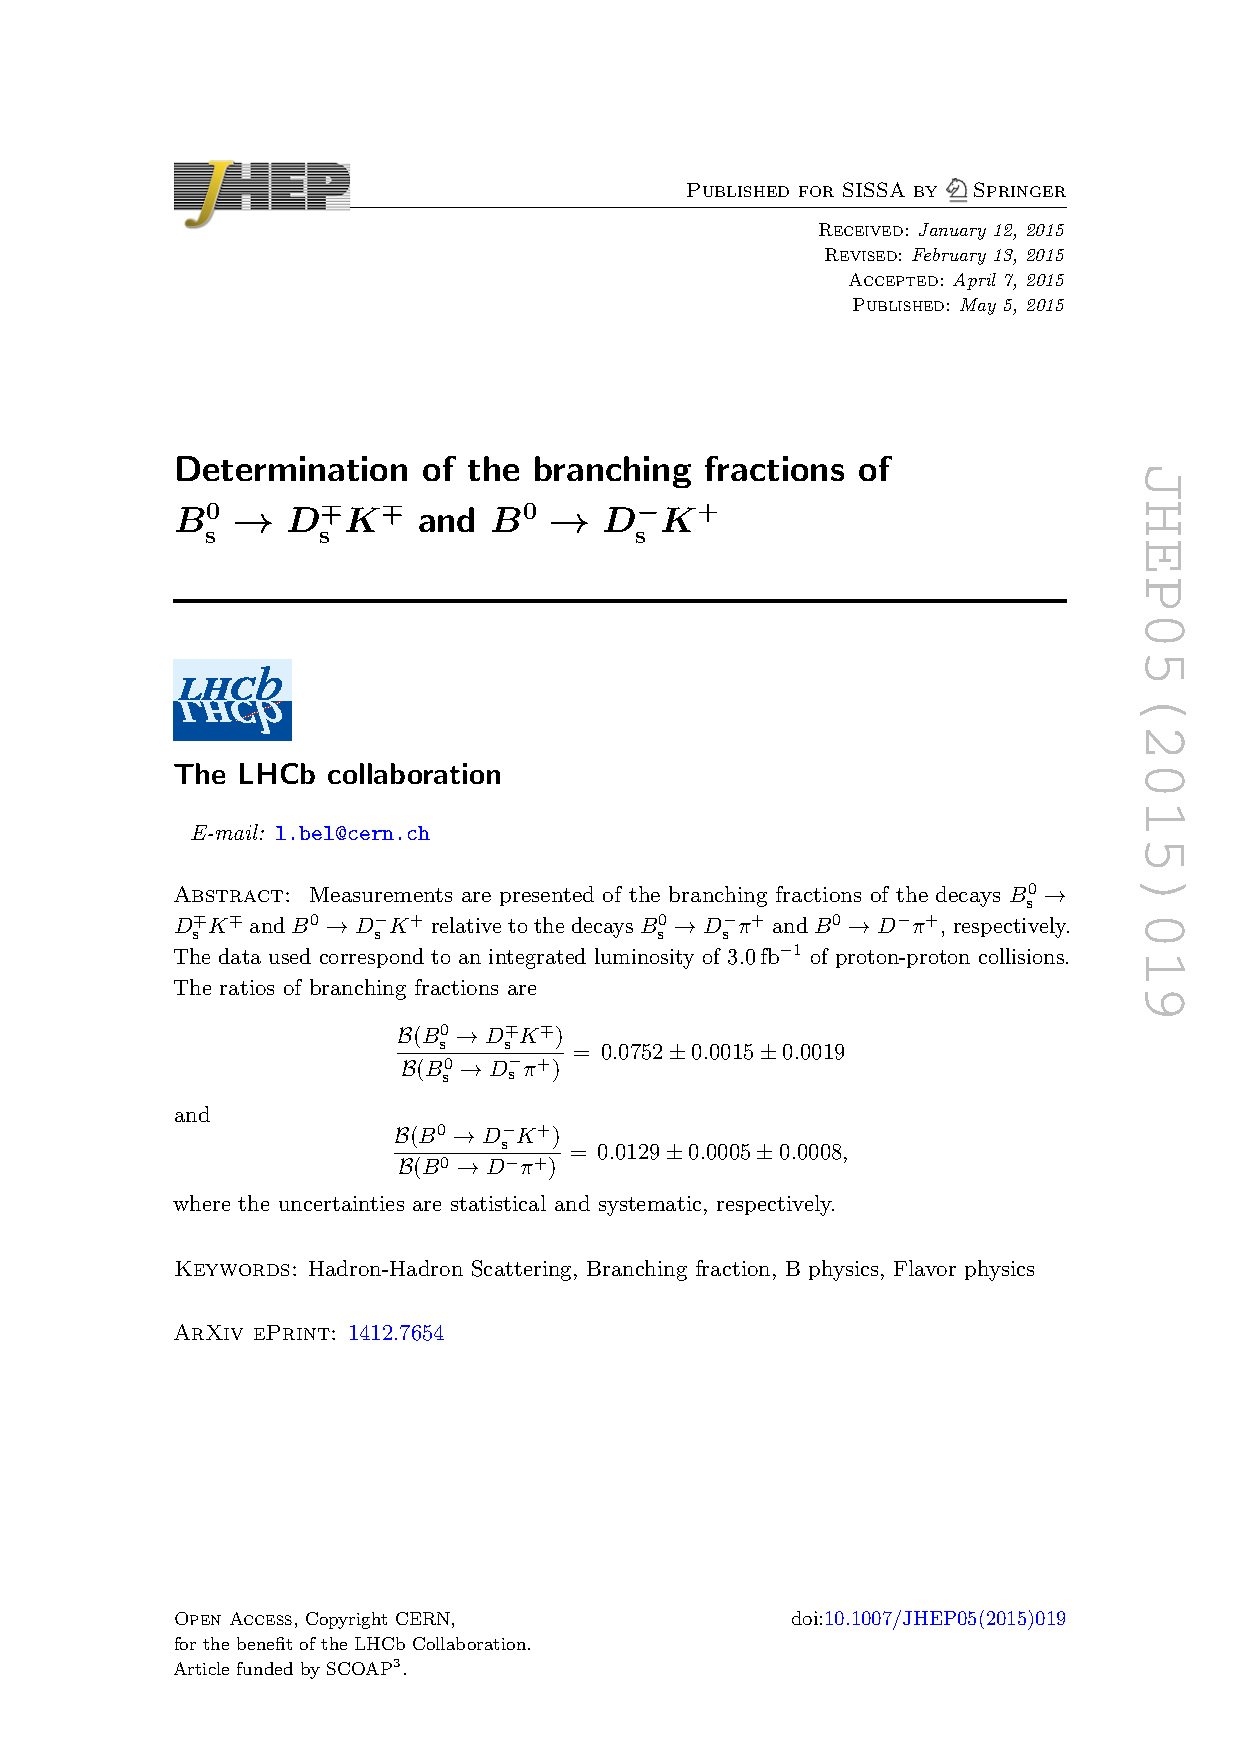
\includepdf[pages=-,scale=1.0,pagecommand={}]{includes/LHCb-PAPER-2014-064.pdf}


    \clearpage
}

\ifthenelse{\boolean{ch-bsdsktd}}{
    \addtocontents{toc}{\protect\newpage}
    \clearpage
\thispagestyle{plain}
\lettrine{F}{rom}~the decay-time spectrum of \BsDsK~events, the \CP-violation parameter~\CPgamma can be measured.
This is done in two steps: first, a statistically clean sample of \BsDsK~candidates is obtained, after which the decay-time distribution of this sample is fitted.
The complete analysis strategy is as follows.\\

\noindent \textbf{\large{\Cref{chp:BsDsK_TD_Data}}}
\vspace{.5ex}\hrule
\begin{enumerate}
    \item A clean sample of \BsDsK~signal candidates is selected, as well as kinematically similar \BsDsPi~candidates, which are used for calibration purposes.
    \item The \BsDsK~candidates are fitted, in order to subtract the background and obtain a statistically clean signal sample.
    \newcounter{enumvalue} \setcounter{enumvalue}{\value{enumi}}
\end{enumerate}

\noindent \textbf{\large{\Cref{chp:BsDsK_TD}}}
\vspace{.5ex}\hrule
\begin{enumerate}
    \setcounter{enumi}{\value{enumvalue}}
    \item Flavour tagging information on the resulting candidates is obtained and calibrated with the self-tagging \BsDsPi~candidates.
    \item The experimental decay-time measurement resolution is calibrated using a sample of prompt \Dsmp~events.
    \item \label{it:BsDsK_TD_Strat-dtfit} The \CP-violation parameters are extracted by fitting the decay time of the \Bs~sample, taking into account the tagging information, resolution, and acceptance corrections.
    \item The CKM~parameter \CPgamma~is determined from these parameters.
\end{enumerate}
%
The parameters extracted in step~\ref{it:BsDsK_TD_Strat-dtfit} are \({\Cpar = \Cbpar}\), \Spar, \Sbpar, \Dpar, and~\Dbpar, where~\({f = \DsmKp}\) (see \cref{sec:CPV}).

\clearpage

\setchapterpreamble{
    \lettrine{T}{his}~\lcnamecref{chp:BsDsK_TD_Data} discusses how a statistically pure sample of \BsDsK~candidates is obtained.
    In \cref{chp:DsK_BF}, a similar selection was discussed, which was aimed at obtaining the highest precision in yield and efficiency.
    Here, the selection is instead optimised to obtain for high signal purity, by suppressing as much background as possible.}
\chapter{\BsDsK~signal extraction}
\label{chp:BsDsK_TD_Data}

\vspace*{\fill}
\minitoc

\clearpage
\section{Data and selection}
\label{sec:BsDsK_TD_Selection}

\subsection{Data sample}
The data sample used for the analysis corresponds to an integrated luminosity of~\SI{3.0}{\per\femto\barn} of \({\proton\proton}\)-collision data recorded with the \lhcb~detector, of which \SI{1.0}{\per\femto\barn}~(\SI{2.0}{\per\femto\barn}) at \({\sqs = \SI{7}{\TeV}}\)~(\SI{8}{\TeV}).
About half of this data is taken with the opposite polarity of the \lhcb~magnet.
The preselection outlined in \cref{sec:stripping} is applied to this sample.
Candidates are reconstructed with the following final states\footnote{
    Charge conjugation is implied throughout this \lcnamecref{sec:BsDsK_TD_Selection}.}
(hereafter referred to as ``modes''):
%
\medskip
\begin{center}
\begin{tabular}{llp{5cm}}
    \toprule
    \BsDsK,  & \DsmKKPi   & The main signal channel;\tabularnewline[1ex]
    \BsDsK,  & \DsmPiPiPi & \multirow[t]{2}{=}{The \Dsm~branching fractions of these channels are lower, but they add to the statistics of the signal sample;} \tabularnewline
    \BsDsK,  & \DsmKPiPi  & \tabularnewline
    \tabularnewline
    \tabularnewline
    \midrule
    \BsDsPi, & \DsmKKPi   & \multirow[t]{3}{=}{This calibration channel is kinematically very similar to~\BsDsK, and has comparatively large statistics;} \tabularnewline
    \BsDsPi, & \DsmPiPiPi & \tabularnewline
    \BsDsPi, & \DsmKPiPi  & \tabularnewline
    \tabularnewline
    \midrule
    \BdDPi,  & \DmKPiPi   & This highly pure background channel is used to calibrate simulated data to better match the data.\tabularnewline
    \bottomrule
\end{tabular}
\end{center}
\medskip

\subsection{Boosted decision tree}

A~boosted decision tree\footnote{
    The BDT~configuration is defined as \num{300}~trees, each with a maximum depth of two nodes, while requiring that each node contains at least~\SI{4}{\percent} of the input events.
    The variables are scanned at \num{40}~points for the optimal cut value, and events with negative weights are excluded from the sample.}
(BDT, see \cref{sec:MVA}) is used to separate signal from combinatorial background events, which arises from random track combinations that look similar to signal candidates.
The signal input sample used to train this~BDT is chosen to be events of the plentiful decay~\BsDsPi with~\DsmKKPi, selected using the criteria listed in \cref{tab:BsDsK_TD_BDT_selection}.
Note that the companion track is defined as the pion not originating from the \Dsm~candidate (see \cref{sec:stripping}).
The tracks in the sample are refitted with the additional constraint that the \Bs~candidates originate from the closest~PV.
The signal is extracted from a fit to the \DsmPip~mass distribution which consists of a Gaussian shape for the signal and a negative exponential for the background, in which all parameters except the yields have been fixed to values obtained from simulation.
The background is statistically subtracted using the \sfit~method~\cite{Yuehong_sFit} to obtain a (statistically) pure signal sample.
The resulting mass distribution and fit are shown in \cref{fig:BsDsK_TD_BDT_Training_Data}.

As background input sample to train the~BDT, events from data in the upper mass region of the \DsmPip~invariant mass spectrum~(\({\SI[parse-numbers=false]{[5445, 5800]}{\MeVcc}}\)) are used.
Because there is no \Bs~signal in that region, this sample consists purely of combinatorial events, which are the events the~BDT is designed to reject.
Since no PID~information is used as input to the~BDT, the results are also valid for other \Dsm~decay channels with similar decay topology, such as~\DsmKPiPi and~\DsmPiPiPi.
%
\begin{table}[htb] \centerfloat
    \caption{
        \BsDsPi, \DsmKKPi~selection criteria for the sample used in the BDT~training.
        The same selection is applied to the charge-conjugated candidates.}
    \label{tab:BsDsK_TD_BDT_selection}
    \rowcolors{2}{tableshade}{}
    \begin{tabular}{lll}
        \toprule
        Description & Variable & Requirement\tabularnewline
        \midrule
        \DsmPip~mass & \(m(\DsmPip)\) & \(\in \SI[parse-numbers=false]{[5300, 5800]}{\MeVcc}\) \tabularnewline
        Companion~PID & \(\dllkpi(\pim)\) & \(< \num{0}\) \tabularnewline
        \Dsm~candidate mass & \(m(\Dsm)\) & \(\in \SI[parse-numbers=false]{[1940, 1990]}{\MeVcc}\) \tabularnewline
        \Dsm~daughters PID & \(\dllkpi(\Kmp)\) & \(> \num{0}\) \tabularnewline
        \Dm~veto & mass under \pim\Kp\pim hypothesis & \(< \SI{1850}{\MeVcc}\) \tabularnewline
        \hiderowcolors \aligncell{r}{\emph{or}} & \(\dllkpi(\Km)\) & \(> \num{10}\) \tabularnewline
        \showrowcolors\rowcolor{tableshade} \Lcm~veto & mass under \PbarKPi~hypothesis & \(\notin \SI[parse-numbers=false]{[2250, 2320]}{\MeVcc}\) \tabularnewline
        \aligncell{r}{\emph{or}} & \(\dllkp(\Km)\) & \(< \num{5}\) \tabularnewline
        \bottomrule
    \end{tabular}
\end{table}
%
\begin{figure}[tb] \centerfloat
    \hspace*{-1cm}
    \begin{tikzpicture}
        \node[anchor=south west,inner sep=0] (image) at (0,0) {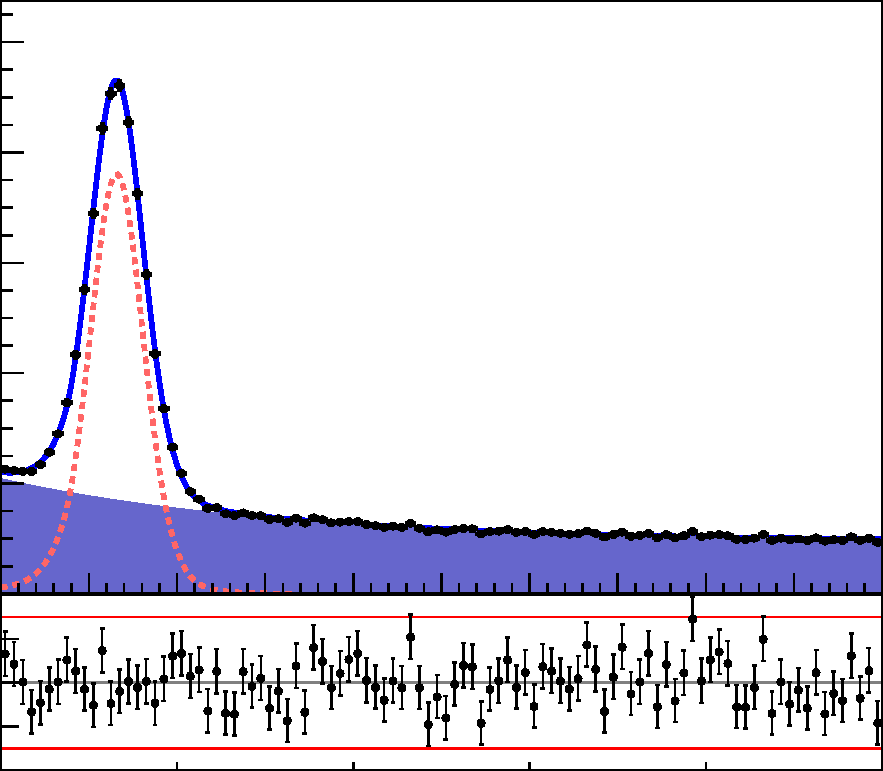
\includegraphics[width=0.9\textwidth]{BsDsK_TD/BDT/BDTG_Training_Bs2Dspi_FullSample_FullMassRange}};
        \begin{scope}[x={(image.south east)},y={(image.north west)}]
            \foreach \x/\xtext in {5300, 5400, ..., 5800}
            {
                \tikzmath{\xpos = (\x - 5300) / 500;}
                \node at (\xpos, -0.025) {\(\xtext\)};
            }
            \foreach \y/\ytext in {0, 2000, ..., 10750}
            {
                \tikzmath{\ypos = ((1 - 0.228) * \y) / 10750 + 0.228;}
                \node[anchor=east] at (0.005, \ypos) {\(\ytext\)};
            }
            \foreach \p/\ptext in {-2, 0, 2}
            {
                \tikzmath{\ypos = ((2 + \p) / 2 + 1) * (0.228 / 4);}
                \node[anchor=east] at (0.005, \ypos) {\(\scriptstyle\ptext\)};
            }
            \node[anchor=east] at (1.0, -0.08) {\({m(\DsmpPipm)}~[\si{\MeVcc}]\)};
            \node[rotate=90,anchor=east,inner xsep=0pt,outer xsep=0pt] at (-0.13, 1.0) {\({\text{Candidates}/(\SI{5}{\MeVcc})}\)};
            \node[anchor=east] at (0.95, 0.90) {\Huge\lhcb};
        \end{scope}
    \end{tikzpicture}
    \caption{
        \DsmpPipm~invariant mass distribution of the data sample used for the BDT~training, with a fit to the data superimposed.
        Note that a small amount of background events remain present in the signal sample, slightly reducing the BDT's~efficacy.}
    \label{fig:BsDsK_TD_BDT_Training_Data}
\end{figure}
%
\begin{figure}[tb] \centerfloat
    \scriptsize
    \begin{subfigure}{.45\textwidth} \centerfloat
        \begin{tikzpicture}
            \node[anchor=south west,inner sep=0] (image) at (0,0) {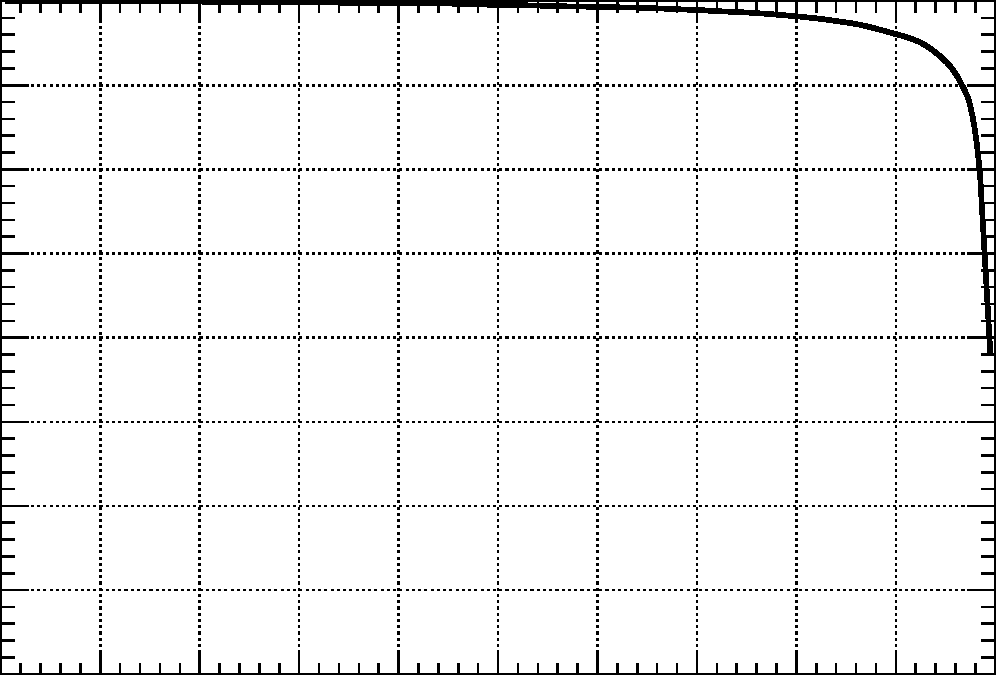
\includegraphics[width=0.9\textwidth]{BsDsK_TD/BDT/BDTG_RocCurve}};
            \begin{scope}[x={(image.south east)},y={(image.north west)}]
                \node at (0, -0.050) {\(0\)};
                \foreach \x in {1, ..., 10}
                    \tikzmath{\xtext = \x/10;}
                    \node at (\x/10., -0.050) {\(\pgfmathprintnumber[fixed,precision=1,fixed zerofill=true]{\xtext}\)};
                \foreach \y in {2, ..., 10}
                    \tikzmath{\ytext = \y/10; \ycoord = (\y - 1.97) / 8.07;}
                    \node[anchor=east] at (0.005, \ycoord) {\(\pgfmathprintnumber[fixed,precision=1,fixed zerofill=true]{\ytext}\)};
                \node[anchor=east] at (1.0, -0.15) {Signal efficiency};
                \node[rotate=90,anchor=east,inner xsep=0pt,outer xsep=0pt] at (-0.14, 1.0) {Background rejection};
            \end{scope}
        \end{tikzpicture}
    \end{subfigure} \qquad%
    \begin{subfigure}{.45\textwidth} \centerfloat
        \begin{tikzpicture}
            \node[anchor=south west,inner sep=0] (image) at (0,0) {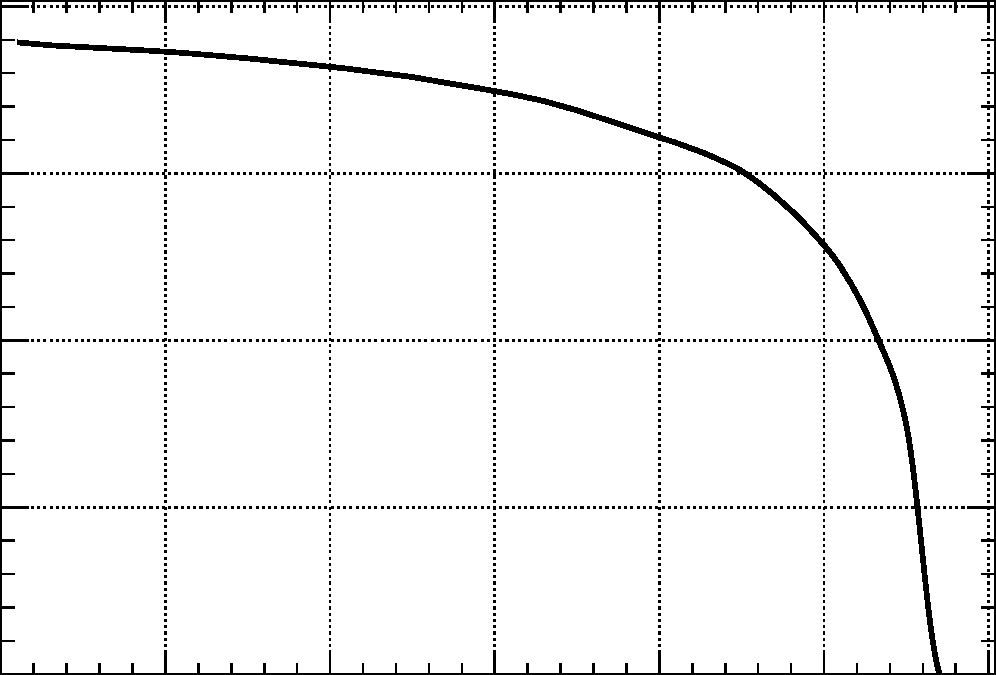
\includegraphics[width=0.9\textwidth]{BsDsK_TD/BDT/BDTG_RocCurve_Zoomed}};
            \begin{scope}[x={(image.south east)},y={(image.north west)}]
                \foreach \x in {7, 7.5, ..., 10}
                    \tikzmath{\xtext = \x/10; \xcoord = (\x - 7) / 3.;}
                    \node at (\xcoord, -0.050) {\(\pgfmathprintnumber[fixed,precision=2,fixed zerofill=true]{\xtext}\)};
                \foreach \y in {8, 8.5, ..., 10}
                    \tikzmath{\ytext = \y/10; \ycoord = (\y - 7.97) / 2.03;}
                    \node[anchor=east] at (0.005, \ycoord) {\(\pgfmathprintnumber[fixed,precision=2,fixed zerofill=true]{\ytext}\)};
                \node[anchor=east] at (1.0, -0.15) {Signal efficiency};
                \node[rotate=90,anchor=east,inner xsep=0pt,outer xsep=0pt] at (-0.18, 1.0) {Background rejection};
            \end{scope}
        \end{tikzpicture}
    \end{subfigure}
    \caption{
        Left: ROC curve for the trained~BDT.
        Right: the same plot, zoomed in on the interesting region near the top-right of the figure.}
    \label{fig:BsDsK_TD_BDT_Roc}
\end{figure}

To verify that overtraining did not occur, the samples are split randomly into two equally sized samples, and the~BDT is trained independently on each sample.
The receiver operator characteristic (ROC, see \cref{sec:MVA}) curve resulting from this training is shown in \cref{fig:BsDsK_TD_BDT_Roc}.
Afterwards, the~BDT is applied to each event in the sample it was not trained on, the results of which are shown in \cref{fig:BsDsK_TD_BDTResponse}.
From the figure it can be seen that the two~BDTs are compatible, and no overtraining occurred.
The BDT~output variable runs from~\num{-1} to~\num{1}, and for each selected event it is required to be~\({> \num{0.1}}\).
%
\begin{figure}[htb] \centerfloat
    \begin{tikzpicture}
        \node[anchor=south west,inner sep=0] (image) at (0,0) {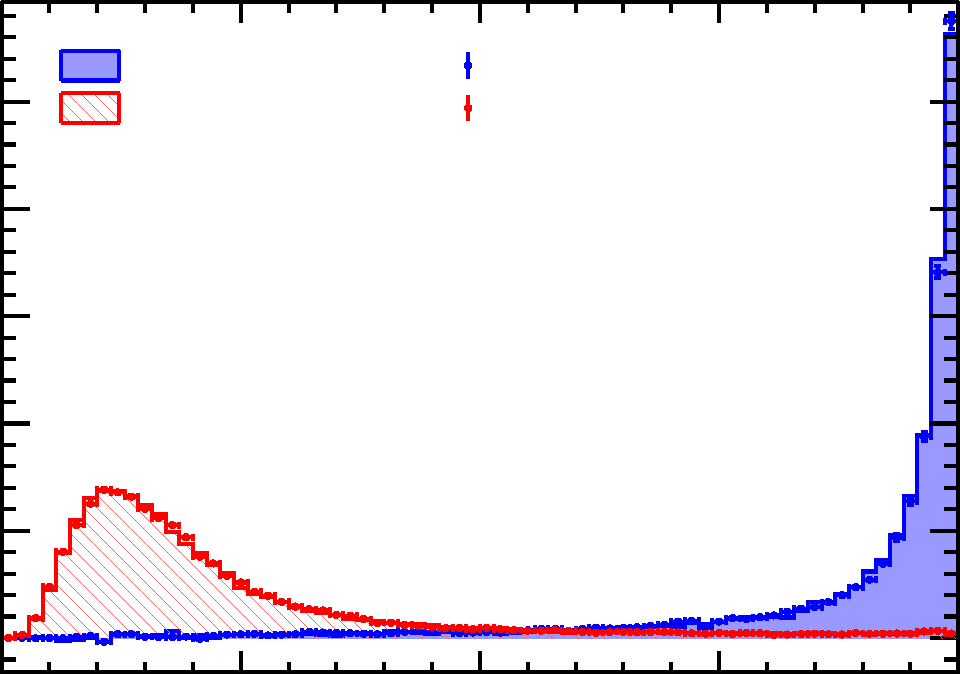
\includegraphics[width=0.9\textwidth]{BsDsK_TD/BDT/BDTG_Training_classifier_output}};
        \begin{scope}[x={(image.south east)},y={(image.north west)}]
            \foreach \x in {0, ..., 4}
                \tikzmath{\xtext = \x / 2 - 1; \xcoord = \x / 4;}
                \node at (\xcoord, -0.035) {\(\pgfmathprintnumber[fixed,precision=1,fixed zerofill=true]{\xtext}\)};
            \foreach \y in {0, ..., 5}
                \tikzmath{\ytext = \y / 20; \ycoord = \y / 6.28 + 0.055;}
                \node[anchor=east] at (0.005, \ycoord) {\(\pgfmathprintnumber[fixed,precision=2,fixed zerofill=true]{\ytext}\)};
            \node[anchor=east] at (1.0, -0.10) {BDT~response};
            \node[rotate=90,anchor=east,inner xsep=0pt,outer xsep=0pt] at (-0.09, 1.0) {Fraction of events};
            \node[anchor=west] at (0.13, 0.9) {Signal BDT~1};
            \node[anchor=west] at (0.13, 0.835) {Background BDT~1};
            \node[anchor=west] at (0.50, 0.9) {Signal BDT~2};
            \node[anchor=west] at (0.50, 0.835) {Background BDT~2};
        \end{scope}
    \end{tikzpicture}
    \caption{
        Output of the~BDTs when each is applied to the sample on which the other was trained.
        The two signal BDT~distributions (blue) match, as well as the two background distributions~(red), showing that neither~BDT was overtrained on specific features of its respective sample.}
    \label{fig:BsDsK_TD_BDTResponse}
\end{figure}

\subsection{\BsDsK~and \BsDsPi~signal candidates selection} \label{sec:BsDsK_TD_Selection_Signal}
Further selection of signal events is based on kinematic properties and identification of the candidates.
Selection criteria vary per \Dsm~decay mode, as summarised in \cref{tab:BsDsK_TD_Ds_Selection}.
For the \DsmKKPi~mode, the sample is split into three submodes, representing the decays \DsmPhiPi~(\PhiKK), \DsmKstK~(\KstKPi), and nonresonant \DsmKKPi~decays.
These have different PID~requirements: the resonances are relatively clean of background, justifying looser requirements on their daughter particles.
In contrast, the selection requirements on the nonresonant sample are stricter.
Each candidate only belongs to one of these categories; \ie if one is categorised as \DsmPhiPi~it is never classified as \DsmKstK, and if one is categorised as \DsmKstK it is not considered nonresonant, even if it would also satisfy the criteria for that submode.

Misidentified \DmKPiPi~(\LcmPKPi)~candidates are suppressed by vetoing any \Dsm~(\Lcm)~candidates whose mass in the \KpPimPim~(\PbarKPi)~mass hypothesis is close to the \Dm~(\Lcm)~mass, unless the~PID by itself is good enough (as specified in \cref{tab:BsDsK_TD_Ds_Selection}) to suppress misidentification.
Mode-independent selection criteria, as well as criteria on the \Bs~candidate (combination of \Dsm~candidate with a companion track), are listed in \cref{tab:BsDsK_TD_Selection}.
%
\begin{table}[htbp] \centerfloat
    \caption{
        Mode-dependent kinematic and PID~selection requirements for the \Dsm~candidates.
        The same selection is applied to the charge-conjugated candidates.}
    \label{tab:BsDsK_TD_Ds_Selection}
    \begin{tabular}{lll}
        \toprule
        Description & Variable & Requirement\tabularnewline
        \midrule
        \multicolumn{3}{l}{\DsmKKPi} \tabularnewline
        \midrule

        \Dsm~vertex separation & \chisq~w.r.t. \Bs~vertex & \(> \num{2}\) \tabularnewline
        \rowcolor{tableshade}\Dz~veto & \(m(\Km\Kp)\) & \(< \SI{1840}{\MeVcc}\) \tabularnewline

        \Dm~veto & mass under \({\pim\Kp\pim}\)~hypothesis & \(\notin \SI[parse-numbers=false]{[1840, 1900]}{\MeVcc}\) \tabularnewline
        \aligncell{r}{\emph{or}} & \(\dllkpi(\Km)\) & \(> \num{10}\) \tabularnewline

        \rowcolor{tableshade}\Lcm~veto & mass under \PbarKPi~hypothesis & \(\notin \SI[parse-numbers=false]{[2255, 2315]}{\MeVcc}\) \tabularnewline
        \rowcolor{tableshade}\aligncell{r}{\emph{or}} & \(\dllkp(\Km)\) & \(< \num{5}\) \tabularnewline
        \multicolumn{3}{l}{Submodes} \tabularnewline

        \quad\DsmPhiPi & \(m(\Km\Kp)\) & \(\in \SI[parse-numbers=false]{[1000, 1040]}{\MeVcc}\) \tabularnewline
        \aligncell{r}{\emph{and}} & \(\dllkpi(\Kmp)\) & \(> \num{-2}\) \tabularnewline

        \rowcolor{tableshade}\quad\DsmKstK & \(m(\Kp\pim)\) & \(\in \SI[parse-numbers=false]{[842, 942]}{\MeVcc}\) \tabularnewline
        \rowcolor{tableshade}\aligncell{r}{\emph{and}} & \(\dllkpi(\Kp)\) & \(> \num{-2}\) \tabularnewline
        \rowcolor{tableshade}\aligncell{r}{\emph{and}} & \(\dllkpi(\Km)\) & \(> \num{5}\) \tabularnewline

        \quad Nonresonant & \(\dllkpi(\Kmp)\) & \(> \num{5}\) \tabularnewline
        \aligncell{r}{\emph{and}} & \(\dllkpi(\pim)\) & \(< \num{10}\) \tabularnewline[1ex]

        \midrule
        \multicolumn{3}{l}{\DsmKPiPi} \tabularnewline
        \midrule

        \Dsm~vertex separation & \chisq~w.r.t. \Bs~vertex & \(> \num{9}\) \tabularnewline
        \rowcolor{tableshade}\Dz~veto & \(m(\Km\pip)\) & \(< \SI{1750}{\MeVcc}\) \tabularnewline

        \Dm~veto & mass under \({\pim\Kp\pim}\)~hypothesis & \(\notin \SI[parse-numbers=false]{[1840, 1900]}{\MeVcc}\) \tabularnewline
        \aligncell{r}{\emph{or}} & \(\dllkpi(\Km)\) & \(> \num{20}\) \tabularnewline
        \aligncell{r}{\emph{or}} & \(\dllkpi(\pip)\) & \(< \num{-10}\) \tabularnewline

        \rowcolor{tableshade}\Lc~veto & mass under \PbarKPi~hypothesis & \(\notin \SI[parse-numbers=false]{[2255, 2315]}{\MeVcc}\) \tabularnewline
        \rowcolor{tableshade}\aligncell{r}{\emph{or}} & \(\dllkp(\Km)\) & \(< \num{5}\) \tabularnewline

        PID~requirements & \(\dllkpi(\Km)\) & \(> \num{10}\) \tabularnewline
        \aligncell{r}{\emph{and}} & \(\dllkpi(\pipm)\) & \(< \num{5}\) \tabularnewline
        \aligncell{r}{\emph{and}} & \(\dllkp(\pipm)\) & \(< \num{10}\) \tabularnewline[1ex]

        \midrule
        \multicolumn{3}{l}{\DsmPiPiPi} \tabularnewline
        \midrule
        \Dsm~vertex separation & \chisq~w.r.t. \Bs~vertex & \(> \num{9}\) \tabularnewline
        \rowcolor{tableshade}\Dz~veto & \(m(\pim\pip)\)~(both combinations) & \(< \SI{1700}{\MeVcc}\) \tabularnewline

        PID~requirements & \(\dllkpi(\pimp)\)~(for each pion) & \(< \num{10}\) \tabularnewline
        \aligncell{r}{\emph{and}} & \(\dllkp(\pimp)\)~(for each pion) & \(< \num{10}\) \tabularnewline
        \bottomrule
    \end{tabular}
\end{table}
%
\begin{table}[htb] \centerfloat
    \caption{
        Mode-independent kinematic and PID~selection requirements for the \BsDsK~and \BsDsPi~candidates.
        The \Dsmp~candidates are reconstructed as specified in \cref{tab:BsDsK_TD_Ds_Selection}, and the companion track is the \Kpm~or \pipm~candidate that is combined with the \Dsmp~candidate form the \Bs~candidate.}
    \label{tab:BsDsK_TD_Selection}
    \begin{tabular}{lll}
        \toprule
        Description & Variable & Requirement\tabularnewline
        \midrule
        \Bs~decay time & decay time w.r.t.~PV & \(> \SI{0.4}{\ps}\) \tabularnewline
        \rowcolor{tableshade}\Bs~invariant mass & \({m(\Bs)}\) & \(\in \SI[parse-numbers=false]{[5300, 5800]}{\MeVcc}\) \tabularnewline
        Companion~PID & \({\dllkpi(\text{companion})}\) & \(< \num{0}\) for the \pion~hypothesis \tabularnewline
        & & \(> \num{5}\) for the \kaon~hypothesis \tabularnewline
        \rowcolor{tableshade}Semileptonic veto & \(\dllmupi(\text{companion})\) & \(< \num{2}\) \tabularnewline
        \midrule
        \Dsmp~decay time & decay time w.r.t. \Bs~vertex & \(> \num{0}\) \tabularnewline
        \rowcolor{tableshade}\Dsmp~invariant mass & \({m(\Dsmp)}\) & \(\in \SI[parse-numbers=false]{[1930, 2015]}{\MeVcc}\) \tabularnewline
        \bottomrule
    \end{tabular}
\end{table}

\subsection{\BdDPi~control channel selection}

The selection of \BdDPi~candidates proceeds analogous to that of \BsDsK~and \BsDsPi~candidates, except there is only one mode,~\DmKPiPi.
The requirements on the candidates for this final state consist of several kinematic selection requirements and vetoes, which are listed in \cref{tab:BsDsK_TD_D_Selection}.
There are no PID requirements imposed on this sample, as this would only slightly increase the purity of this already very pure sample, while introducing biases in the data-simulation differences investigated using this decay.
%
\begin{table}[htb] \centerfloat
    \caption{
        Kinematic selection requirements for the~\BdDPi, \DmKPiPi~candidates.
        The same selection is applied to the charge-conjugated candidates.
        Requirements marked with~\(^\ast\)~apply separately for each~\pim.}
    \label{tab:BsDsK_TD_D_Selection}
    \hspace*{-.75cm}
    \begin{tabular}{lll}
        \toprule
        Description & Variable & Requirement\tabularnewline
        \midrule
        \DmPip~invariant mass & \({m(\DmPip)}\) & \(\in \SI[parse-numbers=false]{[5000, 6000]}{\MeVcc}\) \tabularnewline
        \rowcolor{tableshade}Semileptonic veto & \dllmupi(companion) & \(> \num{2}\) \tabularnewline
        \midrule
        \Dm~decay time & decay time w.r.t. \Bd~vertex & \(> \num{0}\) \tabularnewline
        \rowcolor{tableshade}\Dm~invariant mass & \(m(\KpPimPim)\) & \(\in \SI[parse-numbers=false]{[1830, 1920]}{\MeVcc}\) \tabularnewline
        \Dm~vertex separation & \chisq~w.r.t. \Bd~vertex & \(> \num{9}\) \tabularnewline

        \rowcolor{tableshade}\Dsm~veto\(^\ast\) & mass under \({\Km\Kp\pim}\)~hypothesis & \(\notin \SI[parse-numbers=false]{[1950, 2030]}{\MeVcc}\) \tabularnewline
        \rowcolor{tableshade}\aligncell{r}{\emph{or}} & \(\dllkpi(\pim)\) & \(< \num{0}\) \tabularnewline

        \Lcm~veto\(^\ast\) & mass under \PbarKPi~hypothesis & \(\notin \SI[parse-numbers=false]{[2255, 2315]}{\MeVcc}\) \tabularnewline
        \aligncell{r}{\emph{or}} & \(\dllkp(\pim)\) & \(< \num{0}\) \tabularnewline
        \bottomrule
    \end{tabular}
\end{table}

\clearpage
\section{Simulation} \label{sec:TD_DsK_Simulation}

\subsection{Simulated samples}
Several simulated samples are used in the analysis for selection, normalisation and background studies.
A full list of these simulated samples is given in \cref{tab:BsDsK_TD_MC_Samples}.
All of them are produced as described in \cref{sec:simulation} and subsequently processed with the same selection criteria applied as the real data.
%
\begin{table}[htbp] \centerfloat
    \caption{
        Simulated samples used for selection, normalisation, and the extraction of signal and background models for the different observables.
        Samples marked with~\(^\ast\)~are generated with \CP~violation, to verify that the correct \CP-violation parameters are determined in the analysis (the \emph{closure test} described in \cref{sec:BsDsK_TD_Syst}).
        Samples marked with~\(^\dagger\)~are also used for the flavour tagging calibration (see \cref{sec:BsDsK_TD_Tagging}), and the one marked with~\(^\ddagger\)~is also used for data-simulation corrections (\cref{sec:TD_DsK_Simulation_Corrections}).
        The ones marked with~\(^\S\)~are used for determining corrections on the decay-time acceptance description (see \cref{sec:BsDsK_TD_Acceptance}).
        Note that the \BsDsK~samples are used for background modelling under the \BsDsPi~signal (and vice versa).}
    \label{tab:BsDsK_TD_MC_Samples}
    \rowcolors{2}{tableshade}{}
    \sisetup{table-number-alignment=right}
    \begin{tabular}{llS[table-format=1.2e1]c}
        \toprule
        Sample    & Daughter decay & {Sample size} & Usage \tabularnewline
        \midrule
        \BsDsPi   & \DsmKKPi       & 1.25e6        & {\footnotesize{Background modelling\(^{\dagger\S}\)}} \tabularnewline
        \BsDsPi   & \DsmKPiPi      & 2.39e5        & {\footnotesize{Background modelling\(^{\dagger\S}\)}} \tabularnewline
        \BsDsPi   & \DsmPiPiPi     & 2.44e5        & {\footnotesize{Background modelling\(^{\dagger\S}\)}} \tabularnewline

        \BsDsK    & \DsmpKKPi      & 1.13e6        & {\footnotesize{Background modelling\(^\S\)}} \tabularnewline
        \BsDsK    & \DsmpKPiPi     & 2.18e5        & {\footnotesize{Background modelling\(^\S\)}} \tabularnewline
        \BsDsK    & \DsmpPiPiPi    & 3.10e5        & {\footnotesize{Background modelling\(^\S\)}} \tabularnewline

        \BsDsK    & \DsmpKKPi      & 5.12e6        & {\footnotesize{Closure test\(^\ast\)}} \tabularnewline
        \BsDsK    & \DsmpKPiPi     & 5.63e5        & {\footnotesize{Closure test\(^\ast\)}} \tabularnewline
        \BsDsK    & \DsmpPiPiPi    & 1.02e6        & {\footnotesize{Closure test\(^\ast\)}} \tabularnewline

        \BsDsstPi & \DsmKKPi       & 2.10e6        & {\footnotesize{Background modelling}} \tabularnewline
        \BsDsRho  & \DsmKKPi       & 2.07e6        & {\footnotesize{Background modelling}} \tabularnewline

        \LbDsP    & \DsmKKPi       & 5.07e5        & {\footnotesize{Background modelling}} \tabularnewline
        \LbDsstP  & \DsmKKPi       & 5.73e5        & {\footnotesize{Background modelling}} \tabularnewline
        \LbLcPi   & \LcPKPi        & 4.90e5        & {\footnotesize{Background modelling}} \tabularnewline
        \LbLcK    & \LcPKPi        & 5.43e5        & {\footnotesize{Background modelling}} \tabularnewline

        \BdDPi    & \DmKPiPi       & 3.34e6        & {\footnotesize{Background modelling\(^\ddagger\)}}\tabularnewline
        \BdDK     & \DmKPiPi       & 2.77e5        & {\footnotesize{Background modelling}} \tabularnewline
        \bottomrule
    \end{tabular}
\end{table}

\subsection{Simulation corrections} \label{sec:TD_DsK_Simulation_Corrections}

The abundant channel \BdDPi~is used to calibrate differences between data and simulation.
To do this, first of all, a pure \BdDPi~data sample is required.
This is obtained by conducting an extended maximum likelihood fit on the \DmpPipm~invariant mass spectrum, after which the background is statistically subtracted using the \sfit~method~\cite{Yuehong_sFit}.
The resulting \BdDPi~sample is then compared to the simulated signal sample of the same channel.
As an additional result, the yield of this channel is determined in this fit, and can be used in the fits with a \Dsm~meson in the final state to predict the amount of misidentified \BdDPi~decays remaining in those fits.

The fit on \BdDPi~is performed in the range \({m(\DmpPipm) \in \SI[parse-numbers=false]{[5000, 6000]}{\MeVcc}}\), and is performed separately for each combination of centre-of-mass energy~(\({\sqs = \SI[parse-numbers=false]{7,\ 8}{\TeV}}\)) and \lhcb~magnet polarity (four fits total).
The signal is parameterised using a double Crystal~Ball~(DCB) function (see \cref{sec:MassFits_Signal}).
All parameters for that shape, except the common mean and widths, are determined from a DCB~fit to the simulated \BdDPi~sample, and fixed in the fit to data.
The values of these parameters are listed in \cref{tab:BsDsK_TD_BdDPi_MC_Fit_Results}.
The mean~\DCBmu is left free in the data fit.
For the widths~\DCBsLR, a shared, floating mass~resolution scale~factor~\(R\) is applied to the values obtained from simulation.

The physical backgrounds (see \cref{sec:MassFits}) considered in the fit are the misidentified decays~\BdDK, \BsDsPi, and~\LbLcPi, and the partially reconstructed decays~\BdDRho and~\BdDstPi.
For each of those backgrounds, the shape is obtained from the respective simulated sample by applying the same selection to it and describing the shape using kernel estimation (see \cref{sec:methods_KernelEstimation}).
This method uses kernel~estimation to numerically generate a smooth~PDF from an arbitrary distribution.
The yield of each background decay is left floating in the fit, with the exception of the low-yield channels~\BsDsPi and~\LbLcPi, which are fixed to their predicted yields, in order to improve the fit quality.
Finally, the combinatorial background is modelled using a double negative exponential, representing the contributions of real \Dsmp~candidates combined with a random track and random four-track combinations.

This amounts to ten free parameters in total: the \BdDPi~signal yield, three background yields, the combinatorial yield, the signal mean mass, the two slopes of the combinatorial shapes and the relative fraction between their yields, and the mass resolution scale factor~\(R\).
The results of the fit are listed in \cref{tab:BsDsK_TD_BdDPi_Data_Fit_Results} and shown in \cref{fig:BsDsK_TD_BdDPi_Fit}.
%
\begin{table}[htb] \centerfloat
    \caption{
        Parameters of the DCB~function parameterising the \BdDPi~signal mass shape as obtained from a fit a simulated sample.
        The Crystal~Ball parameters are defined as described in \cref{sec:MassFits}.}
    \label{tab:BsDsK_TD_BdDPi_MC_Fit_Results}
    \rowcolors{2}{tableshade}{}
    \begin{tabular}{lS[table-format=4.3(3), table-number-alignment=right]}
        \toprule
        Parameter                      & \aligncell{r}{Fitted value} \tabularnewline
        \midrule
        \(\DCBmu_{\Bd}\)~(\si{\MeVcc}) & 5280.10  +- 0.05  \tabularnewline
        \(\DCBsL\)~(\si{\MeVcc})       &   21.587 +- 0.81  \tabularnewline
        \(\DCBsR\)~(\si{\MeVcc})       &   12.81  +- 0.19  \tabularnewline
        \DCBaL                         &   -2.136 +- 0.052 \tabularnewline
        \DCBaR                         &    2.005 +- 0.052 \tabularnewline
        \DCBnL                         &    2.592 +- 0.171 \tabularnewline
        \DCBnR                         &    1.107 +- 0.042 \tabularnewline
        \DCBf                          &    0.694 +- 0.032 \tabularnewline
        \bottomrule
    \end{tabular}
\end{table}

\begin{landscape}
\begin{table}[htbp] \centerfloat
    \caption{
        Fitted parameters from the mass fit to the \BdDPi~data sample.
        The \(N\)~parameters are the yields of the signal and background components and \(\DCBmu_{\Bd}\)~is the mean of the double Crystal Ball used to describe the \Bd~mass.
        The slopes~\(s_{\text{comb}}\) parameterise the exponential shapes describing the combinatorial background, and are given in units of~\num{e-3}, and \(f_{\text{comb}}\)~represents the fraction between them.
        The parameter~\(R\) is the ratio of the signal widths between data and simulation.
        The fit is split according to centre-of-mass energy and \lhcb~magnet polarity.}
    \label{tab:BsDsK_TD_BdDPi_Data_Fit_Results}
    \rowcolors{1}{}{tableshade}
    \sisetup{table-number-alignment=right}
    \begin{tabular}{l*{2}{S[table-format=5.3(3)]}*{2}{S[table-format=6.3(3)]}}
        \hiderowcolors \toprule
        \multirow{2}{*}[-2pt]{Fit parameters} & \multicolumn{2}{c}{\({\sqs = \SI{7}{\TeV}}\)} & \multicolumn{2}{c}{\({\sqs = \SI{8}{\TeV}}\)} \tabularnewline
        \cmidrule(lr){2-3}\cmidrule(lr){4-5}
                                              & {magnet up}       & {magnet down}     & {magnet up}        & {magnet down} \tabularnewline
        \showrowcolors \midrule
        \(N_{\BdDPi}\)                        & 66534   +- 282    & 95058 +- 336      & 200128    +- 487   & 203110    +-  491 \tabularnewline[.4ex]
        \(N_{\BdDRho}\)                       & 31975   +- 595    & 45276 +- 701      &  89806    +- 1027  &  95252    +- 1027 \tabularnewline[.4ex]
        \(N_{\BdDstPi}\)                      & 14149   +- 522    & 20189 +- 617      &  45845    +- 906   &  43553    +-  906 \tabularnewline[.4ex]
        \(N_{\BdDK}\)                         &  6339   +- 167    &  8186 +- 196      &  17953    +- 289   &  17652    +-  289 \tabularnewline[.4ex]
        \(N_{\text{comb}}\)                   & 18251   +- 307    & 25946 +- 362      &  61477    +- 541   &  60644    +-  533 \tabularnewline[.4ex]
        \(\DCBmu_{\Bd}\)~(\si{\MeVcc})        &  5278.20 +- 0.08  &  5278.24 +- 0.07  &   5278.21 +- 0.05  &   5278.10 +- 0.05 \tabularnewline[.4ex]
        \(s_{\text{comb}} \times \num{e3}\)   &    -0.44 +- 0.35  &     0.00 +- 0.03  &      0.00 +- 0.00  &     -0.04 +- 0.06  \tabularnewline[.4ex]
        \(s_{\text{comb}} \times \num{e3}\)   &    -6.56 +- 0.31  &    -6.14 +- 0.17  &     -6.11 +- 0.11  &     -6.04 +- 0.11  \tabularnewline[.4ex]
        \(f_{\text{comb}}\)                   &     0.176+- 0.030 &     0.140+- 0.013 &      0.154+- 0.008 &      0.157+- 0.005 \tabularnewline[.4ex]
        \(R\)                                 &     1.130+- 0.005 &     1.131+- 0.004 &      1.121+- 0.003 &      1.124+- 0.003 \tabularnewline[.4ex]
        \hiderowcolors \midrule
        \multirow{2}{*}{Fixed Parameters} \tabularnewline\tabularnewline
        \midrule
        \(N_{\BsDsPi}\)                       & \centercell{1000}    & \centercell{1000}    & \centercell{2000}    & \centercell{2000} \tabularnewline[.4ex]
        \rowcolor{tableshade}
        \(N_{\LbLcPi}\)                       & \centercell{ 250}    & \centercell{ 250}    & \centercell{ 500}    & \centercell{ 500} \tabularnewline[.4ex]
        \bottomrule
    \end{tabular}
\end{table}
\end{landscape}
%
\begin{figure}[htb] \centerfloat
    \fontsize{7}{8.4}\selectfont
    \begin{subfigure}{.48\textwidth} \centerfloat
        \begin{tikzpicture}
            \node[anchor=south west,inner sep=0] (image) at (0,0) {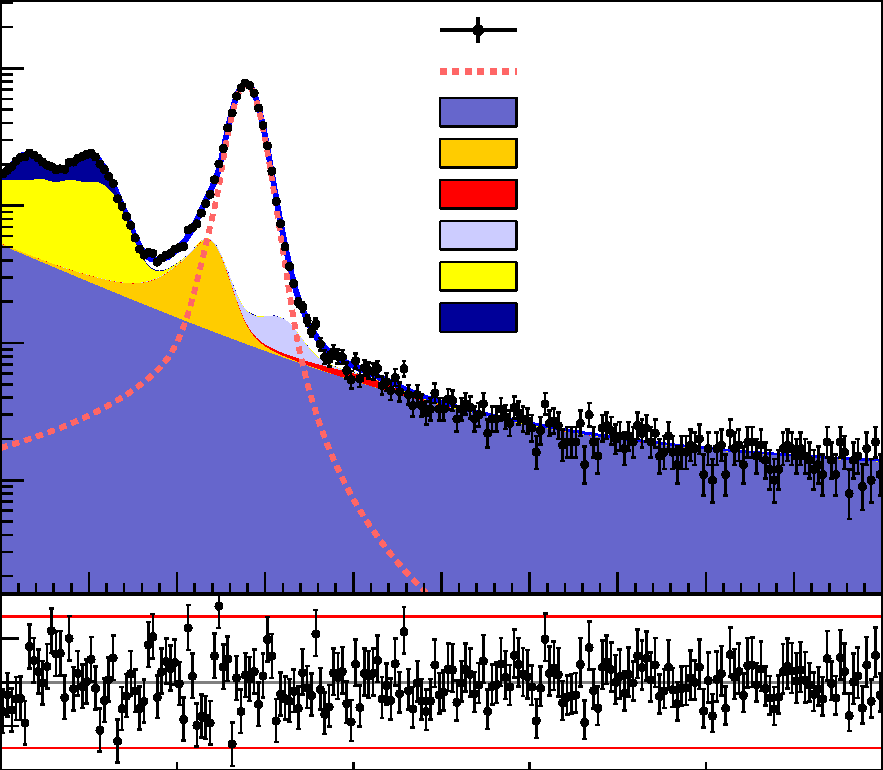
\includegraphics[width=0.9\textwidth]{BsDsK_TD/BdDPi_Fit/mass_Bd2DPi_BeautyMass_up_kpipi_2011}};
            \begin{scope}[x={(image.south east)},y={(image.north west)}]
                \foreach \x/\xtext in {5000, 5200, ..., 6000}
                {
                    \tikzmath{\xpos = (\x - 5000) / 1000;}
                    \node at (\xpos, -0.025) {\(\xtext\)};
                }
                \node[anchor=base east] at (0.005, 0.363) {\(10\)};
                \node[anchor=base east] at (0.005, 0.363+1*.178) {\(10^{2}\)};
                \node[anchor=base east] at (0.005, 0.363+2*.178) {\(10^{3}\)};
                \node[anchor=base east] at (0.005, 0.363+3*.178) {\(10^{4}\)};
                \foreach \p/\ptext in {-2, 0, 2}
                {
                    \tikzmath{\ypos = ((2 + \p) / 2 + 1) * (0.228 / 4);}
                    \node[anchor=east] at (0.005, \ypos) {\(\scriptstyle\ptext\)};
                }
                \node[anchor=east] at (1.0, -0.09) {\({m(\DmpPipm)}~[\si{\MeVcc}]\)};
                \node[rotate=90,anchor=east,inner xsep=0pt,outer xsep=0pt] at (-0.13, 1.0) {\({\text{Candidates}/(\SI{10}{\MeVcc})}\)};
                \node[anchor=east] at (0.26, 0.92) {\large\lhcb};
                % Legend
                {
                    \fontsize{5.5}{6.6}\selectfont
                    \node[anchor=base west] at (0.58, 0.946) {Data};
                    \node[anchor=base west] at (0.58, 0.946 - 1 * 0.0532) {\BdDPi~signal};
                    \node[anchor=base west] at (0.58, 0.946 - 2 * 0.0532) {Combinatorial};
                    \node[anchor=base west] at (0.58, 0.946 - 3 * 0.0532) {\BdDK};
                    \node[anchor=base west] at (0.58, 0.946 - 4 * 0.0532) {\LbLcPi};
                    \node[anchor=base west] at (0.58, 0.946 - 5 * 0.0532) {\BsDsPi};
                    \node[anchor=base west] at (0.58, 0.946 - 6 * 0.0532) {\BdDRho};
                    \node[anchor=base west] at (0.58, 0.946 - 7 * 0.0532) {\BdDstPi};
                }
            \end{scope}
        \end{tikzpicture}
        \caption{\({\sqs = \SI{7}{\TeV}}\), \lhcb~magnet up.}
    \end{subfigure} \hfill%
    \begin{subfigure}{.48\textwidth} \centerfloat
        \begin{tikzpicture}
            \node[anchor=south west,inner sep=0] (image) at (0,0) {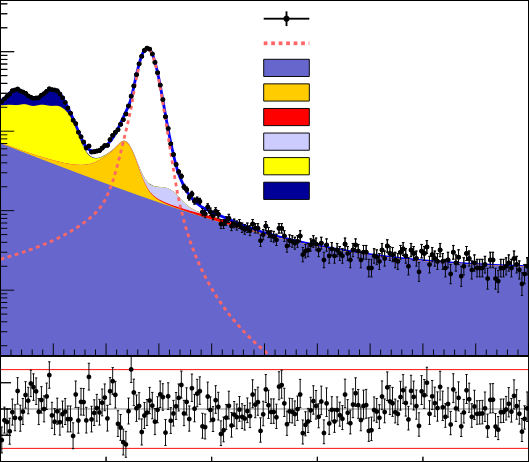
\includegraphics[width=0.9\textwidth]{BsDsK_TD/BdDPi_Fit/mass_Bd2DPi_BeautyMass_down_kpipi_2011}};
            \begin{scope}[x={(image.south east)},y={(image.north west)}]
                \foreach \x/\xtext in {5000, 5200, ..., 6000}
                {
                    \tikzmath{\xpos = (\x - 5000) / 1000;}
                    \node at (\xpos, -0.025) {\(\xtext\)};
                }
                \node[anchor=base east] at (0.005, 0.358) {\(10\)};
                \node[anchor=base east] at (0.005, 0.358+1*.171) {\(10^{2}\)};
                \node[anchor=base east] at (0.005, 0.358+2*.171) {\(10^{3}\)};
                \node[anchor=base east] at (0.005, 0.358+3*.171) {\(10^{4}\)};
                \foreach \p/\ptext in {-2, 0, 2}
                {
                    \tikzmath{\ypos = ((2 + \p) / 2 + 1) * (0.228 / 4);}
                    \node[anchor=east] at (0.005, \ypos) {\(\scriptstyle\ptext\)};
                }
                \node[anchor=east] at (1.0, -0.09) {\({m(\DmpPipm)}~[\si{\MeVcc}]\)};
                \node[rotate=90,anchor=east,inner xsep=0pt,outer xsep=0pt] at (-0.13, 1.0) {\({\text{Candidates}/(\SI{10}{\MeVcc})}\)};
                \node[anchor=east] at (0.26, 0.92) {\large\lhcb};
                % Legend
                {
                    \fontsize{5.5}{6.6}\selectfont
                    \node[anchor=base west] at (0.58, 0.946) {Data};
                    \node[anchor=base west] at (0.58, 0.946 - 1 * 0.0532) {\BdDPi~signal};
                    \node[anchor=base west] at (0.58, 0.946 - 2 * 0.0532) {Combinatorial};
                    \node[anchor=base west] at (0.58, 0.946 - 3 * 0.0532) {\BdDK};
                    \node[anchor=base west] at (0.58, 0.946 - 4 * 0.0532) {\LbLcPi};
                    \node[anchor=base west] at (0.58, 0.946 - 5 * 0.0532) {\BsDsPi};
                    \node[anchor=base west] at (0.58, 0.946 - 6 * 0.0532) {\BdDRho};
                    \node[anchor=base west] at (0.58, 0.946 - 7 * 0.0532) {\BdDstPi};
                }
            \end{scope}
        \end{tikzpicture}
        \caption{\({\sqs = \SI{7}{\TeV}}\), \lhcb~magnet down.}
    \end{subfigure}
    \\[4ex]
    \begin{subfigure}{.48\textwidth} \centerfloat
        \begin{tikzpicture}
            \node[anchor=south west,inner sep=0] (image) at (0,0) {\includegraphics[width=0.9\textwidth]{BsDsK_TD/BdDPi_Fit/mass_Bd2DPi_BeautyMass_up_kpipi_2012}};
            \begin{scope}[x={(image.south east)},y={(image.north west)}]
                \foreach \x/\xtext in {5000, 5200, ..., 6000}
                {
                    \tikzmath{\xpos = (\x - 5000) / 1000;}
                    \node at (\xpos, -0.025) {\(\xtext\)};
                }
                \node[anchor=base east] at (0.005, 0.348) {\(10\)};
                \node[anchor=base east] at (0.005, 0.348 + 1 * .160) {\(10^{2}\)};
                \node[anchor=base east] at (0.005, 0.348 + 2 * .160) {\(10^{3}\)};
                \node[anchor=base east] at (0.005, 0.348 + 3 * .160) {\(10^{4}\)};
                \foreach \p/\ptext in {-2, 0, 2}
                {
                    \tikzmath{\ypos = ((2 + \p) / 2 + 1) * (0.228 / 4);}
                    \node[anchor=east] at (0.005, \ypos) {\(\scriptstyle\ptext\)};
                }
                \node[anchor=east] at (1.0, -0.09) {\({m(\DmpPipm)}~[\si{\MeVcc}]\)};
                \node[rotate=90,anchor=east,inner xsep=0pt,outer xsep=0pt] at (-0.13, 1.0) {\({\text{Candidates}/(\SI{10}{\MeVcc})}\)};
                \node[anchor=east] at (0.26, 0.92) {\large\lhcb};
                % Legend
                {
                    \fontsize{5.5}{6.6}\selectfont
                    \node[anchor=base west] at (0.58, 0.946) {Data};
                    \node[anchor=base west] at (0.58, 0.946 - 1 * 0.0532) {\BdDPi~signal};
                    \node[anchor=base west] at (0.58, 0.946 - 2 * 0.0532) {Combinatorial};
                    \node[anchor=base west] at (0.58, 0.946 - 3 * 0.0532) {\BdDK};
                    \node[anchor=base west] at (0.58, 0.946 - 4 * 0.0532) {\LbLcPi};
                    \node[anchor=base west] at (0.58, 0.946 - 5 * 0.0532) {\BsDsPi};
                    \node[anchor=base west] at (0.58, 0.946 - 6 * 0.0532) {\BdDRho};
                    \node[anchor=base west] at (0.58, 0.946 - 7 * 0.0532) {\BdDstPi};
                }
            \end{scope}
        \end{tikzpicture}
        \caption{\({\sqs = \SI{8}{\TeV}}\), \lhcb~magnet up.}
    \end{subfigure} \hfill%
    \begin{subfigure}{.48\textwidth} \centerfloat
        \begin{tikzpicture}
            \node[anchor=south west,inner sep=0] (image) at (0,0) {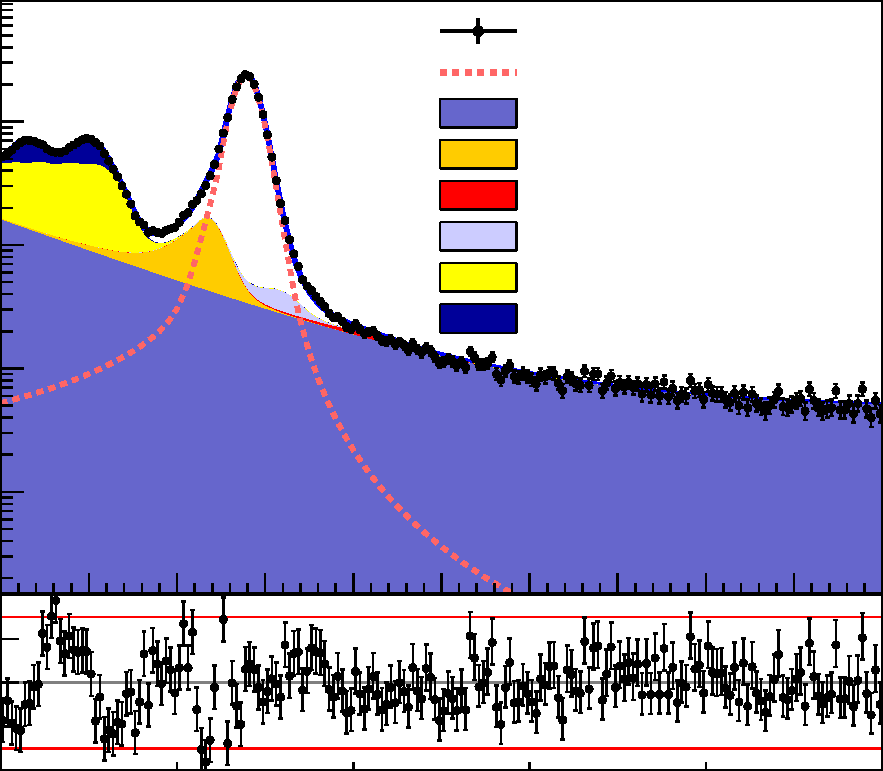
\includegraphics[width=0.9\textwidth]{BsDsK_TD/BdDPi_Fit/mass_Bd2DPi_BeautyMass_down_kpipi_2012}};
            \begin{scope}[x={(image.south east)},y={(image.north west)}]
                \foreach \x/\xtext in {5000, 5200, ..., 6000}
                {
                    \tikzmath{\xpos = (\x - 5000) / 1000;}
                    \node at (\xpos, -0.025) {\(\xtext\)};
                }
                \node[anchor=base east] at (0.005, 0.348) {\(10\)};
                \node[anchor=base east] at (0.005, 0.348 + 1 * .160) {\(10^{2}\)};
                \node[anchor=base east] at (0.005, 0.348 + 2 * .160) {\(10^{3}\)};
                \node[anchor=base east] at (0.005, 0.348 + 3 * .160) {\(10^{4}\)};
                \foreach \p/\ptext in {-2, 0, 2}
                {
                    \tikzmath{\ypos = ((2 + \p) / 2 + 1) * (0.228 / 4);}
                    \node[anchor=east] at (0.005, \ypos) {\(\scriptstyle\ptext\)};
                }
                \node[anchor=east] at (1.0, -0.09) {\({m(\DmpPipm)}~[\si{\MeVcc}]\)};
                \node[rotate=90,anchor=east,inner xsep=0pt,outer xsep=0pt] at (-0.13, 1.0) {\({\text{Candidates}/(\SI{10}{\MeVcc})}\)};
                \node[anchor=east] at (0.26, 0.92) {\large\lhcb};
                % Legend
                {
                    \fontsize{5.5}{6.6}\selectfont
                    \node[anchor=base west] at (0.58, 0.946) {Data};
                    \node[anchor=base west] at (0.58, 0.946 - 1 * 0.0532) {\BdDPi~signal};
                    \node[anchor=base west] at (0.58, 0.946 - 2 * 0.0532) {Combinatorial};
                    \node[anchor=base west] at (0.58, 0.946 - 3 * 0.0532) {\BdDK};
                    \node[anchor=base west] at (0.58, 0.946 - 4 * 0.0532) {\LbLcPi};
                    \node[anchor=base west] at (0.58, 0.946 - 5 * 0.0532) {\BsDsPi};
                    \node[anchor=base west] at (0.58, 0.946 - 6 * 0.0532) {\BdDRho};
                    \node[anchor=base west] at (0.58, 0.946 - 7 * 0.0532) {\BdDstPi};
                }
            \end{scope}
        \end{tikzpicture}
        \caption{\({\sqs = \SI{8}{\TeV}}\), \lhcb~magnet down.}
    \end{subfigure}
    \caption{
        Distributions of the \DmpPipm~invariant mass obtained in the fit to \BdDPi~candidates in data, split by centre-of-mass energy and \lhcb~magnet polarity.
        The solid, blue curve corresponds to the fit described in the text.
        Different contributions to the fit are shown as coloured areas (for backgrounds) or a dashed line (signal), as described in the legend in the figure.}
    \label{fig:BsDsK_TD_BdDPi_Fit}
\end{figure}

From the mass fit, a statistically pure signal sample is extracted using the \sfit~method~\cite{Yuehong_sFit}.
This sample is then compared to the simulated \BdDPi~sample.
This comparison is done in two variables that are relevant to the PID~performance: track momentum and total number of event tracks.

The resulting weights, obtained as the ratio between data and simulation, are shown in \cref{fig:BsDsK_TD_DataMC_Weights}.
In general, they correct for the particle multiplicities, which are too low in simulation.
These weights are applied to each simulated sample used throughout the rest of the analysis.
%
\begin{figure}[htb] \centerfloat
    \hspace*{-1.25cm}
    \fontsize{7}{8.4}\selectfont
    \begin{subfigure}{.45\textwidth} \centerfloat
        \begin{tikzpicture}
            \node[anchor=south west,inner sep=0] (image) at (0,0) {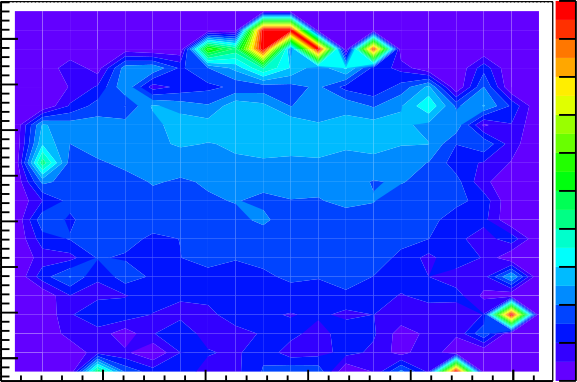
\includegraphics[width=0.9\textwidth]{BsDsK_TD/BdDPi_Fit/datamc_weights_p_nTracks_2011_up_filtered}};
            \begin{scope}[x={(image.south east)},y={(image.north west)}]
                \foreach \x/\xtext in {9, ..., 13}
                {
                    \tikzmath{\xpos = (\x - 9) / 5.62 + 0.18;}
                    \node at (\xpos, -0.045) {\(\xtext\)};
                }
                \foreach \y in {6, ..., 13}
                {
                    \tikzmath{\ypos = (\y - 5.6) / 8.5; \ytext = \y/2;}
                    \node[anchor=base east] at (0.0000, \ypos) {\(\ytext\)};
                }
                \foreach \z in {0, ..., 10}
                {
                    \tikzmath{\ztext = \z/2;}
                    \node[anchor=west] at (1.0, 0.01 + \z/10.15) {\(\pgfmathprintnumber[fixed,precision=1,fixed zerofill=true]{\ztext}\)};
                }
                \node[anchor=east] at (1.0, -0.14) {\(\log(\ptot/(\si{\GeVc}))\)};
                \node[rotate=90,anchor=east,inner xsep=0pt,outer xsep=0pt] at (-0.13, 1.0) {\(\log(\ntr)\)};
            \end{scope}
        \end{tikzpicture}
        \caption{\({\sqs = \SI{7}{\TeV}}\), \lhcb~magnet up.}
    \end{subfigure} \hfill%
    \begin{subfigure}{.45\textwidth} \centerfloat
        \begin{tikzpicture}
            \node[anchor=south west,inner sep=0] (image) at (0,0) {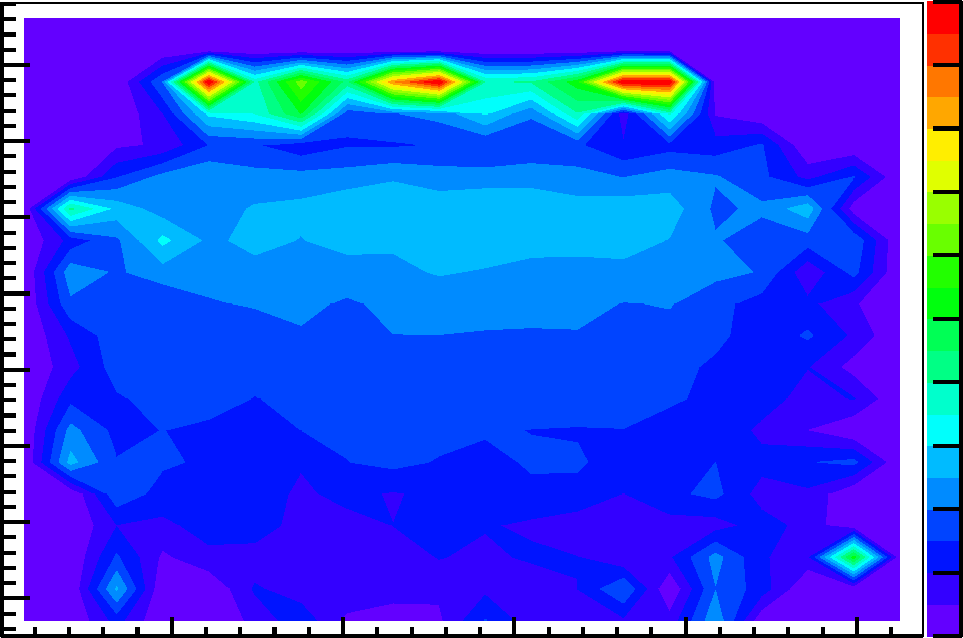
\includegraphics[width=0.9\textwidth]{BsDsK_TD/BdDPi_Fit/datamc_weights_p_nTracks_2011_dw_filtered}};
            \begin{scope}[x={(image.south east)},y={(image.north west)}]
                \foreach \x/\xtext in {9, ..., 13}
                {
                    \tikzmath{\xpos = (\x - 9) / 5.62 + 0.18;}
                    \node at (\xpos, -0.045) {\(\xtext\)};
                }
                \foreach \y in {6, ..., 13}
                {
                    \tikzmath{\ypos = (\y - 5.6) / 8.5; \ytext = \y/2;}
                    \node[anchor=base east] at (0.0000, \ypos) {\(\ytext\)};
                }
                \foreach \z in {0, ..., 10}
                {
                    \tikzmath{\ztext = \z/2;}
                    \node[anchor=west] at (1.0, 0.01 + \z/10.15) {\(\pgfmathprintnumber[fixed,precision=1,fixed zerofill=true]{\ztext}\)};
                }
                \node[anchor=east] at (1.0, -0.14) {\(\log(\ptot/(\si{\GeVc}))\)};
                \node[rotate=90,anchor=east,inner xsep=0pt,outer xsep=0pt] at (-0.13, 1.0) {\(\log(\ntr)\)};
            \end{scope}
        \end{tikzpicture}
        \caption{\({\sqs = \SI{7}{\TeV}}\), \lhcb~magnet down.}
    \end{subfigure}
    \\[4ex]
    \hspace*{-1.25cm}
    \begin{subfigure}{.45\textwidth} \centerfloat
        \begin{tikzpicture}
            \node[anchor=south west,inner sep=0] (image) at (0,0) {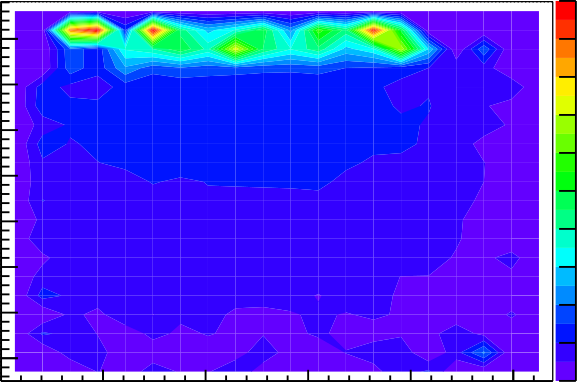
\includegraphics[width=0.9\textwidth]{BsDsK_TD/BdDPi_Fit/datamc_weights_p_nTracks_2012_up_filtered}};
            \begin{scope}[x={(image.south east)},y={(image.north west)}]
                \foreach \x/\xtext in {9, ..., 13}
                {
                    \tikzmath{\xpos = (\x - 9) / 5.62 + 0.18;}
                    \node at (\xpos, -0.045) {\(\xtext\)};
                }
                \foreach \y in {6, ..., 13}
                {
                    \tikzmath{\ypos = (\y - 5.6) / 8.5; \ytext = \y/2;}
                    \node[anchor=base east] at (0.0000, \ypos) {\(\ytext\)};
                }
                \foreach \z/\ztext in {0, ..., 10}
                    \node[anchor=west] at (1.0, 0.01 + \z/10.15) {\(\ztext\)};
                \node[anchor=east] at (1.0, -0.14) {\(\log(\ptot/(\si{\GeVc}))\)};
                \node[rotate=90,anchor=east,inner xsep=0pt,outer xsep=0pt] at (-0.13, 1.0) {\(\log(\ntr)\)};
            \end{scope}
        \end{tikzpicture}
        \caption{\({\sqs = \SI{8}{\TeV}}\), \lhcb~magnet up.}
    \end{subfigure} \hfill%
    \begin{subfigure}{.45\textwidth} \centerfloat
        \begin{tikzpicture}
            \node[anchor=south west,inner sep=0] (image) at (0,0) {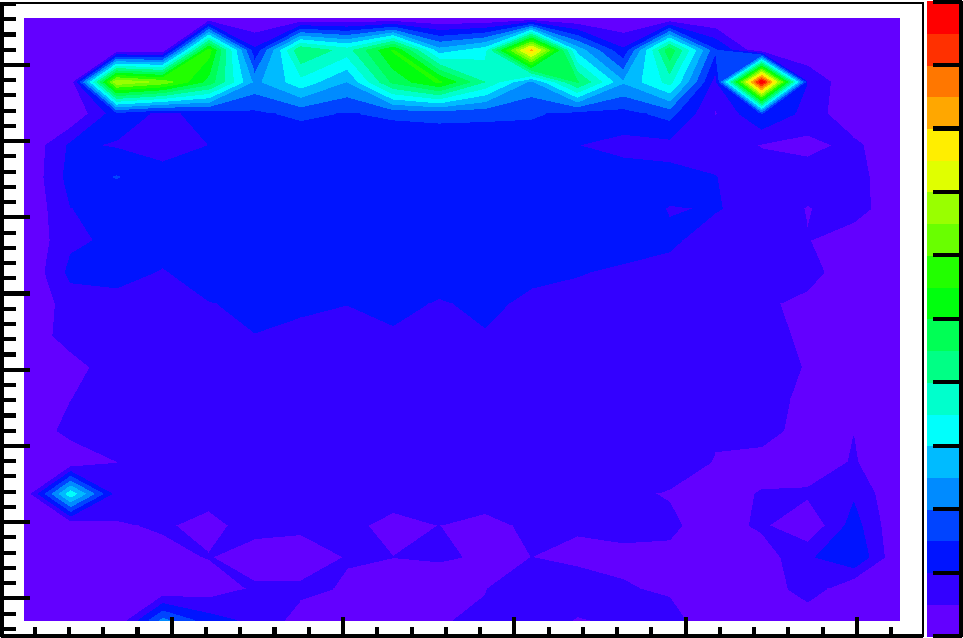
\includegraphics[width=0.9\textwidth]{BsDsK_TD/BdDPi_Fit/datamc_weights_p_nTracks_2012_dw_filtered}};
            \begin{scope}[x={(image.south east)},y={(image.north west)}]
                \foreach \x/\xtext in {9, ..., 13}
                {
                    \tikzmath{\xpos = (\x - 9) / 5.62 + 0.18;}
                    \node at (\xpos, -0.045) {\(\xtext\)};
                }
                \foreach \y in {6, ..., 13}
                {
                    \tikzmath{\ypos = (\y - 5.6) / 8.5; \ytext = \y/2;}
                    \node[anchor=base east] at (0.0000, \ypos) {\(\ytext\)};
                }
                \foreach \z/\ztext in {0, ..., 10}
                    \node[anchor=west] at (1.0, 0.01 + \z/10.15) {\(\ztext\)};
                \node[anchor=east] at (1.0, -0.14) {\(\log(\ptot/(\si{\GeVc}))\)};
                \node[rotate=90,anchor=east,inner xsep=0pt,outer xsep=0pt] at (-0.13, 1.0) {\(\log(\ntr)\)};
            \end{scope}
        \end{tikzpicture}
        \caption{\({\sqs = \SI{8}{\TeV}}\), \lhcb~magnet down.}
    \end{subfigure}
    \caption{
        Data/simulation ratios as obtained from the \BdDPi~fits as a function of track momentum~\ptot and number of tracks in the event~\ntr, split by centre-of-mass energy and \lhcb~magnet polarity.
        Differences between the ratios for different \lhcb~magnet polarities are possibly due to differences in the crossing angle of the proton beams.}
    \label{fig:BsDsK_TD_DataMC_Weights}
\end{figure}

\clearpage
\section{Signal extraction} \label{sec:BsDsK_TD_MD_Fit}

\subsection{Motivation} \label{sec:BsDsK_TD_MD_Fit_Motivation}

A pure sample of \BsDsK~events is required to extract the time-dependent \CP~observables.
This sample is obtained by fitting the data, including information on the various backgrounds present, and statistically subtracting the background.
In addition, a kinematically similar sample of \BsDsPi~events is extracted in the same way, and used for flavour tagging and decay-time acceptance calibration (see \cref{chp:BsDsK_TD}).

To identify signal events, three variables with good discriminating properties for the various event categories are selected: the \Bs~candidate mass, the \Dsmp~candidate mass, and the PID~information of the companion track~(\({\log|\dllkpi|}\)).
These three variables are simultaneously fitted using a multivariate, unbinned extended maximum likelihood fit.
Two separate fits are performed for the \BsDsPi~and \BsDsK~samples, which are split by~\dllkpi as specified in \cref{tab:BsDsK_TD_Selection}: \({< \num{0}}\)~for the pion companion, and \({> \num{5}}\)~for the kaon.
In the following sections, the definitions of signal, background and combinatorial shapes in each of the three variables are given.
Both fits are set up similarly, with some differences -- most notably in the treatment of backgrounds -- as discussed below.

\subsection{PID reweighting} \label{sec:BsDsK_TD_MD_PID_Reweighting}

The shapes of the mass distributions for the \Bs~and \Dsmp~candidates are readily extracted from simulated samples, but for the companion \dllkpi~distributions, the description in simulation is inadequate, and a more involved procedure is employed.
The starting point is the \dllkpi~shape for a control mode from data, namely \DstarDPi~for pure pion and kaon samples, and \Lzppi~for a pure proton sample~\cite{Powell:1322666}.
The background in each of these samples is subtracted using statistical weights, and the relevant \dllkpi~requirement (\({< \num{0}}\)~or \({> \num{5}}\))~is applied.
The sample is subsequently weighted to match the momentum and rapidity distributions of companion tracks from corresponding \Bs~decays.
These simulated samples are first weighted using the corrections obtained with the procedure from \cref{sec:TD_DsK_Simulation}, after which the data calibration sample is weighted to match the track momentum and the number of tracks in the event (or rather, the logarithm of those variables).
For \BsDsK, however, the shape of the track momentum does not yield well-behaved \dllkpi~shapes, and the track transverse momentum,~\({\log(\pt)}\), is used instead.
This weighting is performed separately for each centre-of-mass energy and magnet polarity, after which they are combined in ratios corresponding to the amount of luminosity in the data.
For each variable, twenty bins are used (\num{400}~bins total).
Several binning schemes have been examined, and the difference between the resulting distributions is found to be negligible.

Correlations between the \Bs~invariant mass, \Dsmp~invariant mass, and companion~\dllkpi have been studied to ensure that the extracted weights are correct.
Correlations between these variables and the decay time and per-event decay-time error, are also checked.
To investigate the effects of such correlations, large samples of background events have been generated using a phase-space generator.
Correlations between the fit variables and the decay-time variables are generally found to be of the order~\SI{5}{\percent}.
These correlations are slightly larger in some channels, up to about~\SI{25}{\percent} in a few of them.
All these correlations are accounted for in the systematic uncertainties by performing pseudo-experiments (see \cref{sec:BsDsK_TD_Syst}).

\subsection{Signal shape}

The signal shapes of the \Bs~and \Dsmp~invariant mass distributions are parameterised using a DCB~shape (see \cref{sec:MassFits_Signal}) with shared mean, with the fraction between the Gaussian distributions fixed to~\num{0.5}.
The tail parameters are obtained by fitting the corresponding simulated sample.
This is done separately for each of the five \Dsmp~final states, for both~\BsDsPi and~\BsDsK, and for both the \Bs~and \Dsmp~invariant masses (twenty fits total).
The results of those fits are shown in \cref{fig:BsDsK_TD_Signal_Shape_Results,tab:BsDsK_TD_Signal_Shape_Results}.
In the~PDF used in the multivariate fit, the mean is left floating to account for slight differences between data and simulation, and the mass resolution~\DCBs is scaled by a mass resolution scale factor~\(R\).
This parameter is shared among all \Dsmp~modes but separate for the \Bs~and \Dsmp~signal shapes, yielding two parameters \RBs~and \RDs~for each multivariate fit.

To obtain a shape for the \dllkpi~distribution of the companion candidates, the procedure described in \cref{sec:BsDsK_TD_MD_PID_Reweighting} is applied.
A calibration sample of the respective type of companion particle (pion or kaon) is taken, and reweighted to match the kinematics of the signal decay, as determined from simulation.
%
\begin{figure}[hp] \centerfloat
    \fontsize{7}{8.4}\selectfont
    \begin{subfigure}{.44\textwidth} \centerfloat
        \begin{tikzpicture}
            \node[anchor=south west,inner sep=0] (image) at (0,0) {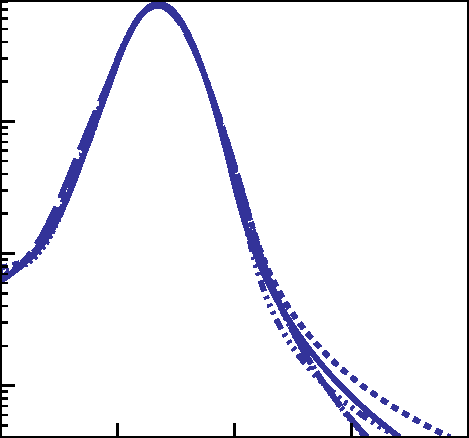
\includegraphics[width=0.9\textwidth]{BsDsK_TD/Signal_Templates/BsDsK_BsMass}};
            \begin{scope}[x={(image.south east)},y={(image.north west)}]
                \foreach \x/\xtext in {5300, 5350, ..., 5500}
                {
                    \tikzmath{\xpos = (\x - 5300) / 200;}
                    \node at (\xpos, -0.025) {\(\xtext\)};
                }
                \node[anchor=base east] at (0.005, 0.107) {\num{e-4}};
                \node[anchor=base east] at (0.005, 0.107 + 1 * 0.301) {\num{e-3}};
                \node[anchor=base east] at (0.005, 0.107 + 2 * 0.301) {\num{e-2}};
                \node[anchor=east] at (1.0, -0.09) {\({m(\DsmpKpm)}~[\si{\MeVcc}]\)};
                \node[rotate=90,anchor=east,inner xsep=0pt,outer xsep=0pt] at (-0.13, 1.0) {PDF};
                \node[anchor=east] at (0.91, 0.92) {\large\lhcb};
            \end{scope}
        \end{tikzpicture}
        \caption{\Bs~mass.}
    \end{subfigure} \hfill%
    \begin{subfigure}{.44\textwidth} \centerfloat
        \begin{tikzpicture}
            \node[anchor=south west,inner sep=0] (image) at (0,0) {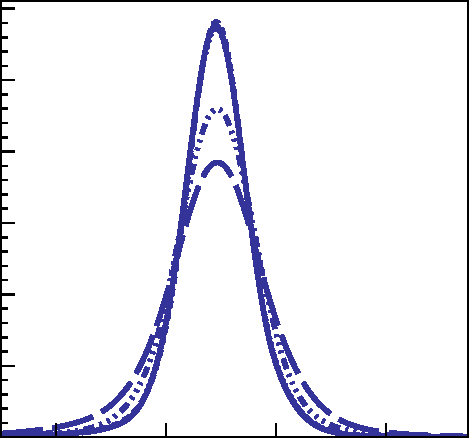
\includegraphics[width=0.9\textwidth]{BsDsK_TD/Signal_Templates/BsDsK_DsMass}};
            \begin{scope}[x={(image.south east)},y={(image.north west)}]
                \foreach \x/\xtext in {1940, 1960, ..., 2000}
                {
                    \tikzmath{\xpos = (\x - 1940) / (2000 - 1940) * (0.822 - 0.12) + 0.12;}
                    \node at (\xpos, -0.025) {\(\xtext\)};
                }
                \node[anchor=east] at (0.005, 0.) {\num{0}};
                \foreach \y in {1, ..., 6}
                {
                    \tikzmath{\ypos = \y / 6.13; \ytext = \y / 100;}
                    \node[anchor=east] at (0.005, \ypos) {\pgfmathprintnumber[fixed,precision=2,fixed zerofill=true]{\ytext}};
                }
                \node[anchor=east] at (1.0, -0.09) {\({m(\Dsmp)}~[\si{\MeVcc}]\)};
                \node[rotate=90,anchor=east,inner xsep=0pt,outer xsep=0pt] at (-0.14, 1.0) {PDF};
                \node[anchor=east] at (0.91, 0.92) {\large\lhcb};
            \end{scope}
        \end{tikzpicture}
        \caption{\Dsmp~mass.}
    \end{subfigure} \vspace{2ex}
    \begin{subfigure}{.70\textwidth} \centerfloat
        \begin{tikzpicture}[scale=0.9, every node/.style={scale=0.9}]
            \node[anchor=south west,inner sep=0] (image) at (0,0) {\includegraphics[width=0.9\textwidth]{BsDsK_TD/Signal_Templates/BsDsPi_CompDLLkpi}};
            \begin{scope}[x={(image.south east)},y={(image.north west)}]
                \node at (0.163, -0.025) {\num{-5}};
                \node at (0.583, -0.025) {\num{ 0}};
                \node at (1.  , -0.025) {\num{ 5}};
                \node[anchor=east] at (0.005, 0.) {\num{0}};
                \foreach \y in {1, ..., 5}
                {
                    \tikzmath{\ypos = \y / 5.07; \ytext = \y / 100;}
                    \node[anchor=east] at (0.005, \ypos) {\pgfmathprintnumber[fixed,precision=2,fixed zerofill=true]{\ytext}};
                }
                % Legend
                {
                    \node[anchor=base west] at (0.145, 0.79) {\DsmNonRes};
                    \node[anchor=base west] at (0.145, 0.79 - 1 * 0.0692) {\DsmPhiPi};
                    \node[anchor=base west] at (0.145, 0.79 - 2 * 0.0692) {\DsmKstK};
                    \node[anchor=base west] at (0.145, 0.79 - 3 * 0.0692) {\DsmKPiPi};
                    \node[anchor=base west] at (0.145, 0.79 - 4 * 0.0692) {\DsmPiPiPi};
                }
                \node[anchor=east] at (1.0, -0.09) {\({\log(-\dllkpi)}\)};
                \node[rotate=90,anchor=east,inner xsep=0pt,outer xsep=0pt] at (-0.09, 1.0) {PDF};
                \node[anchor=west] at (0.06, 0.92) {\large\lhcb};
            \end{scope}
        \end{tikzpicture}
        \caption{Companion~\dllkpi for pion companions.}
    \end{subfigure} \vspace{2ex}
    \begin{subfigure}{.70\textwidth} \centerfloat
        \begin{tikzpicture}[scale=0.9, every node/.style={scale=0.9}]
            \node[anchor=south west,inner sep=0] (image) at (0,0) {\includegraphics[width=0.9\textwidth]{BsDsK_TD/Signal_Templates/BsDsK_CompDLLkpi}};
            \begin{scope}[x={(image.south east)},y={(image.north west)}]
                \node at (0.117, -0.025) {\num{2}};
                \node at (0.411, -0.025) {\num{3}};
                \node at (0.704, -0.025) {\num{4}};
                \node at (1.   , -0.025) {\num{5}};
                \node[anchor=east] at (0.005, 0.) {\num{0}};
                \foreach \y in {2, 4, ..., 22}
                {
                    \tikzmath{\ypos = \y / 22.7; \ytext = \y / 1000;}
                    \node[anchor=east] at (0.005, \ypos) {\pgfmathprintnumber[fixed,precision=3,fixed zerofill=true]{\ytext}};
                }
                \node[anchor=east] at (1.0, -0.09) {\({\log(\dllkpi)}\)};
                \node[rotate=90,anchor=east,inner xsep=0pt,outer xsep=0pt] at (-0.125, 1.0) {PDF};
                \node[anchor=east] at (0.91, 0.92) {\large\lhcb};
            \end{scope}
        \end{tikzpicture}
        \caption{Companion~\dllkpi for kaon companions.}
    \end{subfigure}
    \caption{
        Signal shape~PDF parameterisations of the \Bs~and \Dsmp~invariant mass distributions for \BsDsK~candidates, and the \dllkpi~for both \BsDsPi~and \BsDsK~companion tracks.
        The mass shapes for \BsDsPi~(not shown) are very similar to their \BsDsK~counterparts.
        Note that the companion~\dllkpi templates are functions of~\({\log\left(\left|\dllkpi\right|\right)}\), with~\({\dllkpi < 0}\) for~\BsDsPi and~\({\dllkpi > 5}\) for~\BsDsK.}
    \label{fig:BsDsK_TD_Signal_Shape_Results}
\end{figure}

\begin{landscape}
\begin{table}[hp] \centerfloat
    \caption{
        Parameters of the double Crystal~Ball parameterisations describing the signal \Bs~and \Dsmp~shapes of the two signal samples, obtained from fits to respective simulated samples.}
    \label{tab:BsDsK_TD_Signal_Shape_Results}
    \rowcolors{4}{tableshade}{}
    \sisetup{table-number-alignment=right}
    \scriptsize
    \begin{tabular}{lS[table-format=4.2(2)]*{2}{S[table-format=2.2(2)]}S[table-format=+1.2(2)]S[table-format=1.2(2)]*{2}{S[table-format=2.2(2)]}}
        \toprule
        Mode        & \DCBmu          & \DCBsL        & \DCBsR        & \DCBaL        & \DCBaR       & \DCBnL            & \DCBnR \tabularnewline
                    & \si{\MeVcc}     & \si{\MeVcc}   & \si{\MeVcc}   &               &              &                   &        \tabularnewline
        \midrule
        \multicolumn{8}{l}{\BsDsPi,~\Bs~signal shape} \tabularnewline
        \midrule
        \DsmPhiPi   & 5367.11 +- 0.05 & 18.39 +- 0.16 & 11.43 +- 0.07 & -2.19 +- 0.03 & 2.25 +- 0.11 &  2.37 +- 0.09     &  0.42 +-  0.13 \tabularnewline
        \DsmKstK    & 5367.01 +- 0.05 & 12.39 +- 0.17 & 16.03 +- 0.33 & -1.83 +- 0.07 & 1.26 +- 0.06 &  2.82 +- 0.21     &  5.12 +-  1.54 \tabularnewline
        \DsmNonRes  & 5367.19 +- 0.08 & 17.48 +- 0.31 & 11.54 +- 0.12 & -2.18 +- 0.06 & 2.15 +- 0.19 &  2.54 +- 0.17     &  0.52 +-  0.25 \tabularnewline
        \DsmKPiPi   & 5366.93 +- 0.08 & 18.01 +- 0.26 & 11.51 +- 0.14 & -2.19 +- 0.07 & 2.07 +- 0.13 &  2.68 +- 0.23     &  0.52 +-  0.18 \tabularnewline
        \DsmPiPiPi  & 5366.74 +- 0.07 & 18.79 +- 0.24 & 11.79 +- 0.11 & -2.27 +- 0.07 & 2.07 +- 0.12 &  2.50 +- 0.21     &  0.52 +-  0.1  \tabularnewline
        \hiderowcolors \midrule
        \multicolumn{8}{l}{\BsDsPi,~\Dsm~signal shape} \tabularnewline
        \showrowcolors \midrule
        \DsmPhiPi   & 1968.95 +- 0.02 &  5.37 +- 0.11 &  5.89 +- 0.15 & -1.11 +- 0.04 & 1.14 +- 0.03 &  8.69 +- 1.93     &  5.86 +-  0.58 \tabularnewline
        \DsmKstK    & 1969.00 +- 0.03 &  5.63 +- 0.18 &  6.18 +- 0.26 & -1.18 +- 0.07 & 1.26 +- 0.04 & 11.38 +- 5.21     &  5.89 +-  1.02 \tabularnewline
        \DsmNonRes  & 1968.99 +- 0.04 &  5.94 +- 0.30 &  5.50 +- 0.23 & -1.16 +- 0.05 & 1.28 +- 0.09 & 16.05 +- 8.43     &  3.69 +-  0.98 \tabularnewline
        \DsmKPiPi   & 1969.07 +- 0.05 &  6.69 +- 0.22 &  7.49 +- 0.17 & -1.17 +- 0.03 & 1.02 +- 0.09 & \centercell{10.0} & 10.41 +-  8.45 \tabularnewline
        \DsmPiPiPi  & 1969.12 +- 0.05 &  8.52 +- 0.60 &  8.62 +- 0.63 & -1.07 +- 0.13 & 0.98 +- 0.15 & \centercell{20.0} &  5.37 +-  5.31 \tabularnewline
        \hiderowcolors \midrule
        \multicolumn{8}{l}{\BsDsK,~\Bs~signal shape} \tabularnewline
        \showrowcolors \midrule
        \DsmpPhiPi  & 5367.33 +- 0.05 & 16.29 +- 0.21 & 10.93 +- 0.09 & -2.17 +- 0.05 & 2.07 +- 0.13 &  2.97 +- 0.17     &  0.89 +-  0.23 \tabularnewline
        \DsmpKstK   & 5367.19 +- 0.05 & 16.15 +- 0.19 & 10.94 +- 0.10 & -2.29 +- 0.06 & 2.18 +- 0.13 &  3.10 +- 0.24     &  0.72 +-  0.20 \tabularnewline
        \DsmpNonRes & 5367.31 +- 0.07 & 16.37 +- 0.28 & 10.87 +- 0.14 & -2.26 +- 0.07 & 2.35 +- 0.21 &  2.83 +- 0.24     &  0.41 +-  0.26 \tabularnewline
        \DsmpKPiPi  & 5367.03 +- 0.07 & 16.24 +- 0.26 & 10.96 +- 0.16 & -2.26 +- 0.10 & 2.15 +- 0.13 &  3.21 +- 0.41     &  0.69 +-  0.20 \tabularnewline
        \DsmpPiPiPi & 5366.98 +- 0.06 & 16.91 +- 0.22 & 11.15 +- 0.11 & -2.26 +- 0.07 & 2.01 +- 0.13 &  3.11 +- 0.27     &  0.89 +-  0.22 \tabularnewline
        \hiderowcolors \midrule
        \multicolumn{8}{l}{\BsDsK,~\Dsmp~signal shape} \tabularnewline
        \showrowcolors \midrule
        \DsmpPhiPi  & 1968.91 +- 0.03 &  5.34 +- 0.13 &  5.73 +- 0.16 & -1.09 +- 0.04 & 1.16 +- 0.03 & 10.18 +- 2.71     &  5.72 +-  0.77 \tabularnewline
        \DsmpKstK   & 1969.04 +- 0.03 &  5.73 +- 0.22 &  5.96 +- 0.24 & -1.24 +- 0.05 & 1.23 +- 0.04 & 10.19 +- 3.20     &  6.20 +-  1.50 \tabularnewline
        \DsmpNonRes & 1968.97 +- 0.03 &  5.29 +- 0.13 &  6.11 +- 0.18 & -1.20 +- 0.05 & 1.22 +- 0.05 &  8.17 +- 1.79     &  5.24 +-  0.97 \tabularnewline
        \DsmpKPiPi  & 1968.97 +- 0.06 &  6.55 +- 0.16 &  7.62 +- 0.16 & -1.19 +- 0.03 & 1.11 +- 0.08 & \centercell{10.0} &  8.84 +-  4.61 \tabularnewline
        \DsmpPiPiPi & 1969.19 +- 0.05 &  7.93 +- 0.11 &  8.68 +- 0.14 & -1.04 +- 0.02 & 0.82 +- 0.02 & \centercell{20.0} & 48.4  +- 61.2  \tabularnewline
        \bottomrule
    \end{tabular}
\end{table}
\end{landscape}

\subsection{Physics backgrounds}

Three types of so-called physics backgrounds are distinguished: fully reconstructed backgrounds, misidentified backgrounds, and partially reconstructed backgrounds.
The relevant backgrounds for each final state are listed in \cref{tab:BsDsK_TD_Backgrounds}, and their treatment in the multivariate fit is described below.
%
\begin{table}[hp] \centerfloat
    \caption{
        Physics backgrounds that appear in the data, per final state, and their properties.
        Charge conjugation is implied.
        The backgrounds labelled as having misidentified \Dsm~daughters each have one misidentified daughter in the \KmKPi~modes, and two in the \KpPimPim~mode (due to the charges of the hadrons, misidentification between~\DsmKPiPi and~\DmKPiPi is not possible if only one particle is misidentified).
        The five columns labelled with \Dsm~modes represent the fixed yields set for those backgrounds in that mode.
        Empty cells imply the yield is not constrained.}
    \label{tab:BsDsK_TD_Backgrounds}
    \rowcolors{2}{tableshade}{}
    \sisetup{tight-spacing=true, table-number-alignment=right, table-column-width=1.7em}
    \begin{tabular}{l*{4}{l}*{5}{S}}
        Process & \crot{60}{Fully reconstructed} & \crot{60}{Misidentified companion} & \crot{60}{Misidentified \Dsm~daughter(s)} & \crot{60}{Partially reconstructed} & \crot{60}{\DsmNonRes} & \crot{60}{\DsmPhiPi} & \crot{60}{\DsmKstK} & \crot{60}{\DsmKPiPi} & \crot{60}{\DsmPiPiPi} \tabularnewline
        \toprule
        \multicolumn{10}{l}{\BsDsPi} \tabularnewline
        \midrule
        \quad\BdDsPi & \chk & & & & & & & & \tabularnewline
        \quad\BsDsK & & \chk & & & 116 & 262 & 163 & 66 & 158 \tabularnewline
        \quad\BdDPi & & & \chk & & 151 & 11.3 & 31.7 & 30.2 & 0 \tabularnewline
        \quad\LbLcPi & & & \chk & & 482 & 95.4 & 154 & 4.4 & 0 \tabularnewline
        \quad\BsDsstPi & & & & \chk & & & & & \tabularnewline
        \midrule
        \multicolumn{10}{l}{\BsDsK} \tabularnewline
        \midrule
        \quad\BdDsK & \chk & & & & & & & & \tabularnewline
        \quad\BsDsPi & & \chk & & & & & & & \tabularnewline
        \quad\LbDsP & & \chk & & & & & & & \tabularnewline
        \quad\BdDK & & & \chk & & 11.5 & 0.9 & 2.5 & 0 & 0 \tabularnewline
        \quad\BdDPi & & \chk & \chk & & 4.9 & 0.3 & 1.0 & 0 & 0 \tabularnewline
        \quad\LbLcK & & & \chk & & 37.6 & 7.4 & 12.1 & 0 & 0 \tabularnewline
        \quad\LbLcPi & & \chk & \chk & & 15.6 & 3.1 & 5.0 & 0 & 0 \tabularnewline
        \quad\BsDsstPi & & \chk & & \chk & & & & & \tabularnewline
        \quad\BsDsRho & & \chk & & \chk & & & & &\tabularnewline
        \quad\LbDsstP & & \chk & & \chk & & & & &\tabularnewline
        \bottomrule
    \end{tabular}
\end{table}

First of all, there are two fully reconstructed backgrounds, namely the \Bd~counterparts of the signal decays:~\BdDsPi and~\BdDsK.
The \Bs~invariant mass shapes use the same DCB~shape as the \Bs~signal, except for a negative \({\Bd-\Bs}\)~mass difference of~\SI{87}{\MeVcc}~\cite{PDG}.
The mass resolution scale factor~\(R\) is also corrected, with the ratio corresponding to the mass width ratio measured between simulated samples of \BdDsPi (\BdDsK)~and \BsDsPi (\BsDsK)~decays.
The shapes in the \Dsmp~invariant mass and companion~\dllkpi are identical to those used for the signal.

All other physics backgrounds are modelled by taking the reconstructed \Bs~invariant mass shape from corresponding simulated samples and parameterising them using kernel estimation (see \cref{sec:methods_KernelEstimation}).
For the \Dsm~invariant mass, the signal parameterisation is used for the processes that contain a~\DsorDssm, and kernel estimation distributions are taken from corresponding simulated samples in case of a misidentified~\Dm or~\Lc.
The companion~\dllkpi distribution is obtained by applying the reweighting procedure outlined in \cref{sec:BsDsK_TD_MD_PID_Reweighting} to the respective simulated sample.

For several backgrounds it is sensible to fix their yields, as they can be accurately estimated from relative branching fractions and selection efficiencies.
These backgrounds with fixed yields are listed in \cref{tab:BsDsK_TD_Backgrounds}, split per \Dsm~mode.

Three backgrounds are constrained in the \BsDsPi~multivariate fit.
Firstly, the yield of the misidentified background~\BsDsK is fixed as a fraction of the signal yield, accounting for the relative branching fractions and the efficiency of that decay under the requirement of companion \({\dllkpi < \num{0}}\).
Secondly, the misidentified \BdDPi~yield is estimated from the signal \BdDPi~fit described in \cref{sec:TD_DsK_Simulation_Corrections}, corrected for the relative selection efficiency (as determined by applying the selections to simulation samples) and the misidentification rate.
The latter is calculated by weighting the momentum spectrum of simulated \BdDPi~samples to the misidentification rate as determined from \DstarDPi~data.
The third and last constrained yield is that of \LbLcPi, which is determined by a separate fit of the \BsDsPi~candidates, in the \LcPi~mass hypothesis.
In this fit, the \Lc~veto (see \cref{sec:BsDsK_TD_Selection_Signal}) is omitted, and instead the \PKPi~combination is required to fall in a \SI{30}{\MeVcc}~window around the known \Lc~mass of~\SI{2286.5}{\MeVcc}~\cite{PDG}.
The track now reconstructed as a proton is required to have~\({\dllppi > \num{0}}\) and~\({\dllkp < \num{5}}\).
The fit consists of the same DCB~shape for the signal, and a single exponential representing background.
This fit is performed separately for each of the four \Dsm~modes under which it appears (see \cref{tab:BsDsK_TD_Backgrounds}) and separately for~\({\sqs = \SI{7}{\TeV}}\) and~\(\SI{8}{\TeV}\), for a total of eight fits.
The yield obtained from these fits is used as the \LbLcPi~yield under the \DsmPip~mass hypothesis, after correcting for the difference in efficiency due to the different selection procedure.
Note that the yields for the backgrounds \BdDPi~and \LbLcPi~are not computed for the mode~\DsmPiPiPi, and instead omitted in that fit, as they are found to be negligible there.

In the \BsDsK~fit, four background channels have their yields fixed: \BdDK,~\BdDPi,~\LbLcK, and~\LbLcPi.
Each of these yields is taken from the method described above, except that they are corrected for the efficiency of the different companion \dllkpi~requirement (\({> \num{5}}\)~rather than~\({< \num{0}}\)), and the yields of \BdDK~and \LbLcK~are corrected for the difference in branching fraction.
All these backgrounds are negligible, and therefore omitted from the fit, in the \DsmKPiPi~and \DsmPiPiPi~modes.
The yields of the other backgrounds are floating, but constrained, firstly by requiring the yields of the similar backgrounds \BsDsstPi~and \BsDsRho~to be equal, and secondly by fixing the \LbDsstP~yield to~\(\sfrac{1}{3}\) of the \LbDsP~yield.

\subsection{Combinatorial background}

Though the~BDT is specifically trained to suppress combinatorial background while retaining the signal, some combinatorial events remain present in the sample.
These nonphysical combinations of random tracks must be modelled to obtain a good fit.
They can be categorised into two types: real \Dsm~mesons paired with a random track, and random four-track combinations.
To examine their shapes, the upper \Bs~invariant mass sideband,~\SI[parse-numbers=false]{[\num{5800}, \num{7000}]}{\MeVcc}, is inspected, as it contains no physical background processes.
From that sample it can be seen that the combinatorial background can be modelled with an exponential function plus a constant offset.
The exponential parameter and the fraction between those two functions is left floating in the fit.
The resulting shape of the combinatorial background is shown in \cref{fig:BsDsK_TD_Comb_Shape_Results}.
For the modes~\DsmKPiPi and~\DsmPiPiPi in the \BsDsK~multivariate fit a single exponential is found to be a sufficient description of the combinatorial background.

To determine the \Dsm~invariant mass shape of the combinatorial component, the same upper \Bs~mass sideband is investigated.
There is a clear peak of real \Dsm~mesons in the \Dsm~invariant mass, as well as a background of random three-track combinations (see \cref{fig:BsDsK_TD_Comb_Shape_Results}).
These are modelled with a DCB~shape for the \Dsm~mass peak, of which the parameters are fixed to those determined earlier from the fit to simulation, and an exponential for the rest, of which the slope is left floating in the multivariate fit.
The fraction between these two components is also a free parameter.

Finally, the companion~\dllkpi shape receives contributions from all types of particles present in the combinatorial background: pions,~kaons, and~protons.
The shapes of these distributions are again obtained by kinematically reweighting those from \Dstar~and \Lz~samples.
To be able to perform this reweighting, the kinematics of the combinatorial companion particle must be extrapolated from the sideband region into the signal region.
This is done by dividing the upper mass sideband~\({m(\Bs) \in \SI[parse-numbers=false]{[\num{5600}, \num{5800}]}{\MeVcc}}\) in ten bins of~\({m(\Bs)}\), and for each bin fitting a Landau distribution to both the transverse momentum as well as the total number of tracks.
The parameters of these Landau~distributions are then extrapolated from the upper mass sideband into the signal region, estimating the behaviour of combinatorial background in that region.
The calibration samples are weighted according to these extrapolated kinematics, from which the \dllkpi~shapes for the three types of hadron are extracted.
In the \BsDsPi~multivariate fit, only the pion and kaon shapes are used, as the pion-proton misidentification rate is small.
The fraction between these shapes is a free parameter.
In the \BsDsK~fit, the \dllkpi~shapes of all three particle species (pion, kaon, and proton) are used, yielding two fractions as fit parameters.

\begin{figure}[hp] \centerfloat
    \fontsize{7}{8.4}\selectfont
    \begin{subfigure}{.48\textwidth} \centerfloat
        \begin{tikzpicture}
            \node[anchor=south west,inner sep=0] (image) at (0,0) {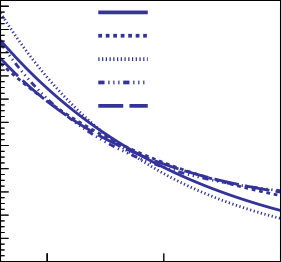
\includegraphics[width=0.9\textwidth]{BsDsK_TD/Combinatorial_Templates/BsDsK_BsMass}};
            \begin{scope}[x={(image.south east)},y={(image.north west)}]
                \node at (0.168, -0.025) {\num{6000}};
                \node at (0.582, -0.025) {\num{6500}};
                \node at (1.   , -0.025) {\num{7000}};
                \node[anchor=east] at (0.005, 0.) {\num{0}};
                \foreach \y in {2, 4, ..., 22}
                {
                    \tikzmath{\ypos = \y / 22.6; \ytext = \y / 1000;}
                    \node[anchor=east] at (0.005, \ypos) {\pgfmathprintnumber[fixed,precision=3,fixed zerofill=true]{\ytext}};
                }
                % Legend
                {
                    \fontsize{5.5}{6.6}\selectfont
                    \node[anchor=base west] at (0.523, 0.940) {\DsmNonRes};
                    \node[anchor=base west] at (0.523, 0.940 - 1 * 0.0888) {\DsmPhiPi};
                    \node[anchor=base west] at (0.523, 0.940 - 2 * 0.0888) {\DsmKstK};
                    \node[anchor=base west] at (0.523, 0.940 - 3 * 0.0888) {\DsmKPiPi};
                    \node[anchor=base west] at (0.523, 0.940 - 4 * 0.0888) {\DsmPiPiPi};
                }
                \node[anchor=east] at (1.0, -0.09) {\({m(\DsmpKpm)}~[\si{\MeVcc}]\)};
                \node[rotate=90,anchor=east,inner xsep=0pt,outer xsep=0pt] at (-0.16, 1.0) {PDF};
                \node[anchor=west] at (0.11, 0.92) {\large\lhcb};
            \end{scope}
        \end{tikzpicture}
        \caption{\Bs~mass.}
    \end{subfigure} \hfill%
    \begin{subfigure}{.48\textwidth} \centerfloat
        \begin{tikzpicture}
            \node[anchor=south west,inner sep=0] (image) at (0,0) {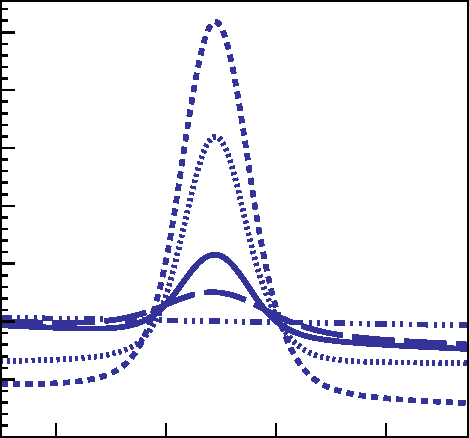
\includegraphics[width=0.9\textwidth]{BsDsK_TD/Combinatorial_Templates/BsDsK_DsMass}};
            \begin{scope}[x={(image.south east)},y={(image.north west)}]
                \foreach \x/\xtext in {1940, 1960, ..., 2000}
                {
                    \tikzmath{\xpos = (\x - 1940) / (2000 - 1940) * (0.822 - 0.12) + 0.12;}
                    \node at (\xpos, -0.025) {\(\xtext\)};
                }
                \node[anchor=east] at (0.005, 0.) {\num{0}};
                \foreach \y in {1, ..., 7}
                {
                    \tikzmath{\ypos = \y / 7.55; \ytext = \y / 200;}
                    \node[anchor=east] at (0.005, \ypos) {\pgfmathprintnumber[fixed,precision=3,fixed zerofill=true]{\ytext}};
                }
                \node[anchor=east] at (1.0, -0.09) {\({m(\Dsmp)}~[\si{\MeVcc}]\)};
                \node[rotate=90,anchor=east,inner xsep=0pt,outer xsep=0pt] at (-0.16, 1.0) {PDF};
                \node[anchor=east] at (0.91, 0.92) {\large\lhcb};
            \end{scope}
        \end{tikzpicture}
        \caption{\Dsmp~mass.}
    \end{subfigure} \par\bigskip
    \begin{subfigure}{.48\textwidth} \centerfloat
        \begin{tikzpicture}
            \node[anchor=south west,inner sep=0] (image) at (0,0) {\includegraphics[width=0.9\textwidth]{BsDsK_TD/Combinatorial_Templates/BsDsPi_CompDLLkpi}};
            \begin{scope}[x={(image.south east)},y={(image.north west)}]
                \foreach \x/\xtext in {0, ..., 2}
                {
                    \tikzmath{\xpos = (\x / 5) * 0.835 + 0.080; \xtext = (\x - 3) * 2;}
                    \node at (\xpos, -0.025) {\pgfmathprintnumber[fixed,precision=0,fixed zerofill=true]{\xtext}};
                }
                \foreach \x/\xtext in {3, ..., 5}
                {
                    \tikzmath{\xpos = (\x / 5) * 0.832 + 0.083; \xtext = (\x - 3) * 2;}
                    \node at (\xpos, -0.025) {\pgfmathprintnumber[fixed,precision=0,fixed zerofill=true]{\xtext}};
                }
                \node[anchor=east] at (0.005, 0.) {\num{0}};
                \foreach \y in {1, ..., 10}
                {
                    \tikzmath{\ypos = \y / 10.95; \ytext = \y / 200;}
                    \node[anchor=east] at (0.005, \ypos) {\pgfmathprintnumber[fixed,precision=3,fixed zerofill=true]{\ytext}};
                }
                % Legend
                {
                    \node[anchor=base west] at (0.167, 0.820) {\DsmNonRes};
                    \node[anchor=base west] at (0.167, 0.820 - 1 * 0.079) {\DsmPhiPi};
                    \node[anchor=base west] at (0.167, 0.820 - 2 * 0.079) {\DsmKstK};
                    \node[anchor=base west] at (0.167, 0.820 - 3 * 0.079) {\DsmKPiPi};
                    \node[anchor=base west] at (0.167, 0.820 - 4 * 0.079) {\DsmPiPiPi};
                }
                \node[anchor=east] at (1.0, -0.09) {\({\log(-\dllkpi)}\)};
                \node[rotate=90,anchor=east,inner xsep=0pt,outer xsep=0pt] at (-0.16, 1.0) {PDF};
                \node[anchor=west] at (0.11, 0.92) {\large\lhcb};
            \end{scope}
        \end{tikzpicture}
        \caption{Companion~\dllkpi for pions.}
    \end{subfigure} \hfill%
    \begin{subfigure}{.48\textwidth} \centerfloat
        \begin{tikzpicture}
            \node[anchor=south west,inner sep=0] (image) at (0,0) {\includegraphics[width=0.9\textwidth]{BsDsK_TD/Combinatorial_Templates/BsDsK_CompDLLkpi}};
            \begin{scope}[x={(image.south east)},y={(image.north west)}]
                \foreach \x/\xtext in {0, ..., 6}
                {
                    \tikzmath{\xpos = (\x / 6) * 0.883 + 0.117; \xtext = (\x + 4) * 0.5;}
                    \node at (\xpos, -0.025) {\pgfmathprintnumber[fixed,precision=1,fixed zerofill=true]{\xtext}};
                }
                \node[anchor=east] at (0.005, 0.) {\num{0}};
                \foreach \y in {1, ..., 10}
                {
                    \tikzmath{\ypos = \y / 10.44; \ytext = \y / 500;}
                    \node[anchor=east] at (0.005, \ypos) {\pgfmathprintnumber[fixed,precision=3,fixed zerofill=true]{\ytext}};
                }
                \node[anchor=east] at (1.0, -0.09) {\({\log(\dllkpi)}\)};
                \node[rotate=90,anchor=east,inner xsep=0pt,outer xsep=0pt] at (-0.16, 1.0) {PDF};
                \node[anchor=east] at (0.91, 0.92) {\large\lhcb};
            \end{scope}
        \end{tikzpicture}
        \caption{Companion~\dllkpi for kaons.}
    \end{subfigure}
    \caption{
        Combinatorial PDF~shape parameterisations of the \Bs~(top left) and \Dsm~(top right) invariant masses obtained from the fit to \BsDsK~candidates in upper-sideband data.
        The \dllkpi~distributions for \BsDsPi~(bottom left) and \BsDsK~companion tracks (bottom right) are also shown.}
    \label{fig:BsDsK_TD_Comb_Shape_Results}
\end{figure}

\subsection{Fit results}

The results of the multivariate fit to the final state~\DsmPip are listed in \cref{tab:BsDsK_TD_DsPi_MDFit_Results}, and shown in \cref{fig:BsDsK_TD_DsPi_MDFit_Results}.
The total signal yield is \num{96942 +- 345}~candidates.

The fit results of the fit to \DspmKmp~candidates are listed in \cref{tab:BsDsK_TD_DsK_MDFit_Results}, and shown in \cref{fig:BsDsK_TD_DsK_MDFit_Results}.
The total signal yield is \num{5955 +- 90}~candidates.

\begin{landscape}
\begin{table}[p] \centerfloat
    \caption{
        Results of the multivariate fit to the final state~\DsmPip .
        The \(N\)~represent the yields of the signal, combinatorial, and backgrounds without fixed yields, and the \DCBmu~and \(R\)~parameters are the mean and mass resolution scale factor of the signal, respectively.
        The~\(s_{\text{comb}}\) are the slopes of combinatorial background, in units of~\num{e-3}.
        The fraction~\(f_{\text{comb, \Bs}}\) is the fraction between the exponential and constant components of the combinatorial parameterisation of the \Bs~invariant mass, whereas \(f_{\text{comb, \Dsm}}\)~represents the fraction between the combinatorial exponential and DCB~shapes in the \Dsm~mass.
        \(f_{\text{comb, \dll}}\)~is the fraction between the pion and kaon components in the \dllkpi~combinatorial shape.
        Finally, \(f_{\text{\BsDsstPi}}\)~is the fraction between the partially reconstructed background \BsDsstPi~and the decay~\BdDsPi.}
    \label{tab:BsDsK_TD_DsPi_MDFit_Results}
    \begin{tabular}{lccccc}
        \toprule
        Parameter & \DspmNonRes  & \DspmPhiPi & \DspmKstK & \DspmKPiPi & \DspmPiPiPi \tabularnewline
        \midrule
        \(N_{\BsDsPi}\)            & \err{16\,056}{145}   & \err{34\,355}{201}   & \err{25\,596}{173}   & \err{5728}{86}      & \err{15\,206}{145} \tabularnewline
        \midrule
        \(N_{\text{backgrounds}}\) & \err{\0\,\0\087}{\025} & \err{\0\,\0215}{\031} & \err{\0\,\0168}{\031} & \err{\0\038}{14} & \err{\0\,\0\094}{\024} \tabularnewline[.3ex]
        \rowcolor{tableshade}
        \(N_{\text{comb}}\)        & \err{\0\,9185}{123} & \err{\0\,3116}{103} & \err{\0\,3769}{\093} & \err{2765}{65} & \err{\0\,6952}{109} \tabularnewline[.3ex]
        \midrule
        \(\DCBmu_{\Bs}\)~(\si{\MeVcc})   & \multicolumn{5}{c}{\raisebox{.5ex}{\rule{.33\linewidth}{.3pt}}~\err{5365.10}{0.06}~\raisebox{.5ex}{\rule{.33\linewidth}{.3pt}}} \tabularnewline[.3ex]
        \rowcolor{tableshade}
        \(\RBs\)                   & \err{1.082}{0.010} & \err{1.082}{0.006} & \err{1.082}{0.007} & \err{1.077}{0.016} & \err{1.070}{0.010} \tabularnewline[.3ex]
        \(\DCBmu_{\Dsm}\)~(\si{\MeVcc}) & \multicolumn{5}{c}{\raisebox{.5ex}{\rule{.33\linewidth}{.3pt}}~\err{1969.80}{0.02}~\raisebox{.5ex}{\rule{.33\linewidth}{.3pt}}} \tabularnewline[.3ex]
        \rowcolor{tableshade}
        \(\RDs\)                   & \err{1.040}{0.009} & \err{1.056}{0.006} & \err{1.053}{0.006} & \err{1.047}{0.015} & \err{1.049}{0.010} \tabularnewline[.3ex]
        \midrule
        \(s_{\text{comb, \Bs}} \times \num{e3}\) & \err{-7.35}{0.28} & \err{-9.74}{0.60} & \err{-9.22}{0.53} & \err{-6.28}{0.99} & \err{-4.70}{0.53} \tabularnewline[.3ex]
        \rowcolor{tableshade}
        \(f_{\text{comb, \Bs}}\)   & \err{\n0.86}{0.02} & \err{\n0.75}{0.03} & \err{\n0.75}{0.03} & \err{\n0.52}{0.06} & \err{\n0.70}{0.06} \tabularnewline[.3ex]
        \(s_{\text{comb, \Dsm}} \times \num{e3}\) & \err{-0.29}{0.46} & \err{-4.66}{0.99} & \err{-4.14}{0.78} & \err{-1.23}{0.84} & \err{-4.13}{0.53} \tabularnewline[.3ex]
        \rowcolor{tableshade}
        \(f_{\text{comb, \Dsm}}\)  & \err{\n0.98}{0.01} & \err{\n0.73}{0.02} & \err{\n0.89}{0.02} & \err{\n0.95}{0.02} & \err{\n0.97}{0.02} \tabularnewline[.3ex]
        \(f_{\text{comb, \dll}}\)  & \err{\n0.86}{0.01} & \err{\n0.76}{0.02} & \err{\n0.81}{0.02} & \err{\n1.00}{0.01} & \err{\n1.00}{0.01} \tabularnewline
        \midrule
        \(f_{\text{\BsDsstPi}}\)   & \multicolumn{5}{c}{\raisebox{.5ex}{\rule{.35\linewidth}{.3pt}}~\erra{0.00}{0.08}{0.00}~\raisebox{.5ex}{\rule{.35\linewidth}{.3pt}}} \tabularnewline
        \bottomrule
     \end{tabular}
\end{table}
\end{landscape}

\begin{figure}[hp] \centerfloat
    \begin{subfigure}{\textwidth} \centerfloat
        \begin{tikzpicture}
            \node[anchor=south west,inner sep=0] (image) at (0,0) {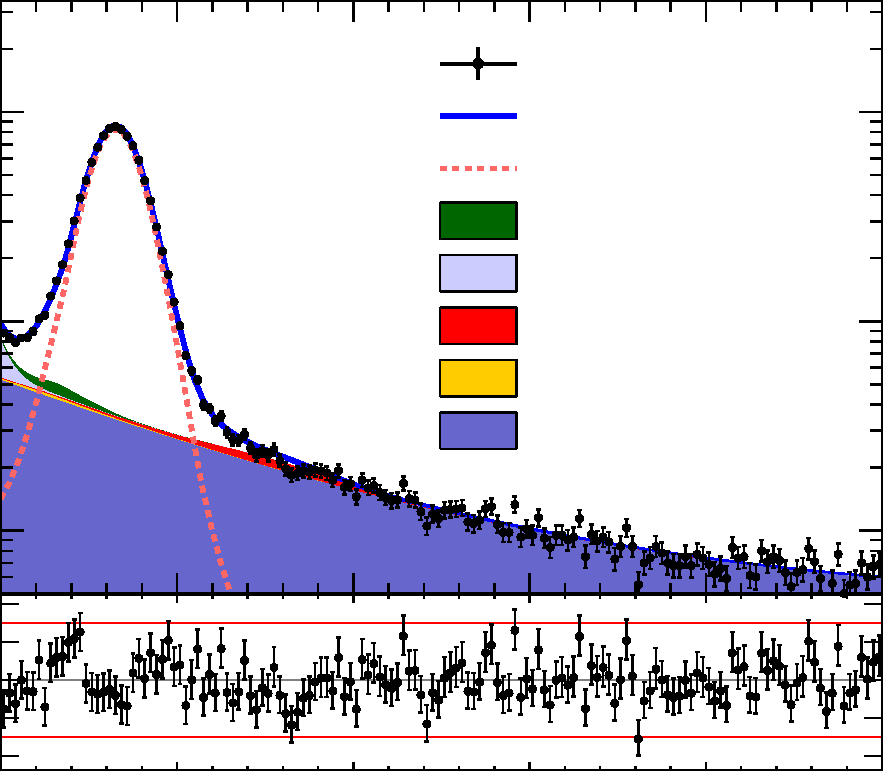
\includegraphics[width=0.9\textwidth]{BsDsK_TD/MDFit_Results/mass_Bs2DsPi_BeautyMass_both_all_run1_nominal}};
            \begin{scope}[x={(image.south east)},y={(image.north west)}]
                \foreach \x/\xtext in {5300, 5400, ..., 5800}
                {
                    \tikzmath{\xpos = (\x - 5300) / (5800 - 5300);}
                    \node at (\xpos, -0.025) {\(\xtext\)};
                }
                \node[anchor=base east] at (0.005, 0.297       ) {\(10^{2}\)};
                \node[anchor=base east] at (0.005, 0.297+1*.272) {\(10^{3}\)};
                \node[anchor=base east] at (0.005, 0.297+2*.272) {\(10^{4}\)};
                \foreach \p in {0, ..., 4}
                {
                    \tikzmath{\ypos = (\p / 4) * 0.198 + .020; \ptext = (\p - 2) * 2;}
                    \node[anchor=east] at (0.005, \ypos) {\(\scriptstyle\pgfmathprintnumber[fixed,precision=0,fixed zerofill=true]{\ptext}\)};
                }
                \node[anchor=east] at (1.0, -0.09) {\({m(\DsmpPipm)}~[\si{\MeVcc}]\)};
                \node[rotate=90,anchor=east,inner xsep=0pt,outer xsep=0pt] at (-0.11, 1.0) {\({\text{Candidates}/(\SI{5.0}{\MeVcc})}\)};
                \node[anchor=west] at (0.06, 0.92) {\Huge\lhcb};
                % Legend
                {
                    \node[anchor=base west] at (0.585, 0.906) {Data};
                    \node[anchor=base west] at (0.585, 0.906 - 1 * 0.0682) {Total fit};
                    \node[anchor=base west] at (0.585, 0.906 - 2 * 0.0682) {\BsDsPi~signal};
                    \node[anchor=base west] at (0.585, 0.906 - 3 * 0.0682) {\BsDsK};
                    \node[anchor=base west] at (0.585, 0.906 - 4 * 0.0682) {\decay{\BorBsz}{\DsorDssm\pip}};
                    \node[anchor=base west] at (0.585, 0.906 - 5 * 0.0682) {\LbLcPi};
                    \node[anchor=base west] at (0.585, 0.906 - 6 * 0.0682) {\BdDPi};
                    \node[anchor=base west] at (0.585, 0.906 - 7 * 0.0682) {Combinatorial};
                }
            \end{scope}
        \end{tikzpicture}
        \caption{\DsmpPipm~invariant mass.}
    \end{subfigure} \par\bigskip
    \begin{subfigure}{.48\textwidth} \centerfloat
        \begin{tikzpicture}
            \node[anchor=south west,inner sep=0] (image) at (0,0) {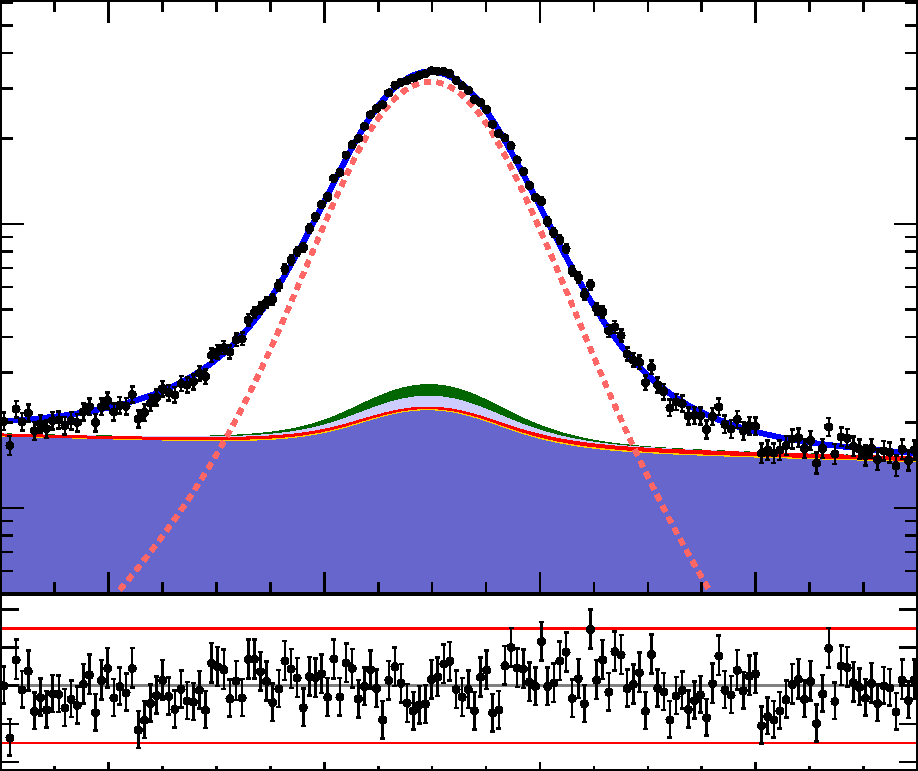
\includegraphics[width=0.9\textwidth]{BsDsK_TD/MDFit_Results/mass_Bs2DsPi_CharmMass_both_all_run1_nominal}};
            \begin{scope}[x={(image.south east)},y={(image.north west)}]
                \fontsize{8}{9.6}\selectfont
                \foreach \x/\xtext in {1940, 1960, ..., 2000}
                {
                    \tikzmath{\xpos = (\x - 1940) / (2000 - 1940) * (0.822 - 0.12) + 0.12;}
                    \node at (\xpos, -0.032) {\(\xtext\)};
                }
                \node[anchor=base east] at (0.005, 0.327) {\(10^{2}\)};
                \node[anchor=base east] at (0.005, 0.694) {\(10^{3}\)};
                \foreach \p in {0, ..., 4}
                {
                    \tikzmath{\ypos = (\p / 4) * 0.198 + .013; \ptext = (\p - 2) * 2;}
                    \node[anchor=east] at (0.005, \ypos) {\(\scriptstyle\pgfmathprintnumber[fixed,precision=0,fixed zerofill=true]{\ptext}\)};
                }
                \node[anchor=east] at (1.0, -0.11) {\({m(\Dsmp)}~[\si{\MeVcc}]\)};
                \node[rotate=90,anchor=east,inner xsep=0pt,outer xsep=0pt] at (-0.13, 1.0) {\({\text{Candidates}/(\SI{0.85}{\MeVcc})}\)};
                \node[anchor=west] at (0.06, 0.92) {\Large\lhcb};
            \end{scope}
        \end{tikzpicture}
        \caption{\Dsmp~invariant mass.}
    \end{subfigure} \hfill%
    \begin{subfigure}{.48\textwidth} \centerfloat
        \begin{tikzpicture}
            \node[anchor=south west,inner sep=0] (image) at (0,0) {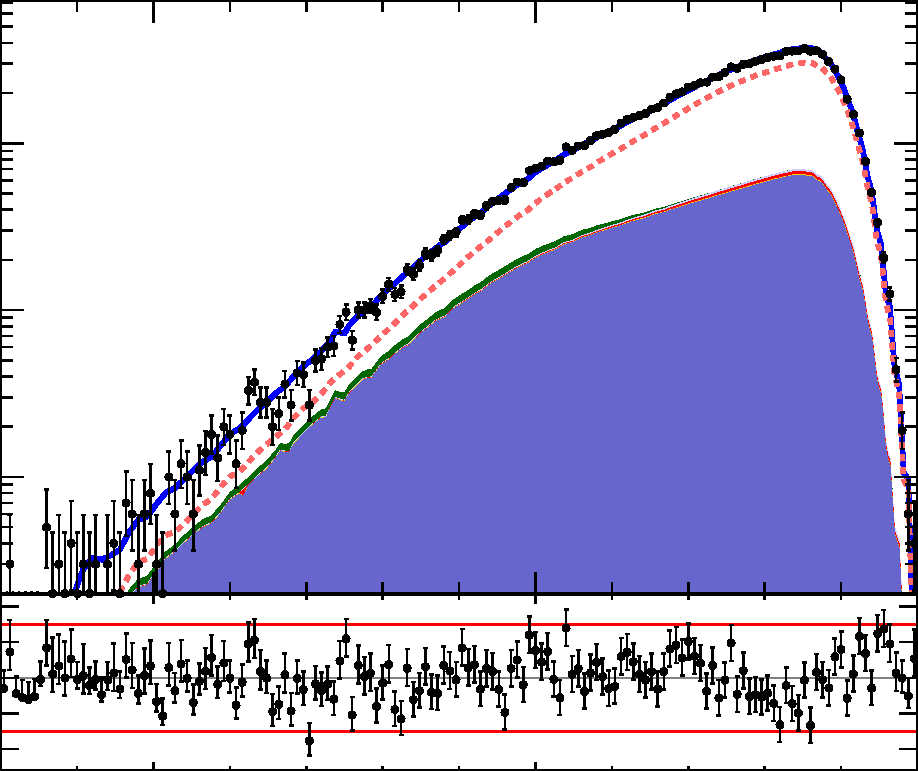
\includegraphics[width=0.9\textwidth]{BsDsK_TD/MDFit_Results/mass_Bs2DsPi_BacPIDK_both_all_run1_nominal}};
            \begin{scope}[x={(image.south east)},y={(image.north west)}]
                \fontsize{8}{9.6}\selectfont
                \node at (0.163, -0.032) {\num{-5}};
                \node at (0.583, -0.032) {\num{ 0}};
                \node at (1.   , -0.032) {\num{ 5}};
                \node[anchor=base east] at (0.005, 0.362       ) {\(10\)};
                \node[anchor=base east] at (0.005, 0.362+1*.217) {\(10^{2}\)};
                \node[anchor=base east] at (0.005, 0.362+2*.217) {\(10^{3}\)};
                \foreach \p in {0, ..., 4}
                {
                    \tikzmath{\ypos = (\p / 4) * 0.198 + .013; \ptext = (\p - 2) * 2;}
                    \node[anchor=east] at (0.005, \ypos) {\(\scriptstyle\pgfmathprintnumber[fixed,precision=0,fixed zerofill=true]{\ptext}\)};
                }
                \node[anchor=east] at (1.0, -0.09) {\({\log(-\dllkpi)}\)};
                \node[rotate=90,anchor=east,inner xsep=0pt,outer xsep=0pt] at (-0.13, 1.0) {\({\text{Candidates}/0.12}\)};
                \node[anchor=west] at (0.06, 0.92) {\large\lhcb};
            \end{scope}
        \end{tikzpicture}
        \caption{Companion~\dllkpi.}
    \end{subfigure}
    \caption{
        Results of the multivariate fit to \BsDsPi~candidates.}
    \label{fig:BsDsK_TD_DsPi_MDFit_Results}
\end{figure}

\begin{landscape}
\begin{table}[p] \centerfloat
    \caption{
        Results of the multivariate fit to the final state~\DsmpKpm.
        The \(N\)~represent yields, and the \DCBmu~are the mean values of the \Bs~and \Dsmp~signal shapes.
        The \(s_{\text{comb}}\)~are the slopes of combinatorial background, in units of~\num{e-3}.
        The fraction~\(f_{\text{comb, \Bs}}\) is the fraction between the exponential and constant components in the \DsmpKpm~mass, whereas \(f_{\text{comb, \Dsmp}}\)~represents the fraction between the combinatorial exponential and DCB~shapes in the \Dsmp~mass.
        The \(f_{\text{comb, \dll}}\)~are the fractions between the components in the \dllkpi~combinatorial shape: \(f_{\text{comb, \dll,1}}\)~is the fraction of pions and \({(1 - f_{\text{comb, \dll,1}}) f_{\text{comb, \dll,2}}}\)~corresponds to the fraction of kaons.
        Finally, \(f_{\BsDsPi}\)~is the fraction between \BsDsPi~and the partially reconstructed backgrounds, and \(f_{\Lb}\)~is the fraction between all backgrounds of the form~\BsDsOrDsstPi and the sum of the two backgrounds~\LbDsOrDsstp.}
    \label{tab:BsDsK_TD_DsK_MDFit_Results}
    \begin{tabular}{lccccc}
        \toprule
        Parameter & \DsmNonRes & \DsmPhiPi & \DsmKstK & \DsmKPiPi & \DsmPiPiPi \tabularnewline
        \midrule
        \(N_{\BsDsK}\)              & \err{1055}{38}   & \err{1957}{51}   & \err{1616}{46}   & \err{\0391}{24}      & \err{\0936}{37} \tabularnewline
        \midrule
        \(N_{\BdDsK}\)              & \err{\0\032}{10} & \err{\0\049}{13} & \err{\0\050}{12} & \err{\0\024}{\07} & \err{\0\041}{11} \tabularnewline[.3ex]
        \rowcolor{tableshade}
        \(N_{\text{backgrounds}}\)  & \err{\0676}{36} & \err{1513}{57} & \err{1062}{50} & \err{\0208}{23} & \err{\0763}{43} \tabularnewline[.3ex]
        \(N_{\text{comb}}\)         & \err{1370}{47} & \err{\0736}{55} & \err{\0707}{53} & \err{1113}{40} & \err{2173}{59} \tabularnewline[.3ex]
        \midrule
        \(\DCBmu_{\Bs}\)~(\si{\MeVcc})   & \multicolumn{5}{c}{\raisebox{.5ex}{\rule{.33\linewidth}{.3pt}}~\err{5365.2}{0.2}~\raisebox{.5ex}{\rule{.33\linewidth}{.3pt}}} \tabularnewline[.3ex]
        \rowcolor{tableshade}
        \(\DCBmu_{\Dsmp}\)~(\si{\MeVcc}) & \multicolumn{5}{c}{\raisebox{.5ex}{\rule{.33\linewidth}{.3pt}}~\err{1969.7}{0.1}~\raisebox{.5ex}{\rule{.33\linewidth}{.3pt}}} \tabularnewline[.3ex]
        \midrule
        \(s_{\text{comb, \Bs}} \times \num{e3}\)   & \err{-6.8\0}{1.0\0} & \err{-12.2}{0.9\0}  & \err{-7.9\0}{1.5\0} & \err{-1.40}{0.24}   & \err{-1.63}{0.18} \tabularnewline[.3ex]
        \rowcolor{tableshade}
        \(f_{\text{comb, \Bs}}\)    & \err{\n0.64}{0.07} & \err{\n0.37}{0.05} & \err{\n0.63}{0.08} & -- & -- \tabularnewline[.3ex]
        \(s_{\text{comb, \Dsmp}} \times \num{e3}\) & \err{-0.4\0}{0.1\0} & \err{-7.6\0}{2.1\0} & \err{-1.6\0}{1.9\0} & \err{-1.0\0}{1.2\0} & \err{-3.8\0}{0.9\0} \tabularnewline[.3ex]
        \rowcolor{tableshade}
        \(f_{\text{comb, \Dsmp}}\)  & \err{\n0.99}{0.09} & \err{\n0.61}{0.05} & \err{\n0.72}{0.05} & \err{\n1.00}{0.07} & \err{\n1.00}{0.02} \tabularnewline[.3ex]
        \(f_{\text{comb, \dll,1}}\) & \err{\n0.28}{0.04} & \err{\n0.12}{0.07} & \err{\n0.31}{0.07} & \err{\n0.01}{0.04} & \err{\n0.15}{0.03} \tabularnewline
        \rowcolor{tableshade}
        \(f_{\text{comb, \dll,2}}\) & \err{\n0.77}{0.08} & \err{\n0.55}{0.09} & \err{\n0.93}{0.16} & \err{\n0.66}{0.07} & \err{\n0.60}{0.05} \tabularnewline
        \midrule
        \(f_{\BsDsPi}\)             & \multicolumn{5}{c}{\raisebox{.5ex}{\rule{.33\linewidth}{.3pt}}~\err{0.729}{0.021}~\raisebox{.5ex}{\rule{.33\linewidth}{.3pt}}} \tabularnewline
        \rowcolor{tableshade}
        \(f_{\Lb}\)                 & \multicolumn{5}{c}{\raisebox{.5ex}{\rule{.33\linewidth}{.3pt}}~\err{0.923}{0.023}~\raisebox{.5ex}{\rule{.33\linewidth}{.3pt}}} \tabularnewline
        \bottomrule
     \end{tabular}
\end{table}
\end{landscape}

\begin{figure}[hp] \centerfloat
    \begin{subfigure}{\textwidth} \centerfloat
        \begin{tikzpicture}
            \node[anchor=south west,inner sep=0] (image) at (0,0) {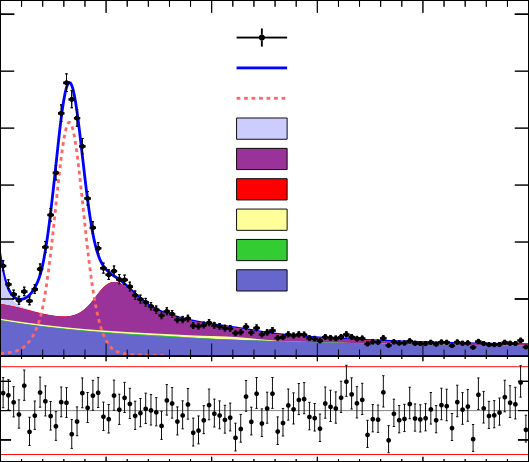
\includegraphics[width=0.9\textwidth]{BsDsK_TD/MDFit_Results/mass_Bs2DsK_BeautyMass_both_all_run1_nominal}};
            \begin{scope}[x={(image.south east)},y={(image.north west)}]
                \foreach \x/\xtext in {5300, 5400, ..., 5800}
                {
                    \tikzmath{\xpos = (\x - 5300) / (5800 - 5300);}
                    \node at (\xpos, -0.025) {\(\xtext\)};
                }
                \foreach \y in {0, ..., 6}
                {
                    \tikzmath{\ypos = (\y / 6) * 0.740 + 0.217; \ytext = 200 * \y;}
                    \node[anchor=base east] at (0.005, \ypos) {\(\pgfmathprintnumber[fixed,precision=0,fixed zerofill=true,1000 sep={}]{\ytext}\)};
                }
                \foreach \p in {0, ..., 2}
                {
                    \tikzmath{\ypos = (\p / 2) * 0.127 + .048; \ptext = (\p - 1) * 2;}
                    \node[anchor=east] at (0.005, \ypos) {\(\scriptstyle\pgfmathprintnumber[fixed,precision=0,fixed zerofill=true]{\ptext}\)};
                }
                \node[anchor=east] at (1.0, -0.09) {\({m(\DsmpKpm)}~[\si{\MeVcc}]\)};
                \node[rotate=90,anchor=east,inner xsep=0pt,outer xsep=0pt] at (-0.11, 1.0) {\({\text{Candidates}/(\SI{5.0}{\MeVcc})}\)};
                \node[anchor=west] at (0.06, 0.92) {\Huge\lhcb};
                % Legend
                {
                    \node[anchor=base west] at (0.55, 0.906) {Data};
                    \node[anchor=base west] at (0.55, 0.906 - 1 * 0.0656) {Total fit};
                    \node[anchor=base west] at (0.55, 0.906 - 2 * 0.0656) {\BsDsK~signal};
                    \node[anchor=base west] at (0.55, 0.906 - 3 * 0.0656) {\decay{\BorBsz}{\DsorDssmp\KorKstpm}};
                    \node[anchor=base west] at (0.55, 0.906 - 4 * 0.0656) {\decay{\Bs}{\DsorDssm(\pip, \rhop)}};
                    \node[anchor=base west] at (0.55, 0.906 - 5 * 0.0656) {\decay{\Bd}{\Dm(\pip, \Kp)}};
                    \node[anchor=base west] at (0.55, 0.906 - 6 * 0.0656) {\LbDsOrDsstp};
                    \node[anchor=base west] at (0.55, 0.906 - 7 * 0.0656) {\decay{\Lb}{\Lcp(\pim, \Km)}};
                    \node[anchor=base west] at (0.55, 0.906 - 8 * 0.0656) {Combinatorial};
                }
            \end{scope}
        \end{tikzpicture}
        \caption{\DsmpKpm~invariant mass.}
    \end{subfigure} \par\bigskip
    \begin{subfigure}{.48\textwidth} \centerfloat
        \begin{tikzpicture}
            \node[anchor=south west,inner sep=0] (image) at (0,0) {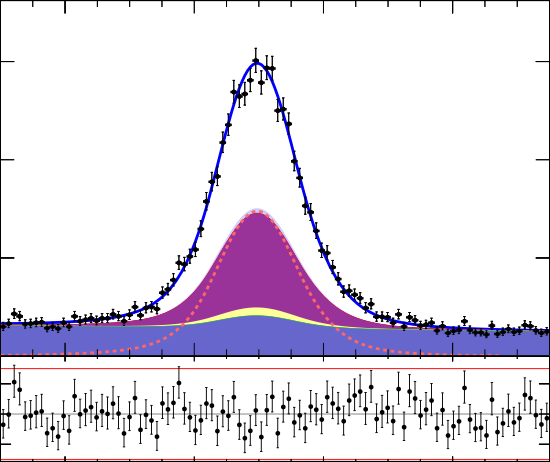
\includegraphics[width=0.9\textwidth]{BsDsK_TD/MDFit_Results/mass_Bs2DsK_CharmMass_both_all_run1_nominal}};
            \begin{scope}[x={(image.south east)},y={(image.north west)}]
                \fontsize{8}{9.6}\selectfont
                \foreach \x/\xtext in {1940, 1960, ..., 2000}
                {
                    \tikzmath{\xpos = (\x - 1940) / (2000 - 1940) * (0.822 - 0.12) + 0.12;}
                    \node at (\xpos, -0.032) {\(\xtext\)};
                }
                \foreach \y in {0, ..., 3}
                {
                    \tikzmath{\ypos = (\y / 3) * 0.640 + 0.21; \ytext = 200 * \y;}
                    \node[anchor=base east] at (0.005, \ypos) {\(\pgfmathprintnumber[fixed,precision=0,fixed zerofill=true]{\ytext}\)};
                }
                \foreach \p in {0, ..., 2}
                {
                    \tikzmath{\ypos = (\p / 2) * 0.127 + .044; \ptext = (\p - 1) * 2;}
                    \node[anchor=east] at (0.005, \ypos) {\(\scriptstyle\pgfmathprintnumber[fixed,precision=0,fixed zerofill=true]{\ptext}\)};
                }
                \node[anchor=east] at (1.0, -0.11) {\({m(\Dsmp)}~[\si{\MeVcc}]\)};
                \node[rotate=90,anchor=east,inner xsep=0pt,outer xsep=0pt] at (-0.13, 1.0) {\({\text{Candidates}/(\SI{0.85}{\MeVcc})}\)};
                \node[anchor=west] at (0.06, 0.92) {\Large\lhcb};
            \end{scope}
        \end{tikzpicture}
        \caption{\Dsmp~invariant mass.}
    \end{subfigure} \hfill%
    \begin{subfigure}{.48\textwidth} \centerfloat
        \begin{tikzpicture}
            \node[anchor=south west,inner sep=0] (image) at (0,0) {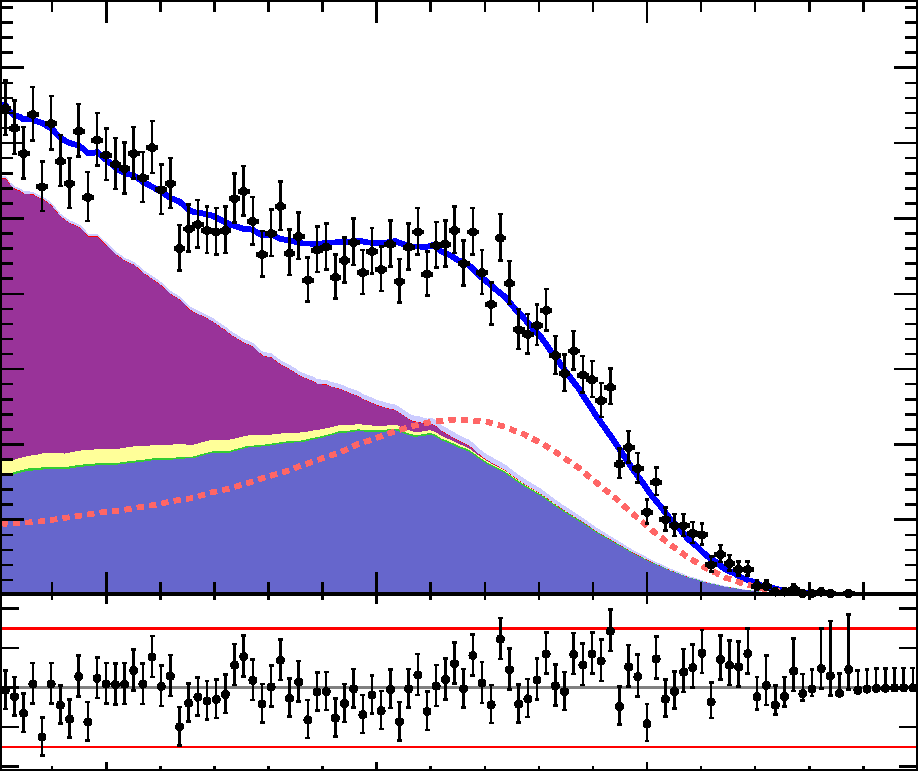
\includegraphics[width=0.9\textwidth]{BsDsK_TD/MDFit_Results/mass_Bs2DsK_BacPIDK_both_all_run1_nominal}};
            \begin{scope}[x={(image.south east)},y={(image.north west)}]
                \fontsize{8}{9.6}\selectfont
                \foreach \x/\xtext in {0, ..., 3}
                {
                    \tikzmath{\xpos = (\x / 3) * 0.883 + 0.117; \xtext = \x + 2;}
                    \node at (\xpos, -0.032) {\pgfmathprintnumber[fixed,precision=0,fixed zerofill=true]{\xtext}};
                }
                \foreach \y in {1, ..., 7}
                {
                    \tikzmath{\ypos = (\y / 7) * 0.682 + 0.210; \ytext = 50 * \y;}
                    \node[anchor=base east] at (0.005, \ypos) {\(\pgfmathprintnumber[fixed,precision=0,fixed zerofill=true]{\ytext}\)};
                }
                \foreach \p in {0, ..., 4}
                {
                    \tikzmath{\ypos = (\p / 4) * 0.205 + .007; \ptext = (\p - 2) * 2;}
                    \node[anchor=east] at (0.005, \ypos) {\(\scriptstyle\pgfmathprintnumber[fixed,precision=0,fixed zerofill=true]{\ptext}\)};
                }
                \node[anchor=east] at (1.0, -0.09) {\({\log(\dllkpi)}\)};
                \node[rotate=90,anchor=east,inner xsep=0pt,outer xsep=0pt] at (-0.13, 1.0) {\({\text{Candidates}/0.03}\)};
                \node[anchor=west] at (0.70, 0.92) {\large\lhcb};
            \end{scope}
        \end{tikzpicture}
        \caption{Companion~\dllkpi.}
    \end{subfigure}
    \caption{
        Results of the multivariate fit to \BsDsK~candidates.}
    \label{fig:BsDsK_TD_DsK_MDFit_Results}
\end{figure}

\clearpage
\subsection{Fit validation}
\label{sec:BsDsK_TD_MDFit_Validation}

The multivariate fit procedure is validated by applying it to several subsamples, repeating the entire procedure described in this \lcnamecref{sec:BsDsK_TD_MDFit_Validation}
The data is split by:
%
\begin{enumerate}
    \item \lhcb~magnet polarity;
    \item centre-of-mass energy;
    \item BDT~response;
    \item \Bs~momentum, split at~\SI{120}{\GeVc}.
\end{enumerate}
%
In the latter two cases, the split value is chosen such that the remaining samples have roughly the same signal yields in simulation.
To check the results of the splits, the sum of the signal yields of the split fits are compared with the signal yield of the fit on the full data set.
These yields are shown in \cref{tab:BsDsK_TD_MDFit_Split}.
The individual fits each have good quality, and the yields also show good agreement.
To further validate these splits, the decay-time fit is also performed separately on the partial data samples (see \cref{sec:BsDsK_TD_Syst}).
%
\begin{table}[htb] \centerfloat
    \caption{
        Total yields of the full and split data sample, resulting from the respective multivariate fits.}
    \label{tab:BsDsK_TD_MDFit_Split}
    \rowcolors{1}{tableshade}{}
    \begin{tabular}{lS[table-format=5(3)]S[table-format=4(2)]}
        \hiderowcolors \toprule
        \multirow{2}{*}[-2pt]{Sample} & \multicolumn{2}{c}{Total yield} \tabularnewline
        \cmidrule(lr){2-3}
                    & {\BsDsPi}    & {\BsDsK} \tabularnewline
        \showrowcolors \midrule
        Full sample & 96942 +- 345 & 5955 +- 90 \tabularnewline
        Split 1     & 96985 +- 345 & 5962 +- 91 \tabularnewline
        Split 2     & 97010 +- 345 & 5953 +- 90 \tabularnewline
        Split 3     & 96334 +- 342 & 5873 +- 90 \tabularnewline
        Split 4     & 97170 +- 346 & 5911 +- 95 \tabularnewline
        \bottomrule
    \end{tabular}
\end{table}

\clearpage

\setchapterpreamble{
    \lettrine{T}{his}~\lcnamecref{chp:BsDsK_TD} discusses the decay-time fit to the \BsDsK~sample obtained in \cref{chp:BsDsK_TD_Data}.
    This fit yields five \CP-violation parameters, \Cpar, \Spar, \Sbpar, \Dpar, and~\Dbpar, from which the CKM~parameter \CPgamma~is subsequently extracted.}
\chapter[\CP~violation in \BsDsK]{Time-dependent measurement of \CP~violation in~\BsDsK}
\label{chp:BsDsK_TD}

\vspace*{\fill}
\minitoc

\clearpage
\section{Decay-time resolution} \label{sec:BsDsK_TD_Res}

The oscillation period of the \Bs~system is of the same order of magnitude as the time resolution of the detector, which implies that the decay-time distribution of the \Bs~candidates is significantly diluted by the resolution.
This is accounted for in the decay-time fit, and in order to do so, the resolution is determined for each event.

The decay time~\(t\) is determined by a fit to the position of the \Bs~decay vertex~\(\vec{x}_\text{SV}\), its reconstructed momentum vector \(\vec{\ptot}\), and its proper decay time~\(t\), using the constraint
%
\begin{equation}
    \vec{x}_{\text{SV}} - \vec{x}_{\text{PV}} = t \dfrac{\vec{\ptot}}{m_{\Bs}} \rlap{,}
\end{equation}
%
where the position of the~PV~\(\vec{x}_{\text{PV}}\) is fixed by other tracks in the event and \(m_{\Bs}\)~is the known mass of the \Bs~meson~\cite{PDG}.
By excluding the four tracks from which the~SV is reconstructed from the PV~reconstruction, the correlation between~\(\vec{x}_{\text{PV}}\) and the other variables is nullified.

Input to this fit are the reconstructed tracks of the four decay particles~(\({\decay{\Bs}{\Dsmp(\to\KmpKPi)\Kpm}}\)) and their covariances resulting from the known detector resolution, multiple scattering, and kinematics.
As a result, both the decay time~\(t\) and the error on the decay time~\(\dt\) can be determined.
This error is called the per-event decay-time error throughout this \lcnamecref{sec:BsDsK_TD_Res}.
The error on the PV~location is negligible compared to that on the SV~location, and the correlation between \(\vec{x}_{\text{PV}}\)~and \(\vec{\ptot}\)~is small because of the way these variables are determined from track fits.
Consequently, \(\dt\)~is dominated by the errors on the SV~reconstruction and momentum determination, which in turn are dominated by the hit resolution in the tracking stations and the amount of detector material traversed.

\subsection{Decay-time error calibration} \label{sec:BsDsK_TD_Res_Calib}
The reconstructed per-event decay-time error provides a measure for the underlying resolution.
However, it is found that the per-event decay-time error somewhat underestimates the actual decay-time resolution, and thus must be calibrated before it can be used as input to the fit.
This calibration is done by using a sample of prompt \Dspm~candidates (\DspmKKPi) from data, and combining each candidate with a random track (again labelled as companion track) also originating from the~PV (see \cref{fig:BsDsK_TD_Res_Topology}).
The combination of these four tracks has kinematics similar to those of the signal process, except that the true decay time of each of these events is now known to be~\num{0}.
By reconstructing the decay time and taking the difference with~\num{0}, the resolution is obtained.
To reject possible contributions from real \Bs~mesons in this calibration procedure, the resolution is determined from events with a negative reconstructed decay time.
The decay-time resolution is determined for the final state~\DspmKKPi.
The difference in decay-time resolution for the other modes is smaller than~\SI{2}{\percent} as obtained from simulation, and is ignored.

\begin{figure}[htb] \centerfloat
    \begin{tikzpicture}[font=\captionfont]
        \coordinate (PV) at (0, 0);
        \coordinate (p1) at (-3, 0);
        \coordinate (p2) at (3, 0);
        \coordinate (comp) at (4, -2);
        \coordinate (h1) at (1.5, 1.25);
        \coordinate (h2) at (1.5, 1);
        \coordinate (h3) at (1.5, 0.75);

        \draw [thick,->] (p1) -- (PV) node [at start,anchor=north west] {\normalsize \proton} node [at end,anchor=north] {PV};
        \draw [thick,->] (p2) -- (PV) node [at start,anchor=north east] {\normalsize \proton};
        \draw (PV) -- (comp) node [midway,above=-0.075,sloped] {companion track};
        \draw (PV) -- (h1) node [midway,above,sloped] {\Dspm};
        \draw (PV) -- (h2) node {};
        \draw (PV) -- (h3) node {};

        \draw [dashed] (PV) -- (-1.2,  2);
        \draw [dashed] (PV) -- ( 2.3, -2);
        \draw [dashed] (PV) -- ( 3,    0.4);
        \draw [dashed] (PV) -- (-3,    0.9) node [midway,above,sloped] {other tracks};
        \draw [dashed] (PV) -- (-3,   -1.5);
    \end{tikzpicture}
    \caption{
        Decay topology of prompt \Dspm~candidates combined with a random track, which are used to calibrate the decay-time resolution.}
    \label{fig:BsDsK_TD_Res_Topology}
\end{figure}

The prompt \Dspm~sample and companion tracks are selected according to the same procedure as specified in \cref{sec:stripping}, except that some constraints are relaxed.
The companion track is not required to have a minimal~\chisqip, and the combination of \Dspm~candidate and companion track is not required to have a minimal displacement from the~PV, or to point back at it.
Loosening these requirements is necessary to produce a decay-time unbiased sample.
Some additional constraints are applied: the number of reconstructed~PVs is required to be~\num{1}, the flight-distance~\chisq of the \Dspm~combination with respect to the~PV is required to be~\({< \num{2}}\), and the companion track \dllmupi~to be \({< \num{2}}\).

To obtain a signal sample, combinatorial \Dspm~combinations are statistically subtracted from the sample using the \sfit~method~\cite{Yuehong_sFit}, by performing a fit to the \KKPi~invariant mass.
The \Dspm~component of this fit is defined as a double Crystal~Ball~(DCB) shape with common mean~\DCBmu and width~\DCBs, and the combinatorial background is parameterised as an exponential.
The results of the fit are shown in \cref{tab:BsDsK_TD_Res_sFit_Results,fig:BsDsK_TD_Res_sFit_Results}.
%
\begin{table}[htb] \centerfloat
    \caption{
        Result of the fit to the \KKPi~invariant mass of the prompt sample.
        Values quoted without an error are fixed in the fit.}
    \label{tab:BsDsK_TD_Res_sFit_Results}
    \rowcolors{2}{tableshade}{}
    \sisetup{table-number-alignment=right}
    \begin{tabular}{lS[table-format=6.3(3)]}
        \toprule
        Parameter & {Fitted value}\tabularnewline
        \midrule
        \(N_{\text{prompt~\Dspm}}\)  & 101882     +- 1635 \tabularnewline
        \(N_{\text{combinatorial}}\) & 563671     +- 2677 \tabularnewline
        \DCBmu~(\si{\MeVcc})         &   1969.80  +-    0.01  \tabularnewline
        \DCBs~(\si{\MeVcc})          &      6.220 +-    0.012 \tabularnewline
        \midrule
        \DCBaL & -1.24 \tabularnewline
        \DCBaR &  1.34 \tabularnewline
        \DCBnL &  6.67 \tabularnewline
        \DCBnR &  3.43 \tabularnewline
        \DCBf  &  0.5  \tabularnewline
        \bottomrule
    \end{tabular}
\end{table}
%
\begin{figure}[htb] \centerfloat
    \begin{tikzpicture}
        \node[anchor=south west,inner sep=0] (image) at (0,0) {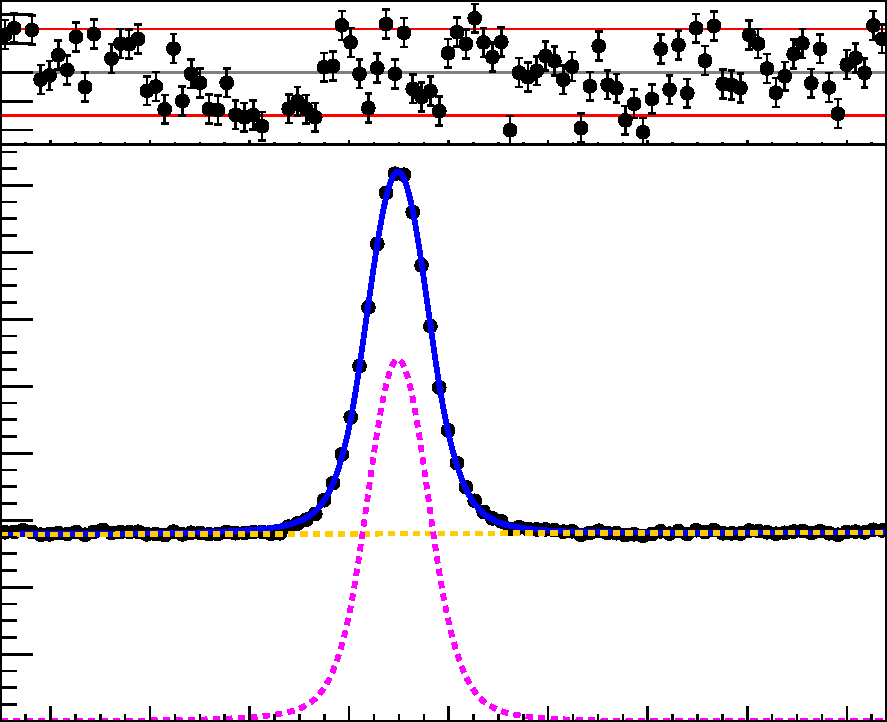
\includegraphics[width=0.9\textwidth]{BsDsK_TD/Time_Resolution/Mfit_ALL}};
        \begin{scope}[x={(image.south east)},y={(image.north west)}]
            \foreach \x in {0, ..., 8}
            {
                \tikzmath{\xpos = (\x / 8) * 0.896 + 0.058; \xtext = 20 * \x + 1900;}
                \node at (\xpos, -0.025) {\(\pgfmathprintnumber[fixed,precision=0,fixed zerofill=true,1000 sep={}]{\xtext}\)};
            }
            \foreach \y in {0, ..., 8}
            {
                \tikzmath{\ypos = (\y / 8) * 0.743; \ytext = 20 * \y;}
                \node[anchor=east] at (0.005, \ypos) {\(\pgfmathprintnumber[fixed,precision=0,fixed zerofill=true]{\ytext}\)};
            }
            \foreach \p in {0, ..., 4}
            {
                \tikzmath{\ypos = (\p / 4) * 0.159 + 0.819; \ptext = (\p - 2) * 2;}
                \node[anchor=east] at (0.005, \ypos) {\(\scriptstyle\pgfmathprintnumber[fixed,precision=0,fixed zerofill=true]{\ptext}\)};
            }
            \node[anchor=south] at (0.03, 1.) {\({\times \num{e2}}\)};
            \node[anchor=east] at (1.0, -0.09) {\({m(\Dspm)}~[\si{\MeVcc}]\)};
            \node[rotate=90,anchor=east,inner xsep=0pt,outer xsep=0pt] at (-0.10, 1.0) {\({\text{Candidates}/(\SI{1.78}{\MeVcc})}\)};
            \node[anchor=west] at (0.06, 0.72) {\Large\lhcb};
        \end{scope}
    \end{tikzpicture}
    \caption{
        Result of the fit to the \KKPi~invariant mass of the prompt sample.}
    \label{fig:BsDsK_TD_Res_sFit_Results}
\end{figure}

From the resulting, statistically pure \Dspm~sample, the resolution of the combination of \Dspm~and random companion track is determined.
The sample is binned in bins of reconstructed per-event decay-time error \dt~(see \cref{tab:BsDsK_TD_Res_Nominal}), and in each bin a double Gaussian shape is effectively fitted to the negative tail of the reconstructed decay time.
The fit takes into account a small range of positive decay-time events in order to correctly model the shape.
The fit model is the sum of two Gaussian functions, where the main part is a narrow Gaussian that accounts for well-measured events and a smaller part is a wider Gaussian for those with a larger uncertainty.
Two example fits are shown in \cref{fig:BsDsK_TD_Res_GaussianFits}.
%
\begin{figure}[hp] \centerfloat
    \fontsize{9}{10.8}\selectfont
    \begin{subfigure}{.8\textwidth} \centerfloat
        \begin{tikzpicture}
            \node[anchor=south west,inner sep=0] (image) at (0,0) {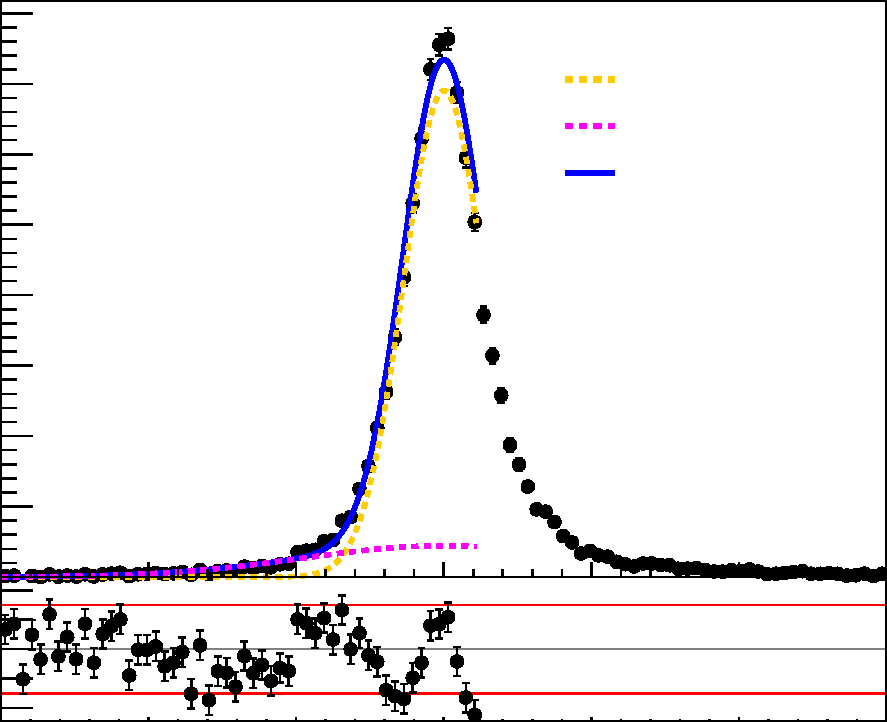
\includegraphics[width=0.9\textwidth]{BsDsK_TD/Time_Resolution/bin002}};
            \begin{scope}[x={(image.south east)},y={(image.north west)}]
                \foreach \x in {0, ..., 6}
                {
                    \tikzmath{\xpos = (\x / 6); \xtext = 100 * \x - 300;}
                    \node at (\xpos, -0.025) {\(\pgfmathprintnumber[fixed,precision=0,fixed zerofill=true]{\xtext}\)};
                }
                \node[anchor=east] at (0.005, .215) {\(0\)};
                \foreach \y in {1, ..., 8}
                {
                    \tikzmath{\ypos = (\y / 8) * 0.777 + .203; \ytext = 500 * \y;}
                    \node[anchor=east] at (0.005, \ypos) {\(\pgfmathprintnumber[fixed,precision=0,fixed zerofill=true,1000 sep={}]{\ytext}\)};
                }
                \foreach \p in {0, ..., 4}
                {
                    \tikzmath{\ypos = (\p / 4) * 0.163 + .02; \ptext = (\p - 2) * 2;}
                    \node[anchor=east] at (0.005, \ypos) {\(\scriptstyle\pgfmathprintnumber[fixed,precision=0,fixed zerofill=true]{\ptext}\)};
                }
                % Legend
                {
                    \node[anchor=base west] at (0.70, 0.876) {Narrow Gaussian};
                    \node[anchor=base west] at (0.70, 0.812) {Wide Gaussian};
                    \node[anchor=base west] at (0.70, 0.748) {Total};
                }
                \node[anchor=east] at (1.0, -0.09) {Decay time~\([\si{\fs}]\)};
                \node[rotate=90,anchor=east,inner xsep=0pt,outer xsep=0pt] at (-0.12, 1.0) {\({\text{Candidates}/(\SI{6.0}{\fs})}\)};
                \node[anchor=west] at (0.06, 0.92) {\Large\lhcb};
            \end{scope}
        \end{tikzpicture}
        \caption{\({\SI{20}{\fs} < \dt < \SI{25}{\fs}}\).}
        \label{fig:BsDsK_TD_Res_GaussianFits_Low}
    \end{subfigure}
    \par\bigskip
    \begin{subfigure}{.8\textwidth} \centerfloat
        \begin{tikzpicture}
            \node[anchor=south west,inner sep=0] (image) at (0,0) {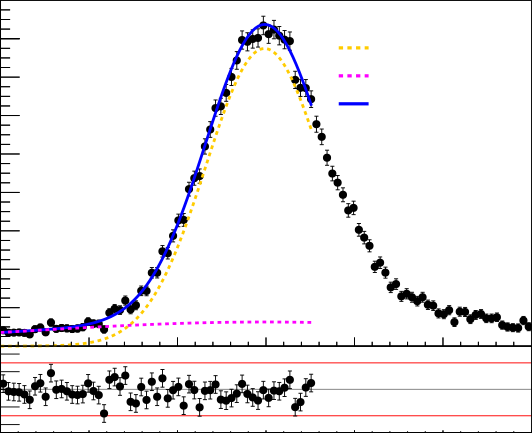
\includegraphics[width=0.9\textwidth]{BsDsK_TD/Time_Resolution/bin017}};
            \begin{scope}[x={(image.south east)},y={(image.north west)}]
                \foreach \x in {0, ..., 6}
                {
                    \tikzmath{\xpos = (\x / 6); \xtext = 100 * \x - 300;}
                    \node at (\xpos, -0.025) {\(\pgfmathprintnumber[fixed,precision=0,fixed zerofill=true]{\xtext}\)};
                }
                \node[anchor=east] at (0.005, .215) {\(0\)};
                \foreach \y in {1, ..., 8}
                {
                    \tikzmath{\ypos = (\y / 8) * 0.708 + .203; \ytext = 200 * \y;}
                    \node[anchor=east] at (0.005, \ypos) {\(\pgfmathprintnumber[fixed,precision=0,fixed zerofill=true,1000 sep={}]{\ytext}\)};
                }
                \foreach \p in {0, ..., 4}
                {
                    \tikzmath{\ypos = (\p / 4) * 0.163 + .02; \ptext = (\p - 2) * 2;}
                    \node[anchor=east] at (0.005, \ypos) {\(\scriptstyle\pgfmathprintnumber[fixed,precision=0,fixed zerofill=true]{\ptext}\)};
                }
                % Legend
                {
                    \node[anchor=base west] at (0.70, 0.876) {Narrow Gaussian};
                    \node[anchor=base west] at (0.70, 0.812) {Wide Gaussian};
                    \node[anchor=base west] at (0.70, 0.748) {Total};
                }
                \node[anchor=east] at (1.0, -0.09) {Decay time~\([\si{\fs}]\)};
                \node[rotate=90,anchor=east,inner xsep=0pt,outer xsep=0pt] at (-0.12, 1.0) {\({\text{Candidates}/(\SI{6.0}{\fs})}\)};
                \node[anchor=west] at (0.06, 0.92) {\Large\lhcb};
            \end{scope}
        \end{tikzpicture}
        \caption{\({\SI{50}{\fs} < \dt \SI{55}{\fs}}\).}
        \label{fig:BsDsK_TD_Res_GaussianFits_High}
    \end{subfigure}
    \caption{
        Fits to the reconstructed decay time of prompt~\Dspm-random track combinations, for two \dt~bins.
        As expected, the lower \dt~bin in~(\subref{fig:BsDsK_TD_Res_GaussianFits_Low}) has a narrower decay-time distribution than the higher bin in~(\subref{fig:BsDsK_TD_Res_GaussianFits_High}).}
    \label{fig:BsDsK_TD_Res_GaussianFits}
\end{figure}

In the decay-time fits later on, a single~Gaussian will be used as resolution model, and therefore the widths of these two Gaussian distributions found here are combined into a single, effective resolution.
To do so, the effect of the resolution on the decay-time distribution of an oscillating \Bs~sample is taken into account.
This effect is characterised by a dilution factor~\(D\), as defined in Ref.~\cite{Moser:1996xf}, which depends on the \Bs~oscillation frequency~\dms.
In case of a double-Gaussian resolution model, the dilution becomes
%
\begin{equation} \label{eqn:BsDsK_TD_Res_Dilution}
    D = f_{1} e^{-\sigma_1^{2} \dmssq / 2} + (1 - f_{1}) e^{-\sigma_{2}^{2} \dmssq / 2} \rlap{,}
\end{equation}
%
where the~\(\sigma_{1,2}\) are the widths of the two Gaussian distributions, and \(f_{1}\)~is the relative fraction of the one corresponding to~\(\sigma_{1}\).
The numerical value of this dimensionless quantity runs between~\num{0}, indicating an infinitely poor decay-time resolution, and~\num{1}, indicating that the resolution has infinite precision.
The inverse of \cref{eqn:BsDsK_TD_Res_Dilution} is used to convert the two resolutions back to a single resolution:
%
\begin{equation} \label{eqn:BsDsK_TD_Res_EffectiveSigma}
    \seff = \sqrt{\dfrac{-2}{\dmssq} \log(D)} \rlap{.}
\end{equation}

It should be noted that this \emph{effective}~resolution is not the actual resolution of the \Bs~sample, but rather a resolution of a single Gaussian that has the same dampening effect on the decay-time distribution as the resolution of a double Gaussian would have.
As such, it can be used in the extraction of the \CP-violation parameters.

The resulting distribution of effective resolutions obtained with the prompts~\Dspm method as a function of per-event decay-time error is shown in \cref{fig:BsDsK_TD_Res_Nominal}, and the used binning scheme and result per bin in \cref{tab:BsDsK_TD_Res_Nominal}.To obtain a continuous dependence on the per-event error, it is parameterised using a linear function, resulting in the following expression:
%
\begin{equation} \label{eqn:BsDsK_TD_Res_Nominal}
    \sigma = s_{0} + s_{1} (\dt - \SI{40}{\fs}) = \SI{61.450 +- 0.380}{\fs} + (\num{1.280 +- 0.042}) (\dt - \SI{40}{\fs}) \rlap{,}
\end{equation}
%
where \(s_{0}\)~and \(s_{1}\)~are the linear parameters and \SI{40}{\fs}~is approximately the average per-event decay-time error in real \BsDsK~events.

\begin{figure}[!htb] \centerfloat
    \begin{tikzpicture}
        \node[anchor=south west,inner sep=0] (image) at (0,0) {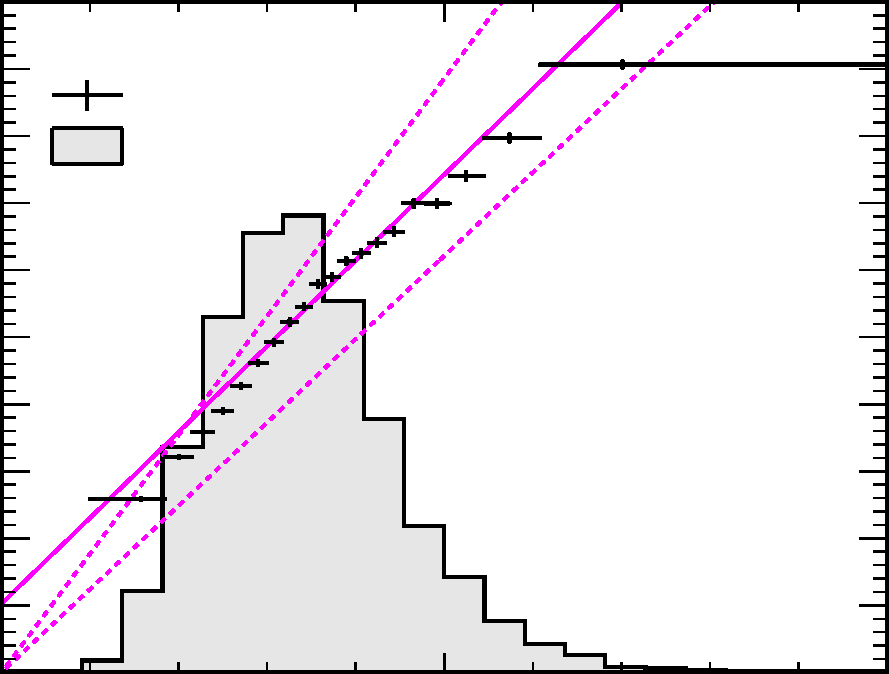
\includegraphics[width=0.9\textwidth]{BsDsK_TD/Time_Resolution/CombinationLinear_ALL_eff_sigma}};
        \begin{scope}[x={(image.south east)},y={(image.north west)}]
            \foreach \x in {0, ..., 10}
            {
                \tikzmath{\xpos = (\x / 10); \xtext = 10 * \x;}
                \node at (\xpos, -0.025) {\(\pgfmathprintnumber[fixed,precision=0,fixed zerofill=true]{\xtext}\)};
            }
            \foreach \y in {0, ..., 10}
            {
                \tikzmath{\ypos = (\y / 10); \ytext = 10 * \y;}
                \node[anchor=east] at (0.005, \ypos) {\(\pgfmathprintnumber[fixed,precision=0,fixed zerofill=true]{\ytext}\)};
            }
            % Legend
            {
                \node[anchor=base west] at (0.14, 0.843) {Prompt~\Dspm data};
                \node[anchor=base west] at (0.14, 0.768) {\BsDsK~data};
            }
            \node[anchor=east] at (1.0, -0.09) {Per-event decay-time error~\dt~\([\si{\fs}]\)};
            \node[rotate=90,anchor=east,inner xsep=0pt,outer xsep=0pt] at (-0.12, 1.0) {Decay-time resolution~\({\sigma~[\si{\fs}]}\)};
            \node[anchor=west] at (0.06, 0.92) {\Large\lhcb};
        \end{scope}
    \end{tikzpicture}
    \caption{
        Measured resolution in bins of the per-event decay-time error (data points) and results of the fit according to the expression in \cref{eqn:BsDsK_TD_Res_Nominal} (solid line).
        The histogram shows the distribution of per-event errors of the \BsDsK~sample with weights from the multivariate fit applied.
        The dashed lines are the relations used to evaluate systematic effects (see \cref{sec:BsDsK_TD_Res_Syst}).}
    \label{fig:BsDsK_TD_Res_Nominal}
\end{figure}
%
\begin{table}[!htb] \centerfloat
    \caption{
        Measured resolution in bins of the per-event decay-time error.}
    \label{tab:BsDsK_TD_Res_Nominal}
    \hspace*{-.75cm}
    \rowcolors{3}{tableshade}{}
    \sisetup{table-number-alignment=right}
    \begin{tabular}{cS[table-format=2.1(1)]cS[table-format=1.2(2)]S[table-format=1.2(1)]S[table-format=2.1(1)]}
        \hiderowcolors \toprule
        \multirow{2}{*}[-2pt]{\dt~bin~(\si{\fs})} & \multicolumn{5}{c}{Double-Gaussian fit results} \tabularnewline
        \cmidrule(lr){2-6}
                             & {\(\sigma_{1}\)~(\si{\fs})} & \(\sigma_{2}\)~(\si{\fs}) & {\(f\)} & {\(D\)} & {\(\seff\)~(\si{\fs})} \tabularnewline
        \showrowcolors \midrule
        \(\09.2\,-\,\018.5\) & 18.1 +- 0.0 & \(\076\,\pm\,\01\) & 0.85 +- 0.0 & 0.86 +- 0.0 & 29.8 +- 0.1 \tabularnewline
        \( 18.5\,-\,\021.5\) & 24.2 +- 0.3 & \(\089\,\pm\,\02\) & 0.85 +- 0.0 & 0.82 +- 0.0 & 35.0 +- 0.2 \tabularnewline
        \( 21.5\,-\,\023.9\) & 27.4 +- 0.3 & \(\094\,\pm\,\02\) & 0.85 +- 0.0 & 0.79 +- 0.0 & 38.0 +- 0.2 \tabularnewline
        \( 23.9\,-\,\026.0\) & 31.3 +- 0.4 & \( 103\,\pm\,\02\) & 0.87 +- 0.0 & 0.76 +- 0.0 & 40.7 +- 0.2 \tabularnewline
        \( 26.0\,-\,\028.0\) & 33.6 +- 0.4 & \( 112\,\pm\,\03\) & 0.85 +- 0.0 & 0.73 +- 0.0 & 44.2 +- 0.3 \tabularnewline
        \( 28.0\,-\,\029.9\) & 36.0 +- 0.5 & \( 113\,\pm\,\03\) & 0.83 +- 0.0 & 0.70 +- 0.0 & 47.1 +- 0.3 \tabularnewline
        \( 29.9\,-\,\031.7\) & 38.5 +- 0.5 & \( 117\,\pm\,\03\) & 0.83 +- 0.0 & 0.67 +- 0.0 & 49.7 +- 0.3 \tabularnewline
        \( 31.7\,-\,\033.4\) & 39.9 +- 0.6 & \( 113\,\pm\,\03\) & 0.79 +- 0.0 & 0.64 +- 0.0 & 52.4 +- 0.3 \tabularnewline
        \( 33.4\,-\,\035.0\) & 38.7 +- 0.6 & \( 111\,\pm\,\02\) & 0.74 +- 0.0 & 0.62 +- 0.0 & 54.6 +- 0.3 \tabularnewline
        \( 35.0\,-\,\036.6\) & 43.8 +- 0.6 & \( 135\,\pm\,\04\) & 0.78 +- 0.0 & 0.58 +- 0.0 & 57.9 +- 0.4 \tabularnewline
        \( 36.6\,-\,\038.1\) & 44.9 +- 0.7 & \( 122\,\pm\,\03\) & 0.76 +- 0.0 & 0.57 +- 0.0 & 59.0 +- 0.4 \tabularnewline
        \( 38.1\,-\,\039.8\) & 49.4 +- 0.8 & \( 174\,\pm\,\07\) & 0.80 +- 0.0 & 0.55 +- 0.0 & 61.3 +- 0.4 \tabularnewline
        \( 39.8\,-\,\041.5\) & 51.9 +- 0.7 & \( 196\,\pm\, 10\) & 0.82 +- 0.0 & 0.53 +- 0.0 & 62.5 +- 0.5 \tabularnewline
        \( 41.5\,-\,\043.3\) & 51.1 +- 0.7 & \( 164\,\pm\,\06\) & 0.78 +- 0.0 & 0.52 +- 0.0 & 64.0 +- 0.4 \tabularnewline
        \( 43.3\,-\,\045.4\) & 52.6 +- 0.7 & \( 179\,\pm\,\08\) & 0.78 +- 0.0 & 0.50 +- 0.0 & 65.7 +- 0.4 \tabularnewline
        \( 45.4\,-\,\047.7\) & 58.9 +- 0.9 & \( 188\,\pm\, 10\) & 0.79 +- 0.0 & 0.46 +- 0.0 & 69.9 +- 0.5 \tabularnewline
        \( 47.7\,-\,\050.6\) & 58.9 +- 0.9 & \( 197\,\pm\, 11\) & 0.79 +- 0.0 & 0.46 +- 0.0 & 69.9 +- 0.5 \tabularnewline
        \( 50.6\,-\,\054.5\) & 66.3 +- 1.0 & \( 279\,\pm\, 38\) & 0.84 +- 0.0 & 0.42 +- 0.0 & 74.0 +- 0.5 \tabularnewline
        \( 54.5\,-\,\060.8\) & 70.4 +- 1.2 & \( 197\,\pm\, 15\) & 0.80 +- 0.0 & 0.36 +- 0.0 & 79.7 +- 0.6 \tabularnewline
        \( 60.8\,-\, 150.0\) & 82.5 +- 1.4 & \( 253\,\pm\, 38\) & 0.80 +- 0.0 & 0.27 +- 0.0 & 90.6 +- 0.5 \tabularnewline
        \bottomrule
    \end{tabular}
\end{table}

\clearpage
\subsection{Validation}

The procedure to calibrate the per-event decay-time error to match the decay-time resolution is validated in several ways:
%
\begin{itemize}
    \item by comparing the measured resolution on simulated prompt \Dspm~candidates combined with a random companion track, to the actual resolution of simulated \Bs~candidates;
    \item by investigating the dependence of the resolution on the kinematic differences between prompt~\Dspm~events and \BsDsK~events;
    \item by verifying that the resolution does not depend on the \Bs~decay time.
\end{itemize}
%
The first validation is obtained from a sample of simulated \BsDsK~events, in the same manner as for data.
This simulated sample is processed as described in \cref{sec:stripping}, except the requirement on decay time is removed.
The result is
%
\begin{equation} \label{eqn:BsDsK_TD_Res_MC}
    \sigma_{\text{MC}} = s_{0} + s_{1} (\dt - \SI{40}{\fs}) = (\num{1.201 +- 0.013})\dt \rlap{,}
\end{equation}
%
with the constant term compatible with, and hence fixed to, zero.
This justifies directly fitting the pull distribution, \ie~the distribution of~\(t/\dt\), to determine the scale factor, which quantifies the difference between the calculated per-event error and the measured resolution.
This fit consists of a single Gaussian function, where the width of that function represents the scale factor.
The result, \num{1.215 +- 0.006}, is consistent with \cref{eqn:BsDsK_TD_Res_MC}.
Additionally, the scale factor is determined for a sample of simulated prompt \Dspm~decays, matching those used in \cref{sec:BsDsK_TD_Res_Calib}.
The size of this sample is insufficient to perform the analysis in bins of the per-event decay-time errors, and therefore only the scale factor is determined.
The fits and scale factors of both samples are shown in \cref{tab:BsDsK_TD_Res_MC,fig:BsDsK_TD_Res_MC}.
From these results, it can be seen that the scale factors agree between the prompt~\Dspm and \Bs~simulated samples.
Therefore, it is concluded that the prompt \Dspm~sample serves as a valid proxy for the resolution on \BsDsK~candidates.
%
\begin{table}[htb] \centerfloat
    \caption{
        Results of the Gaussian fits to the pull distribution,~\(t/\dt\), of simulated samples.}
    \label{tab:BsDsK_TD_Res_MC}
    \sisetup{table-number-alignment=right}
    \begin{tabular}{lS[table-format=1.3(3)]}
        \toprule
        Sample       & {Width} \tabularnewline
        \midrule
        \BsDsK       & 1.215 +- 0.006 \tabularnewline
        Prompt~\Dspm & 1.189 +- 0.014 \tabularnewline
        \bottomrule
    \end{tabular}
\end{table}
%
\begin{figure}[hp] \centerfloat
    \fontsize{9}{10.8}\selectfont
    \begin{subfigure}{.8\textwidth} \centerfloat
        \begin{tikzpicture}
            \node[anchor=south west,inner sep=0] (image) at (0,0) {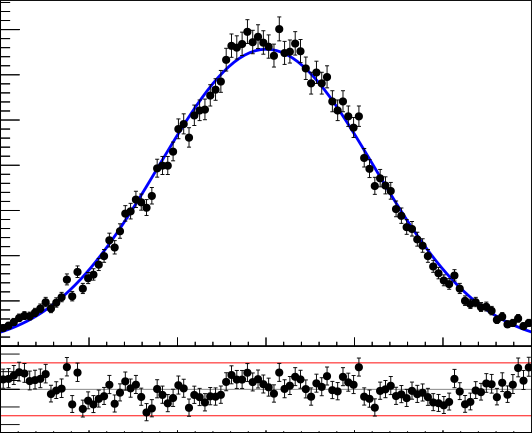
\includegraphics[width=0.9\textwidth]{BsDsK_TD/Time_Resolution/Fit_Pull_DsK_MC_LTUB}};
            \begin{scope}[x={(image.south east)},y={(image.north west)}]
                \foreach \x in {0, ..., 6}
                {
                    \tikzmath{\xpos = (\x / 6); \xtext = \x - 3;}
                    \node at (\xpos, -0.025) {\(\pgfmathprintnumber[fixed,precision=0,fixed zerofill=true]{\xtext}\)};
                }
                \node[anchor=east] at (0.005, .215) {\(0\)};
                \foreach \y in {1, ..., 7}
                {
                    \tikzmath{\ypos = (\y / 7) * 0.729 + .203; \ytext = 100 * \y;}
                    \node[anchor=east] at (0.005, \ypos) {\(\pgfmathprintnumber[fixed,precision=0,fixed zerofill=true,1000 sep={}]{\ytext}\)};
                }
                \foreach \p in {0, ..., 4}
                {
                    \tikzmath{\ypos = (\p / 4) * 0.163 + .02; \ptext = (\p - 2) * 2;}
                    \node[anchor=east] at (0.005, \ypos) {\(\scriptstyle\pgfmathprintnumber[fixed,precision=0,fixed zerofill=true]{\ptext}\)};
                }
                \node[anchor=east] at (1.0, -0.08) {\({t/\dt}\)};
                \node[rotate=90,anchor=east,inner xsep=0pt,outer xsep=0pt] at (-0.12, 1.0) {\({\text{Candidates}/0.06}\)};
                \node[anchor=west] at (0.06, 0.92) {\Large\lhcb};
            \end{scope}
        \end{tikzpicture}
        \caption{Simulated \BsDsK~events.}
    \end{subfigure}
    \par\bigskip
    \begin{subfigure}{.8\textwidth} \centerfloat
        \begin{tikzpicture}
            \node[anchor=south west,inner sep=0] (image) at (0,0) {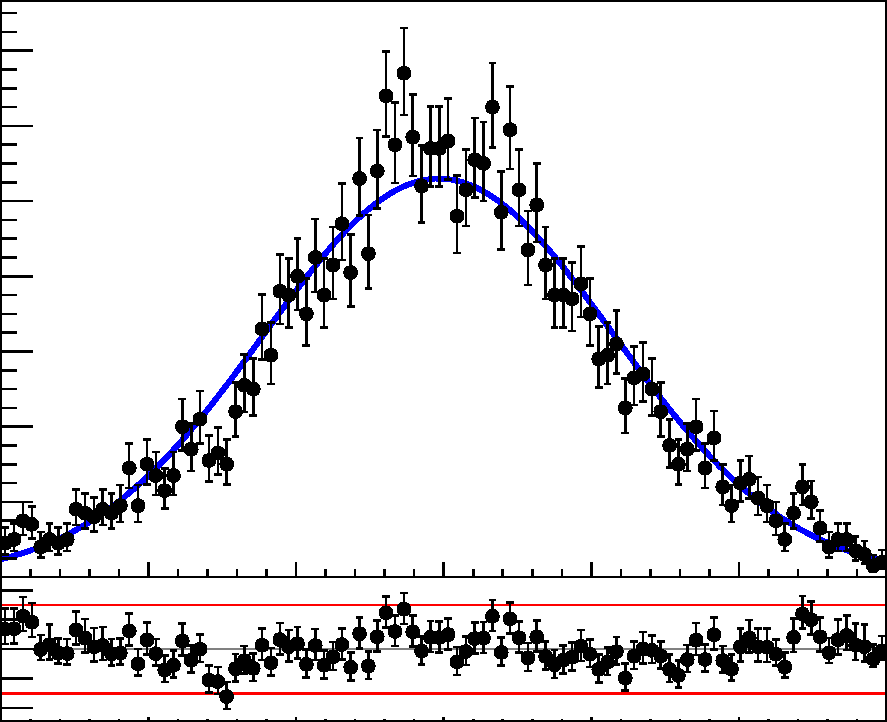
\includegraphics[width=0.9\textwidth]{BsDsK_TD/Time_Resolution/Fit_Pull_Ds_MC}};
            \begin{scope}[x={(image.south east)},y={(image.north west)}]
                \foreach \x in {0, ..., 6}
                {
                    \tikzmath{\xpos = (\x / 6); \xtext = \x - 3;}
                    \node at (\xpos, -0.025) {\(\pgfmathprintnumber[fixed,precision=0,fixed zerofill=true]{\xtext}\)};
                }
                \node[anchor=east] at (0.005, .215) {\(0\)};
                \foreach \y in {1, ..., 7}
                {
                    \tikzmath{\ypos = (\y / 7) * 0.726 + .203; \ytext = 20 * \y;}
                    \node[anchor=east] at (0.005, \ypos) {\(\pgfmathprintnumber[fixed,precision=0,fixed zerofill=true,1000 sep={}]{\ytext}\)};
                }
                \foreach \p in {0, ..., 4}
                {
                    \tikzmath{\ypos = (\p / 4) * 0.163 + .02; \ptext = (\p - 2) * 2;}
                    \node[anchor=east] at (0.005, \ypos) {\(\scriptstyle\pgfmathprintnumber[fixed,precision=0,fixed zerofill=true]{\ptext}\)};
                }
                \node[anchor=east] at (1.0, -0.08) {\({t/\dt}\)};
                \node[rotate=90,anchor=east,inner xsep=0pt,outer xsep=0pt] at (-0.12, 1.0) {\({\text{Candidates}/0.06}\)};
                \node[anchor=west] at (0.06, 0.92) {\Large\lhcb};
            \end{scope}
        \end{tikzpicture}
        \caption{Simulated prompt~\Dspm~events.}
    \end{subfigure}
    \caption{
        Gaussian fits to the \(t/\dt\)~distributions of simulated~\BsDsK events and simulated prompt~\Dspm events.}
    \label{fig:BsDsK_TD_Res_MC}
\end{figure}

Possible differences between these samples is further investigated by inspecting the dependence of the decay-time resolution on the kinematic variable in which prompt~\Dspm and signal \Bs~decays differ the most.
This variable is the companion track~\pt, and to determine this dependence the prompt~\Dspm sample is binned in this variable, after which the same procedure is used to determine the decay-time resolution in each of those bins.
The result of this binned analysis is shown in \cref{fig:BsDsK_TD_Res_PtBins,tab:BsDsK_TD_Res_PtBins}, the latter of which also contains the used binning scheme.
The results show no significant \pt~dependence, except for the highest bin, where low statistics interfere with the determination of~\(s_{0}\) and~\(s_{1}\). 
%
\begin{table}[hb] \centerfloat
    \caption{
        Decay-time resolution corrections of the prompt~\Dspm data sample, in bins of the companion track~\pt.}
    \label{tab:BsDsK_TD_Res_PtBins}
    \rowcolors{2}{tableshade}{}
    \begin{tabular}{cS[table-format=2.1(1)]S[table-format=1.3(3)]}
        \toprule
        \(\pt\)~(\si{\MeVc}) & {\(s_{0}\)~(\si{\fs})} & {\(s_{1}\)} \tabularnewline
        \midrule
        \(\0500\,-\,\0850\) & 59.7 +- 0.4 & 1.239 +- 0.045 \tabularnewline
        \(\0850\,-\, 1150\) & 60.8 +- 0.4 & 1.292 +- 0.047 \tabularnewline
        \( 1150\,-\, 1600\) & 60.3 +- 0.4 & 1.247 +- 0.047 \tabularnewline
        \( 1600\,-\, 2500\) & 63.8 +- 0.5 & 1.388 +- 0.059 \tabularnewline
        \aligncell{r}{\(> \num{2500}\)} & 74.7 +- 1.0 & 2.222 +- 0.106 \tabularnewline
        \bottomrule
    \end{tabular}
\end{table}
%
\begin{figure}[p] \centerfloat
    \fontsize{7}{8.4}\selectfont
    \begin{subfigure}{.48\textwidth} \centerfloat
        \begin{tikzpicture}
            \node[anchor=south west,inner sep=0] (image) at (0,0) {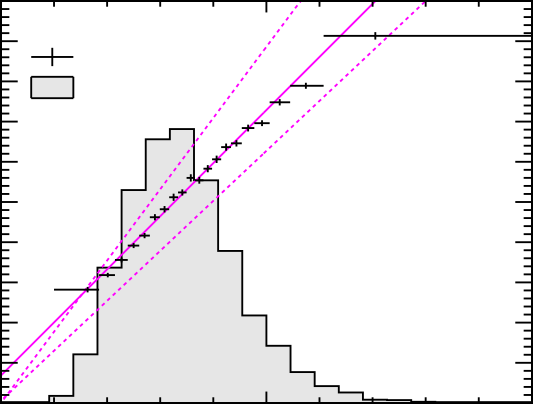
\includegraphics[width=0.9\textwidth]{BsDsK_TD/Time_Resolution/CombinationLinear_ALL_PtBin00_eff_sigma}};
            \begin{scope}[x={(image.south east)},y={(image.north west)}]
                \foreach \x in {0, ..., 10}
                {
                    \tikzmath{\xpos = (\x / 10); \xtext = 10 * \x;}
                    \node at (\xpos, -0.033) {\(\pgfmathprintnumber[fixed,precision=0,fixed zerofill=true]{\xtext}\)};
                }
                \foreach \y in {0, ..., 10}
                {
                    \tikzmath{\ypos = (\y / 10); \ytext = 10 * \y;}
                    \node[anchor=east] at (0.005, \ypos) {\(\pgfmathprintnumber[fixed,precision=0,fixed zerofill=true]{\ytext}\)};
                }
                % Legend
                {
                    \fontsize{6}{7.2}\selectfont
                    \node[anchor=base west] at (0.14, 0.843) {Prompt~\Dspm data};
                    \node[anchor=base west] at (0.14, 0.768) {\BsDsK};
                    \node[anchor=base west] at (0.14, 0.708) {data};
                }
                \node[anchor=east] at (1.0, -0.10) {Per-event decay-time error~\dt~\([\si{\fs}]\)};
                \node[rotate=90,anchor=east,inner xsep=0pt,outer xsep=0pt] at (-0.12, 1.0) {Decay-time resolution~\({\sigma~[\si{\fs}]}\)};
                \node[anchor=west] at (0.055, 0.94) {\fontsize{10}{12}\selectfont \lhcb};
            \end{scope}
        \end{tikzpicture}
        \caption{\(500<\pt/(\si{\MeVc})< 850\)\rlap{.}}
    \end{subfigure} \hfill%
    \begin{subfigure}{.48\textwidth} \centerfloat
        \begin{tikzpicture}
            \node[anchor=south west,inner sep=0] (image) at (0,0) {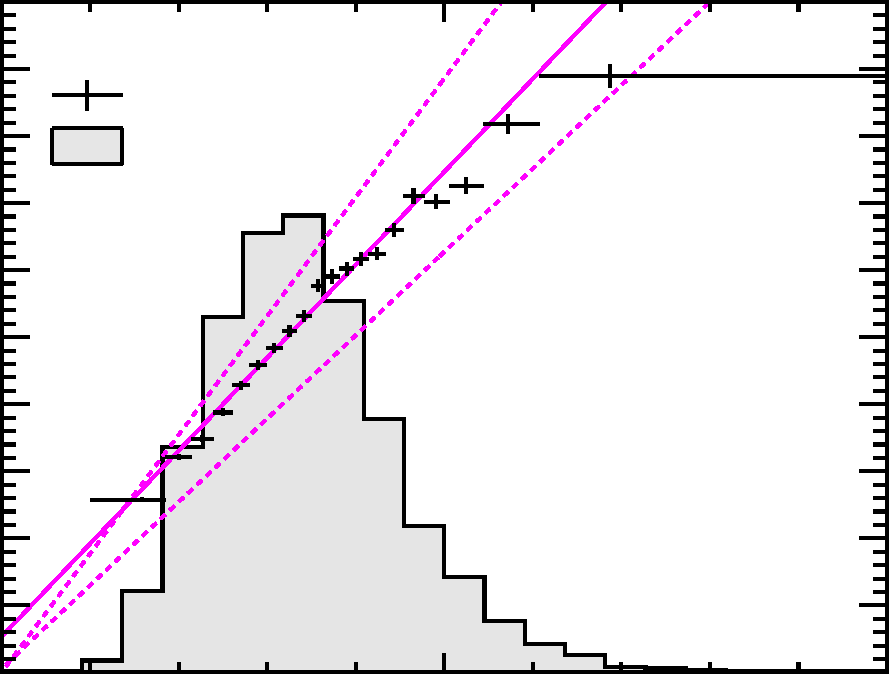
\includegraphics[width=0.9\textwidth]{BsDsK_TD/Time_Resolution/CombinationLinear_ALL_PtBin01_eff_sigma}};
            \begin{scope}[x={(image.south east)},y={(image.north west)}]
                \foreach \x in {0, ..., 10}
                {
                    \tikzmath{\xpos = (\x / 10); \xtext = 10 * \x;}
                    \node at (\xpos, -0.033) {\(\pgfmathprintnumber[fixed,precision=0,fixed zerofill=true]{\xtext}\)};
                }
                \foreach \y in {0, ..., 10}
                {
                    \tikzmath{\ypos = (\y / 10); \ytext = 10 * \y;}
                    \node[anchor=east] at (0.005, \ypos) {\(\pgfmathprintnumber[fixed,precision=0,fixed zerofill=true]{\ytext}\)};
                }
                % Legend
                {
                    \fontsize{6}{7.2}\selectfont
                    \node[anchor=base west] at (0.14, 0.843) {Prompt~\Dspm data};
                    \node[anchor=base west] at (0.14, 0.768) {\BsDsK};
                    \node[anchor=base west] at (0.14, 0.708) {data};
                }
                \node[anchor=east] at (1.0, -0.10) {Per-event decay-time error~\dt~\([\si{\fs}]\)};
                \node[rotate=90,anchor=east,inner xsep=0pt,outer xsep=0pt] at (-0.12, 1.0) {Decay-time resolution~\({\sigma~[\si{\fs}]}\)};
                \node[anchor=west] at (0.055, 0.94) {\fontsize{10}{12}\selectfont \lhcb};
            \end{scope}
        \end{tikzpicture}
        \caption{\(850<\pt/(\si{\MeVc})<1150\)\rlap{.}}
    \end{subfigure}
    \par\bigskip
    \begin{subfigure}{.48\textwidth} \centerfloat
        \begin{tikzpicture}
            \node[anchor=south west,inner sep=0] (image) at (0,0) {\includegraphics[width=0.9\textwidth]{BsDsK_TD/Time_Resolution/CombinationLinear_ALL_PtBin02_eff_sigma}};
            \begin{scope}[x={(image.south east)},y={(image.north west)}]
                \foreach \x in {0, ..., 10}
                {
                    \tikzmath{\xpos = (\x / 10); \xtext = 10 * \x;}
                    \node at (\xpos, -0.033) {\(\pgfmathprintnumber[fixed,precision=0,fixed zerofill=true]{\xtext}\)};
                }
                \foreach \y in {0, ..., 10}
                {
                    \tikzmath{\ypos = (\y / 10); \ytext = 10 * \y;}
                    \node[anchor=east] at (0.005, \ypos) {\(\pgfmathprintnumber[fixed,precision=0,fixed zerofill=true]{\ytext}\)};
                }
                % Legend
                {
                    \fontsize{6}{7.2}\selectfont
                    \node[anchor=base west] at (0.14, 0.843) {Prompt~\Dspm data};
                    \node[anchor=base west] at (0.14, 0.768) {\BsDsK};
                    \node[anchor=base west] at (0.14, 0.708) {data};
                }
                \node[anchor=east] at (1.0, -0.10) {Per-event decay-time error~\dt~\([\si{\fs}]\)};
                \node[rotate=90,anchor=east,inner xsep=0pt,outer xsep=0pt] at (-0.12, 1.0) {Decay-time resolution~\({\sigma~[\si{\fs}]}\)};
                \node[anchor=west] at (0.055, 0.94) {\fontsize{10}{12}\selectfont \lhcb};
            \end{scope}
        \end{tikzpicture}
        \caption{\(1150<\pt/(\si{\MeVc})<1600\)\rlap{.}}
    \end{subfigure}
    \par\bigskip
    \begin{subfigure}{.48\textwidth} \centerfloat
        \begin{tikzpicture}
            \node[anchor=south west,inner sep=0] (image) at (0,0) {\includegraphics[width=0.9\textwidth]{BsDsK_TD/Time_Resolution/CombinationLinear_ALL_PtBin03_eff_sigma}};
            \begin{scope}[x={(image.south east)},y={(image.north west)}]
                \foreach \x in {0, ..., 10}
                {
                    \tikzmath{\xpos = (\x / 10); \xtext = 10 * \x;}
                    \node at (\xpos, -0.033) {\(\pgfmathprintnumber[fixed,precision=0,fixed zerofill=true]{\xtext}\)};
                }
                \foreach \y in {0, ..., 10}
                {
                    \tikzmath{\ypos = (\y / 10); \ytext = 10 * \y;}
                    \node[anchor=east] at (0.005, \ypos) {\(\pgfmathprintnumber[fixed,precision=0,fixed zerofill=true]{\ytext}\)};
                }
                % Legend
                {
                    \fontsize{6}{7.2}\selectfont
                    \node[anchor=base west] at (0.14, 0.843) {Prompt~\Dspm data};
                    \node[anchor=base west] at (0.14, 0.768) {\BsDsK};
                    \node[anchor=base west] at (0.14, 0.708) {data};
                }
                \node[anchor=east] at (1.0, -0.10) {Per-event decay-time error~\dt~\([\si{\fs}]\)};
                \node[rotate=90,anchor=east,inner xsep=0pt,outer xsep=0pt] at (-0.12, 1.0) {Decay-time resolution~\({\sigma~[\si{\fs}]}\)};
                \node[anchor=west] at (0.055, 0.94) {\fontsize{10}{12}\selectfont \lhcb};
            \end{scope}
        \end{tikzpicture}
        \caption{\(1600<\pt/(\si{\MeVc})<2500\)\rlap{.}}
    \end{subfigure} \hfill%
    \begin{subfigure}{.48\textwidth} \centerfloat
        \begin{tikzpicture}
            \node[anchor=south west,inner sep=0] (image) at (0,0) {\includegraphics[width=0.9\textwidth]{BsDsK_TD/Time_Resolution/CombinationLinear_ALL_PtBin04_eff_sigma}};
            \begin{scope}[x={(image.south east)},y={(image.north west)}]
                \foreach \x in {0, ..., 10}
                {
                    \tikzmath{\xpos = (\x / 10); \xtext = 10 * \x;}
                    \node at (\xpos, -0.033) {\(\pgfmathprintnumber[fixed,precision=0,fixed zerofill=true]{\xtext}\)};
                }
                \foreach \y in {0, ..., 10}
                {
                    \tikzmath{\ypos = (\y / 10); \ytext = 10 * \y;}
                    \node[anchor=east] at (0.005, \ypos) {\(\pgfmathprintnumber[fixed,precision=0,fixed zerofill=true]{\ytext}\)};
                }
                \node[anchor=east] at (1.0, -0.10) {Per-event decay-time error~\dt~\([\si{\fs}]\)};
                \node[rotate=90,anchor=east,inner xsep=0pt,outer xsep=0pt] at (-0.12, 1.0) {Decay-time resolution~\({\sigma~[\si{\fs}]}\)};
                \node[anchor=west] at (0.055, 0.94) {\fontsize{10}{12}\selectfont \lhcb};
            \end{scope}
        \end{tikzpicture}
        \caption{\(\pt>\SI{2500}{\MeVc}\)\rlap{.}}
    \end{subfigure}
    \caption{
        Measured resolution of the prompt~\Dspm data sample, split in five bins of companion track~\pt.}
    \label{fig:BsDsK_TD_Res_PtBins}
\end{figure}

\clearpage

The final validation checks the dependence of the resolution on the \Bs~decay time.
Since the prompt \Dspm~sample only consists of candidates with true decay time zero, it is unsuitable to verify this dependence.
Rather, it is performed on the sample of simulated \BsDsK~events introduced above.
The results are shown in \cref{fig:BsDsK_TD_Res_tBins,tab:BsDsK_TD_Res_tBins}.
All values are compatible with the result in \cref{tab:BsDsK_TD_Res_MC}, and the resolution is found not to depend on the \Bs~decay time.
%
\begin{table}[hb] \centerfloat
    \caption{
        Results of the decay-time resolution determinations on simulated \BsDsK~events in bins of the \Bs~candidate decay time, using both a linear fit with the constant term fixed to zero.}
    \label{tab:BsDsK_TD_Res_tBins}
    \rowcolors{2}{tableshade}{}
    \begin{tabular}{cS[table-format=1.3(3)]S[table-format=2.1(1)]S[table-format=1.3(3)]}
        \toprule
        \(t~(\si{\ps})\)     & {\(s_{1}\)}    & \tabularnewline
        \midrule
        \(0\z\0\,-\,\00.5\)  & 1.178 +- 0.032 & \tabularnewline
        \(  0.5\,-\,\00.8\)  & 1.185 +- 0.021 & \tabularnewline
        \(  0.8\,-\,\01.5\)  & 1.204 +- 0.024 & \tabularnewline
        \(  1.5\,-\,\02.5\)  & 1.196 +- 0.026 & \tabularnewline
        \(  2.5\,-\,10\z\0\) & 1.189 +- 0.020 & \tabularnewline
        \bottomrule
    \end{tabular}
\end{table}
%
\begin{figure}[p] \centerfloat
    \fontsize{7}{8.4}\selectfont
    \begin{subfigure}{.48\textwidth} \centerfloat
        \begin{tikzpicture}
            \node[anchor=south west,inner sep=0] (image) at (0,0) {\includegraphics[width=0.9\textwidth]{BsDsK_TD/Time_Resolution/CombinationLinear_DsK_MC_LTUB_TrecBin00_eff_sigma}};
            \begin{scope}[x={(image.south east)},y={(image.north west)}]
                \foreach \x in {0, ..., 10}
                {
                    \tikzmath{\xpos = (\x / 10); \xtext = 10 * \x;}
                    \node at (\xpos, -0.033) {\(\pgfmathprintnumber[fixed,precision=0,fixed zerofill=true]{\xtext}\)};
                }
                \foreach \y in {0, ..., 10}
                {
                    \tikzmath{\ypos = (\y / 10); \ytext = 10 * \y;}
                    \node[anchor=east] at (0.005, \ypos) {\(\pgfmathprintnumber[fixed,precision=0,fixed zerofill=true]{\ytext}\)};
                }
                % Legend
                {
                    \fontsize{6}{7.2}\selectfont
                    \node[anchor=base west] at (0.14, 0.843) {Simulated~data};
                    \node[anchor=base west] at (0.14, 0.768) {\BsDsK};
                    \node[anchor=base west] at (0.14, 0.708) {data};
                }
                \node[anchor=east] at (1.0, -0.10) {Per-event decay-time error~\dt~\([\si{\fs}]\)};
                \node[rotate=90,anchor=east,inner xsep=0pt,outer xsep=0pt] at (-0.12, 1.0) {Decay-time resolution~\({\sigma~[\si{\fs}]}\)};
                \node[anchor=west] at (0.055, 0.94) {\fontsize{10}{12}\selectfont \lhcb};
            \end{scope}
        \end{tikzpicture}
        \caption{\(0<t/\si{\ps}<0.5\)\rlap{.}}
    \end{subfigure} \hfill%
    \begin{subfigure}{.48\textwidth} \centerfloat
        \begin{tikzpicture}
            \node[anchor=south west,inner sep=0] (image) at (0,0) {\includegraphics[width=0.9\textwidth]{BsDsK_TD/Time_Resolution/CombinationLinear_DsK_MC_LTUB_TrecBin01_eff_sigma}};
            \begin{scope}[x={(image.south east)},y={(image.north west)}]
                \foreach \x in {0, ..., 10}
                {
                    \tikzmath{\xpos = (\x / 10); \xtext = 10 * \x;}
                    \node at (\xpos, -0.033) {\(\pgfmathprintnumber[fixed,precision=0,fixed zerofill=true]{\xtext}\)};
                }
                \foreach \y in {0, ..., 10}
                {
                    \tikzmath{\ypos = (\y / 10); \ytext = 10 * \y;}
                    \node[anchor=east] at (0.005, \ypos) {\(\pgfmathprintnumber[fixed,precision=0,fixed zerofill=true]{\ytext}\)};
                }
                % Legend
                {
                    \fontsize{6}{7.2}\selectfont
                    \node[anchor=base west] at (0.14, 0.843) {Simulated~data};
                    \node[anchor=base west] at (0.14, 0.768) {\BsDsK};
                    \node[anchor=base west] at (0.14, 0.708) {data};
                }
                \node[anchor=east] at (1.0, -0.10) {Per-event decay-time error~\dt~\([\si{\fs}]\)};
                \node[rotate=90,anchor=east,inner xsep=0pt,outer xsep=0pt] at (-0.12, 1.0) {Decay-time resolution~\({\sigma~[\si{\fs}]}\)};
                \node[anchor=west] at (0.055, 0.94) {\fontsize{10}{12}\selectfont \lhcb};
            \end{scope}
        \end{tikzpicture}
        \caption{\(0.5<t/\si{\ps}<0.8\)\rlap{.}}
    \end{subfigure}
    \par\bigskip
    \begin{subfigure}{.48\textwidth} \centerfloat
        \begin{tikzpicture}
            \node[anchor=south west,inner sep=0] (image) at (0,0) {\includegraphics[width=0.9\textwidth]{BsDsK_TD/Time_Resolution/CombinationLinear_DsK_MC_LTUB_TrecBin02_eff_sigma}};
            \begin{scope}[x={(image.south east)},y={(image.north west)}]
                \foreach \x in {0, ..., 10}
                {
                    \tikzmath{\xpos = (\x / 10); \xtext = 10 * \x;}
                    \node at (\xpos, -0.033) {\(\pgfmathprintnumber[fixed,precision=0,fixed zerofill=true]{\xtext}\)};
                }
                \foreach \y in {0, ..., 10}
                {
                    \tikzmath{\ypos = (\y / 10); \ytext = 10 * \y;}
                    \node[anchor=east] at (0.005, \ypos) {\(\pgfmathprintnumber[fixed,precision=0,fixed zerofill=true]{\ytext}\)};
                }
                % Legend
                {
                    \fontsize{6}{7.2}\selectfont
                    \node[anchor=base west] at (0.14, 0.843) {Simulated~data};
                    \node[anchor=base west] at (0.14, 0.768) {\BsDsK};
                    \node[anchor=base west] at (0.14, 0.708) {data};
                }
                \node[anchor=east] at (1.0, -0.10) {Per-event decay-time error~\dt~\([\si{\fs}]\)};
                \node[rotate=90,anchor=east,inner xsep=0pt,outer xsep=0pt] at (-0.12, 1.0) {Decay-time resolution~\({\sigma~[\si{\fs}]}\)};
                \node[anchor=west] at (0.055, 0.94) {\fontsize{10}{12}\selectfont \lhcb};
            \end{scope}
        \end{tikzpicture}
        \caption{\(0.8<t/\si{\ps}<1.5\)\rlap{.}}
    \end{subfigure}
    \par\bigskip
    \begin{subfigure}{.48\textwidth} \centerfloat
        \begin{tikzpicture}
            \node[anchor=south west,inner sep=0] (image) at (0,0) {\includegraphics[width=0.9\textwidth]{BsDsK_TD/Time_Resolution/CombinationLinear_DsK_MC_LTUB_TrecBin03_eff_sigma}};
            \begin{scope}[x={(image.south east)},y={(image.north west)}]
                \foreach \x in {0, ..., 10}
                {
                    \tikzmath{\xpos = (\x / 10); \xtext = 10 * \x;}
                    \node at (\xpos, -0.033) {\(\pgfmathprintnumber[fixed,precision=0,fixed zerofill=true]{\xtext}\)};
                }
                \foreach \y in {0, ..., 10}
                {
                    \tikzmath{\ypos = (\y / 10); \ytext = 10 * \y;}
                    \node[anchor=east] at (0.005, \ypos) {\(\pgfmathprintnumber[fixed,precision=0,fixed zerofill=true]{\ytext}\)};
                }
                % Legend
                {
                    \fontsize{6}{7.2}\selectfont
                    \node[anchor=base west] at (0.14, 0.843) {Simulated~data};
                    \node[anchor=base west] at (0.14, 0.768) {\BsDsK};
                    \node[anchor=base west] at (0.14, 0.708) {data};
                }
                \node[anchor=east] at (1.0, -0.10) {Per-event decay-time error~\dt~\([\si{\fs}]\)};
                \node[rotate=90,anchor=east,inner xsep=0pt,outer xsep=0pt] at (-0.12, 1.0) {Decay-time resolution~\({\sigma~[\si{\fs}]}\)};
                \node[anchor=west] at (0.055, 0.94) {\fontsize{10}{12}\selectfont \lhcb};
            \end{scope}
        \end{tikzpicture}
        \caption{\(1.5<t/\si{\ps}<2.5\)\rlap{.}}
    \end{subfigure} \hfill%
    \begin{subfigure}{.48\textwidth} \centerfloat
        \begin{tikzpicture}
            \node[anchor=south west,inner sep=0] (image) at (0,0) {\includegraphics[width=0.9\textwidth]{BsDsK_TD/Time_Resolution/CombinationLinear_DsK_MC_LTUB_TrecBin04_eff_sigma}};
            \begin{scope}[x={(image.south east)},y={(image.north west)}]
                \foreach \x in {0, ..., 10}
                {
                    \tikzmath{\xpos = (\x / 10); \xtext = 10 * \x;}
                    \node at (\xpos, -0.033) {\(\pgfmathprintnumber[fixed,precision=0,fixed zerofill=true]{\xtext}\)};
                }
                \foreach \y in {0, ..., 10}
                {
                    \tikzmath{\ypos = (\y / 10); \ytext = 10 * \y;}
                    \node[anchor=east] at (0.005, \ypos) {\(\pgfmathprintnumber[fixed,precision=0,fixed zerofill=true]{\ytext}\)};
                }
                % Legend
                {
                    \fontsize{6}{7.2}\selectfont
                    \node[anchor=base west] at (0.14, 0.843) {Simulated~data};
                    \node[anchor=base west] at (0.14, 0.768) {\BsDsK};
                    \node[anchor=base west] at (0.14, 0.708) {data};
                }
                \node[anchor=east] at (1.0, -0.10) {Per-event decay-time error~\dt~\([\si{\fs}]\)};
                \node[rotate=90,anchor=east,inner xsep=0pt,outer xsep=0pt] at (-0.12, 1.0) {Decay-time resolution~\({\sigma~[\si{\fs}]}\)};
                \node[anchor=west] at (0.055, 0.94) {\fontsize{10}{12}\selectfont \lhcb};
            \end{scope}
        \end{tikzpicture}
        \caption{\(2.5<t/\si{\ps}<10 \)\rlap{.}}
    \end{subfigure}
    \caption{
        Measured resolution on simulated \BsDsK~events, split in five bins of \Bs~candidate decay time.}
    \label{fig:BsDsK_TD_Res_tBins}
\end{figure}

\clearpage
\subsection{Systematic effects} \label{sec:BsDsK_TD_Res_Syst}

In the resolution calibration procedure, a double Gaussian~PDF is necessary to obtain a good fit of the decay times.
In order to validate this method, two alternative approaches on the prompt~\Ds data sample are considered, that reduce the contribution of events in the tail of the distribution:
%
\begin{enumerate}
    \item Using only the width of the narrow Gaussian, instead of \cref{eqn:BsDsK_TD_Res_EffectiveSigma}.
        The wider one is still used in the fits, but only the narrow Gaussian is assumed to be representative of the actual decay-time resolution.
    \item Fitting a single Gaussian over a wider decay-time window:~\({[-3.25, 1.3]\dt}\), where \dt~is the centre of the respective per-event decay-time error bin.
        This approach narrows the lower decay-time tail and slightly extends it on the other side, in order to reduce the effect of the tail.
\end{enumerate}
%
The resulting calibration equations are as follows,
%
\begin{subequations} \label{eqn:BsDsK_TD_Res_Syst}
    \begin{align}
        \sigma = (\num{1.243 +- 0.044}) \dt \rlap{,} \label{eqn:BsDsK_TD_Res_Syst1} \\
        \sigma = (\num{1.772 +- 0.012}) \dt \rlap{,} \label{eqn:BsDsK_TD_Res_Syst2}
    \end{align}
\end{subequations}
%
respectively, where again the constant term is found to be negligible, and hence fixed to zero.
These equations are used to evaluate systematic effects on the decay-time resolution model.
They are also shown in \cref{fig:BsDsK_TD_Res_Nominal}.

\clearpage
\section{Flavour tagging} \label{sec:BsDsK_TD_Tagging}
It is necessary to know the initial flavour of the observed signal \Bs~mesons,~\ie, whether it was produced as a \Bs~or a \Bsb~meson.
The \BsorBsb~meson hadronises from one of the quarks of a \({\bquark\bquarkbar}\)~pair produced in the \({\proton\proton}\)~collision.
The quark on the opposite side~(OS, see \cref{fig:BsDsK_TD_Tagging_Schematic}) of the signal pair similarly hadronises into a \bquark~hadron, which also decays.
By reconstructing this decay, the flavour of that hadron can be determined.
The decays reconstructed this way are semileptonic \bquark-meson decays and charmed \bquark-hadron decays.
Such decays must be self-tagging, meaning the flavour at decay must be inferable directly from the decay products.
These include~\BdDmunu and~\BpJpsiK.
However, even with self-tagging decays, neutral \bquark~mesons can still oscillate before decaying, resulting in wrong tags.
For charged \bquark~hadrons, no oscillation occurs, and it is additionally possible to infer the flavour from the total decay vertex charge.
%
\begin{figure}[hp] \centerfloat
    \begin{tikzpicture}
        \draw [lightgray,fill=lightgray] (4, 1.5) circle (2.5 and 5.5); % PV blob
        \node [lightgray,anchor=south] at (4, 7) {PV};
        \draw [thick,->] (0, 0) -- (2.9, 0) node [at start,anchor=north west] {\normalsize \proton}; % proton 1
        \draw [thick,->] (6, 0) -- (3.1, 0) node [at start,anchor=north east] {\normalsize \proton}; % proton 2
        \draw [dashed] (\linewidth, 0) -- (6, 0); % dashed horizontal line
        \node [anchor=south east] at (\linewidth, 0) {same side};
        \node [anchor=north east] at (\linewidth, 0) {opposite side};
        \draw [supporta,fill=supporta] (3, 0) circle (0.1); % PV dot

        % SS
        \draw [supportd,fill=supportd,rotate around={30:(4,2)}] (4, 2) circle (1.3 and 0.8); % Bs SS blob
        \draw [lightgray,fill=lightgray] (8.5, 3.5) circle (1 and 2); % SS SV blob
        \node [lightgray,anchor=south] at (8.5, 5.5) {SV};
        \draw [supportd,very thick,->] (4, 2) -- (7.5, 3.5) node [above,sloped,pos=0.70] {signal~\Bs}; % Bs SS decay arrow
        \draw [supportb,fill=supportb,rotate around={-30:(4,5)}] (4, 5) circle (1.3 and 0.8); % K+ SS blob
        \draw [very thick,supporta] (3, 0) -- (3.575, 1.726); % line to Bs SS
        \draw [supporta,fill=supporta] (3.575, 1.726) circle (0.45) node [black] {\bquarkbar}; % SS bbar quark
        \draw [very thick,supportc] (4.475, 2.274) -- (3, 3.45); % SS s quark line 1
        \draw [supportc,fill=supportc] (4.475, 2.274) circle (0.45) node [black] {\squark}; % SS s quark
        \draw [supportc,fill=supportc] (3, 3.45) circle (0.1); % SS s quarks origin
        \draw [very thick,supportc] (4.475, 4.726) -- (3, 3.45); % SS s quark line 2
        \draw [supportb,very thick,->] (4, 5) -- (6, 6.5); % SS K+ decay arrow
        \draw [supportc,fill=supportc] (6.331, 6.875) circle (0.5) node [black] {\Kp}; % K+ SS decay particle
        \node [anchor=west] at (7, 6.875) {SS~kaon};
        \draw [supportc,fill=supportc] (4.475, 4.726) circle (0.45) node [black] {\squarkbar}; % SS sbar quark
        \draw [supportc,fill=supportc] (3.575, 5.274) circle (0.45) node [black] {\uquark}; % SS u quark

        \draw [supportc,fill=supportc] (8.5, 4.25) circle (0.5) node [black] {\Dspm}; % Ds+- SS decay particle
        \draw [supportc,fill=supportc] (8.5, 2.75) circle (0.5) node [black] {\Kmp}; % K-+ SS decay particle

        % OS
        \draw [supportd,fill=supportd,rotate around={-30:(4,-2)}] (4, -2) circle (1.3 and 0.8); % BX OS blob
        \draw [lightgray,fill=lightgray] (9.5, -2) circle (2 and 1); % OS SV blob
        \node [lightgray,anchor=south] at (9.5, -1) {SV};
        \node [align=left] at (9.5, -2) {\decay{\bquark}{\cquark}\\ \decay{\bquark}{\PX\ellm\neub}};
        \node [anchor=west,align=left] at (11.5, -2) {OS~charm\\OS~lepton};
        \node [anchor=north] at (9.5, -3) {OS vertex charge};
        \draw [supportd,very thick,->] (4, -2) -- (7.5, -2); % BX OS decay arrow
        \draw [very thick,supporta] (3, 0) -- (3.575, -1.726); % line to BX OS
        \draw [supporta,fill=supporta] (3.575, -1.726) circle (0.45) node [black] {\bquark}; % OS b quark
        \draw [supportc,fill=supportc] (4.475, -2.274) circle (0.45) node [black] {\(\overline{\quark}\)}; % OS xbar quark
    \end{tikzpicture}
    \caption{
        Schematic overview of the various ways \bquark~mesons are flavour-tagged.
        The top half of the figure represents the part on the same side~(SS) as the signal \Bs~meson, including the SS~kaon tagger.
        The bottom half contains the \bquark~quark on the opposite side~(OS), with the OS~taggers.}
    \label{fig:BsDsK_TD_Tagging_Schematic}
\end{figure}

In addition to OS~tagging, it is also possible to use the \squark~quark from which the signal \Bs~meson hadronises.
This, too, has an accompanying \squarkbar~quark in the \({\bquark\bquarkbar}\)~fragmentation string, which can be used to identify the \BsorBsb~flavour in case it hadronises into a charged kaon.
This form of tagging uses information on the same side~(SS) of the \Bs~meson and is hence called SS~tagging.
Although SS~tagging can be applied using both pions and kaons, due to the presence of many final-state pions in the underlying event the latter is more pure, and as such mainly applied to tag \Bs~mesons.

Each of these procedures carries an inherent uncertainty on the tag decision, due to wrong track assignments, misidentified particles, as well as the aforementioned oscillations of neutral \bquark~mesons.
These uncertainties are combined into a single per-event mistag probability~\(\eta\), and are determined using neural networks trained on self-tagging decays: simulated \BsDsPi~data for SS~tagging, and \decay{\Bp}{\jpsi\Kp} data for OS~tagging.
The final tagging performance is quantified in terms of tagging efficiency~\({\etag = N_{\text{tag}} / N_{\text{all}}}\) and mistag probability~\({\omega = N_{\text{wrong}} / N_{\text{tag}}}\), where \(N_\text{wrong}\), \(N_\text{tag}\), and \(N_\text{all}\) are the number of wrongly tagged events, tagged events, and all events, respectively.

\subsection{Flavour tagging calibration}

The per-event mistag probability is used in the decay-time fit to improve the fit quality by assigning greater weights to better-tagged events.
The calculated per-event mistag probability is compared to the measured mistag probability.
This calibration is done using \BsDsPi~events obtained from data as described in \cref{sec:BsDsK_TD_MD_Fit}.
The conversion from the estimated mistag probability~\(\eta\) to its calibrated equivalent~\(\omega\) is modelled with a linear function,
%
\begin{equation} \label{eqn:BsDsK_TD_Tagging_Parameters}
    \omega(\eta) = \tagp0 + \tagp1 (\eta - \avgeta) \rlap{,}
\end{equation}
%
where \tagp0~and \tagp1~are free parameters and \avgeta~is the average~\(\eta\) of the sample.
In ideal case where no calibration is necessary, \({\tagp0 = 0}\) and \({\tagp1 = 1}\).
In addition to the calibration, the tagging efficiency~\etag, tagging asymmetries~\Dtagp0, \Dtagp1 and~\Detag (defined as the differences in those parameters between tagged~\Bs and tagged~\Bsb candidates), and effective tagging efficiency~\({\eeff = \etag(1 - 2\omega)^2}\) are determined.
The effective tagging efficiency quantifies the effective reduction in statistical sensitivity of the sample as a result of the imperfect flavour tagging.
%
\begin{table}[htb] \centerfloat
    \caption{
        Flavour tagging calibration results.
        The parameters~\tagp0, \tagp1, and~\avgeta are defined as in \cref{eqn:BsDsK_TD_Tagging_Parameters}, and the others as given in the text.}
    \label{tab:BsDsK_TD_Tagging_Calibration}
    \rowcolors{2}{tableshade}{}
    \begin{tabular}{lS[table-format=1.3(3)]S[table-format=1.3(3)]}
        \toprule
        & \centercell{OS} & \centercell{SS} \tabularnewline
        \midrule
        \tagp0 & 0.374 +- 0.006 & 0.441 +- 0.005 \tabularnewline
        \tagp1 & 1.094 +- 0.063 & 1.084 +- 0.068 \tabularnewline
        \avgeta & \centercell{0.370} & \centercell{0.437} \tabularnewline
        \etag & \SI{37.15 +- 0.17}{\percent} & \SI{63.90 +- 0.17}{\percent} \tabularnewline
        \midrule
        \Dtagp0 & 0.014 +- 0.006 & -0.018 +- 0.004 \tabularnewline
        \Dtagp1 & 0.126 +- 0.062 &  0.130 +- 0.067 \tabularnewline
        \Detag & \SI{-1.14 +- 0.72}{\percent} & \SI{0.82 +- 0.72}{\percent} \tabularnewline
        \hiderowcolors \midrule
        \eeff & \SI{3.89 +- 0.29}{\percent} & \SI{2.08 +- 0.21}{\percent} \tabularnewline
        \bottomrule
    \end{tabular}
\end{table}

The resulting quantities are listed in \cref{tab:BsDsK_TD_Tagging_Calibration}, where OS~refers to the combination of the aforementioned OS~taggers.
The asymmetries in calibration parameters are significantly different from zero, most likely due to differences in production and material interactions between positively and negatively charged particles.
These asymmetries are taken into account in the decay-time fit to extract the \CP-violation parameters.

To use the tagging performance as calibrated on~\BsDsPi, it is necessary to verify the equivalence between decays in that channel and those in~\BsDsK.
This verification is performed on simulated \BsDsPi~and \BsDsK~decays.
As can be seen in \cref{fig:BsDsK_TD_Tagging_MC_Comparison}, the \(\eta\)~distributions of the two samples agree very well in~\(\eta\).
In addition, it is verified that they are similar in the kinematic variables with which the tagging correlates.
The calibration parameters~\tagp0 and~\tagp1 are determined for each sample, both by using the simulation truth information directly as well as the self-tagging decay channel~\BsDsPi (after performing the~\sfit on the \DsmPip~invariant mass).
The results of these calibrations are presented in \cref{tab:BsDsK_TD_Tagging_MC_Calibration}.
The values of \tagp0~and \tagp1~are close to \avgeta~and unity, respectively, which shows that the initial estimate of the mistag probability is close the calibrated one.
%
\begin{table}[htb] \centerfloat
    \caption{
        Flavour tagging calibration results on simulated samples.
        The first two use information on the generated \Bs~mesons, while the last one only uses the self-tagging nature of the decay~\BsDsPi.
        The parameters~\tagp0, \tagp1, and~\avgeta are defined as in \cref{eqn:BsDsK_TD_Tagging_Parameters}.
        The resulting values show compatibility between \BsDsPi~events and \BsDsK~events, as well as between the method using truth information and the one used on actual data.}
    \label{tab:BsDsK_TD_Tagging_MC_Calibration}
    \begin{tabular}{r@{\,}p{.05em}lS[table-format=1.3(3)]S[table-format=1.3(3)]S[table-format=.3]}
        \toprule
        &&    & {\tagp0}       & {\tagp1}       & {\avgeta} \tabularnewline
        \midrule
        \multirow{2}{*}{\BsDsPi} & \multirow{2}{*}{\Big{\{}}
         & OS & 0.361 +- 0.001 & 0.936 +- 0.012 & 0.360 \tabularnewline
        && SS & 0.427 +- 0.001 & 1.186 +- 0.001 & 0.431 \tabularnewline
        \midrule
        \multirow{2}{*}{\BsDsK} & \multirow{2}{*}{\Big{\{}}
         & OS & 0.360 +- 0.001 & 0.936 +- 0.012 & 0.360 \tabularnewline
        && SS & 0.428 +- 0.001 & 1.184 +- 0.010 & 0.431 \tabularnewline
        \midrule
        \multirow{2}{*}{\BsDsPi (\sfit)} & \multirow{2}{*}{\Big{\{}}
         & OS & 0.362 +- 0.002 & 0.931 +- 0.016 & 0.360 \tabularnewline
        && SS & 0.428 +- 0.001 & 1.162 +- 0.015 & 0.431 \tabularnewline
        \bottomrule
    \end{tabular}
\end{table}
%
\begin{figure}[htb] \centerfloat
    \fontsize{7}{8.4}\selectfont
    \begin{subfigure}{.48\textwidth} \centerfloat
        \begin{tikzpicture}
            \node[anchor=south west,inner sep=0] (image) at (0,0) {\includegraphics[width=0.9\textwidth]{BsDsK_TD/Tagging/eta_OS_MC}};
            \begin{scope}[x={(image.south east)},y={(image.north west)}]
                \node at (0., -0.025) {\(0\)};
                \foreach \x in {1, ..., 6}
                {
                    \tikzmath{\xpos = (\x / 6); \xtext = 0.1 * \x;}
                    \node at (\xpos, -0.025) {\(\pgfmathprintnumber[fixed,precision=1,fixed zerofill=true]{\xtext}\)};
                }
                \node[anchor=east] at (0.005, 0.) {\(0\)};
                \foreach \y in {1, ..., 9}
                {
                    \tikzmath{\ypos = (\y / 9) * .972; \ytext = 0.005 * \y;}
                    \node[anchor=east] at (0.005, \ypos) {\(\pgfmathprintnumber[fixed,precision=3,fixed zerofill=true]{\ytext}\)};
                }
                \node[anchor=east] at (1.0, -0.09) {\(\eta\)};
                \node[anchor=west] at (0.06, 0.92) {\Large\lhcb};
            \end{scope}
        \end{tikzpicture}
        \caption{OS tagging performance.}
    \end{subfigure} \hfill%
    \begin{subfigure}{.48\textwidth} \centerfloat
        \begin{tikzpicture}
            \node[anchor=south west,inner sep=0] (image) at (0,0) {\includegraphics[width=0.9\textwidth]{BsDsK_TD/Tagging/eta_SS_MC}};
            \begin{scope}[x={(image.south east)},y={(image.north west)}]
                \node at (0., -0.025) {\(0\)};
                \foreach \x in {1, ..., 6}
                {
                    \tikzmath{\xpos = (\x / 6); \xtext = 0.1 * \x;}
                    \node at (\xpos, -0.025) {\(\pgfmathprintnumber[fixed,precision=1,fixed zerofill=true]{\xtext}\)};
                }
                \node[anchor=east] at (0.005, 0.) {\(0\)};
                \foreach \y in {1, ..., 7}
                {
                    \tikzmath{\ypos = (\y / 7) * .923; \ytext = 0.02 * \y;}
                    \node[anchor=east] at (0.005, \ypos) {\(\pgfmathprintnumber[fixed,precision=2,fixed zerofill=true]{\ytext}\)};
                }
                \node[anchor=east] at (1.0, -0.09) {\(\eta\)};
                \node[anchor=west] at (0.06, 0.92) {\Large\lhcb};
            \end{scope}
        \end{tikzpicture}
        \caption{SS tagging performance.}
    \end{subfigure}
    \caption{
        Comparison of the tagging performance~\(\eta\) between simulated \BsDsPi~(blue) and \BsDsK~(red) events.}
    \label{fig:BsDsK_TD_Tagging_MC_Comparison}
\end{figure}

\subsection{Combination of taggers}

In order to get one final tagging decision for events with a tagging decision from both the OS~and SS~taggers, the calibrated taggers are combined event-by-event into a single tagging decision, including the mistag probability.
This is done using the tagging combination described in Ref.~\cite{LHCb-PAPER-2011-027}, which takes into account the relative mistag probabilities, and subsequently flipping the tag of each event with mistag probability~\({\omega > 0.5}\).
The resulting (effective) tagging efficiencies are reported in \cref{tab:BsDsK_TD_Tagging_Combination}.
%
\begin{table}[htb] \centerfloat
    \caption{
        Flavour tagging efficiencies after combining the taggers.}
    \label{tab:BsDsK_TD_Tagging_Combination}
    \begin{tabular}{l*{4}{S[table-format=2.2(2)]}}
        \toprule
        \multirow{2}{*}[-2pt]{Tagger} & \multicolumn{2}{c}{\BsDsPi} & \multicolumn{2}{c}{\BsDsK} \tabularnewline
                  \cmidrule(lr){2-3}             \cmidrule(lr){4-5}
                & {\etag~(\%)}  & {\eeff~(\%)} & {\etag~(\%)}  & {\eeff~(\%)} \tabularnewline
        \midrule
        OS~only & 12.94 +- 0.11 & 1.41 +- 0.11 & 13.58 +- 0.44 & 1.44 +- 0.12 \tabularnewline
        \rowcolor{tableshade}
        SS~only & 39.70 +- 0.16 & 1.29 +- 0.13 & 38.65 +- 0.63 & 1.18 +- 0.12 \tabularnewline
        Both    & 24.21 +- 0.14 & 3.10 +- 0.18 & 23.37 +- 0.55 & 3.05 +- 0.20 \tabularnewline
        \midrule
        Total   & 76.85 +- 0.24 & 5.80 +- 0.25 & 75.60 +- 1.30 & 5.67 +- 0.26 \tabularnewline
        \bottomrule
    \end{tabular}
\end{table}

\subsection{Systematic uncertainty}

Several systematic effects give rise to an uncertainty on the tagging parameters.
First of all, the tagging depends on the decay-time resolution and its calibration.
A different proper-time resolution is effectively compensated by a modified tagging calibration.
In order to avoid double counting, and resulting biases in the determination of the \CP-violation parameters, a consistent determination of resolution and tagging is required.
The systematic effect of using a different decay-time resolution model on the tagging is determined for comparison, and found to be negligible.
These results are shown in \cref{tab:BsDsK_TD_Tagging_ResSyst}.
%
\begin{table}[htb] \centerfloat
    \caption{
        Flavour tagging calibration parameters in self-tagging \BsDsPi~events, using the different decay-time resolution models from \cref{eqn:BsDsK_TD_Res_Syst}.
        The nominal results (\cref{tab:BsDsK_TD_Tagging_Calibration}) are also included for comparison.}
    \label{tab:BsDsK_TD_Tagging_ResSyst}
    \begin{tabular}{r@{\,}p{.05em}lS[table-format=.3(3)]S[table-format=1.2(1)]S[table-format=+.3(3)]S[table-format=1.2(1)]}
        \toprule
        \multicolumn{3}{r}{Resolution model} & {\tagp0}       & {\tagp1}     & {\Dtagp0}       & {\Dtagp1} \tabularnewline
        \midrule
        \multirow{3}{*}{OS} & \multirow{3}{*}{\Bigg{\{}}
         & Nominal                           & 0.374 +- 0.006 & 1.09 +- 0.06 &  0.014 +- 0.006 & 0.13 +- 0.06 \tabularnewline
        && \cref{eqn:BsDsK_TD_Res_Syst1}     & 0.393 +- 0.005 & 0.93 +- 0.06 &  0.013 +- 0.006 & 0.13 +- 0.06 \tabularnewline
        && \cref{eqn:BsDsK_TD_Res_Syst2}     & 0.364 +- 0.007 & 1.16 +- 0.07 &  0.014 +- 0.006 & 0.12 +- 0.06 \tabularnewline
        \midrule
        \multirow{3}{*}{SS} & \multirow{3}{*}{\Bigg{\{}}
         & Nominal                           & 0.441 +- 0.005 & 1.08 +- 0.07 & -0.018 +- 0.004 & 0.13 +- 0.07 \tabularnewline
        && \cref{eqn:BsDsK_TD_Res_Syst1}     & 0.450 +- 0.004 & 0.94 +- 0.06 & -0.017 +- 0.004 & 0.13 +- 0.07 \tabularnewline
        && \cref{eqn:BsDsK_TD_Res_Syst2}     & 0.438 +- 0.005 & 1.13 +- 0.07 & -0.018 +- 0.004 & 0.14 +- 0.07 \tabularnewline
        \bottomrule
    \end{tabular}
\end{table}
%
Some variations on the tagging calibration are possible, which reflect the uncertainties on the procedures.
Therefore, the differences with the nominal method are used as systematic uncertainties.
These variations are as follows:
%
\begin{description}
    \item[Calibration method.]
        Rather than calibrating the mistag event-by-event, the events are separated into bins of~\(\eta\), and the calibrated mistag is determined as a constant number for each bin.
    \item[Varying the misidentified background yield.]
        The fraction of background \BsDsK~events used in the multivariate fit to determine the weights of the \BsDsPi~sample is halved and doubled, respectively.
    \item[Varying the combinatorial description.]
        To describe the shape of the combinatorial background in the \DsmPip~mass of the multivariate fit to the \BsDsPi~sample (see \cref{fig:BsDsK_TD_DsPi_MDFit_Results}), the shape of an exponential function plus a constant is used.
        To assess the effect of the choice of combinatorial description, it is fitted with a single exponential and a double exponential, respectively, instead.
\end{description}

The associated systematic uncertainty is defined as the difference in tagging parameters with the nominal method.
The systematic uncertainties from these methods, as well the total systematic uncertainty, are presented in \cref{tab:BsDsK_TD_Tagging_SystOS,tab:BsDsK_TD_Tagging_SystSS}.
The total uncertainties, defined as the sum in quadrature of the systematic and statistical uncertainties, are propagated into the decay-time fit error as described in \cref{sec:BsDsK_TD_TimeFit}.
%
\begin{table}[htb] \centerfloat
    \caption{
        Systematic uncertainties on OS flavour tagging calibration parameters.}
    \label{tab:BsDsK_TD_Tagging_SystOS}
    \sisetup{group-digits=false}
    \begin{tabular}{l*{2}{S[table-format=.4]}S[table-format=.5]S[table-format=.4]}
        \toprule
                                     & {\tagp0} & {\tagp1} & {\Dtagp0} & {\Dtagp1} \tabularnewline
        \midrule
        Calibration method           & 0.0002   & 0.012    & {--}      & {--} \tabularnewline
        \rowcolor{tableshade}
        Misidentified yield          & 0.0001   & 0.0017   & 0.00006   & 0.0009 \tabularnewline
        Combinatorial description    & 0.0004   & 0.0018   & 0.00001   & 0.0015 \tabularnewline
        \midrule
        Total systematic uncertainty & 0.0004   & 0.012    & 0.00006   & 0.0017 \tabularnewline
        \rowcolor{tableshade}
        Statistical uncertainty      & 0.0061   & 0.063    & 0.006     & 0.062 \tabularnewline
        \midrule
        Total uncertainty            & 0.0061   & 0.064    & 0.006     & 0.062 \tabularnewline
        \bottomrule
    \end{tabular}
\end{table}
%
\begin{table}[htb] \centerfloat
    \caption{
        Systematic uncertainties on SS flavour tagging calibration parameters.}
    \label{tab:BsDsK_TD_Tagging_SystSS}
    \sisetup{group-digits=false}
    \begin{tabular}{l*{2}{S[table-format=.4]}S[table-format=.5]S[table-format=.4]}
        \toprule
                                     & {\tagp0} & {\tagp1} & {\Dtagp0} & {\Dtagp1} \tabularnewline
        \midrule
        Calibration method           & 0.0002   & 0.0035   & {--}      & {--} \tabularnewline
        \rowcolor{tableshade}
        Misidentified yield          & 0.0001   & 0.0015   & 0.00009   & 0.0012 \tabularnewline
        Combinatorial description    & 0.0001   & 0.0041   & 0.00015   & 0.0009 \tabularnewline
        \midrule
        Total systematic uncertainty & 0.0002   & 0.006    & 0.00017   & 0.0015 \tabularnewline
        \rowcolor{tableshade}
        Statistical uncertainty      & 0.0047   & 0.068    & 0.004     & 0.067 \tabularnewline
        \midrule
        Total uncertainty            & 0.0047   & 0.068    & 0.004     & 0.067 \tabularnewline
        \bottomrule
    \end{tabular}
\end{table}

\clearpage
\section{Decay-time fit} \label{sec:BsDsK_TD_TimeFit}
The fit to the decay time distribution of \BsDsK~events yields measurements of the \CP-violation observables and requires many ingredients to operate correctly.
Apart from the event selection (in the form of the multivariate fit discussed in \cref{sec:BsDsK_TD_MD_Fit}), the decay-time resolution, and the flavour tagging, it also requires as input the decay-time acceptance (\cref{sec:BsDsK_TD_Acceptance}).
The fit parameters are discussed in \cref{sec:BsDsK_TD_TimeFit_Formulas}, and the fit results are presented in \cref{sec:BsDsK_TD_TimeFit_Results}.

\subsection{Decay-time acceptance} \label{sec:BsDsK_TD_Acceptance}
The selection efficiency of \BsDsK~candidates is not constant with respect to the measured decay time of those candidates.
After all, the flight distance of \bquark~mesons is the most distinctive feature with respect to other hadrons produced in \({\proton\proton}\)~collisions.
This efficiency, called the decay-time acceptance, must be taken into account in the decay-time fit.
The most prevalent effects on the acceptance are due to the high-level trigger, which rejects short-lived candidates to suppress the large combinatorial background of prompt tracks, as well as selection requirements that depend on the decay time, such as those on vertex quality and flight distance.
The decay-time acceptance is determined from \BsDsPi~candidates from data (see \cref{sec:BsDsK_TD_TimeFit_Results}), correcting for minimal kinematic differences as seen in simulation as discussed in this \lcnamecref{sec:BsDsK_TD_Acceptance}.

The functional form used to define the acceptance is a set of eight cubic splines with knot vector~\({t = \SI[parse-numbers=false]{(0.4, 0.5, 1.0, 1.5, 2.0, 3.0, 12.0, 15.0)}{\ps}}\) and control points \(v_i\),~\({i \in \{1,\ldots,8\}}\).
The control point~\(v_7\) is fixed to~\num{1} as normalisation, and because of low statistics in the high-propertime region, \(v_8\)~is stabilised using
%
\begin{equation*}
    v_8 = v_7 + t_8 \dfrac{v_7 - v_6}{t_7 - t_6}.
\end{equation*}
%
Therefore, there are six free acceptance parameters: the control points~\(v_{1-6}\).

The results of the decay-time acceptance fits to simulated samples of \BsDsPi~and \BsDsK~events are presented in \cref{tab:BsDsK_TD_Acceptance_MC,fig:BsDsK_TD_Acceptance_MC}.
These fits are performed using
%
\begin{equation}
    \Gamma(t) \propto e^{-\Gs t} \cosh \frac{1}{2} \DGs t = e^{\GH t} + e^{\GL t},
\end{equation}
%
which, up to normalisation, is identical to \cref{eqn:theory_MasterEquationsDsK} with all \CP~violation nullified: \({\Cpar = 1}\) and~\({\Spar = \Sbpar = \Dpar = \Dbpar = 0}\).
When performed separately on the five different \Dspm~modes, variations in the ratios are all within the uncertainty of one another.
%
\begin{table}[htb] \centerfloat
    \caption{
        Cubic spline control points used to model the acceptance, as obtained from decay-time fits to simulated \BsDsK~and \BsDsPi~samples.
        Also shown are the ratios between the values obtained from the \BsDsK~sample and the corresponding values from the \BsDsPi~sample.
        These are expected to be close to unity, with small deviations possible due to kinematic differences between the two decay channels.}
    \label{tab:BsDsK_TD_Acceptance_MC}
    \rowcolors{2}{tableshade}{}
    \begin{tabular}{l*{3}{S[table-format=1.3(3)]}}
        \toprule
                  & {\BsDsK}        & {\BsDsPi}       & {Ratio}        \tabularnewline
        \midrule
        \(v_{1}\) & 0.447 +- 0.005  & 0.475 +- 0.005  & 0.939 +- 0.015 \tabularnewline
        \(v_{2}\) & 0.646 +- 0.009  & 0.679 +- 0.008  & 0.952 +- 0.017 \tabularnewline
        \(v_{3}\) & 0.923 +- 0.012  & 0.935 +- 0.011  & 0.987 +- 0.017 \tabularnewline
        \(v_{4}\) & 1.043 +- 0.013  & 1.095 +- 0.013  & 0.952 +- 0.016 \tabularnewline
        \(v_{5}\) & 1.162 +- 0.013  & 1.195 +- 0.012  & 0.973 +- 0.015 \tabularnewline
        \(v_{6}\) & 1.225 +- 0.022  & 1.263 +- 0.020  & 0.970 +- 0.023 \tabularnewline
        \bottomrule
    \end{tabular}
\end{table}
%
\begin{figure}[hp] \centerfloat
    \begin{subfigure}{.8\textwidth} \centerfloat
        \begin{tikzpicture}
            \node[anchor=south west,inner sep=0] (image) at (0,0) {\includegraphics[width=0.9\textwidth]{BsDsK_TD/Time_Acceptance/time_Bs2DsK_BeautyTime_both_all_run1_Nominal}};
            \begin{scope}[x={(image.south east)},y={(image.north west)}]
                \foreach \x in {0, ..., 6}
                {
                    \tikzmath{\xpos = (\x / 6) * (0.931 - 0.111) + 0.111; \xtext = 2 * \x + 2;}
                    \node at (\xpos, -0.025) {\(\pgfmathprintnumber[fixed,precision=0,fixed zerofill=true]{\xtext}\)};
                }
                \foreach \y in {1, ..., 8}
                {
                    \tikzmath{\ypos = (\y / 8) * (0.963 - 0.230) + 0.230; \ytext = 2 * \y;}
                    \node[anchor=east] at (0.005, \ypos) {\(\pgfmathprintnumber[fixed,precision=0,fixed zerofill=true]{\ytext}\)};
                }
                \node[anchor=south] at (0.03, 1.) {\({\times \num{e3}}\)};
                \foreach \p in {0, ..., 4}
                {
                    \tikzmath{\ypos = (\p / 4) * (0.206 - 0.027) + 0.027; \ptext = (\p - 2) * 2;}
                    \node[anchor=east] at (0.005, \ypos) {\(\scriptstyle\pgfmathprintnumber[fixed,precision=0,fixed zerofill=true]{\ptext}\)};
                }
                % Legend
                {
                    \node[anchor=base west] at (0.61, 0.835) {\BsDsK~data};
                    \node[anchor=base west] at (0.61, 0.754) {Fit};
                    \node[anchor=base west] at (0.61, 0.673) {Acceptance};
                }
                \node[anchor=east] at (1.0, -0.09) {Decay time~\([\si{\ps}]\)};
                \node[rotate=90,anchor=east,inner xsep=0pt,outer xsep=0pt] at (-0.12, 1.0) {\({\text{Candidates}/(\SI{0.10}{\ps})}\)};
                \node[anchor=west] at (0.54, 0.93) {\Large\lhcb};
            \end{scope}
        \end{tikzpicture}
        \caption{Fit to simulated, untagged \BsDsK~sample.}
    \end{subfigure}
    \par\bigskip
    \begin{subfigure}{.8\textwidth} \centerfloat
        \begin{tikzpicture}
            \node[anchor=south west,inner sep=0] (image) at (0,0) {\includegraphics[width=0.9\textwidth]{BsDsK_TD/Time_Acceptance/time_Bs2DsPi_BeautyTime_both_all_run1_Nominal}};
            \begin{scope}[x={(image.south east)},y={(image.north west)}]
                \foreach \x in {0, ..., 6}
                {
                    \tikzmath{\xpos = (\x / 6) * (0.931 - 0.111) + 0.111; \xtext = 2 * \x + 2;}
                    \node at (\xpos, -0.025) {\(\pgfmathprintnumber[fixed,precision=0,fixed zerofill=true]{\xtext}\)};
                }
                \foreach \y in {1, ..., 4}
                {
                    \tikzmath{\ypos = (\y / 4) * (0.963 - 0.230) + 0.230; \ytext = 5 * \y;}
                    \node[anchor=east] at (0.005, \ypos) {\(\pgfmathprintnumber[fixed,precision=0,fixed zerofill=true]{\ytext}\)};
                }
                \node[anchor=south] at (0.03, 1.) {\({\times \num{e3}}\)};
                \foreach \p in {0, ..., 4}
                {
                    \tikzmath{\ypos = (\p / 4) * (0.206 - 0.027) + 0.027; \ptext = (\p - 2) * 2;}
                    \node[anchor=east] at (0.005, \ypos) {\(\scriptstyle\pgfmathprintnumber[fixed,precision=0,fixed zerofill=true]{\ptext}\)};
                }
                % Legend
                {
                    \node[anchor=base west] at (0.61, 0.835) {\BsDsPi~data};
                    \node[anchor=base west] at (0.61, 0.754) {Fit};
                    \node[anchor=base west] at (0.61, 0.673) {Acceptance};
                }
                \node[anchor=east] at (1.0, -0.09) {Decay time~\([\si{\ps}]\)};
                \node[rotate=90,anchor=east,inner xsep=0pt,outer xsep=0pt] at (-0.12, 1.0) {\({\text{Candidates}/(\SI{0.10}{\ps})}\)};
                \node[anchor=west] at (0.54, 0.93) {\Large\lhcb};
            \end{scope}
        \end{tikzpicture}
        \caption{Fit to simulated, untagged \BsDsPi~sample.}
    \end{subfigure}
    \caption{
        Decay-time fit to simulated samples (charge conjugation is implied). The fit is shown as a blue line, and the acceptance function is red.}
    \label{fig:BsDsK_TD_Acceptance_MC}
\end{figure}

\clearpage
\subsection{Fit parameters} \label{sec:BsDsK_TD_TimeFit_Formulas}

The final decay-time fit to the \BsDsK~candidates, to determine the \CP-violation observables, is an unbinned maximum likelihood fit.
It has six event observables: the weight from the multivariate fit, the decay time, the per-event decay-time error, the charge of the companion track (defining the charge of the \Bs~meson at the time of its decay), the combined tagging decision, and the predicted mistag probability~\(\eta\).

After taking into account all the effects, the fit parameters of the decay-time fits to the \BsDsPi~and \BsDsK~samples obtained from the multivariate fit are as listed in \cref{tab:BsDsK_TD_TimeFit_Parameters}.
The fit to the \BsDsPi~sample has seven free parameters: the six acceptance parameters~\(v_{1-6}\) and~\dms.
In the fit to the \BsDsK~sample, these acceptance parameters are then used (after correcting them as described in \cref{sec:BsDsK_TD_Acceptance}), while the \dms~value is taken from \hflav~\cite{HFLAV2016}.
Therefore the fit to the \BsDsK~sample has exactly five free parameters: the \CP-violation parameters~\Cpar, \Spar, \Sbpar, \Dpar, and \Dbpar.

Several other parameters are required as input to perform the fit.
Two of those, the decay-width parameters~\Gs and~\DGs, are taken directly from the 2016~\hflav results~\cite{HFLAV2016}.
In addition, two asymmetries~\AdetKPi and~\AprodBs, related to the \lhcb~kaon-pion detection asymmetry and the \(\Bsb\)--\(\Bs\)~production asymmetry, respectively, potentially distort the distributions.
The systematic uncertainty of each of these four values (taking into account the correlation between~\Gs and~\DGs) is determined using pseudoexperiments, as described in \cref{sec:BsDsK_TD_Syst}.
Other parameters used as input to the fit are discussed in the \lcnamecrefs{sec:BsDsK_TD_Res} above: the decay-time resolution calibration parameters~\(s_{0}\) and~\(s_{1}\), and the tagging parameters~\tagp0, \tagp1, \Dtagp0, \Dtagp1, and~\Detag, both for the OS and SS taggers, as reported in \cref{tab:BsDsK_TD_Tagging_Calibration}.
In the fit to the \BsDsK~sample, the first four of these tagging parameters have propagated directly into fit results using Gaussian constraints.
In the fit to the \BsDsPi~sample, they are instead fixed to the central values, as they were calibrated on that sample.
The tagging efficiency asymmetry is fixed to the value reported in \cref{sec:BsDsK_TD_Tagging}.

The detection asymmetry mentioned above is the difference in detection efficiency between a \(\Kp\pim\)~pair and a \(\Km\pip\)~pair, which enters in the \DsmKKPi~and \DsmPiPiPi~modes of the decay~\BsDsK, since these have a different number of pions and kaons in the final state (taking into account both the companion candidate and the \Dsm~decay products).
In the \DsmKPiPi~mode, the number of pions and kaons is equal, but the asymmetry may still show up because of the difference in kinematic distributions of the various particles.
Therefore, the central value is set to zero for that mode, although the uncertainty is used for determining systematic uncertainties (see \cref{sec:BsDsK_TD_Syst}).
In the fit to the self-tagging channel \BsDsPi, this asymmetry, as well as the \(\Bsb\)--\(\Bs\)~production asymmetry, are fixed to zero.
%
\begin{table}[htb] \centerfloat
    \caption{
        Parameters used in the two decay-time fits.
        The acceptance parameters~\(v_{1-6}\) are fixed to the values obtained in the fit to the \BsDsPi~sample, corrected as described in \cref{sec:BsDsK_TD_Acceptance}.
        Not listed are the decay-time resolution parameters (see \cref{sec:BsDsK_TD_Res}) and the flavour~tagging parameters (see \cref{sec:BsDsK_TD_Tagging}).}
    \label{tab:BsDsK_TD_TimeFit_Parameters}
    \begin{tabular}{lccl}
        \toprule
                            & \BsDsPi              & \BsDsK & Source \tabularnewline
        \midrule
        \Gs                 & \multicolumn{2}{c}{\SI{0.6643 +- 0.0020}{\per\ps}} & \hflav~\cite{HFLAV2016} \tabularnewline
        \rowcolor{tableshade}
        \DGs                & \multicolumn{2}{c}{\SI{0.083 +- 0.006}{\per\ps}} & \hflav~\cite{HFLAV2016} \tabularnewline
        \AdetKPi            & 0           & \SI{1.1 +- 2.7}{\percent} & \lhcb~measurement~\cite{LHCb-PAPER-2014-013} \tabularnewline
        \rowcolor{tableshade}
        \AprodBs            & 0           & \SI{1 +- 1}{\percent} & \lhcb~measurement~\cite{LHCb-PAPER-2014-042} \tabularnewline
        \midrule
        \dms                & \emph{Free} & \SI{17.757 +- 0.021}{\per\ps} & \hflav~\cite{HFLAV2016} \tabularnewline[.3ex]
        \rowcolor{tableshade}
        \(v_{1-6}\)         & \emph{Free} & Fixed       & \tabularnewline[.3ex]
        \Cpar               & \num{1}     & \emph{Free} & \tabularnewline[.3ex]
        \rowcolor{tableshade}
        \Spar               & \num{0}     & \emph{Free} & \tabularnewline[.3ex]
        \Sbpar              & \num{0}     & \emph{Free} & \tabularnewline[.3ex]
        \rowcolor{tableshade}
        \Dpar               & \num{0}     & \emph{Free} & \tabularnewline[.3ex]
        \Dbpar              & \num{0}     & \emph{Free} & \tabularnewline[.3ex]
        \bottomrule
    \end{tabular}
\end{table}

\clearpage
\subsection{Fit results} \label{sec:BsDsK_TD_TimeFit_Results}

The results of the decay-time fit to the \BsDsPi~sample yield the decay-time-acceptance parameters, and are presented in \cref{tab:BsDsK_TD_TimeFit_BsDsPi_Results,fig:BsDsK_TD_TimeFit_BsDsPi_Results}.
The fit results in a measurement of the \Bs~oscillation frequency~\({\dms = \SI{17.754 +- 0.013}{\per\pico\second}}\).
The quoted value is consistent with, but more precise than the current world-average result, although it should be noted that no systematic uncertainties are included.
The value is a by-product of the \CP-violation analysis and shows that a new measurement can be expected soon from~\lhcb.
The \({\Bs-\Bsb}\)~oscillations can be seen clearly in \cref{fig:BsDsK_TD_TimeFit_BsDsPi_Results_Tagged,fig:BsDsK_TD_TimeFit_BsDsPi_Asymmetry}, where the tagged mixed and unmixed events as well as the asymmetry between them are shown.
%
\begin{table}[htb] \centerfloat
    \caption{
        Fit results of the decay-time fit to the \BsDsPi~sample with weights from the multivariate fit applied.
        The third column lists the value of the acceptance parameters~\(v_{1-6}\) after applying the corrections in \cref{tab:BsDsK_TD_Acceptance_MC}, which are used in the decay-time fit to the \BsDsK~sample.}
    \label{tab:BsDsK_TD_TimeFit_BsDsPi_Results}
    \hspace*{-.75cm}
    \rowcolors{3}{tableshade}{}
    \begin{tabular}{l*{2}{S[table-format=1.3(3)]}*{5}{S[table-format=.3]}}
        \hiderowcolors \toprule
                    &                &                   & \multicolumn{5}{c}{Correlation} \tabularnewline
        \cmidrule(lr){4-8}
                    & {Fitted value} & {Corrected value} & {\(v_{2}\)} & {\(v_{3}\)} & {\(v_{4}\)} & {\(v_{5}\)} & {\(v_{6}\)} \tabularnewline
        \showrowcolors \midrule
        \(v_{1}\)   & 0.390 +- 0.014 & 0.366 +- 0.015    & 0.834       & 0.744       & 0.875       & 0.876       & 0.831 \tabularnewline
        \(v_{2}\)   & 0.596 +- 0.024 & 0.567 +- 0.025    &             & 0.542       & 0.850       & 0.788       & 0.777 \tabularnewline
        \(v_{3}\)   & 0.790 +- 0.031 & 0.779 +- 0.033    &             &             & 0.651       & 0.835       & 0.702 \tabularnewline
        \(v_{4}\)   & 1.014 +- 0.038 & 0.966 +- 0.040    &             &             &             & 0.826       & 0.875 \tabularnewline
        \(v_{5}\)   & 1.099 +- 0.036 & 1.070 +- 0.039    &             &             &             &             & 0.741 \tabularnewline
        \(v_{6}\)   & 1.189 +- 0.062 & 1.153 +- 0.066    &             &             &             &             & \tabularnewline
        \hiderowcolors \midrule
        \dms        & \multicolumn{2}{l}{\(\SI[parse-numbers=false]{(17.7535\,\pm\,0.0129)}{\per\ps}\)} \tabularnewline
        \bottomrule
    \end{tabular}
\end{table}
%
\begin{figure}[hp] \centerfloat
    \begin{tikzpicture}
        \node[anchor=south west,inner sep=0] (image) at (0,0) {\includegraphics[width=0.8\textwidth]{BsDsK_TD/Time_Fits/time_Bs2DsPi_nominal_combopt}};
        \begin{scope}[x={(image.south east)},y={(image.north west)}]
            \foreach \x in {0, ..., 6}
            {
                \tikzmath{\xpos = (\x / 6) * (0.931 - 0.111) + 0.111; \xtext = 2 * \x + 2;}
                \node at (\xpos, -0.025) {\(\pgfmathprintnumber[fixed,precision=0,fixed zerofill=true]{\xtext}\)};
            }
            \foreach \y in {0, ..., 4}
            {
                \tikzmath{\ypos = (\y / 4) * (0.990 - 0.265) + 0.265; \ytext = \y;}
                \node[anchor=east] at (0.005, \ypos) {\(\pgfmathprintnumber[fixed,precision=0,fixed zerofill=true]{\ytext}\)};
            }
            \node[anchor=south] at (0.03, 1.) {\({\times \num{e3}}\)};
            \foreach \p in {0, ..., 4}
            {
                \tikzmath{\ypos = (\p / 4) * (0.206 - 0.027) + 0.027; \ptext = (\p - 2) * 2;}
                \node[anchor=east] at (0.005, \ypos) {\(\scriptstyle\pgfmathprintnumber[fixed,precision=0,fixed zerofill=true]{\ptext}\)};
            }
            % Legend
            {
                \node[anchor=base west] at (0.61, 0.835) {\BsDsPi~data};
                \node[anchor=base west] at (0.61, 0.754) {Fit};
                \node[anchor=base west] at (0.61, 0.673) {Acceptance};
            }
            \node[anchor=east] at (1.0, -0.09) {Decay time~\([\si{\ps}]\)};
            \node[rotate=90,anchor=east,inner xsep=0pt,outer xsep=0pt] at (-0.12, 1.0) {\({\text{Candidates}/(\SI{0.10}{\ps})}\)};
            \node[anchor=west] at (0.54, 0.93) {\Large\lhcb};
        \end{scope}
    \end{tikzpicture}
    \begin{tikzpicture}
        \node[anchor=south west,inner sep=0] (image) at (0,0) {\includegraphics[width=0.8\textwidth]{BsDsK_TD/Time_Fits/time_Bs2DsPi_nominal_combopt_log}};
        \begin{scope}[x={(image.south east)},y={(image.north west)}]
            \foreach \x in {0, ..., 6}
            {
                \tikzmath{\xpos = (\x / 6) * (0.931 - 0.111) + 0.111; \xtext = 2 * \x + 2;}
                \node at (\xpos, -0.025) {\(\pgfmathprintnumber[fixed,precision=0,fixed zerofill=true]{\xtext}\)};
            }
            \node[anchor=base east] at (0.005, .394) {\num{10}};
            \node[anchor=base east] at (0.005, .608) {\num{e2}};
            \node[anchor=base east] at (0.005, .822) {\num{e3}};
            \foreach \p in {0, ..., 4}
            {
                \tikzmath{\ypos = (\p / 4) * (0.206 - 0.027) + 0.027; \ptext = (\p - 2) * 2;}
                \node[anchor=east] at (0.005, \ypos) {\(\scriptstyle\pgfmathprintnumber[fixed,precision=0,fixed zerofill=true]{\ptext}\)};
            }
            \node[anchor=east] at (1.0, -0.09) {Decay time~\([\si{\ps}]\)};
            \node[rotate=90,anchor=east,inner xsep=0pt,outer xsep=0pt] at (-0.12, 1.0) {\({\text{Candidates}/(\SI{0.10}{\ps})}\)};
            \node[anchor=west] at (0.54, 0.93) {\Large\lhcb};
        \end{scope}
    \end{tikzpicture}
    \caption{
        Results of the decay-time fit to the \BsDsPi~sample with weights from the multivariate fit applied.
        Top:~linear scale, bottom:~logarithmic scale.}
    \label{fig:BsDsK_TD_TimeFit_BsDsPi_Results}
\end{figure}
%
\begin{figure}[hp] \centerfloat
    \begin{tikzpicture}
        \node[anchor=south west,inner sep=0] (image) at (0,0) {\includegraphics[width=0.8\textwidth]{BsDsK_TD/Time_Fits/time_Bs2DsPi_TaggedRates}};
        \begin{scope}[x={(image.south east)},y={(image.north west)}]
            \foreach \x in {1, ..., 8}
            {
                \tikzmath{\xpos = ((\x - 1) / 7) * (0.988 - 0.074) + 0.074;}
                \node at (\xpos, -0.025) {\(\pgfmathprintnumber[fixed,precision=0,fixed zerofill=true]{\x}\)};
            }
            \foreach \y in {0, ..., 5}
            {
                \tikzmath{\ypos = (\y / 6) * 0.997; \ytext = \y * 500;}
                \node[anchor=east] at (0.005, \ypos) {\(\pgfmathprintnumber[fixed,precision=0,fixed zerofill=true,1000 sep={}]{\ytext}\)};
            }
            % Legend
            {
                \node[anchor=base west] at (0.53, 0.835) {Unmixed~\BsDsPi~data};
                \node[anchor=base west] at (0.53, 0.754) {Mixed~\BsDsPi~data};
                \node[anchor=base west] at (0.53, 0.673) {Unmixed decay-time fit};
                \node[anchor=base west] at (0.53, 0.592) {Mixed decay-time fit};
            }
            \node[anchor=east] at (1.0, -0.09) {Decay time~\([\si{\ps}]\)};
            \node[rotate=90,anchor=east,inner xsep=0pt,outer xsep=0pt] at (-0.12, 1.0) {\({\text{Candidates}/(\SI{0.18}{\ps})}\)};
        \end{scope}
    \end{tikzpicture}
    \caption{
        Tagged events of the \BsDsPi~sample, showing both mixed and unmixed \Bs~candidates and the partial decay-time fit of each.}
    \label{fig:BsDsK_TD_TimeFit_BsDsPi_Results_Tagged}
\end{figure}
%
\begin{figure}[hp] \centerfloat
    \begin{tikzpicture}
        \node[anchor=south west,inner sep=0] (image) at (0,0) {\includegraphics[width=0.8\textwidth]{figs/BsDsK_TD/Time_Fits/AsymmetryPlot_BsDsPi_3fb_Folded}};
        \begin{scope}[x={(image.south east)},y={(image.north west)}]
            \foreach \x in {0, ..., 7}
            {
                \tikzmath{\xtext = \x / 20; \xcoord = \x * .141;}
                \node at (\xcoord, -0.040) {\(\pgfmathprintnumber[fixed,precision=2,fixed zerofill=true]{\xtext}\)};
            }
            \foreach \y in {0, ..., 6}
            {
                \tikzmath{\ytext = \y / 10 - 0.3; \ycoord = \y * .142 + .074;}
                \node[anchor=east] at (0.005, \ycoord) {\(\pgfmathprintnumber[fixed,precision=1,fixed zerofill=true]{\ytext}\)};
            }
            % Legend
            {
                \node[anchor=base west] at (0.42, 0.765) {\BsDsPi~data};
                \node[anchor=base west] at (0.42, 0.623) {\({\cos(\dms t)}\)};
            }
            \node[anchor=east] at (1.0, -0.15) {\(t(\BsDsPi)\) modulo~\((2\pi/\dms)\)~[\si{\pico\second}]};
            \node[rotate=90,anchor=east,inner xsep=0pt,outer xsep=0pt] at (-0.10, 1.0) {Asymmetry};
        \end{scope}
    \end{tikzpicture}
    \caption{
        Distribution of the time-dependent \BsDsPi~flavour asymmetry modulo~\({2\pi/\dms}\), using the value of~\dms reported in \cref{tab:BsDsK_TD_TimeFit_BsDsPi_Results}.
        Overlaid is the function~\({A \cos(\dms t)}\) to which the asymmetry should correspond, with the amplitude~\(A\) fitted to match the data.
        The line corresponding to an asymmetry of zero is also shown.}
    \label{fig:BsDsK_TD_TimeFit_BsDsPi_Asymmetry}
\end{figure}

\clearpage
Using the corrected acceptance parameters as reported in \cref{tab:BsDsK_TD_TimeFit_BsDsPi_Results}, the decay-time fit is also performed on the \BsDsK~sample.
This yields the five \CP-violation parameters,~\Cpar, \Spar, \Sbpar, \Dpar, and~\Dbpar, as defined in \cref{sec:theory_CPV}. The values and correlations of these parameters are presented in \Cref{tab:BsDsK_TD_TimeFit_BsDsK_Results}, and the fit is shown in \cref{fig:BsDsK_TD_TimeFit_BsDsK_Results}.
%
\begin{table}[htb] \centerfloat
    \caption{
        Results of the decay-time fit to the \BsDsK~sample with weights from the multivariate fit applied.}
    \label{tab:BsDsK_TD_TimeFit_BsDsK_Results}
    \rowcolors{3}{tableshade}{}
    \begin{tabular}{lS[table-format=+.3(3)]*{4}{S[table-format=+.3]}}
        \hiderowcolors \toprule
                    &                  & \multicolumn{4}{c}{Correlation} \tabularnewline
        \cmidrule(lr){3-6}
        {Parameter} & {Fitted value}   & {\Spar} & {\Sbpar} & {\Dpar}  & {\Dbpar} \tabularnewline
        \showrowcolors \midrule
        \Cpar       &  0.730 +- 0.142  & 0.008   & -0.057   &  0.092   &  0.078 \tabularnewline[.3ex]
        \Spar       & -0.519 +- 0.202  &         &  0.001   & -0.083   & -0.042 \tabularnewline[.3ex]
        \Sbpar      & -0.489 +- 0.196  &         &          & -0.004   & -0.003 \tabularnewline[.3ex]
        \Dpar       &  0.387 +- 0.277  &         &          &          &  0.513 \tabularnewline[.3ex]
        \Dbpar      &  0.308 +- 0.275  &         &          &          &        \tabularnewline[.3ex]
        \bottomrule
    \end{tabular}
\end{table}
%
\begin{figure}[hp] \centerfloat
    \begin{tikzpicture}
        \node[anchor=south west,inner sep=0] (image) at (0,0) {\includegraphics[width=0.8\textwidth]{BsDsK_TD/Time_Fits/time_Bs2DsK}};
        \begin{scope}[x={(image.south east)},y={(image.north west)}]
            \foreach \x in {0, ..., 6}
            {
                \tikzmath{\xpos = (\x / 6) * (0.931 - 0.111) + 0.111; \xtext = 2 * \x + 2;}
                \node at (\xpos, -0.025) {\(\pgfmathprintnumber[fixed,precision=0,fixed zerofill=true]{\xtext}\)};
            }
            \foreach \y in {0, ..., 5}
            {
                \tikzmath{\ypos = (\y / 5) * (0.906 - 0.268) + 0.268; \ytext = 50 * \y;}
                \node[anchor=east] at (0.005, \ypos) {\(\pgfmathprintnumber[fixed,precision=0,fixed zerofill=true]{\ytext}\)};
            }
            \foreach \p in {0, ..., 4}
            {
                \tikzmath{\ypos = (\p / 4) * (0.206 - 0.027) + 0.027; \ptext = (\p - 2) * 2;}
                \node[anchor=east] at (0.005, \ypos) {\(\scriptstyle\pgfmathprintnumber[fixed,precision=0,fixed zerofill=true]{\ptext}\)};
            }
            % Legend
            {
                \node[anchor=base west] at (0.61, 0.835) {\BsDsK~data};
                \node[anchor=base west] at (0.61, 0.754) {Fit};
            }
            \node[anchor=east] at (1.0, -0.09) {Decay time~\([\si{\ps}]\)};
            \node[rotate=90,anchor=east,inner xsep=0pt,outer xsep=0pt] at (-0.12, 1.0) {\({\text{Candidates}/(\SI{0.10}{\ps})}\)};
            \node[anchor=west] at (0.54, 0.93) {\Large\lhcb};
        \end{scope}
    \end{tikzpicture}
    \begin{tikzpicture}
        \node[anchor=south west,inner sep=0] (image) at (0,0) {\includegraphics[width=0.8\textwidth]{BsDsK_TD/Time_Fits/time_Bs2DsK_log}};
        \begin{scope}[x={(image.south east)},y={(image.north west)}]
            \foreach \x in {0, ..., 6}
            {
                \tikzmath{\xpos = (\x / 6) * (0.931 - 0.111) + 0.111; \xtext = 2 * \x + 2;}
                \node at (\xpos, -0.025) {\(\pgfmathprintnumber[fixed,precision=0,fixed zerofill=true]{\xtext}\)};
            }
            \node[anchor=base east] at (0.005, .474) {\num{10}};
            \node[anchor=base east] at (0.005, .787) {\num{e2}};
            \foreach \p in {0, ..., 4}
            {
                \tikzmath{\ypos = (\p / 4) * (0.206 - 0.027) + 0.027; \ptext = (\p - 2) * 2;}
                \node[anchor=east] at (0.005, \ypos) {\(\scriptstyle\pgfmathprintnumber[fixed,precision=0,fixed zerofill=true]{\ptext}\)};
            }
            \node[anchor=east] at (1.0, -0.09) {Decay time~\([\si{\ps}]\)};
            \node[rotate=90,anchor=east,inner xsep=0pt,outer xsep=0pt] at (-0.12, 1.0) {\({\text{Candidates}/(\SI{0.10}{\ps})}\)};
            \node[anchor=west] at (0.54, 0.93) {\Large\lhcb};
        \end{scope}
    \end{tikzpicture}
    \caption{
        Results of the decay-time fit to the \BsDsK~sample with weights from the multivariate fit applied.
        Top:~linear scale, bottom:~logarithmic scale.}
    \label{fig:BsDsK_TD_TimeFit_BsDsK_Results}
\end{figure}
%
\begin{figure}[hp] \centerfloat
    \begin{subfigure}{\textwidth}
        \begin{tikzpicture}
            \node[anchor=south west,inner sep=0] (image) at (0,0) {\includegraphics[width=0.8\textwidth]{figs/BsDsK_TD/Time_Fits/asymmetry_Bs2Ds+K-_folded}};
            \begin{scope}[x={(image.south east)},y={(image.north west)}]
                \foreach \x in {0, ..., 3}
                {
                    \tikzmath{\xtext = \x / 10; \xcoord = \x * .282;}
                    \node at (\xcoord, -0.040) {\(\pgfmathprintnumber[fixed,precision=1,fixed zerofill=true]{\xtext}\)};
                }
                \foreach \y in {0, ..., 4}
                {
                    \tikzmath{\ytext = \y / 5 - 0.4; \ycoord = \y * .199 + .102;}
                    \node[anchor=east] at (0.005, \ycoord) {\(\pgfmathprintnumber[fixed,precision=1,fixed zerofill=true]{\ytext}\)};
                }
                \node[anchor=east] at (1.0, -0.12) {\(t(\BsDspKm)\)~modulo~\((2\pi/\dms)\)~[\si{\pico\second}]};
                \node[rotate=90,anchor=east,inner xsep=0pt,outer xsep=0pt] at (-0.12, 1.0) {\(A_{\text{mix}} (\DspKm)\)};
                \node[anchor=base east] at (0.94, 0.823) {\Huge\lhcb};
            \end{scope}
        \end{tikzpicture}
        \caption{Asymmetry for the final state~\DspKm.}
    \end{subfigure}
    \\[4ex]
    \begin{subfigure}{\textwidth}
        \begin{tikzpicture}
            \node[anchor=south west,inner sep=0] (image) at (0,0) {\includegraphics[width=0.8\textwidth]{figs/BsDsK_TD/Time_Fits/asymmetry_Bs2Ds-K+_folded}};
            \begin{scope}[x={(image.south east)},y={(image.north west)}]
                \foreach \x in {0, ..., 3}
                {
                    \tikzmath{\xtext = \x / 10; \xcoord = \x * .282;}
                    \node at (\xcoord, -0.040) {\(\pgfmathprintnumber[fixed,precision=1,fixed zerofill=true]{\xtext}\)};
                }
                \foreach \y in {0, ..., 4}
                {
                    \tikzmath{\ytext = \y / 5 - 0.4; \ycoord = \y * .199 + .102;}
                    \node[anchor=east] at (0.005, \ycoord) {\(\pgfmathprintnumber[fixed,precision=1,fixed zerofill=true]{\ytext}\)};
                }
                \node[anchor=east] at (1.0, -0.12) {\(t(\BsDsmKp)\)~modulo~\((2\pi/\dms)\)~[\si{\pico\second}]};
                \node[rotate=90,anchor=east,inner xsep=0pt,outer xsep=0pt] at (-0.12, 1.0) {\(A_{\text{mix}} (\DsmKp)\)};
                \node[anchor=base east] at (0.94, 0.823) {\Huge\lhcb};
            \end{scope}
        \end{tikzpicture}
        \caption{Asymmetry for the final state~\DsmKp.}
    \end{subfigure}
    \caption{
        \CP~asymmetry of the \BsDsK~candidates, separately for each final state.
        The asymmetries are enhanced by being folded into one mixing period.
        The horizontal lines indicate an asymmetry of zero.}
    \label{fig:BsDsK_TD_DsK_Asymmetry}
\end{figure}

\clearpage
\section{Systematic effects} \label{sec:BsDsK_TD_Syst}

\subsection{Systematic uncertainties}

Several systematic effects can bias the fit results, and must be accounted for by evaluating their respective size and assigning a systematic error.
These effects are the following:
%
\begin{itemize}
    \item The detection asymmetry,~\AdetKPi;
    \item The \Bs~oscillation frequency,~\dms;
    \item The tagging efficiency asymmetry,~\Detag, both for OS~and SS~tagging;
    \item Possible correlations between the three multivariate fit variables and the decay time;
    \item The combination of decay-time resolution and flavour tagging;
    \item The combination of decay-time acceptance and the values of~\Gs and~\DGs;
    \item The sensitivity of a closure test using a simulated sample, quantifying the modelling of the decay-time acceptance.
\end{itemize}
%
All systematic uncertainties, with the exception of the closure test, are evaluated using pseudoexperiments.
The systematic uncertainties on the \CP-violation parameters are calculated from these pseudoexperiments by taking into account both the bias and the spread of the values,
%
\begin{equation} \label{eqn:BsDsK_TD_Syst_Pseudoexperiments}
    \sigma_{p,\text{syst}} = \sqrt{\mean{\mu_{p}}^{2} + \sigma_{p}^{2}} \rlap{,}
\end{equation}
%
where \({p \in \{ \Cpar, \Spar, \Sbpar, \Dpar, \Dbpar \}}\)~runs over the observables, \(\mean{\mu_{p}}\)~is the deviation in central value of~\(p\), and \(\sigma_{p}\)~is the total width of the distribution of~\(p\) from the combination of the pseudoexperiments.

For each of~\AdetKPi, \dms,~and both~\Detag, two sets of pseudoexperiments are performed: one where the value under investigation is increased by its uncertainty, and one where it is decreased.
To obtain~\(\mean{\mu_{p}}\), the deviations of the two sets of experiments are averaged.
In addition, the correlations between the observables are taken into account using the covariances of the pseudoexperiment data sets.

To determine the systematic uncertainty arising from correlations between~\({m(\Bs)}\), \({m(\Dsm)}\), companion~\(\dllkpi\), and decay time, samples of pseudoexperiments are generated including correlations among these four variables.
These samples include signal, physics backgrounds, and combinatorial, with the yield of each component sampled from a Poisson distribution with the fitted yields (\cref{tab:BsDsK_TD_DsK_MDFit_Results}) as parameters.
A decay-time fit is performed on each sample, and compared to a fit on only the signal and combinatorial components of the same sample.
The resulting systematic errors are calculated using \cref{eqn:BsDsK_TD_Syst_Pseudoexperiments} and quoted in \cref{tab:BsDsK_TD_Syst}.

The systematic uncertainty on the combination of decay-time resolution and tagging is assessed by performing decay-time fits on \BsDsK~pseudoexperiments, using the two different decay-time resolution models presented in \cref{eqn:BsDsK_TD_Res_Syst} and the corresponding tagging parameters from \cref{tab:BsDsK_TD_Tagging_ResSyst}.
\Cref{eqn:BsDsK_TD_Syst_Pseudoexperiments} is again used to calculate the corresponding systematic uncertainties.

The decay-width parameters~\Gs and~\DGs and the spline parameters~\(v_{1-6}\) together define the exponential shape in the \Bs~decay-time distribution.
Because of that, they are inherently correlated, and an assessment of their contribution to the systematic error must take this correlation into account.
This is done by generating new sets of values for these parameters, sampling them from multi-dimensional Gaussian distributions.
The sampling takes into account the correlation between~\Gs and~\DGs~\cite{HFLAV2016}.
This is done for two independent sets of variables: on the six spline ratio parameters (\cref{tab:BsDsK_TD_Acceptance_MC}), and on the eight values~\Gs, \DGs, and~\(v_{1-6}\).

Finally, a closure test is performed.
This test validates the fit procedure by applying it to a \BsDsK~sample, simulated with \CP~violation.
The decay-time acceptance parameters are taken from a simulated \BsDsK~sample without \CP~violation, hence the closure test also assesses the applicability of the decay-time acceptance from a sample without \CP~violation to one with.
The results of the fit to the simulated sample, are presented in \cref{tab:BsDsK_TD_Syst_ClosureTest}.
The fit shows good agreement, indicating the efficacy of the decay-time fit.
The uncertainties on the fitted \CP-violation parameters are only due to the fit procedure, and are included as a systematic uncertainty.
%
\begin{table}[p] \centerfloat
    \caption{
        Results of the closure test.
        Listed are the values with which the simulated sample was generated, the results of the decay-time fit, and the difference with the nominal fit (\cref{tab:BsDsK_TD_TimeFit_BsDsK_Results}).}
    \label{tab:BsDsK_TD_Syst_ClosureTest}
    \rowcolors{3}{}{tableshade}
    \begin{tabular}{lS[table-format=+.5]*{2}{S[table-format=+.3(3)]}}
        \toprule
        Parameter & {Generated} & {Fitted}        & {Difference}     \tabularnewline
                  &             &                 & {w.r.t. nominal} \tabularnewline
        \midrule
        \Cpar     &  0.75917    &  0.769 +- 0.017 &  0.010 +- 0.017  \tabularnewline[.3ex]
        \Spar     & -0.56995    & -0.579 +- 0.024 &  0.009 +- 0.024  \tabularnewline[.3ex]
        \Sbpar    & -0.64309    & -0.653 +- 0.023 & -0.010 +- 0.023  \tabularnewline[.3ex]
        \Dpar     &  0.31436    &  0.301 +- 0.051 & -0.013 +- 0.051  \tabularnewline[.3ex]
        \Dbpar    &  0.10046    &  0.059 +- 0.050 & -0.041 +- 0.050  \tabularnewline[.3ex]
        \bottomrule
    \end{tabular}
\end{table}

\Cref{tab:BsDsK_TD_Syst} lists for each observable the values of each systematic uncertainty, as well as their total when added in quadrature.
It also shows the final systematic correlations between the observables.
%
\begin{table}[hp] \centerfloat
    \caption{
        Systematic uncertainties on the \CP-violation parameters, and correlations between the systematic effects.
        The largest contributions are underlined.}
    \label{tab:BsDsK_TD_Syst}
    \begin{tabular}{l*{5}{S[table-format=.3]}}
        \toprule
        Fitted value                 & \Cpar   & \Spar   & \Sbpar  & \Dpar   & \Dbpar  \tabularnewline
        \midrule
        Detection asymmetry          & 0.003 & 0.004 & 0.004 & \underline{0.078} & \underline{0.080} \tabularnewline
        \rowcolor{tableshade}
        \dms                         & 0.016 & \underline{0.040} & \underline{0.039} & 0.006 & 0.006 \tabularnewline
        Tagging efficiency asymmetry & 0.003 & 0.004 & 0.004 & 0.000 & 0.000 \tabularnewline
        \rowcolor{tableshade}
        Correlations                 & \underline{0.028} & \underline{0.040} & \underline{0.035} & \underline{0.105} & \underline{0.105} \tabularnewline
        Resolution and tagging       & \underline{0.026} & \underline{0.032} & \underline{0.035} & 0.006 & 0.006 \tabularnewline
        \rowcolor{tableshade}
        Acceptance,~\Gs, and~\DGs    & 0.001 & 0.002 & 0.002 & 0.058 & 0.055 \tabularnewline
        Closure test                 & 0.017 & 0.024 & 0.023 & 0.051 & 0.050 \tabularnewline
        \midrule
        Total                        & 0.045 & 0.071 & 0.069 & 0.152 & 0.151 \tabularnewline
        \midrule
        Correlations                 &       &       &       &       & \tabularnewline
        \midrule
        \quad \Spar                  &  0.03 &       &       &       & \tabularnewline[.3ex]
        \rowcolor{tableshade}
        \quad \Sbpar                 & -0.01 & 0.01  &       &       & \tabularnewline[.3ex]
        \quad \Dpar                  &  0.05 & 0.02  & 0.02  &       & \tabularnewline[.3ex]
        \rowcolor{tableshade}
        \quad \Dbpar                 &  0.03 & 0.03  & 0.03  & 0.42  & \tabularnewline[.3ex]
        \bottomrule
    \end{tabular}
\end{table}

\clearpage
\subsection{Cross checks} \label{sec:BsDsK_TD_CrossChecks}

A number of cross checks are performed on various parts of the analysis.
These do not directly contribute to the systematic uncertainty, but are interesting as they verify the stability of the fits and methods.
The following cross checks are considered:
%
\begin{description}
    \item[Pseudoexperiments to assess the fit uncertainties.]
        For both the \BsDsPi~sample and the \BsDsK~sample, pseudoexperiments are generated on the event yields from the multivariate fit, as well as on each of the free parameters of the time fits.
        Each resulting pull distribution is found to be unbiased and its respective width compatible with~\num{1}, indicating the fits return reliable uncertainties.
    \item[Validation of the effect of the production asymmetry.]
        The production asymmetry has an intrinsic uncertainty, and its effect on the fit results is determined by generating pseudoexperiments from the fit results with different values for the production asymmetry.
        These pseudoexperiments are generated with~\SI{1 +- 3}{\percent} and~\SI{3 +- 3}{\percent} for \bquark~mesons and \Lb~baryons, respectively, and no change in decay-time fit results is observed.
    \item[Decay-time fits on partial data.]
        The data samples are split in three ways: \lhcb~magnet polarity, BDT~response, and \Bs~momentum split at~\SI{120}{\GeVc}.
        Each split yields consistent results.
    \item[Repeating the decay-time fits with different background yields.]
        The background yields are doubled and halved, respectively, and decay-time fit results remain invariant under each of these operations.
    \item[Repeating the decay-time fits with different signal shape parameters.]
        The signal shape parameters, for each \Dspm~mode, are shifted up and down with their error, respectively.
        The change in fit results is again negligible.
    \item[Using a different number of spline knots.]
        Adding one or two additional spline knots to the functional form of the decay-time acceptance does not change any of the fit results significantly.
\end{description}

\clearpage
\section{Results} \label{sec:BsDsK_TD_Results}

Taking into account the total systematic uncertainties, the \CP-violation parameters are
%
\begin{align} \label{eqn:BsDsK_TD_Results}
    \Cpar  &= \n0.73\,\pm\,0.14\,\pm\,0.05 \rlap{,} \\
    \Spar  &=  -0.52\,\pm\,0.20\,\pm\,0.07 \rlap{,} \\
    \Sbpar &=  -0.49\,\pm\,0.20\,\pm\,0.07 \rlap{,} \\
    \Dpar  &= \n0.39\,\pm\,0.28\,\pm\,0.15 \rlap{,} \\
    \Dbpar &= \n0.31\,\pm\,0.28\,\pm\,0.15 \rlap{,}
\end{align}
%
where the first uncertainties are statistical and the second systematic.


    \clearpage
}

\ifthenelse{\boolean{ch-vub}}{
    \setchapterpreamble{
    \lettrine{A}{fter}~having extracted the \CP-violation parameters in \cref{chp:BsDsK_TD}, it is now possible to determine the value of the CKM~angle~\CPgamma.
    This parameter is not fitted directly to allow using the individual results of the \CP-violation parameters in combined measurements with several decay channels.
    Additionally, a method using branching fractions is presented, which yields information on the magnitude of the CKM~element~\Vub.}
\chapter{Phase and magnitude of $\Vub/\Vcb$}
\label{chp:Vub}

\vspace*{\fill}
\minitoc

\section{Determination of~\CPgamma}
\label{sec:Vub_gamma}

From the values of the \CP-violation parameters obtained in \cref{sec:BsDsK_TD_Results}, the value of the CKM~angle~\CPgamma can be determined.
In the Wolfenstein~parameterisation, this is equivalent to a measurement of the phase of the CKM~element~\(\Vub\), \({\CPgamma \approx -\arg(\Vub)}\).

Using a likelihood scan, three observables,~\weak, \strongangle, and~\rdsk, are extracted from the five \CP-violation coefficients~\Cpar, \Spar, \Sbpar, \Dpar, and~\Dbpar, defined in \cref{sec:theory_CPV}.
The Cartesian representation, used also in other \CP-violation analyses and hence obtained to allow comparisons and combinations, is related to the polar one, from which \CPgamma~can be extracted, via
%
\begin{gather}
    \Cpar  = \dfrac{1 - \abs{\lf}^{2}}{1 + \abs{\lf}^{2}} \rlap{,} \nonumber \\
    \begin{aligned}
         \Spar  &= \n\dfrac{2 \Im\left(\lf\right)}{1 + \abs{\lf}^{2}} \rlap{,} \quad
        &\Sbpar &= \n\dfrac{2 \Im\left(\lf\right)}{1 + \abs{\lf}^{2}} \rlap{,} \label{eqn:Vub_CPParamsDsK} \\
         \Dpar  &=  -\dfrac{2 \Re\left(\lf\right)}{1 + \abs{\lf}^{2}} \rlap{,}
        &\Dbpar &=  -\dfrac{2 \Re\left(\lf\right)}{1 + \abs{\lf}^{2}} \rlap{,}
    \end{aligned}
\end{gather}
%
where
%
\begin{subequations} \label{eqn:Vub_lambdaf}
    \begin{align}
        \lf  &= \dfrac{q}{p} \dfrac{\Abf}{\Af}   = \abs{\lf}  e^{i\left(\strongangle - (\weak)\right)} \rlap{,} \\
        \lfb &= \dfrac{q}{p} \dfrac{\Abfb}{\Afb} = \abs{\lfb} e^{i\left(\strongangle + (\weak)\right)} \rlap{.}
    \end{align}
\end{subequations}
%
Note that the apparent inconsistency between~\f and~\fb in \cref{eqn:Vub_CPParamsDsK} is resolved through the signs on the right-hand sides of the equations.
Additionally,
%
\begin{equation*}
    \rdsk = \abs{\lf} = \dfrac{1}{\abs{\lfb}} \rlap{,}
\end{equation*}
%
where the last equality holds under the assumption that~\({\abs{p/q} = 1}\), and the \CP~symmetry of the individual decays~\BsDsmKp and~\BsDspKm, which holds since only one amplitude contributes to each at leading order.
The relation between the two representations is illustrated in \cref{fig:Vub_lambdaf}.

The likelihood~\(\mathcal{L}\) is defined as
%
\begin{equation}
    -2\log\left(\mathcal{L}(\vec{\alpha})\right) = \left(\vec{A}(\vec{\alpha}) - \vec{A}_{\text{obs}}\right)^{\text{T}} \mathbf{V}^{-1} \left(\vec{A}(\vec{\alpha}) - \vec{A}_{\text{obs}}\right) \rlap{,}
\end{equation}
%
where \({\vec{\alpha} = (\weak, \strongangle, \rdsk)}\), \({\vec{A}(\vec{\alpha})}\)~is the vector of the five observables as per \cref{eqn:Vub_CPParamsDsK}, \(\vec{A}_{\text{obs}}\)~is the vector of actually observed \CP-violation parameters, and \(\mathbf{V}\)~is the covariance matrix containing both statistical and systematic uncertainties.
The value of~\weak can be translated to~\CPgamma using external input for~\betas.
The value~\({\phis = \SI{-0.03 +- 0.033}{\radian} = \ang{-1.72 +- 1.89}}\) is used~\cite{HFLAV2016}, neglecting possible contributions of penguin loop diagrams by assuming~\({\phis = -2\betas}\).

The values maximising the likelihood are
%
\begin{subequations}
    \begin{align}
        \CPgamma     &= \ang[parse-numbers=false]{\left(128_{-22}^{+17}\right)} \rlap{,} \\
        \strongangle &= \ang[parse-numbers=false]{\left(358_{-14}^{+13}\right)} \rlap{,} \\
        \rdsk        &= 0.37_{-0.09}^{+0.10} \rlap{,}
    \end{align}
\end{subequations}
%
where the values of~\CPgamma and~\strongangle are presented modulo~\ang{360}.
A scan of the confidence levels of these values is shown in \cref{fig:Vub_gamma,fig:Vub_delta_rdsk}.
The value of~\CPgamma represents the first observation of \CP~violation in the process~\BsDsK, with a difference in \CP-violation and no~\CP-violation hypotheses of \num{3.8}~standard deviations.
The value of \rdsk~is as expected from the relative CKM~elements entering the two tree-level amplitudes.
Finally, the value of~\strongangle is close to \ang[parse-numbers=false]{\left(0\!\mod 180\right)}, as expected~\cite{Fleischer:2003yb}.

From \cref{eqn:Vub_CPParamsDsK,eqn:Vub_lambdaf}, it can be seen that the five \CP-violation observables constrain the value of~\lf in the complex plane.
The various constraints are visualised in \cref{fig:Vub_lambdaf}.
The average between the phases of~\({\left(\Dpar, \Spar\right)}\) and~\({\left(\Dbpar, \Sbpar\right)}\) constrains the phase of~\lf, and hence the value of~\weak, while the difference quantifies the strong phase~\strongangle.
Together with the constraint on the magnitude from~\Cpar, these yield the combined value of~\CPgamma shown in the figure.

The value is higher than expected by about \num{2.3}~standard deviations with respect to the combination of other \lhcb~measurements~\cite{LHCb-PAPER-2016-032} of~\({\CPgamma = \ang[parse-numbers=false]{\left(72.2_{-7.3}^{+6.8}\right)}}\).
The deviation is small enough to be attributed to statistical fluctuations.
Nevertheless, it could also be a hint for new physics, such as a difference in \CP~violation in \Bp~meson decays, used mainly for the combined result, and in \Bs~mesons, used in the analysis presented in this thesis.
%
\begin{figure}[hp] \centerfloat
    \hspace*{-.75cm}
    \fontsize{18}{21.6}\selectfont
    \begin{tikzpicture}
        \node[anchor=south west,inner sep=0] (image) at (0,0) {\includegraphics[width=0.9\textwidth]{Vub/Gamma/gammacombo_g}};
        \begin{scope}[x={(image.south east)},y={(image.north west)}]
            \foreach \x in {0, ..., 2}
            {
                \tikzmath{\xtext = (\x + 1) * 50; \xcoord = \x * .276 + .280;}
                \node at (\xcoord, -0.040) {\(\pgfmathprintnumber[fixed,precision=0,fixed zerofill=true]{\xtext}\)};
            }
            \node[anchor=east] at (0.005, 0.0) {\num{0}};
            \foreach \y in {1, ..., 4}
            {
                \tikzmath{\ytext = \y / 5; \ycoord = \y / 5;}
                \node[anchor=east] at (0.005, \ycoord) {\(\pgfmathprintnumber[fixed,precision=1,fixed zerofill=true]{\ytext}\)};
            }
            \node[anchor=east] at (0.005, 1.0) {\num{1}};
            \node[anchor=east] at (1.0, -0.10) {\CPgamma [\SIUnitSymbolDegree]};
            \node[rotate=90,anchor=east,inner xsep=0pt,outer xsep=0pt] at (-0.12, 1.0) {\omcl};
            \node[anchor=base west] at (0.270, 0.585) {\ang[parse-numbers=false]{\left(128_{-22}^{+17}\right)}};
            \node[anchor=base west] at (0.127, 0.338) {\SI{68.3}{\percent}};
            \node[anchor=base west] at (0.127, 0.066) {\SI{95.5}{\percent}};
            \node[anchor=base west] at (0.06, 0.823) {\lhcb};
        \end{scope}
    \end{tikzpicture}
    \caption{
        Confidence levels of the various values of~\CPgamma, with the apex at the maximum likelihood of~\ang{128}.
        The \num{1}~and \num{2}~standard deviations intervals are also indicated.}
    \label{fig:Vub_gamma}
\end{figure}
%
\begin{figure}[hp] \centerfloat
    \hspace*{-.75cm}
    \fontsize{8}{9.6}\selectfont
    \begin{subfigure}{.48\textwidth}
        \begin{tikzpicture}
            \node[anchor=south west,inner sep=0] (image) at (0,0) {\includegraphics[width=0.9\textwidth]{Vub/Gamma/gammacombo_d_dsk}};
            \begin{scope}[x={(image.south east)},y={(image.north west)}]
                \foreach \x in {0, ..., 6}
                {
                    \tikzmath{\xtext = \x * 20 + 280; \xcoord = \x * .151 + .078;}
                    \node at (\xcoord, -0.040) {\(\pgfmathprintnumber[fixed,precision=0,fixed zerofill=true]{\xtext}\)};
                }
                \node[anchor=east] at (0.005, 0.0) {\num{0}};
                \foreach \y in {1, ..., 4}
                {
                    \tikzmath{\ytext = \y / 5; \ycoord = \y / 5;}
                    \node[anchor=east] at (0.005, \ycoord) {\(\pgfmathprintnumber[fixed,precision=1,fixed zerofill=true]{\ytext}\)};
                }
                \node[anchor=east] at (0.005, 1.0) {\num{1}};
                \node[anchor=east] at (1.0, -0.12) {\strongangle [\SIUnitSymbolDegree]};
                \node[rotate=90,anchor=east,inner xsep=0pt,outer xsep=0pt] at (-0.12, 1.0) {\omcl};
                \node[anchor=base west] at (0.320, 0.585) {\ang[parse-numbers=false]{\left(358_{-14}^{+13}\right)}};
                \node[anchor=base west] at (0.127, 0.338) {\SI{68.3}{\percent}};
                \node[anchor=base west] at (0.127, 0.066) {\SI{95.5}{\percent}};
                \node[anchor=base west] at (0.06, 0.823) {\large\lhcb};
            \end{scope}
        \end{tikzpicture}
    \end{subfigure} \hfill%
    \begin{subfigure}{.48\textwidth}
        \begin{tikzpicture}
            \node[anchor=south west,inner sep=0] (image) at (0,0) {\includegraphics[width=0.9\textwidth]{Vub/Gamma/gammacombo_l_dsk}};
            \begin{scope}[x={(image.south east)},y={(image.north west)}]
                \foreach \x in {0, ..., 3}
                {
                    \tikzmath{\xtext = \x * 0.2; \xcoord = \x * .266;}
                    \node at (\xcoord, -0.040) {\(\pgfmathprintnumber[fixed,precision=1,fixed zerofill=true]{\xtext}\)};
                }
                \node[anchor=east] at (0.005, 0.0) {\num{0}};
                \foreach \y in {1, ..., 4}
                {
                    \tikzmath{\ytext = \y / 5; \ycoord = \y / 5;}
                    \node[anchor=east] at (0.005, \ycoord) {\(\pgfmathprintnumber[fixed,precision=1,fixed zerofill=true]{\ytext}\)};
                }
                \node[anchor=east] at (0.005, 1.0) {\num{1}};
                \node[anchor=east] at (1.0, -0.12) {\rdsk};
                \node[rotate=90,anchor=east,inner xsep=0pt,outer xsep=0pt] at (-0.12, 1.0) {\omcl};
                \node[anchor=base west] at (0.645, 0.585) {\(0.369_{-0.090}^{+0.095}\)};
                \node[anchor=base west] at (0.127, 0.338) {\SI{68.3}{\percent}};
                \node[anchor=base west] at (0.127, 0.066) {\SI{95.5}{\percent}};
                \node[anchor=base west] at (0.06, 0.823) {\large\lhcb};
            \end{scope}
        \end{tikzpicture}
    \end{subfigure}
    \caption{
        Confidence levels of the various values of~\strongangle and~\rdsk.
        The \num{1}~and \num{2}~standard deviations intervals are also indicated.}
    \label{fig:Vub_delta_rdsk}
\end{figure}
%
\begin{figure}[hp] \centerfloat
    \fontsize{18}{21.6}\selectfont
    \begin{tikzpicture}
        \node[anchor=south west,inner sep=0] (image) at (0,0) {\includegraphics[width=0.9\textwidth]{Vub/Gamma/Lambda_f}};
        \begin{scope}[x={(image.south east)},y={(image.north west)}]
            \node at (0.139 + 0 * 0.172 - 0.02, -0.040) {\num{-1.5}};
            \node at (0.139 + 1 * 0.172 - 0.02, -0.040) {\num{-1}};
            \node at (0.139 + 2 * 0.172 - 0.02, -0.040) {\num{-0.5}};
            \node at (0.139 + 3 * 0.172, -0.040) {\num{0}};
            \node at (0.139 + 4 * 0.172, -0.040) {\num{0.5}};
            \node at (1.0, -0.040) {\num{1}};
            \node[anchor=east] at (0.005, 0.00) {\num{-1}};
            \node[anchor=east] at (0.005, 0.25) {\num{-0.5}};
            \node[anchor=east] at (0.005, 0.50) {\num{ 0}};
            \node[anchor=east] at (0.005, 0.75) {\num{ 0.5}};
            \node[anchor=east] at (0.005, 1.00) {\num{ 1}};

            % Legend
            {
                \fontsize{12}{14.4}\selectfont
                \node[anchor=base west] at (0.130, 0.640) {\(\sqrt{1 - \Cpar^{2}}\)};
                \node[anchor=base west] at (0.130, 0.640 - 1 * 0.103) {\({(-\Dpar, \Spar)}\)};
                \node[anchor=base west] at (0.130, 0.640 - 2 * 0.103) {\({(-\Dbpar, \Sbpar)}\)};
                \node[anchor=base west] at (0.130, 0.640 - 3 * 0.103) {\({-\left(\weak\right)}\)};
                \node[anchor=base west] at (0.130, 0.640 - 4 * 0.103) {Combination};
            }

            \node[anchor=east] at (1.0, -0.155) {\({\Im\left[2\lf / (1 + \abs{\lf}^{2})\right]}\)};
            \node[rotate=90,anchor=east,inner xsep=0pt,outer xsep=0pt] at (-0.14, 1.0) {\({\Re\left[2\lf / (1 + \abs{\lf}^{2})\right]}\)};
            \node[anchor=base west] at (0.06, 0.823) {\lhcb};
        \end{scope}
    \end{tikzpicture}
    \caption{
        Real and imaginary parts of the parameter~\lf, given in \cref{eqn:Vub_lambdaf}.
        The constraints given by the \CP-violation parameters are indicated, as well as the combined result.}
    \label{fig:Vub_lambdaf}
\end{figure}

\clearpage
\subsection{Outlook}
\label{sec:Vub_Outlook}

The uncertainty on the value of~\CPgamma obtained in the previous \lcnamecref{sec:Vub_gamma} is limited by the amount of data available.
Therefore, it is interesting to study how this uncertainty will evolve as more data from the \lhcb~detector becomes available.

The current total uncertainty on~\CPgamma with this method is about~\ang{20}, including both statistical and systematic sources of uncertainty.
These can not be trivially separated, but from the separate uncertainties on the \CP-violation observables (see \cref{eqn:BsDsK_TD_Results}), it can be estimated that the statistical component dominates.
It is taken as the sole contribution of uncertainties in the following argument.

By the end of the second \lhc~run, in 2018, the total data is expected to have increased from~\SI{3}{\per\femto\barn} to~\SI{9}{\per\femto\barn}.
This yields an expected statistical uncertainty of~\ang{12} at that point in time, comparable to the current systematic uncertainty of~\ang{12}.
The challenge for the analysis using this data is thus to control the sources of systematic uncertainty.
The main contributions of systematic uncertainties arise from correlations between the decay-time and variables entering the multivariate fit, as well as the combination of decay-time resolution and flavour tagging.
The former could be controlled with a different method of selecting signal candidates, for example through the use of machine learning.
The latter will decrease as larger resolution calibration samples and more sophisticated flavour tagging algorithms become are developed.

In a realistically possible scenario, when the systematic uncertainty decreases to \eg~\ang{8}, this could lead to a total uncertainty of about~\ang{14}.
In that case, the channel~\BsDsK presents a significant contribution to the \CPgamma~combination, which is expected to decrease to about~\ang{4} by that time~\cite{LHCb-PAPER-2016-032}, driven by decays of \Bpm~mesons of the form \decay{\Bpm}{\Dz\Kpm}.
This accuracy is also sufficient to solve the current discrepancy between the values of~\CPgamma from \BsDsK~decays and other \bquark~meson decays.

Using even more data from the \lhcb~upgrade era and a significant reduction of the systematic uncertainty from a better understanding of the detector, a precision of about~\ang{1} is expected to be attained.
An effect that can start to play a role at that time is the pollution of penguin topologies in the calculation of~\betas, neglected in the assumption~\({\phis = -2\betas}\).
Within current experimental and theoretical limits, this effect can be of a magnitude up to~\({\abs{\upDelta\phis} = \ang{1}}\)~\cite{VSyropoulos:PhDThesis,DeBruyn:PhDThesis,DeBruyn:2014oga}.
Therefore, it is important to understand the contribution of penguin topologies.

\clearpage
\section{\abs{\Vub}~from \BdDsPi~and \LbDsP}
\label{sec:VubDsH}

Until now, the discussion in this thesis has focused on the phase of the CKM~element~\Vub.
In this \lcnamecref{sec:VubDsH}, measurements regarding the magnitude of~\Vub are discussed.

At tree level, the decay channels~\BdDsPi and~\LbDsP are dominated by a \bquark~hadron decaying to a light hadron (\pip~or \proton) while emitting a \Dsm~through the weak interaction, as depicted in \cref{fig:Vub_FeynmanDiagrams}.
These decays proceed through the CKM~element~\Vub, and are therefore suppressed compared to similar decays, such as~\BsDsPi.

The branching fractions of these decays are proportional to~\(\abs{\Vub}^{2} \abs{\aNF}^{2}\) (see \cref{sec:theory_WeakDecays}), and as such measuring them can yield information on both~\(\abs{\Vub}\) and the nonfactorisation factor~\(\abs{\aNF}\).
The current \lcnamecref{sec:VubDsH} describes such measurements, each done using data collected by the \lhcb~detector corresponding to an integrated luminosity of \SI{5}{\per\femto\barn}.
This includes the same~\SI{3}{\per\femto\barn} described in \cref{chp:DsK_BF,chp:BsDsK_TD}, and and additional~\SI{2}{\per\femto\barn} taken at \({\sqs = \SI{13}{\TeV}}\).
%
\begin{table}[htb] \centerfloat
    \caption{
        Total selection efficiencies for both signal channels and both control channels, split by centre-of-mass energy.}
    \label{tab:Vub_Efficiencies}
    \rowcolors{1}{tableshade}{}
    \begin{tabular}{l*{2}{S[table-format=1.4(4)]}}
        \hiderowcolors \toprule
        \multirow{2}{*}[-2pt]{Decay~channel} & \multicolumn{2}{c}{Total selection efficiency~(\si{\percent})} \tabularnewline
        \cmidrule(lr){2-3}
                & {\(\sqs = \SI[parse-numbers=false]{7, 8}{\TeV}\)} & {\(\sqs = \SI{13}{\TeV}\)} \tabularnewline
        \showrowcolors \midrule
        \BdDsPi & 0.1543 +- 0.0010 & 0.2014 +- 0.0012 \tabularnewline
        \BdDPi  & 0.3569 +- 0.0020 & 0.4368 +- 0.0010 \tabularnewline
        \midrule
        \LbDsP  & 0.1045 +- 0.0006 & 0.2215 +- 0.0009 \tabularnewline
        \LbLcPi & 0.1135 +- 0.0002 & 0.3755 +- 0.0007 \tabularnewline
        \bottomrule
    \end{tabular}
\end{table}
%
\begin{figure}[htb] \centerfloat
    \begin{subfigure}{\textwidth} \centerfloat
        \begin{tikzpicture}
            \setlength{\diagramsize}{3.5em}
            \setlength{\diagramheight}{\baselineskip}
            \begin{feynman}
                \vertex (a1);
                \vertex[right=2\diagramsize of a1] (a2);
                \vertex[right=2\diagramsize of a2] (a3) {\dquark};

                \vertex[below=\diagramheight of a1] (b1);
                \vertex[right=2\diagramsize of b1] (b2);
                \vertex[right=2\diagramsize of b2] (b3) {\dquark};

                \vertex[above right=4\diagramheight and \diagramsize of a2] (x1);
                \vertex[above right=1.25\diagramheight and \diagramsize of x1] (x2);
                \vertex[below right=1.25\diagramheight and \diagramsize of x1] (x3);

                \diagram* {
                    {[edges=fermion]
                    (a3) -- (a2) -- (a1),
                    (b1) -- (b3),
                    (x1) -- (x2),
                    (x3) -- (x1),
                    },
                    (a2) -- [boson, edge label={\Wp}] (x1),
                };

                \node[at=(b1), anchor=mid east] (q1) {\dquark};
                \node[at=(q1.mid |- a1), anchor=mid] (b) {\bquark};

                \node[at=(x2), anchor=mid west] (m1) {\cquark};
                \node[at=(x3), anchor=mid west] (m2) {\squark};

                \draw [decoration={brace}, decorate] (q1.south west) -- (q1.south west |- b.north west) node [midway, left, outer xsep=.05\diagramsize] {\Bd};
                \draw [decoration={brace}, decorate] (a3.north east -| b3.south east) -- (b3.south east) node [midway, right, outer xsep=.05\diagramsize] {\pim};
                \draw [decoration={brace}, decorate] (b3.south east |- m1.north east) -- (b3.south east |- m2.south east) node [midway, right, outer xsep=.05\diagramsize] {\Dsp};
            \end{feynman}
        \end{tikzpicture}
        \caption{Diagram of the decay~\BdDsPi.}
    \end{subfigure}
    \\[4ex]
    \begin{subfigure}{\textwidth} \centerfloat
        \begin{tikzpicture}
            \setlength{\diagramsize}{3.5em}
            \setlength{\diagramheight}{\baselineskip}
            \begin{feynman}
                \vertex (a1);
                \vertex[right=2\diagramsize of a1] (a2);
                \vertex[right=2\diagramsize of a2] (a3) {\uquark};

                \vertex[below=\diagramheight of a1] (b1);
                \vertex[right=2\diagramsize of b1] (b2);
                \vertex[right=2\diagramsize of b2] (b3) {\uquark};

                \vertex[below=\diagramheight of b1] (c1);
                \vertex[right=2\diagramsize of c1] (c2);
                \vertex[right=2\diagramsize of c2] (c3) {\dquark};

                \vertex[above right=4\diagramheight and \diagramsize of a2] (x1);
                \vertex[above right=1.25\diagramheight and \diagramsize of x1] (x2);
                \vertex[below right=1.25\diagramheight and \diagramsize of x1] (x3);

                \diagram* {
                    {[edges=fermion]
                    (a1) -- (a2) -- (a3),
                    (b1) -- (b3),
                    (c1) -- (c3),
                    (x1) -- (x2),
                    (x3) -- (x1),
                    },
                    (a2) -- [boson, edge label=\(\Wm\)] (x1),
                };

                \node[at=(c1), anchor=mid east] (q2) {\dquark};
                \node[at=(q2.mid |- b1), anchor=mid] (q1) {\uquark};
                \node[at=(q1.mid |- a1), anchor=mid] (b) {\bquark};

                \node[at=(x2), anchor=mid west] (m1) {\squark};
                \node[at=(x3), anchor=mid west] (m2) {\dquark};

                \draw [decoration={brace}, decorate] (q2.south west) -- (q2.south west |- b.north west) node [midway, left, outer xsep=.05\diagramsize] {\Lb};
                \draw [decoration={brace}, decorate] (a3.north east -| c3.south east) -- (c3.south east) node [midway, right, outer xsep=.05\diagramsize] {\proton};
                \draw [decoration={brace}, decorate] (c3.south east |- m1.north east) -- (c3.south east |- m2.south east) node [midway, right, outer xsep=.05\diagramsize] {\Dsm};
            \end{feynman}
        \end{tikzpicture}
        \caption{Diagram of the decay~\LbDsP.}
    \end{subfigure}
    \caption{
        Diagrams of the decays~\BdDsPi and~\LbDsP.}
    \label{fig:Vub_FeynmanDiagrams}
\end{figure}
%
\begin{figure}[p] \centerfloat
    \fontsize{6}{7.2}\selectfont
    \begin{subfigure}{.48\textwidth} \centerfloat
        \begin{tikzpicture}
            \node[anchor=south west,inner sep=0] (image) at (0,0) {\includegraphics[width=0.85\textwidth]{Vub/BFs/mass_Bs2DsPi_BeautyMass_both_phipi_run1_log_IpJo_final3}};
            \begin{scope}[x={(image.south east)},y={(image.north west)}]
                \foreach \x in {0, ..., 3}
                {
                    \tikzmath{\xpos = (\x / 3) * (1. - 0.079) + 0.079; \xtext = 5200 + 200 * \x;}
                    \node at (\xpos, -0.025) {\pgfmathprintnumber[fixed,precision=0,fixed zerofill=true,1000 sep={}]{\xtext}};
                }
                \node[anchor=base east] at (0.005, 0.297       ) {\num{10}};
                \node[anchor=base east] at (0.005, 0.297+1*.257) {\num{e2}};
                \node[anchor=base east] at (0.005, 0.297+2*.257) {\num{e3}};
                \foreach \p in {1, ..., 3}
                {
                    \tikzmath{\ypos = (\p / 4) * 0.230; \ptext = (\p - 2) * 2;}
                    \node[anchor=east] at (0.005, \ypos) {\(\scriptstyle\pgfmathprintnumber[fixed,precision=0,fixed zerofill=true]{\ptext}\)};
                }
                {
                    \fontsize{8}{9.6}\selectfont
                    \node[anchor=east] at (1.0, -0.11) {\({m(\DsmpPipm)}~[\si{\MeVcc}]\)};
                    \node[rotate=90,anchor=east,inner xsep=0pt,outer xsep=0pt] at (-0.11, 1.0) {\({\text{Candidates}/(\SI{2.6}{\MeVcc})}\)};
                }
                \node[anchor=west] at (0.06, 0.92) {\large\lhcb};
                % Legend
                {
                    \fontsize{5}{6}\selectfont
                    \node[anchor=base west] at (0.605, 0.943) {Data};
                    \node[anchor=base west] at (0.605, 0.943 - 1 * 0.0607) {\BdorBsDsPi~signal};
                    \node[anchor=base west] at (0.605, 0.943 - 2 * 0.0607) {\BdDsPi~signal};
                    \node[anchor=base west] at (0.605, 0.943 - 3 * 0.0607) {\BsDsK};
                    \node[anchor=base west] at (0.605, 0.943 - 4 * 0.0607) {\decay{\Bs}{\DsorDssm(\pip, \rhop)}};
                    \node[anchor=base west] at (0.605, 0.943 - 5 * 0.0607) {\LbLcPi};
                    \node[anchor=base west] at (0.605, 0.943 - 6 * 0.0607) {\BdDPi};
                    \node[anchor=base west] at (0.605, 0.943 - 7 * 0.0607) {Comb.~random~\Dsm};
                    \node[anchor=base west] at (0.605, 0.943 - 8 * 0.0607) {Comb.~true~\Dsm};
                }
            \end{scope}
        \end{tikzpicture}
        \caption{Fit to the \DspmPimp~invariant mass, \({\sqs = \SI[parse-numbers=false]{7, 8}{\TeV}}\).}
    \end{subfigure} \hfill%
    \begin{subfigure}{.48\textwidth} \centerfloat
        \begin{tikzpicture}
            \node[anchor=south west,inner sep=0] (image) at (0,0) {\includegraphics[width=0.85\textwidth]{Vub/BFs/mass_Bs2DsPi_BeautyMass_both_phipi_run2_log_IpJo_final3}};
            \begin{scope}[x={(image.south east)},y={(image.north west)}]
                \foreach \x in {0, ..., 3}
                {
                    \tikzmath{\xpos = (\x / 3) * (1. - 0.079) + 0.079; \xtext = 5200 + 200 * \x;}
                    \node at (\xpos, -0.025) {\pgfmathprintnumber[fixed,precision=0,fixed zerofill=true,1000 sep={}]{\xtext}};
                }
                \node[anchor=base east] at (0.005, 0.291       ) {\num{10}};
                \node[anchor=base east] at (0.005, 0.291+1*.247) {\num{e2}};
                \node[anchor=base east] at (0.005, 0.291+2*.247) {\num{e3}};
                \foreach \p in {1, ..., 3}
                {
                    \tikzmath{\ypos = (\p / 4) * 0.230; \ptext = (\p - 2) * 2;}
                    \node[anchor=east] at (0.005, \ypos) {\(\scriptstyle\pgfmathprintnumber[fixed,precision=0,fixed zerofill=true]{\ptext}\)};
                }
                {
                    \fontsize{8}{9.6}\selectfont
                    \node[anchor=east] at (1.0, -0.11) {\({m(\DsmpPipm)}~[\si{\MeVcc}]\)};
                    \node[rotate=90,anchor=east,inner xsep=0pt,outer xsep=0pt] at (-0.11, 1.0) {\({\text{Candidates}/(\SI{2.6}{\MeVcc})}\)};
                }
                \node[anchor=west] at (0.06, 0.92) {\large\lhcb};
                % Legend
                {
                    \fontsize{5}{6}\selectfont
                    \node[anchor=base west] at (0.605, 0.943) {Data};
                    \node[anchor=base west] at (0.605, 0.943 - 1 * 0.0607) {\BdorBsDsPi~signal};
                    \node[anchor=base west] at (0.605, 0.943 - 2 * 0.0607) {\BdDsPi~signal};
                    \node[anchor=base west] at (0.605, 0.943 - 3 * 0.0607) {\BsDsK};
                    \node[anchor=base west] at (0.605, 0.943 - 4 * 0.0607) {\decay{\Bs}{\DsorDssm(\pip, \rhop)}};
                    \node[anchor=base west] at (0.605, 0.943 - 5 * 0.0607) {\LbLcPi};
                    \node[anchor=base west] at (0.605, 0.943 - 6 * 0.0607) {\BdDPi};
                    \node[anchor=base west] at (0.605, 0.943 - 7 * 0.0607) {Comb.~random~\Dsm};
                    \node[anchor=base west] at (0.605, 0.943 - 8 * 0.0607) {Comb.~true~\Dsm};
                }
            \end{scope}
        \end{tikzpicture}
        \caption{Fit to the \DspmPimp~invariant mass, \({\sqs = \SI{13}{\TeV}}\).}
    \end{subfigure}
    \\[4ex]
    \begin{subfigure}{.48\textwidth} \centerfloat
        \begin{tikzpicture}
            \node[anchor=south west,inner sep=0] (image) at (0,0) {\includegraphics[width=0.85\textwidth]{Vub/BFs/mass_Lb2Dsp_BeautyMass_kkpi_both_run1}};
            \begin{scope}[x={(image.south east)},y={(image.north west)}]
                \foreach \x in {0, ..., 5}
                {
                    \tikzmath{\xpos = (\x / 5); \xtext = 5200 + 200 * \x;}
                    \node at (\xpos, -0.025) {\pgfmathprintnumber[fixed,precision=0,fixed zerofill=true,1000 sep={}]{\xtext}};
                }
                \foreach \y in {0, ..., 5}
                {
                    \tikzmath{\ypos = (\y / 5) * 0.573 + 0.318; \ytext = 10 * \y + 10;}
                    \node[anchor=base east] at (0.005, \ypos) {\(\pgfmathprintnumber[fixed,precision=0,fixed zerofill=true]{\ytext}\)};
                }
                \foreach \p in {1, ..., 3}
                {
                    \tikzmath{\ypos = (\p / 4) * 0.230; \ptext = (\p - 2) * 2;}
                    \node[anchor=east] at (0.005, \ypos) {\(\scriptstyle\pgfmathprintnumber[fixed,precision=0,fixed zerofill=true]{\ptext}\)};
                }
                {
                    \fontsize{8}{9.6}\selectfont
                    \node[anchor=east] at (1.0, -0.11) {\({m(\DsmpPpm)}~[\si{\MeVcc}]\)};
                    \node[rotate=90,anchor=east,inner xsep=0pt,outer xsep=0pt] at (-0.11, 1.0) {\({\text{Candidates}/(\SI{10}{\MeVcc})}\)};
                }
                \node[anchor=west] at (0.06, 0.92) {\large\lhcb};
                % Legend
                {
                    \fontsize{5}{6}\selectfont
                    \node[anchor=base west] at (0.591, 0.893) {Data};
                    \node[anchor=base west] at (0.591, 0.893 - 1 * 0.0977) {\LbDsP~signal};
                    \node[anchor=base west] at (0.591, 0.893 - 2 * 0.0977) {\BsDsOrDsstKorKst};
                    \node[anchor=base west] at (0.591, 0.893 - 3 * 0.0977) {\decay{\Bs}{\DsorDssm(\pip, \rhop)}};
                    \node[anchor=base west] at (0.591, 0.893 - 4 * 0.0977) {\LbDsstP};
                    \node[anchor=base west] at (0.591, 0.893 - 5 * 0.0977) {Combinatorial};
                }
            \end{scope}
        \end{tikzpicture}
        \caption{Fit to the \DsmpPpm~invariant mass, \({\sqs = \SI[parse-numbers=false]{7, 8}{\TeV}}\).}
    \end{subfigure} \hfill%
    \begin{subfigure}{.48\textwidth} \centerfloat
        \begin{tikzpicture}
            \node[anchor=south west,inner sep=0] (image) at (0,0) {\includegraphics[width=0.85\textwidth]{Vub/BFs/mass_Lb2Dsp_BeautyMass_kkpi_both_run2}};
            \begin{scope}[x={(image.south east)},y={(image.north west)}]
                \foreach \x in {0, ..., 5}
                {
                    \tikzmath{\xpos = (\x / 5); \xtext = 5200 + 200 * \x;}
                    \node at (\xpos, -0.025) {\pgfmathprintnumber[fixed,precision=0,fixed zerofill=true,1000 sep={}]{\xtext}};
                }
                \foreach \y in {0, ..., 5}
                {
                    \tikzmath{\ypos = (\y / 5) * 0.551 + 0.321; \ytext = 10 * \y + 10;}
                    \node[anchor=base east] at (0.005, \ypos) {\(\pgfmathprintnumber[fixed,precision=0,fixed zerofill=true]{\ytext}\)};
                }
                \foreach \p in {1, ..., 3}
                {
                    \tikzmath{\ypos = (\p / 4) * 0.230; \ptext = (\p - 2) * 2;}
                    \node[anchor=east] at (0.005, \ypos) {\(\scriptstyle\pgfmathprintnumber[fixed,precision=0,fixed zerofill=true]{\ptext}\)};
                }
                {
                    \fontsize{8}{9.6}\selectfont
                    \node[anchor=east] at (1.0, -0.11) {\({m(\DsmpPpm)}~[\si{\MeVcc}]\)};
                    \node[rotate=90,anchor=east,inner xsep=0pt,outer xsep=0pt] at (-0.11, 1.0) {\({\text{Candidates}/(\SI{10}{\MeVcc})}\)};
                }
                \node[anchor=west] at (0.06, 0.92) {\large\lhcb};
                % Legend
                {
                    \fontsize{5}{6}\selectfont
                    \node[anchor=base west] at (0.591, 0.893) {Data};
                    \node[anchor=base west] at (0.591, 0.893 - 1 * 0.0977) {\LbDsP~signal};
                    \node[anchor=base west] at (0.591, 0.893 - 2 * 0.0977) {\BsDsOrDsstKorKst};
                    \node[anchor=base west] at (0.591, 0.893 - 3 * 0.0977) {\decay{\Bs}{\DsorDssm(\pip, \rhop)}};
                    \node[anchor=base west] at (0.591, 0.893 - 4 * 0.0977) {\LbDsstP};
                    \node[anchor=base west] at (0.591, 0.893 - 5 * 0.0977) {Combinatorial};
                }
            \end{scope}
        \end{tikzpicture}
        \caption{Fit to the \DsmpPpm~invariant mass, \({\sqs = \SI{13}{\TeV}}\).}
    \end{subfigure}
    \caption{
        Mass fits to determine the yields of the decays~\BdDsPi and~\LbDsP.
        Note that in the fits to the \DspmPimp~invariant mass, the decay under study,~\BdDsPi, appears as the small purple-shaded peak on the left-hand side of the dominating \BsDsPi~mass peak.}
    \label{fig:Vub_MassFits}
\end{figure}

The decay channel~\BdDsPi is reconstructed using~\DsmKKPi and normalised to~\BdDPi (with~\DmKPiPi), while \LbDsP (with~\DsmKKPi) is normalised to \LbLcPi (with~\LcPKPi).
These normalisation channels are Cabibbo-allowed, and are chosen to allow a determination of the branching fractions without having to take into account differences in \bquark-hadron production.
The yields and efficiencies are mostly determined analogous to the procedures described in \cref{chp:DsK_BF}~\cite{JButter:MasterThesis,MTervoert:MasterThesis}.
The mass fits are shown in \cref{fig:Vub_MassFits}, their accompanying yields in \cref{tab:Vub_Yields}, and the efficiencies in \cref{tab:Vub_Efficiencies}.
Together, they result in the following branching fractions:
%
\begin{align}
    \BF(\BdDsPi) &=   \num{23.1 +- 2.3 e-6} \rlap{,} \\
    \BF(\LbDsP)  &= \0\num{ 7.5 +- 0.8 e-6} \rlap{,}
\end{align}
%
where the errors are a combination of statistical errors and errors on external inputs.
This is a first observation of the decay~\LbDsP, and the branching fraction of~\BdDsPi is of the same precision as the current world-average value~\cite{PDG}.
%
\begin{table}[htb] \centerfloat
    \caption{
        Signal yields from the mass fits shown in \cref{fig:Vub_MassFits}.}
    \label{tab:Vub_Yields}
    \rowcolors{1}{tableshade}{}
    \begin{tabular}{lS[table-format=6(4)]S[table-format=6(4)]S[table-format=7(4)]}
        \hiderowcolors \toprule
        \multirow{2}{*}[-2pt]{Decay~channel} & \multicolumn{3}{c}{Yield} \tabularnewline
        \cmidrule(lr){2-4}
                & {\(\sqs = \SI[parse-numbers=false]{7, 8}{\TeV}\)} & {\(\sqs = \SI{13}{\TeV}\)} & {Total} \tabularnewline
        \showrowcolors \midrule
        \BdDsPi &   1035 +-  118 &   1648 +-  157 &    2683 +- 196 \tabularnewline
        \BdDPi  & 500842 +- 1167 & 584929 +- 1619 & 1085771 +- 1996 \tabularnewline
        \midrule
        \LbDsP  &    158 +-   11 &    334 +-   18 &     492 +- 21 \tabularnewline
        \LbLcPi &  98591 +-  344 & 219033 +-  587 &  317624 +- 680 \tabularnewline
        \bottomrule
    \end{tabular}
\end{table}

The branching fraction of~\BdDsPi can be related to~\({\absx{\Vub} \absx{\aNF^{\BdDsPi}}}\) using \cref{eqn:theory_BF}, by using external input for the form factor~\cite{Ball:2004ye,Ball:2006jz},
%
\begin{equation}
    {F_{\decay{\Bd}{\pim}} |_{q^{2}=m_{\Dspm}^{2}} = \num{0.333 +- 0.026}} \rlap{,}
\end{equation}
%
as well as for the decay constant~\cite{Bazavov:2017lyh},
%
\begin{equation}
    {f_{\Dspm} = \SI{0.2498 +- 0.0003}{\GeV}} \rlap{,}
\end{equation}
%
resulting in
%
\begin{equation}
    {\absx{\Vub} \absx{\aNF^{\BdDsPi}} = \num{3.34 +- 0.32 e-3}} \rlap{.}
\end{equation}
%
This value allows extraction of~\(\absx{\aNF^{\BdDsPi}}\) by using the current world-average value of~\(\absx{\Vub}\)~\cite{PDG}, \({\absx{\Vub} = \num{3.94 +- 0.36 e-3}}\),
%
\begin{equation}
    \absx{\aNF^{\BdDsPi}} = \num{0.86 +- 0.11} \rlap{.}
\end{equation}
%
This result is compatible with naive factorisation, but also allows for a sizeable nonfactorisable effect.

In principle, the inverse is also possible: fixing~\(\absx{\aNF}\) in order to determine~\(\absx{\Vub}\).
However, current knowledge of~\(\aNF\) in the case of a light decay product in the form factor and a heavy one in the decay constant, as is the case here, is limited.
It is possible to assume naive factorisation,~\(\absx{\aNF^{\BdDsPi}}\), using an associated error of~\SI{20}{\percent}, resulting in
%
\begin{equation}
    \absx{\Vub} = \num{3.34 +- 0.74 e-3} \rlap{,}
\end{equation}
%
which is compatible with both the current exclusive and inclusive values for~\(\absx{\Vub}\), though the central value is closer to that of the exclusive determination.
While the uncertainties are too large for now, this may provide another handle for differentiating between the inclusive and exclusive~\(\absx{\Vub}\) values, especially if~\(\aNF\) can be externally constrained.

Both approaches, with external input for~\(\absx{\Vub}\) split between inclusive, exclusive, and average measurements, are shown in \cref{fig:Vub_aNFVub}.
%
\begin{figure}[htb] \centerfloat
    \begin{tikzpicture}
        \node[anchor=south west,inner sep=0] (image) at (0,0) {\includegraphics[width=0.86\textwidth]{Vub/BFs/Plot_result}};
        \begin{scope}[x={(image.south east)},y={(image.north west)}]
            \foreach \x in {0, ..., 6}
            {
                \tikzmath{\xpos = \x / 6.; \xtext = \x * 0.0005 + 0.0030;}
                \node at (\xpos, -0.027) {\(\pgfmathprintnumber[fixed,precision=4,fixed zerofill=true]{\xtext}\)};
            }
            \node[anchor=east] at (0.005, 0.008) {\(\pgfmathprintnumber[fixed,precision=1,fixed zerofill=true]{0.6}\)};
            \foreach \y in {1, ..., 7}
            {
                \tikzmath{\ypos = \y / 7.; \ytext = \y * 0.1 + 0.6;}
                \node[anchor=east] at (0.005, \ypos) {\(\pgfmathprintnumber[fixed,precision=1,fixed zerofill=true]{\ytext}\)};
            }
            % Legend
            {
                \node[anchor=base west] at (0.650, 0.935) {\({\abs{\aNF}\abs{\Vub}}\)~result};
                \node[anchor=base west] at (0.650, 0.935 - 1 * 0.065) {\abs{\Vub}~exclusive};
                \node[anchor=base west] at (0.650, 0.935 - 2 * 0.065) {\abs{\Vub}~inclusive};
                \node[anchor=base west] at (0.650, 0.935 - 3 * 0.065) {\abs{\Vub}~average};
                \node[anchor=base west] at (0.650, 0.935 - 4 * 0.065) {Naive factorisation};
            }
            \node[anchor=east] at (1.0, -0.10) {\abs{\Vub}};
            \node[rotate=90,anchor=east,inner xsep=0pt,outer xsep=0pt] at (-0.09, 1.0) {\abs{\aNF}};
        \end{scope}
    \end{tikzpicture}
    \caption{
        Allowed range of~\(\absx{\Vub} \absx{\aNF^{\BdDsPi}}\).
        The vertical lines represent the inclusive, exclusive, and average external measurements of~\(\absx{\Vub}\), and the horizontal lines indicate naive factorisation,~\({\absx{\aNF^{\BdDsPi}} = \num{1 +- .2}}\).
        The curved band is the current measurement of~\({\absx{\Vub} \absx{\aNF^{\BdDsPi}}}\).}
    \label{fig:Vub_aNFVub}
\end{figure}

    \clearpage
}

\def\chaptertag{7}
\addcontentsline{toc}{chapter}{Appendices}
\appendix
\def\chaptertag{7}
\setboolean{inappendix}{true}

\ifthenelse{\boolean{ch-appendix}}{
    \def\chaptertag{7}
    \chapter{Split multivariate mass fits}
\label{app:SplitMassFits}

\setcounter{actualchapter}{1}
\def\chaptertag{A}

This \lcnamecref{app:SplitMassFits} contains the figures of the multivaraite fits to partial \BsDsK~samples, introduced in \cref{sec:BsDsK_TD_MDFit_Validation}.
%
\begin{figure}[hp] \centerfloat
    \fontsize{8}{9.6}\selectfont
    \begin{subfigure}{.48\textwidth} \centerfloat
        \begin{tikzpicture}
            \node[anchor=south west,inner sep=0] (image) at (0,0) {\includegraphics[width=0.675\textwidth]{appendices/mass_Bs2DsK_BeautyMass_up_all_run1_split}};
            \begin{scope}[x={(image.south east)},y={(image.north west)}]
                \foreach \x/\xtext in {5300, 5400, ..., 5800}
                {
                    \tikzmath{\xpos = (\x - 5300) / (5800 - 5300);}
                    \node at (\xpos, -0.040) {\(\xtext\)};
                }
                \foreach \y in {0, ..., 11}
                {
                    \tikzmath{\ypos = (\y / 11) * 0.749 + 0.207; \ytext = 50 * \y;}
                    \node[anchor=base east] at (0.012, \ypos) {\(\pgfmathprintnumber[fixed,precision=0,fixed zerofill=true,1000 sep={}]{\ytext}\)};
                }
                \foreach \p in {0, ..., 2}
                {
                    \tikzmath{\ypos = (\p / 2) * 0.120 + .055; \ptext = (\p - 1) * 2;}
                    \node[anchor=east] at (0.012, \ypos) {\(\scriptstyle\pgfmathprintnumber[fixed,precision=0,fixed zerofill=true]{\ptext}\)};
                }
                \node[anchor=east] at (1.0, -0.14) {\({m(\DsmpKpm)}~[\si{\MeVcc}]\)};
                \node[rotate=90,anchor=east,inner xsep=0pt,outer xsep=0pt] at (-0.20, 1.0) {\({\text{Candidates}/(\SI{5.0}{\MeVcc})}\)};
                \node[anchor=west] at (0.26, 0.92) {\large\lhcb};
            \end{scope}
        \end{tikzpicture}
        \caption{\DsmpKpm~invariant mass fit for the data taken with the \lhcb~magnet polarity up.}
    \end{subfigure}
    \begin{subfigure}{.48\textwidth} \centerfloat
        \begin{tikzpicture}
            \node[anchor=south west,inner sep=0] (image) at (0,0) {\includegraphics[width=0.675\textwidth]{appendices/mass_Bs2DsK_BeautyMass_down_all_run1_split}};
            \begin{scope}[x={(image.south east)},y={(image.north west)}]
                \foreach \x/\xtext in {5300, 5400, ..., 5800}
                {
                    \tikzmath{\xpos = (\x - 5300) / (5800 - 5300);}
                    \node at (\xpos, -0.040) {\(\xtext\)};
                }
                \foreach \y in {0, ..., 6}
                {
                    \tikzmath{\ypos = (\y / 6) * 0.760 + 0.207; \ytext = 100 * \y;}
                    \node[anchor=base east] at (0.012, \ypos) {\(\pgfmathprintnumber[fixed,precision=0,fixed zerofill=true,1000 sep={}]{\ytext}\)};
                }
                \foreach \p in {0, ..., 2}
                {
                    \tikzmath{\ypos = (\p / 2) * 0.120 + .055; \ptext = (\p - 1) * 2;}
                    \node[anchor=east] at (0.012, \ypos) {\(\scriptstyle\pgfmathprintnumber[fixed,precision=0,fixed zerofill=true]{\ptext}\)};
                }
                \node[anchor=east] at (1.0, -0.14) {\({m(\DsmpKpm)}~[\si{\MeVcc}]\)};
                \node[rotate=90,anchor=east,inner xsep=0pt,outer xsep=0pt] at (-0.20, 1.0) {\({\text{Candidates}/(\SI{5.0}{\MeVcc})}\)};
                \node[anchor=west] at (0.26, 0.92) {\large\lhcb};
            \end{scope}
        \end{tikzpicture}
        \caption{\DsmpKpm~invariant mass fit for the data taken with the \lhcb~magnet polarity down.}
    \end{subfigure}
    \\
    \begin{subfigure}{.48\textwidth} \centerfloat
        \begin{tikzpicture}
            \node[anchor=south west,inner sep=0] (image) at (0,0) {\includegraphics[width=0.675\textwidth]{appendices/mass_Bs2DsK_BeautyMass_both_all_2011_split}};
            \begin{scope}[x={(image.south east)},y={(image.north west)}]
                \foreach \x/\xtext in {5300, 5400, ..., 5800}
                {
                    \tikzmath{\xpos = (\x - 5300) / (5800 - 5300);}
                    \node at (\xpos, -0.040) {\(\xtext\)};
                }
                \foreach \y in {0, ..., 7}
                {
                    \tikzmath{\ypos = (\y / 7) * 0.760 + 0.207; \ytext = 50 * \y;}
                    \node[anchor=base east] at (0.012, \ypos) {\(\pgfmathprintnumber[fixed,precision=0,fixed zerofill=true,1000 sep={}]{\ytext}\)};
                }
                \foreach \p in {0, ..., 2}
                {
                    \tikzmath{\ypos = (\p / 2) * 0.120 + .055; \ptext = (\p - 1) * 2;}
                    \node[anchor=east] at (0.012, \ypos) {\(\scriptstyle\pgfmathprintnumber[fixed,precision=0,fixed zerofill=true]{\ptext}\)};
                }
                \node[anchor=east] at (1.0, -0.14) {\({m(\DsmpKpm)}~[\si{\MeVcc}]\)};
                \node[rotate=90,anchor=east,inner xsep=0pt,outer xsep=0pt] at (-0.20, 1.0) {\({\text{Candidates}/(\SI{5.0}{\MeVcc})}\)};
                \node[anchor=west] at (0.26, 0.92) {\large\lhcb};
            \end{scope}
        \end{tikzpicture}
        \caption{\DsmpKpm~invariant mass fit for the data taken at~\({\sqs = \SI{7}{\TeV}}\).}
    \end{subfigure}
    \begin{subfigure}{.48\textwidth} \centerfloat
        \begin{tikzpicture}
            \node[anchor=south west,inner sep=0] (image) at (0,0) {\includegraphics[width=0.675\textwidth]{appendices/mass_Bs2DsK_BeautyMass_both_all_2012_split}};
            \begin{scope}[x={(image.south east)},y={(image.north west)}]
                \foreach \x/\xtext in {5300, 5400, ..., 5800}
                {
                    \tikzmath{\xpos = (\x - 5300) / (5800 - 5300);}
                    \node at (\xpos, -0.040) {\(\xtext\)};
                }
                \foreach \y in {0, ..., 8}
                {
                    \tikzmath{\ypos = (\y / 8) * 0.749 + 0.207; \ytext = 100 * \y;}
                    \node[anchor=base east] at (0.012, \ypos) {\(\pgfmathprintnumber[fixed,precision=0,fixed zerofill=true,1000 sep={}]{\ytext}\)};
                }
                \foreach \p in {0, ..., 2}
                {
                    \tikzmath{\ypos = (\p / 2) * 0.120 + .055; \ptext = (\p - 1) * 2;}
                    \node[anchor=east] at (0.012, \ypos) {\(\scriptstyle\pgfmathprintnumber[fixed,precision=0,fixed zerofill=true]{\ptext}\)};
                }
                \node[anchor=east] at (1.0, -0.14) {\({m(\DsmpKpm)}~[\si{\MeVcc}]\)};
                \node[rotate=90,anchor=east,inner xsep=0pt,outer xsep=0pt] at (-0.20, 1.0) {\({\text{Candidates}/(\SI{5.0}{\MeVcc})}\)};
                \node[anchor=west] at (0.26, 0.92) {\large\lhcb};
            \end{scope}
        \end{tikzpicture}
        \caption{\DsmpKpm~invariant mass fit for the data taken at~\({\sqs = \SI{8}{\TeV}}\).}
    \end{subfigure}
    \\
    \begin{subfigure}{.48\textwidth} \centerfloat
        \begin{tikzpicture}
            \node[anchor=south west,inner sep=0] (image) at (0,0) {\includegraphics[width=0.675\textwidth]{appendices/mass_Bs2DsK_BeautyMass_both_all_run1_BDTG1}};
            \begin{scope}[x={(image.south east)},y={(image.north west)}]
                \foreach \x/\xtext in {5300, 5400, ..., 5800}
                {
                    \tikzmath{\xpos = (\x - 5300) / (5800 - 5300);}
                    \node at (\xpos, -0.040) {\(\xtext\)};
                }
                \foreach \y in {0, ..., 7}
                {
                    \tikzmath{\ypos = (\y / 7) * 0.749 + 0.207; \ytext = 100 * \y;}
                    \node[anchor=base east] at (0.012, \ypos) {\(\pgfmathprintnumber[fixed,precision=0,fixed zerofill=true,1000 sep={}]{\ytext}\)};
                }
                \foreach \p in {0, ..., 2}
                {
                    \tikzmath{\ypos = (\p / 2) * 0.120 + .055; \ptext = (\p - 1) * 2;}
                    \node[anchor=east] at (0.012, \ypos) {\(\scriptstyle\pgfmathprintnumber[fixed,precision=0,fixed zerofill=true]{\ptext}\)};
                }
                \node[anchor=east] at (1.0, -0.14) {\({m(\DsmpKpm)}~[\si{\MeVcc}]\)};
                \node[rotate=90,anchor=east,inner xsep=0pt,outer xsep=0pt] at (-0.20, 1.0) {\({\text{Candidates}/(\SI{5.0}{\MeVcc})}\)};
                \node[anchor=west] at (0.26, 0.92) {\large\lhcb};
            \end{scope}
        \end{tikzpicture}
        \caption{\DsmpKpm~invariant mass fit for the data taken with a low BDT~response.}
    \end{subfigure}
    \begin{subfigure}{.48\textwidth} \centerfloat
        \begin{tikzpicture}
            \node[anchor=south west,inner sep=0] (image) at (0,0) {\includegraphics[width=0.675\textwidth]{appendices/mass_Bs2DsK_BeautyMass_both_all_run1_BDTG2}};
            \begin{scope}[x={(image.south east)},y={(image.north west)}]
                \foreach \x/\xtext in {5300, 5400, ..., 5800}
                {
                    \tikzmath{\xpos = (\x - 5300) / (5800 - 5300);}
                    \node at (\xpos, -0.040) {\(\xtext\)};
                }
                \foreach \y in {0, ..., 9}
                {
                    \tikzmath{\ypos = (\y / 9) * 0.760 + 0.207; \ytext = 50 * \y;}
                    \node[anchor=base east] at (0.012, \ypos) {\(\pgfmathprintnumber[fixed,precision=0,fixed zerofill=true,1000 sep={}]{\ytext}\)};
                }
                \foreach \p in {0, ..., 2}
                {
                    \tikzmath{\ypos = (\p / 2) * 0.120 + .055; \ptext = (\p - 1) * 2;}
                    \node[anchor=east] at (0.012, \ypos) {\(\scriptstyle\pgfmathprintnumber[fixed,precision=0,fixed zerofill=true]{\ptext}\)};
                }
                \node[anchor=east] at (1.0, -0.14) {\({m(\DsmpKpm)}~[\si{\MeVcc}]\)};
                \node[rotate=90,anchor=east,inner xsep=0pt,outer xsep=0pt] at (-0.20, 1.0) {\({\text{Candidates}/(\SI{5.0}{\MeVcc})}\)};
                \node[anchor=west] at (0.26, 0.92) {\large\lhcb};
            \end{scope}
        \end{tikzpicture}
        \caption{\DsmpKpm~invariant mass fit for the data taken with a high BDT~response.}
    \end{subfigure}

    \caption{
        Results of the split multivariate fits to \BsDsK~candidates, as described in \cref{sec:BsDsK_TD_MDFit_Validation}.}
\end{figure}

\chapter{Split decay-time fits}
\label{app:SplitTimeFits}

This \lcnamecref{app:SplitTimeFits} contains the figures of the decay-time fits to partial samples of \BsDsPi~candidates, introduced in \cref{sec:BsDsK_TD_CrossChecks}.
%
\begin{figure}[hp] \centerfloat
    \fontsize{8}{9.6}\selectfont
    \begin{subfigure}{.48\textwidth} \centerfloat
        \begin{tikzpicture}
            \node[anchor=south west,inner sep=0] (image) at (0,0) {\includegraphics[width=0.675\textwidth]{appendices/time_Bs2DsPi_up}};
            \begin{scope}[x={(image.south east)},y={(image.north west)}]
                \foreach \x in {0, ..., 6}
                {
                    \tikzmath{\xpos = (\x / 6) * (0.931 - 0.111) + 0.111; \xtext = 2 * \x + 2;}
                    \node at (\xpos, -0.040) {\(\pgfmathprintnumber[fixed,precision=0,fixed zerofill=true]{\xtext}\)};
                }
                \foreach \y in {0, ..., 3}
                {
                    \tikzmath{\ypos = (\y / 3) * (0.831 - 0.265) + 0.265; \ytext = 500 * \y;}
                    \node[anchor=east] at (0.012, \ypos) {\(\pgfmathprintnumber[fixed,precision=0,fixed zerofill=true,1000 sep={}]{\ytext}\)};
                }
                \foreach \p in {0, ..., 4}
                {
                    \tikzmath{\ypos = (\p / 4) * (0.206 - 0.027) + 0.027; \ptext = (\p - 2) * 2;}
                    \node[anchor=east] at (0.012, \ypos) {\(\scriptstyle\pgfmathprintnumber[fixed,precision=0,fixed zerofill=true]{\ptext}\)};
                }
                \node[anchor=east] at (1.0, -0.14) {Decay time~\([\si{\ps}]\)};
                \node[rotate=90,anchor=east,inner xsep=0pt,outer xsep=0pt] at (-0.20, 1.0) {\({\text{Candidates}/(\SI{0.10}{\ps})}\)};
                \node[anchor=west] at (0.54, 0.89) {\large\lhcb};
            \end{scope}
        \end{tikzpicture}
        \caption{\DsmpPipm~invariant mass fit for the data taken with the \lhcb~magnet polarity up.}
    \end{subfigure}
    \begin{subfigure}{.48\textwidth} \centerfloat
        \begin{tikzpicture}
            \node[anchor=south west,inner sep=0] (image) at (0,0) {\includegraphics[width=0.675\textwidth]{appendices/time_Bs2DsPi_down}};
            \begin{scope}[x={(image.south east)},y={(image.north west)}]
                \foreach \x in {0, ..., 6}
                {
                    \tikzmath{\xpos = (\x / 6) * (0.931 - 0.111) + 0.111; \xtext = 2 * \x + 2;}
                    \node at (\xpos, -0.040) {\(\pgfmathprintnumber[fixed,precision=0,fixed zerofill=true]{\xtext}\)};
                }
                \foreach \y in {0, ..., 4}
                {
                    \tikzmath{\ypos = (\y / 4) * (0.937 - 0.265) + 0.265; \ytext = 500 * \y;}
                    \node[anchor=east] at (0.012, \ypos) {\(\pgfmathprintnumber[fixed,precision=0,fixed zerofill=true,1000 sep={}]{\ytext}\)};
                }
                \foreach \p in {0, ..., 4}
                {
                    \tikzmath{\ypos = (\p / 4) * (0.206 - 0.027) + 0.027; \ptext = (\p - 2) * 2;}
                    \node[anchor=east] at (0.012, \ypos) {\(\scriptstyle\pgfmathprintnumber[fixed,precision=0,fixed zerofill=true]{\ptext}\)};
                }
                \node[anchor=east] at (1.0, -0.14) {Decay time~\([\si{\ps}]\)};
                \node[rotate=90,anchor=east,inner xsep=0pt,outer xsep=0pt] at (-0.20, 1.0) {\({\text{Candidates}/(\SI{0.10}{\ps})}\)};
                \node[anchor=west] at (0.54, 0.89) {\large\lhcb};
            \end{scope}
        \end{tikzpicture}
        \caption{\DsmpPipm~invariant mass fit for the data taken with the \lhcb~magnet polarity down.}
    \end{subfigure}
    \\
    \begin{subfigure}{.48\textwidth} \centerfloat
        \begin{tikzpicture}
            \node[anchor=south west,inner sep=0] (image) at (0,0) {\includegraphics[width=0.675\textwidth]{appendices/time_Bs2DsPi_BDTG1}};
            \begin{scope}[x={(image.south east)},y={(image.north west)}]
                \foreach \x in {0, ..., 6}
                {
                    \tikzmath{\xpos = (\x / 6) * (0.931 - 0.111) + 0.111; \xtext = 2 * \x + 2;}
                    \node at (\xpos, -0.040) {\(\pgfmathprintnumber[fixed,precision=0,fixed zerofill=true]{\xtext}\)};
                }
                \foreach \y in {0, ..., 5}
                {
                    \tikzmath{\ypos = (\y / 5) * (0.916 - 0.265) + 0.265; \ytext = 500 * \y;}
                    \node[anchor=east] at (0.012, \ypos) {\(\pgfmathprintnumber[fixed,precision=0,fixed zerofill=true,1000 sep={}]{\ytext}\)};
                }
                \foreach \p in {0, ..., 4}
                {
                    \tikzmath{\ypos = (\p / 4) * (0.206 - 0.027) + 0.027; \ptext = (\p - 2) * 2;}
                    \node[anchor=east] at (0.012, \ypos) {\(\scriptstyle\pgfmathprintnumber[fixed,precision=0,fixed zerofill=true]{\ptext}\)};
                }
                \node[anchor=east] at (1.0, -0.14) {Decay time~\([\si{\ps}]\)};
                \node[rotate=90,anchor=east,inner xsep=0pt,outer xsep=0pt] at (-0.20, 1.0) {\({\text{Candidates}/(\SI{0.10}{\ps})}\)};
                \node[anchor=west] at (0.54, 0.89) {\large\lhcb};
            \end{scope}
        \end{tikzpicture}
        \caption{\DsmpPipm~invariant mass fit for the data taken with a low BDT~response.}
    \end{subfigure}
    \begin{subfigure}{.48\textwidth} \centerfloat
        \begin{tikzpicture}
            \node[anchor=south west,inner sep=0] (image) at (0,0) {\includegraphics[width=0.675\textwidth]{appendices/time_Bs2DsPi_BDTG2}};
            \begin{scope}[x={(image.south east)},y={(image.north west)}]
                \foreach \x in {0, ..., 6}
                {
                    \tikzmath{\xpos = (\x / 6) * (0.931 - 0.111) + 0.111; \xtext = 2 * \x + 2;}
                    \node at (\xpos, -0.040) {\(\pgfmathprintnumber[fixed,precision=0,fixed zerofill=true]{\xtext}\)};
                }
                \foreach \y in {0, ..., 3}
                {
                    \tikzmath{\ypos = (\y / 3) * (0.936 - 0.265) + 0.265; \ytext = 500 * \y;}
                    \node[anchor=east] at (0.012, \ypos) {\(\pgfmathprintnumber[fixed,precision=0,fixed zerofill=true,1000 sep={}]{\ytext}\)};
                }
                \foreach \p in {0, ..., 4}
                {
                    \tikzmath{\ypos = (\p / 4) * (0.206 - 0.027) + 0.027; \ptext = (\p - 2) * 2;}
                    \node[anchor=east] at (0.012, \ypos) {\(\scriptstyle\pgfmathprintnumber[fixed,precision=0,fixed zerofill=true]{\ptext}\)};
                }
                \node[anchor=east] at (1.0, -0.14) {Decay time~\([\si{\ps}]\)};
                \node[rotate=90,anchor=east,inner xsep=0pt,outer xsep=0pt] at (-0.20, 1.0) {\({\text{Candidates}/(\SI{0.10}{\ps})}\)};
                \node[anchor=west] at (0.54, 0.89) {\large\lhcb};
            \end{scope}
        \end{tikzpicture}
        \caption{\DsmpPipm~invariant mass fit for the data taken with a high BDT~response.}
    \end{subfigure}
    \\
    \begin{subfigure}{.48\textwidth} \centerfloat
        \begin{tikzpicture}
            \node[anchor=south west,inner sep=0] (image) at (0,0) {\includegraphics[width=0.675\textwidth]{appendices/time_Bs2DsPi_BsP1}};
            \begin{scope}[x={(image.south east)},y={(image.north west)}]
                \foreach \x in {0, ..., 6}
                {
                    \tikzmath{\xpos = (\x / 6) * (0.931 - 0.111) + 0.111; \xtext = 2 * \x + 2;}
                    \node at (\xpos, -0.040) {\(\pgfmathprintnumber[fixed,precision=0,fixed zerofill=true]{\xtext}\)};
                }
                \foreach \y in {0, ..., 4}
                {
                    \tikzmath{\ypos = (\y / 4) * (0.885 - 0.265) + 0.265; \ytext = 500 * \y;}
                    \node[anchor=east] at (0.012, \ypos) {\(\pgfmathprintnumber[fixed,precision=0,fixed zerofill=true,1000 sep={}]{\ytext}\)};
                }
                \foreach \p in {0, ..., 4}
                {
                    \tikzmath{\ypos = (\p / 4) * (0.206 - 0.027) + 0.027; \ptext = (\p - 2) * 2;}
                    \node[anchor=east] at (0.012, \ypos) {\(\scriptstyle\pgfmathprintnumber[fixed,precision=0,fixed zerofill=true]{\ptext}\)};
                }
                \node[anchor=east] at (1.0, -0.14) {Decay time~\([\si{\ps}]\)};
                \node[rotate=90,anchor=east,inner xsep=0pt,outer xsep=0pt] at (-0.20, 1.0) {\({\text{Candidates}/(\SI{0.10}{\ps})}\)};
                \node[anchor=west] at (0.54, 0.89) {\large\lhcb};
            \end{scope}
        \end{tikzpicture}
        \caption{\DsmpPipm~invariant mass fit for the data with a \Bs~candidate momentum \({< \SI{120}{\GeVcc}}\).}
    \end{subfigure}
    \begin{subfigure}{.48\textwidth} \centerfloat
        \begin{tikzpicture}
            \node[anchor=south west,inner sep=0] (image) at (0,0) {\includegraphics[width=0.675\textwidth]{appendices/time_Bs2DsPi_BsP2}};
            \begin{scope}[x={(image.south east)},y={(image.north west)}]
                \foreach \x in {0, ..., 6}
                {
                    \tikzmath{\xpos = (\x / 6) * (0.931 - 0.111) + 0.111; \xtext = 2 * \x + 2;}
                    \node at (\xpos, -0.040) {\(\pgfmathprintnumber[fixed,precision=0,fixed zerofill=true]{\xtext}\)};
                }
                \foreach \y in {0, ..., 3}
                {
                    \tikzmath{\ypos = (\y / 3) * (0.878 - 0.265) + 0.265; \ytext = 500 * \y;}
                    \node[anchor=east] at (0.012, \ypos) {\(\pgfmathprintnumber[fixed,precision=0,fixed zerofill=true,1000 sep={}]{\ytext}\)};
                }
                \foreach \p in {0, ..., 4}
                {
                    \tikzmath{\ypos = (\p / 4) * (0.206 - 0.027) + 0.027; \ptext = (\p - 2) * 2;}
                    \node[anchor=east] at (0.012, \ypos) {\(\scriptstyle\pgfmathprintnumber[fixed,precision=0,fixed zerofill=true]{\ptext}\)};
                }
                \node[anchor=east] at (1.0, -0.14) {Decay time~\([\si{\ps}]\)};
                \node[rotate=90,anchor=east,inner xsep=0pt,outer xsep=0pt] at (-0.20, 1.0) {\({\text{Candidates}/(\SI{0.10}{\ps})}\)};
                \node[anchor=west] at (0.54, 0.89) {\large\lhcb};
            \end{scope}
        \end{tikzpicture}
        \caption{\DsmpPipm~invariant mass fit for the data with a \Bs~candidate momentum \({> \SI{120}{\GeVcc}}\).}
    \end{subfigure}

    \caption{
        Results of the split decay-time fits to \BsDsPi~candidates, as described in \cref{sec:BsDsK_TD_CrossChecks}.}
\end{figure}

    \clearpage
}

\backmatter

\stepcounter{actualchapter}
\def\chaptertag{B}
\addcontentsline{toc}{chapter}{Bibliography}
\printbibliography


\clearpage

\ifthenelse{\boolean{ch-summary}}{
    \stepcounter{actualchapter}
    \def\chaptertag{S}
    \addcontentsline{toc}{chapter}{Summary}
\chapter*{Summary}
\setcounter{figure}{0}
\renewcommand\thefigure{\arabic{figure}}
\renewcommand\theequation{\arabic{figure}}
\ihead{Summary}

Particle physics studies the smallest building blocks that make up the world: the elementary particles.
Their size is orders of magnitude smaller than anything we encounter in daily life, even much smaller than biological cells.
The three particles making up atoms -- which we are all made of -- are the up and down~quarks, making up the protons and neutrons in the atomic nuclei, and the electrons circling around them.

An interesting phenomenon discovered in the first half of the previous century, is that of antimatter.
Antimatter particles behave exactly the same as the ordinary matter that we see around us, with two exceptions: their charge is inverted, and they only occur in nature in limited amounts.
Especially the latter is an interesting topic for research.
When we produce matter at large particle colliders, we always produce equal amounts of antimatter.
Taking this argument and applying it backwards in time, all the way to the origin of the universe, our universe should be filled with exactly the same amount of antimatter as matter!

But this is not the case.
We, our planet, our solar system, and all the stars and galaxies we can observe surrounding us, consist purely of matter.
The big question is then, where did the antimatter go?
The research in this thesis aims to improve our understanding of this very fundamental question.

\begin{figure}[htb] \centerfloat
    \begin{tikzpicture}
        \node[anchor=south west,inner sep=0] (image) at (0,0) {\includegraphics[width=0.55\textwidth]{theory/rhoeta_large}};
        \begin{scope}[x={(image.south east)},y={(image.north west)}]
            \node at (1. / 6. - 0.02, -0.027) {\(\pgfmathprintnumber[fixed,precision=1,fixed zerofill=true]{-0.5}\)};
            \foreach \x in {0, 2, 3, ..., 6}
            {
                \tikzmath{\xpos = \x / 6.; \xtext = \x * 0.5 - 1.0;}
                \node at (\xpos, -0.027) {\(\pgfmathprintnumber[fixed,precision=1,fixed zerofill=true]{\xtext}\)};
            }
            \node[anchor=east] at (0.005, 0.008) {\(\pgfmathprintnumber[fixed,precision=1,fixed zerofill=true]{-1.5}\)};
            \foreach \y in {1, ..., 6}
            {
                \tikzmath{\ypos = \y / 6.; \ytext = \y * 0.5 - 1.5;}
                \node[anchor=east] at (0.005, \ypos) {\(\pgfmathprintnumber[fixed,precision=1,fixed zerofill=true]{\ytext}\)};
            }

            {
                \fontsize{4}{4.8}\selectfont
                \node[anchor=west] at (0.04, 0.955) {excluded area has \({\text{CL} > \num{0.95}}\)};
                \node[anchor=west,rotate=-68] at (0.475, 0.995) {excluded at \({\text{CL} > \num{0.95}}\)};
                \node[anchor=west] at (0.76, 0.08) {sol. w/ \({\cos 2\CPbeta < 0}\)};
                \node[anchor=west] at (0.76, 0.05) {(excl. at \({\text{CL} > \num{0.95}}\))};
            }
            {
                \fontsize{10}{12}\selectfont
                \node[anchor=west] at (0.40, 0.885) {\CPgamma};
                \node[anchor=west] at (0.665, 0.810) {\dmd~\&~\dms};
                \node[anchor=west] at (0.02, 0.730) {\({\sin 2\CPbeta}\)};
                \node[anchor=west] at (0.82, 0.630) {\dmd};
                \node[anchor=west] at (0.03, 0.575) {\epsK};
            }
            {
                \fontsize{7}{8.4}\selectfont
                \node[anchor=west] at (0.365, 0.580) {\CPalpha};
                \node[anchor=west] at (0.530, 0.519) {\CPbeta};
                \node[anchor=west] at (0.34, 0.514) {\CPgamma};
            }
            {
                \fontsize{10}{12}\selectfont
                \node[anchor=west] at (0.03, 0.460) {\CPalpha};
                \node[anchor=west] at (0.175, 0.390) {\abs{\Vub}};
                \node[anchor=west] at (0.59, 0.390) {\CPalpha};
                \node[anchor=west] at (0.205, 0.165) {\CPgamma};
                \node[anchor=west] at (0.86, 0.190) {\epsK};
            }

            \node[anchor=east] at (1.0, -0.10) {\wolfrhob};
            \node[rotate=90,anchor=east,inner xsep=0pt,outer xsep=0pt] at (-0.12, 1.0) {\wolfetab};
        \end{scope}
    \end{tikzpicture}
    \caption{
        One of the so-called \emph{Unitarity Triangles} of the Standard~Model.
        Its surface area is a measure of the amount of \CP~violation in nature.
        The shaded areas each correspond to a different kind of measurement of \CP~violation, and the size of the area to the uncertainty on that measurement.
        The fact that they agree at the apex of the triangle indicates the validity of the SM.
        This thesis presents a measurement of the parameter~\CPgamma, the lower-left angle of the triangle.
        This parameter is one of the least-known parameters of the SM, as can also be seen from the fact that its corresponding shaded area is the largest of all parameters in the figure.}
    \label{fig:summary_UT}
\end{figure}
%
One explanation is that matter and antimatter behave similarly, but not exactly the same.
The violation of the symmetry between matter and antimatter is called \CP~violation, and a small amount of it is actually predicted by our current understanding of the laws of physics (see \cref{fig:summary_UT}).
However, the amount of \CP~violation that we observe in nature is nowhere close to the amount necessary to explain the abundance of matter in the universe.
And so, the question remains open: what happened to the antimatter?

\begin{figure}[htb] \centerfloat
    \hspace*{-.5cm}
    \begin{tikzpicture}[font=\captionfont]
        \node[anchor=south west,inner sep=0] (image) at (0,0) {\includegraphics[width=1.\textwidth]{detector/LHCb}};
        \begin{scope}[x={(image.south east)},y={(image.north west)}]
            \draw [very thick, ->] (-.1, .45) -- (.01, .45) node [at start,anchor=north west] {\normalsize \proton};
            \draw [very thick, ->] (.95, .45) -- (.84, .45) node [at start,anchor=north east] {\normalsize \proton};

            \draw [very thick] (.11, .47) -- (.11, 0.85) node [right,anchor=north west,inner ysep=0pt,outer sep=0pt] {\velo};
            \draw [very thick] (.16, .54) -- (.16, 0.80) node [right,anchor=north west,inner ysep=0pt,outer sep=0pt] {\rich~1};
            \draw [very thick] (.185,.48) -- (.185,0.75) node [right,anchor=north west,inner ysep=0pt,outer sep=0pt] {\ttracker};
            \draw [very thick] (.27, .65) -- (.27, 0.85) node [right,anchor=north west,inner ysep=0pt,outer sep=0pt] {Magnet};
            \draw [very thick] (.413,.57) -- (.413,0.85) node [right,anchor=north west,inner ysep=0pt,outer sep=0pt] {\intr~\&~\ot};
            \draw [very thick] (.46, .61) -- (.46, 0.78) node [right,anchor=north west,inner ysep=0pt,outer sep=0pt] {\rich~2};
            \draw [very thick] (.57, .61) -- (.57, 0.85) node [right,anchor=north west,inner ysep=0pt,outer sep=0pt] {\presh~\&~\ecal};
            \draw [very thick] (.62, .63) -- (.62, 0.78) node [right,anchor=north west,inner ysep=0pt,outer sep=0pt] {\hcal};
            \draw [very thick] (.75, .67) -- (.75, 0.85) node [right,anchor=north west,inner ysep=0pt,outer sep=0pt,align=left] {Muon\\stations};
        \end{scope}
    \end{tikzpicture}
    \caption{
        Cutout of the \lhcb~detector, with its various components indicated.
        The \({\proton\proton}\)~collisions occur on the left side of the figure, inside the~\velo.}
    \label{fig:summary_LHCb}
\end{figure}
%
The research described in this thesis aims to provide more insight in \CP~violation through the decay of strange beauty mesons: \Bs~mesons, and their antimatter counterparts \Bsb~mesons.
These particles can not be detected directly, rather, they decay into other particles.
The decay of interest here is one into two other particles (or decay products): a \Dsmp~meson and a kaon~\Kpm.
The decay products can be measured by a particle detector, in this case the \lhcb~detector (see \cref{fig:summary_LHCb}) at the Large Hadron Collider of~\cern, located in Geneva.
This detector is the size of a small building, and is situated \SI{80}{\metre}~beneath the surface.
Within the detector, protons from the~\lhc are collided, which are accelerated to over~\SI{99.999}{\percent} of the speed of light.
These collisions cause massive numbers of particles to be produced.
Among those particles are the \Bs~mesons on which the research in this thesis is based.

First of all, it is studied how often this specific decay of a \Bs~meson occurs, as a fraction of all possible decays of such a particle.
This number is called the branching fraction.
The branching fraction is calculated from the total number of observed \BsDsK~candidates in the detector, and the efficiency with which those are detected.
The latter is obtained by simulating \BsDsK~events.
This simulation includes the full proton-proton collision, particle decays, material interactions and detector response.
The result is that the decay \BsDsK~occurs in about~\num{2} out of every~\num{10000} \Bs~mesons, yielding a total of about five thousand reconstructable \BsDsK~events in the full data set.
These events can be seen as the large peak on the left-hand side of \cref{fig:summary_mass}.

The way \CP~violation can be measured from these decays is through an interesting feature of \Bs~mesons: during their (short) lifetime, they rapidly oscillate into their corresponding antimatter particle and back.
This phenomenon is called \emph{mixing}, and it only occurs in a few specific particle types.
\CP~violation may show up in mixing as an asymmetry between two similar processes: the mixing and subsequent decay of a meson, and the same process for the antimatter counterpart of that meson.
Therefore, studying the mixing and decay of \Bs~mesons can yield a measurement of the amount of \CP~violation.

In order to study mixing, it is necessary to know how long a meson lived before decaying, called its decay time.
This can be done using the known mass and calculated momentum of the meson, according to
%
\begin{equation} \tag{1} \label{eqn:summary_resolution}
    t = \dfrac{m \upDelta x}{\ptot} \rlap{,}
\end{equation}
%
where \(t\)~is the decay time, \(m\)~the meson mass, \(\upDelta x\)~its determined travelling distance, and \(\ptot\)~its momentum.
To correctly use this number, the error on the number must also be determined.
An initial estimate of the error can be calculated by propagating the known errors on the numbers on the left-hand side of \cref{eqn:summary_resolution}.
However, this estimate is known to underestimate the true error on the decay time.
Therefore, it must be calibrated.
%
\begin{figure}[hp] \centerfloat
    \begin{tikzpicture}[scale=0.7, every node/.style={scale=0.7}]
        \node[anchor=south west,inner sep=0] (image) at (0,0) {\includegraphics[width=0.9\textwidth]{BsDsK_TD/MDFit_Results/mass_Bs2DsK_BeautyMass_both_all_run1_nominal}};
        \begin{scope}[x={(image.south east)},y={(image.north west)}]
            \foreach \x/\xtext in {5300, 5400, ..., 5800}
            {
                \tikzmath{\xpos = (\x - 5300) / (5800 - 5300);}
                \node at (\xpos, -0.025) {\(\xtext\)};
            }
            \foreach \y in {0, ..., 6}
            {
                \tikzmath{\ypos = (\y / 6) * 0.740 + 0.217; \ytext = 200 * \y;}
                \node[anchor=base east] at (0.005, \ypos) {\(\pgfmathprintnumber[fixed,precision=0,fixed zerofill=true,1000 sep={}]{\ytext}\)};
            }
            \foreach \p in {0, ..., 2}
            {
                \tikzmath{\ypos = (\p / 2) * 0.127 + .048; \ptext = (\p - 1) * 2;}
                \node[anchor=east] at (0.005, \ypos) {\(\scriptstyle\pgfmathprintnumber[fixed,precision=0,fixed zerofill=true]{\ptext}\)};
            }
            \node[anchor=east] at (1.0, -0.09) {\({m(\DsmpKpm)}~[\si{\MeVcc}]\)};
            \node[rotate=90,anchor=east,inner xsep=0pt,outer xsep=0pt] at (-0.11, 1.0) {\({\text{Candidates}/(\SI{5.0}{\MeVcc})}\)};
            \node[anchor=west] at (0.06, 0.92) {\Huge\lhcb};
            % Legend
            {
                \node[anchor=base west] at (0.55, 0.906) {Data};
                \node[anchor=base west] at (0.55, 0.906 - 1 * 0.0656) {Total fit};
                \node[anchor=base west] at (0.55, 0.906 - 2 * 0.0656) {\BsDsK~signal};
                \node[anchor=base west] at (0.55, 0.906 - 3 * 0.0656) {\decay{\BorBsz}{\DsorDssmp\KorKstpm}};
                \node[anchor=base west] at (0.55, 0.906 - 4 * 0.0656) {\decay{\Bs}{\DsorDssm(\pip, \rhop)}};
                \node[anchor=base west] at (0.55, 0.906 - 5 * 0.0656) {\decay{\Bd}{\Dm(\pip, \Kp)}};
                \node[anchor=base west] at (0.55, 0.906 - 6 * 0.0656) {\LbDsOrDsstp};
                \node[anchor=base west] at (0.55, 0.906 - 7 * 0.0656) {\decay{\Lb}{\Lcp(\pim, \Km)}};
                \node[anchor=base west] at (0.55, 0.906 - 8 * 0.0656) {Combinatorial};
            }
        \end{scope}
    \end{tikzpicture}
    \caption{
        Distribution of the invariant mass of the combination of the \Dsmp~and \Kpm~mesons, as measured in the research described in this thesis.
        The dashed line on the left-hand side peaks at the mass of the \Bs~meson (about~\SI{5367}{\MeVcc}), and the events in that peak are the signal events of the decay~\BsDsK.
        The other events, shown as coloured areas, are background events and do not contribute to the measurement.}
    \label{fig:summary_mass}
\end{figure}
%
\begin{figure}[hp] \centerfloat
    \begin{tikzpicture}[scale=0.7, every node/.style={scale=0.7}]
        \node[anchor=south west,inner sep=0] (image) at (0,0) {\includegraphics[width=0.9\textwidth]{summary/CombinationLinear_ALL_eff_sigma}};
        \begin{scope}[x={(image.south east)},y={(image.north west)}]
            \foreach \x in {0, ..., 10}
            {
                \tikzmath{\xpos = (\x / 10); \xtext = 10 * \x;}
                \node at (\xpos, -0.025) {\(\pgfmathprintnumber[fixed,precision=0,fixed zerofill=true]{\xtext}\)};
            }
            \foreach \y in {0, ..., 10}
            {
                \tikzmath{\ypos = (\y / 10); \ytext = 10 * \y;}
                \node[anchor=east] at (0.005, \ypos) {\(\pgfmathprintnumber[fixed,precision=0,fixed zerofill=true]{\ytext}\)};
            }
            % Legend
            {
                \node[anchor=base west] at (0.14, 0.843) {Prompt~\Dspm data};
            }
            \node[anchor=east] at (1.0, -0.09) {Initial decay-time error estimate~\([\si{\fs}]\)};
            \node[rotate=90,anchor=east,inner xsep=0pt,outer xsep=0pt] at (-0.12, 1.0) {Calibrated decay-time error~\({\sigma~[\si{\fs}]}\)};
        \end{scope}
    \end{tikzpicture}
    \caption{
        Decay-time error measured using prompt~\Dsmp events (black data points) as a function of the initial decay-time error estimate, and a linear fit to those points (solid line).
        This fit, with a slope of about~\num{1.3}, represents the scaling between the initial estimate and the real error on the decay time.}
    \label{fig:summary_resolution}
\end{figure}
%
This calibration must be done with events of which the decay time is already known.
In this case, a sample of prompt \Dsmp~events is used.
Each \Dsmp~meson is combined with a \Kpm~meson to obtain a combination that ``fakes'' a \Bs~meson: it looks like one, but its true decay time is known to be zero.
Hence, from the spread in observed decay time of those fake \Bs~mesons, the real error can be determined.
Comparing this to the initial estimate of the error yields a scaling, shown as the diagonal line in \cref{fig:summary_resolution}, which can be applied to real data to calibrate.

Using the decay times and calibrated decay-time errors, a measurement of \CP-violation can be extracted from the data.
This is done by \emph{tagging} the mesons: identifying whether they started out as a \Bs~meson or as the antimatter counterpart, a \Bsb~meson.
This yields four decay combinations to compare: a \Bs~or \Bsb~meson, either of which can decay into both final states~\DsmKp and~\DspKm.
In total, five \CP-violation parameters, called \Cpar, \Spar, \Sbpar, \Dpar, and~\Dbpar, are obtained by analysing the decay times of these four combinations.
These can be combined into a single measurement of the \CP-violation parameter~\CPgamma, first introduced in \cref{fig:summary_UT}.
This combination is illustrated in \cref{fig:summary_gamma}.

The result is~\({\CPgamma = \ang[parse-numbers=false]{\left(128_{-22}^{+17}\right)}}\), which significantly deviates from \ang[parse-numbers=false]{\left(0\!\mod 180\right)} and therefore represents the first evidence for \CP~violation in the decay channel~\BsDsK.
The value is higher than expected by about \num{2.3}~standard deviations with respect to the combination of other \lhcb~measurements of~\({\CPgamma = \ang[parse-numbers=false]{\left(72.2_{-7.3}^{+6.8}\right)}}\).
This deviation is small enough to be attributed to statistical fluctuations.
Nevertheless, it could also be a hint for new physics, such as a difference in \CP~violation in \Bp~meson decays, used mainly for the combined result, and in \Bs~mesons, used in the analysis presented in this thesis.
%
\begin{figure}[ht] \centerfloat
    \fontsize{18}{21.6}\selectfont
    \begin{tikzpicture}[scale=0.8, every node/.style={scale=0.8}]
        \node[anchor=south west,inner sep=0] (image) at (0,0) {\includegraphics[width=0.9\textwidth]{Vub/Gamma/Lambda_f}};
        \begin{scope}[x={(image.south east)},y={(image.north west)}]
            \node at (0.139 + 0 * 0.172 - 0.02, -0.040) {\num{-1.5}};
            \node at (0.139 + 1 * 0.172 - 0.02, -0.040) {\num{-1}};
            \node at (0.139 + 2 * 0.172 - 0.02, -0.040) {\num{-0.5}};
            \node at (0.139 + 3 * 0.172, -0.040) {\num{0}};
            \node at (0.139 + 4 * 0.172, -0.040) {\num{0.5}};
            \node at (1.0, -0.040) {\num{1}};
            \node[anchor=east] at (0.005, 0.00) {\num{-1}};
            \node[anchor=east] at (0.005, 0.25) {\num{-0.5}};
            \node[anchor=east] at (0.005, 0.50) {\num{ 0}};
            \node[anchor=east] at (0.005, 0.75) {\num{ 0.5}};
            \node[anchor=east] at (0.005, 1.00) {\num{ 1}};

            % Legend
            {
                \fontsize{12}{14.4}\selectfont
                \node[anchor=base west] at (0.130, 0.640) {\(\sqrt{1 - \Cpar^{2}}\)};
                \node[anchor=base west] at (0.130, 0.640 - 1 * 0.103) {\({(-\Dpar, \Spar)}\)};
                \node[anchor=base west] at (0.130, 0.640 - 2 * 0.103) {\({(-\Dbpar, \Sbpar)}\)};
                \node[anchor=base west] at (0.130, 0.640 - 3 * 0.103) {\({-\left(\weak\right)}\)};
                \node[anchor=base west] at (0.130, 0.640 - 4 * 0.103) {Combination};
            }

            \node[anchor=east] at (1.0, -0.155) {\({\Im\left[2\lf / (1 + \abs{\lf}^{2})\right]}\)};
            \node[rotate=90,anchor=east,inner xsep=0pt,outer xsep=0pt] at (-0.14, 1.0) {\({\Re\left[2\lf / (1 + \abs{\lf}^{2})\right]}\)};
            \node[anchor=base west] at (0.06, 0.823) {\lhcb};
        \end{scope}
    \end{tikzpicture}
    \caption{
        Constraints imposed on the parameter~\CPgamma (black lines and green area) by the five \CP~violation parameters presented in this thesis (other shaded areas).
        The angle between the combination and the point~\({(0, 1)}\) implies a value of~\({\CPgamma = \ang[parse-numbers=false]{\left(\num{72.2}_{\num{-7.3}}^{+\num{6.8}}\right)}}\).}
    \label{fig:summary_gamma}
\end{figure}



    \clearpage

    \stepcounter{actualchapter}
    \def\chaptertag{S}
    \ihead{Samenvatting}
    \addcontentsline{toc}{chapter}{Samenvatting}

\begin{otherlanguage}{dutch}
\sisetup{output-decimal-marker={,}}
\pgfkeys{/pgf/number format/.cd, use comma}

\chapter*{Samenvatting}
\setcounter{equation}{0}
\setcounter{figure}{0}
\ihead{Samenvatting}

Het onderzoeksgebied der deeltjesfysica bestudeert de kleinste bouwstenen waaruit het universum is opgebouwd: elementaire deeltjes.
De grootte van deze deeltjes is vele malen kleiner dan alles wat we in het dagelijks leven tegenkomen, zelfs vele malen kleiner dan cellen.
De drie elementaire deeltjes waaruit atomen bestaan -- en waar wij dus uiteindelijk allemaal uit bestaan -- zijn \emph{up} en \emph{down} quarks, en elektronen.

In de eerste helft van de vorige eeuw is een interessant fenomeen ontdekt: antimaterie.
Antimateriedeeltjes gedragen zich precies hetzelfde als gewone materie, op twee dingen na: hun lading is tegengesteld, en ze komen maar heel beperkt voor in de natuur.
Vooral dat laatste is interessant voor fundamenteel onderzoek.
Wanneer materie in grote deeltjesversnellers geproduceerd wordt, wordt er altijd exact evenveel antimaterie geproduceerd.
Als we nu terug in de tijd gaan, tot de oerknal, zou ons universum uit exact even veel materie als antimaterie moeten bestaan!

Maar dat is niet het geval.
Wij, onze planeet, het zonnestelsel en alle sterren en hemellichamen die we kunnen waarnemen bestaan uit materie.
Dus is de grote vraag: waar is alle antimaterie heen?
Het onderzoek in dit proefschrift hoopt bij te dragen aan een antwoord op deze fundamentele vraag.

\begin{figure}[htb] \centerfloat
    \begin{tikzpicture}
        \node[anchor=south west,inner sep=0] (image) at (0,0) {\includegraphics[width=0.55\textwidth]{theory/rhoeta_large}};
        \begin{scope}[x={(image.south east)},y={(image.north west)}]
            \node at (1. / 6. - 0.02, -0.027) {\(\pgfmathprintnumber[fixed,precision=1,fixed zerofill=true]{-0.5}\)};
            \foreach \x in {0, 2, 3, ..., 6}
            {
                \tikzmath{\xpos = \x / 6.; \xtext = \x * 0.5 - 1.0;}
                \node at (\xpos, -0.027) {\(\pgfmathprintnumber[fixed,precision=1,fixed zerofill=true]{\xtext}\)};
            }
            \node[anchor=east] at (0.005, 0.008) {\(\pgfmathprintnumber[fixed,precision=1,fixed zerofill=true]{-1.5}\)};
            \foreach \y in {1, ..., 6}
            {
                \tikzmath{\ypos = \y / 6.; \ytext = \y * 0.5 - 1.5;}
                \node[anchor=east] at (0.005, \ypos) {\(\pgfmathprintnumber[fixed,precision=1,fixed zerofill=true]{\ytext}\)};
            }

            {
                \fontsize{4}{4.8}\selectfont
                \node[anchor=west] at (0.04, 0.955) {excluded area has \({\text{CL} > \num{0.95}}\)};
                \node[anchor=west,rotate=-68] at (0.475, 0.995) {excluded at \({\text{CL} > \num{0.95}}\)};
                \node[anchor=west] at (0.76, 0.08) {sol. w/ \({\cos 2\CPbeta < 0}\)};
                \node[anchor=west] at (0.76, 0.05) {(excl. at \({\text{CL} > \num{0.95}}\))};
            }
            {
                \fontsize{10}{12}\selectfont
                \node[anchor=west] at (0.40, 0.885) {\CPgamma};
                \node[anchor=west] at (0.665, 0.810) {\dmd~\&~\dms};
                \node[anchor=west] at (0.02, 0.730) {\({\sin 2\CPbeta}\)};
                \node[anchor=west] at (0.82, 0.630) {\dmd};
                \node[anchor=west] at (0.03, 0.575) {\epsK};
            }
            {
                \fontsize{7}{8.4}\selectfont
                \node[anchor=west] at (0.365, 0.580) {\CPalpha};
                \node[anchor=west] at (0.530, 0.519) {\CPbeta};
                \node[anchor=west] at (0.34, 0.514) {\CPgamma};
            }
            {
                \fontsize{10}{12}\selectfont
                \node[anchor=west] at (0.03, 0.460) {\CPalpha};
                \node[anchor=west] at (0.175, 0.390) {\abs{\Vub}};
                \node[anchor=west] at (0.59, 0.390) {\CPalpha};
                \node[anchor=west] at (0.205, 0.165) {\CPgamma};
                \node[anchor=west] at (0.86, 0.190) {\epsK};
            }

            \node[anchor=east] at (1.0, -0.10) {\wolfrhob};
            \node[rotate=90,anchor=east,inner xsep=0pt,outer xsep=0pt] at (-0.12, 1.0) {\wolfetab};
        \end{scope}
    \end{tikzpicture}
    \caption{
        Een van de zogeheten \emph{unitariteitsdriehoeken} van het Standaard~Model.
        De oppervlakte van de driehoek is een maat voor de hoeveelheid \CP-schending die in de natuur voorkomt.
        De gekleurde gebieden representeren ieder een andere meting van \CP-schending, en de grootte van het gebied de onzekerheid van die meting.
        De apex van de driehoek ligt binnen de onzekerheid van al die metingen, wat een sterk argument is voor de validiteit van het model.
        Het onderzoek in dit proefschrift betreft de parameter~\CPgamma, in de linkeronderhoek van de driehoek.
        Over deze parameter is relatief weinig bekend, zoals ook te zien is aan het grote gekleurde gebied, dat de onzekerheid aangeeft.}
    \label{fig:samenvatting_UT}
\end{figure}
%
Een mogelijke uitleg is dat materie en antimaterie zich heel vergelijkbaar gedragen, maar net niet helemaal hetzelfde.
De schending van de symmetrie tussen materie en antimaterie wordt \CP-schending genoemd.
Een kleine hoeveelheid \CP-schending wordt voorspeld door onze huidige fysische kennis (zie \cref{fig:samenvatting_UT}).
De hoeveelheid \CP-schending die we in de natuur zien is echter bij lange na niet voldoende om het verschil tussen de hoeveelheid materie en antimaterie te verklaren.
Vooralsnog blijft het daarom een open vraag: wat is er met de antimaterie gebeurd?

\begin{figure}[htb] \centerfloat
    \hspace*{-.5cm}
    \begin{tikzpicture}[font=\captionfont]
        \node[anchor=south west,inner sep=0] (image) at (0,0) {\includegraphics[width=1.\textwidth]{detector/LHCb}};
        \begin{scope}[x={(image.south east)},y={(image.north west)}]
            \draw [very thick, ->] (-.1, .45) -- (.01, .45) node [at start,anchor=north west] {\normalsize \proton};
            \draw [very thick, ->] (.95, .45) -- (.84, .45) node [at start,anchor=north east] {\normalsize \proton};

            \draw [very thick] (.11, .47) -- (.11, 0.85) node [right,anchor=north west,inner ysep=0pt,outer sep=0pt] {\velo};
            \draw [very thick] (.16, .54) -- (.16, 0.80) node [right,anchor=north west,inner ysep=0pt,outer sep=0pt] {\rich~1};
            \draw [very thick] (.185,.48) -- (.185,0.75) node [right,anchor=north west,inner ysep=0pt,outer sep=0pt] {\ttracker};
            \draw [very thick] (.27, .65) -- (.27, 0.85) node [right,anchor=north west,inner ysep=0pt,outer sep=0pt] {Magneet};
            \draw [very thick] (.413,.57) -- (.413,0.85) node [right,anchor=north west,inner ysep=0pt,outer sep=0pt] {\intr~\&~\ot};
            \draw [very thick] (.46, .61) -- (.46, 0.78) node [right,anchor=north west,inner ysep=0pt,outer sep=0pt] {\rich~2};
            \draw [very thick] (.57, .61) -- (.57, 0.85) node [right,anchor=north west,inner ysep=0pt,outer sep=0pt] {\presh~\&~\ecal};
            \draw [very thick] (.62, .63) -- (.62, 0.78) node [right,anchor=north west,inner ysep=0pt,outer sep=0pt] {\hcal};
            \draw [very thick] (.75, .67) -- (.75, 0.85) node [right,anchor=north west,inner ysep=0pt,outer sep=0pt,align=left] {Muon-\\stations};
        \end{scope}
    \end{tikzpicture}
    \caption{
        Doorsnede van de \lhcb-detector.
        De onderdelen van de detector zijn aangegeven in de figuur.
        De protonen van de~\lhc botsen links in de figuur, binnenin de~\velo.}
    \label{fig:samenvatting_LHCb}
\end{figure}
%
Het onderzoek in dit proefschrift hoopt meer inzicht te verschaffen in \CP-schending in het verval van vreemde schoonheidsmesonen: \Bs-mesonen, en hun antideeltjes \Bsb-mesonen.
Deze deeltjes kunnen niet direct worden waargenomen, maar alleen door middel van de deeltjes waarin ze na korte tijd vanzelf uiteen vallen: hun vervalsproducten.
In dit proefschrift wordt gekeken naar het verval van een \Bs-meson naar twee vervalsproducten: een \Dsmp-meson en een kaon~(\Kpm).
Deze deeltjes kunnen worden waargenomen door een deeltjesdetector, in dit geval de \lhcb-detector (zie \cref{fig:samenvatting_LHCb}) bij de Large Hadron Collider van~\cern, in Gen\`eve.
Deze detector is de grootte van een huis, en bevindt zich \SI{80}{\metre}~onder het aardoppervlak.
In de detector botsen protonen van de~\lhc tegen elkaar, nadat ze versneld zijn tot meer dan~\SI{99.999}{\percent} van de lichtsnelheid.
Deze botsingen generen enorme hoeveelheden deeltjes, waaronder \Bs-mesonen.

Allereerst is onderzocht hoe vaak dit specifieke verval van \Bs-mesonen voorkomt in verhouding tot alle andere mogelijke vervallen van zulke deeltjes: de vervalsverhouding.
Dit getal kan worden berekend met behulp van het aantal waargenomen \BsDsK-vervallen en de effici\"entie waarmee deze kunnen worden gemeten.
Die effici\"entie kan worden bepaald door middel van simulaties, waarin de volledige proton-protoninteracties, vervallen, materiaalinteracties en detectorrespons accuraat worden gesimuleerd.
De waargenomen vervalsverhouding is ongeveer~\num{2} promille, wat een totaal geeft van rond de \num{5000}~\BsDsK-vervallen in de data.
De grote piek aan linkerkant van \cref{fig:samenvatting_mass} bevat deze vervallen.

Uit deze vervallen kan \CP-schending worden gemeten dankzij een interessante eigenschap van \Bs-mesonen: gedurende hun (korte) leven veranderen ze met hoge frequentie in hun overeenkomstige antideeltje en weer terug.
Dit fenomeen heet \emph{vermenging} en kan slechts gebeuren in enkele soorten deeltjes.
\CP-schending kan voorkomen als asymmetrie tussen twee vergelijkbare processen: het vermengen en vervallen van een meson, en het vermengen en vervallen van het overeenkomstige antimeson.
Hierdoor kan \CP-schending worden gemeten door het bestuderen van het verval van \Bs-mesonen.

Om vermenging goed waar te kunnen nemen is het noodzakelijk te weten hoe lang een meson leefde voordat het verviel.
Deze levensduur kan worden bepaald met behulp van de massa en impuls van het meson:
%
\begin{equation} \tag{1} \label{eqn:samenvatting_resolution}
    t = \dfrac{m \upDelta x}{\ptot} \rlap{,}
\end{equation}
%
met \(t\)~de levensduur van het meson, \(m\)~zijn massa, \(\upDelta x\)~de afgelegde afstand, en \(\ptot\)~de impuls.
Dit getal kan alleen worden gebruikt in combinatie met de onzekerheid erop.
Een eerste schatting van deze onzekerheid kan worden berekend uit de onzekerheden op de getallen aan de rechterkant van \cref{eqn:samenvatting_resolution}.
Het is echter bekend dat deze schatting de daadwerkelijke onzekerheid onderschat.
Daarom dient deze te worden gekalibreerd.%
%
\begin{figure}[tb] \centerfloat
    \begin{tikzpicture}[scale=0.7, every node/.style={scale=0.7}]
        \node[anchor=south west,inner sep=0] (image) at (0,0) {\includegraphics[width=0.9\textwidth]{BsDsK_TD/MDFit_Results/mass_Bs2DsK_BeautyMass_both_all_run1_nominal}};
        \begin{scope}[x={(image.south east)},y={(image.north west)}]
            \foreach \x/\xtext in {5300, 5400, ..., 5800}
            {
                \tikzmath{\xpos = (\x - 5300) / (5800 - 5300);}
                \node at (\xpos, -0.025) {\(\xtext\)};
            }
            \foreach \y in {0, ..., 6}
            {
                \tikzmath{\ypos = (\y / 6) * 0.740 + 0.217; \ytext = 200 * \y;}
                \node[anchor=base east] at (0.005, \ypos) {\(\pgfmathprintnumber[fixed,precision=0,fixed zerofill=true,1000 sep={}]{\ytext}\)};
            }
            \foreach \p in {0, ..., 2}
            {
                \tikzmath{\ypos = (\p / 2) * 0.127 + .048; \ptext = (\p - 1) * 2;}
                \node[anchor=east] at (0.005, \ypos) {\(\scriptstyle\pgfmathprintnumber[fixed,precision=0,fixed zerofill=true]{\ptext}\)};
            }
            \node[anchor=east] at (1.0, -0.09) {\({m(\DsmpKpm)}~[\si{\MeVcc}]\)};
            \node[rotate=90,anchor=east,inner xsep=0pt,outer xsep=0pt] at (-0.11, 1.0) {\({\text{Kandidaten}/(\SI{5.0}{\MeVcc})}\)};
            \node[anchor=west] at (0.06, 0.92) {\Huge\lhcb};
            % Legend
            {
                \node[anchor=base west] at (0.55, 0.906) {Data};
                \node[anchor=base west] at (0.55, 0.906 - 1 * 0.0656) {Totale fit};
                \node[anchor=base west] at (0.55, 0.906 - 2 * 0.0656) {\BsDsK~(signaal)};
                \node[anchor=base west] at (0.55, 0.906 - 3 * 0.0656) {\decay{\BorBsz}{\DsorDssmp\KorKstpm}};
                \node[anchor=base west] at (0.55, 0.906 - 4 * 0.0656) {\decay{\Bs}{\DsorDssm(\pip, \rhop)}};
                \node[anchor=base west] at (0.55, 0.906 - 5 * 0.0656) {\decay{\Bd}{\Dm(\pip, \Kp)}};
                \node[anchor=base west] at (0.55, 0.906 - 6 * 0.0656) {\LbDsOrDsstp};
                \node[anchor=base west] at (0.55, 0.906 - 7 * 0.0656) {\decay{\Lb}{\Lcp(\pim, \Km)}};
                \node[anchor=base west] at (0.55, 0.906 - 8 * 0.0656) {Combinatoriek};
            }
        \end{scope}
    \end{tikzpicture}
    \caption{
        Verdeling van de invariante massa van de combinatie van \Dsmp- en \Kpm-mesonen, zoals bepaald in het onderzoek dat in dit proefschrift wordt beschreven.
        De onderbroken lijn aan de linkerkant van de figuur geeft de massa van het \Bs-meson aan (ongeveer~\SI{5367}{\MeVcc}), en de piek in de data op die plek geeft aan dat de juiste vervallen aanwezig zijn.
        De gekleurde gebieden zijn achtergronddata, en dragen niet bij aan de meting.}
    \label{fig:samenvatting_mass}
\end{figure}
%
\begin{figure}[tb] \centerfloat
    \begin{tikzpicture}[scale=0.7, every node/.style={scale=0.7}]
        \node[anchor=south west,inner sep=0] (image) at (0,0) {\includegraphics[width=0.9\textwidth]{summary/CombinationLinear_ALL_eff_sigma}};
        \begin{scope}[x={(image.south east)},y={(image.north west)}]
            \foreach \x in {0, ..., 10}
            {
                \tikzmath{\xpos = (\x / 10); \xtext = 10 * \x;}
                \node at (\xpos, -0.025) {\(\pgfmathprintnumber[fixed,precision=0,fixed zerofill=true]{\xtext}\)};
            }
            \foreach \y in {0, ..., 10}
            {
                \tikzmath{\ypos = (\y / 10); \ytext = 10 * \y;}
                \node[anchor=east] at (0.005, \ypos) {\(\pgfmathprintnumber[fixed,precision=0,fixed zerofill=true]{\ytext}\)};
            }
            % Legend
            {
                \node[anchor=base west] at (0.14, 0.843) {Prompte~\Dspm-data};
            }
            \node[anchor=east] at (1.0, -0.09) {Oorspronkelijke schatting van de onzekerheid~\([\si{\fs}]\)};
            \node[rotate=90,anchor=east,inner xsep=0pt,outer xsep=0pt] at (-0.12, 1.0) {Gekalibreerde onzekerheid op de levensduur~\({\sigma~[\si{\fs}]}\)};
        \end{scope}
    \end{tikzpicture}
    \caption{
        Onzekerheid op de levensduur, gemeten met prompte \Dsmp-vervallen (zwarte datapunten), als functie van de oorspronkelijke schatting van de onzekerheid.
        De lijn is een lineaire fit aan deze data.
        De gradi\"ent van deze lijn is de schaalfactor tussen de oorspronkelijk schatting en de daadwerkelijke onzekerheid op de levensduur, en is ongeveer~\num{1.3}.}
    \label{fig:samenvatting_resolution}
\end{figure}
%
Deze kalibratie moet worden uitgevoerd met vervallen waarvan de levensduur al bekend is.
In dit geval zijn dat direct vervallen, of prompte, \Dsmp-vervallen.
Ieder prompt \Dsmp-meson is gecombineerd met een kaon, zodanig dat er een ``nep''-\Bs-meson ontstaat: het lijkt op een echte, maar door het prompte verval is de levensduur gelijk aan nul.
Hierom kan vanuit de spreiding van de waargenomen levensduur de daadwerkelijke onzekerheid op de levensduur bepaald worden.
Door dit te vergelijken met de eerdere schatting voor de onzekerheid kan een schaalfactor bepaald worden, zoals weergegeven in \cref{fig:samenvatting_resolution}.
Deze schaalfactor kan op de echte \Bs-vervallen worden toegepast om de onzekerheden te kalibreren.

Met de vervalstijden en gekalibreerde onzekerheid op die getallen kan de \CP-schending in de data gemeten worden.
Hiervoor moeten de mesonen voorzien worden van een \emph{tag}, die aangeeft of ze geproduceerd zijn als een \Bs-meson of als de tegenhanger, een \Bsb-meson.
Zo ontstaan er vier vervalscombinaties: een \Bs- of \Bsb-meson, die beide kunnen vervallen naar een van beide eindtoestanden~\DsmKp of~\DspKm.
Door deze vier combinaties te analyseren kunnen vijf \CP-schendingsparameters bepaald worden: \Cpar, \Spar, \Sbpar, \Dpar, en~\Dbpar.
Samen leiden deze parameters tot een meting van de parameter~\CPgamma (ge\"introduceerd in \cref{fig:samenvatting_UT}), zoals ge\"illustreerd in \cref{fig:samenvatting_gamma}.

Het resultaat is~\({\CPgamma = \ang[parse-numbers=false]{\left(128_{-22}^{+17}\right)}}\), wat significant afwijkt van \ang[parse-numbers=false]{\left(0\!\mod 180\right)} en daarom het eerste bewijs voor \CP-schending is in het verval~\BsDsK.
De waarde is ongeveer \num{2.3}~standaarddeviaties hoger dan verwacht uit eerdere metingen van \lhcb:~\({\CPgamma = \ang[parse-numbers=false]{\left(72.2_{-7.3}^{+6.8}\right)}}\).
Deze afwijking is klein genoeg dat het een statistische fluctuatie zou kunnen zijn.
Desalniettemin zou het een indicatie voor nieuwe fysica kunnen zijn, zoals een verschil in \CP-schending voor \Bp-mesonvervallen, die voornamelijk zijn gebruikt voor het \lhcb-resultaat, en \Bs-mesonvervallen waarop het onderzoek in dit proefschrift is gebaseerd.
%
\begin{figure}[htb] \centerfloat
    \fontsize{18}{21.6}\selectfont
    \begin{tikzpicture}[scale=0.8, every node/.style={scale=0.8}]
        \node[anchor=south west,inner sep=0] (image) at (0,0) {\includegraphics[width=0.9\textwidth]{Vub/Gamma/Lambda_f}};
        \begin{scope}[x={(image.south east)},y={(image.north west)}]
            \node at (0.139 + 0 * 0.172 - 0.02, -0.040) {\num{-1.5}};
            \node at (0.139 + 1 * 0.172 - 0.02, -0.040) {\num{-1}};
            \node at (0.139 + 2 * 0.172 - 0.02, -0.040) {\num{-0.5}};
            \node at (0.139 + 3 * 0.172, -0.040) {\num{0}};
            \node at (0.139 + 4 * 0.172, -0.040) {\num{0.5}};
            \node at (1.0, -0.040) {\num{1}};
            \node[anchor=east] at (0.005, 0.00) {\num{-1}};
            \node[anchor=east] at (0.005, 0.25) {\num{-0.5}};
            \node[anchor=east] at (0.005, 0.50) {\num{ 0}};
            \node[anchor=east] at (0.005, 0.75) {\num{ 0.5}};
            \node[anchor=east] at (0.005, 1.00) {\num{ 1}};

            % Legend
            {
                \fontsize{12}{14.4}\selectfont
                \node[anchor=base west] at (0.130, 0.640) {\(\sqrt{1 - \Cpar^{2}}\)};
                \node[anchor=base west] at (0.130, 0.640 - 1 * 0.103) {\({(-\Dpar, \Spar)}\)};
                \node[anchor=base west] at (0.130, 0.640 - 2 * 0.103) {\({(-\Dbpar, \Sbpar)}\)};
                \node[anchor=base west] at (0.130, 0.640 - 3 * 0.103) {\({-\left(\weak\right)}\)};
                \node[anchor=base west] at (0.130, 0.640 - 4 * 0.103) {Combinatie};
            }

            \node[anchor=east] at (1.0, -0.155) {\({\Im\left[2\lf / (1 + \abs{\lf}^{2})\right]}\)};
            \node[rotate=90,anchor=east,inner xsep=0pt,outer xsep=0pt] at (-0.14, 1.0) {\({\Re\left[2\lf / (1 + \abs{\lf}^{2})\right]}\)};
            \node[anchor=base west] at (0.06, 0.823) {\lhcb};
        \end{scope}
    \end{tikzpicture}
    \caption{
        De waarde van~\CPgamma die door de in dit proefschrift gepresenteerde analyse is bepaald~(zwarte lijnen en groen gekleurd gebied) en de waarden van de vijf \CP-schendingsparameters waardoor dit tot stand is gekomen~(andere gekleurde gebieden).
        De hoek tussen de combinatie en het punt~\({(0, 1)}\) geeft een waarde~\({\CPgamma = \ang[parse-numbers=false]{\left(\num{72.2}_{\num{-7.3}}^{+\num{6.8}}\right)}}\).}
    \label{fig:samenvatting_gamma}
\end{figure}

\sisetup{output-decimal-marker={.}}
\end{otherlanguage}


    \ihead{Samenvatting}
    \clearpage
}

\ifthenelse{\boolean{ch-acknowledgements}}{
    \stepcounter{actualchapter}
    \def\chaptertag{A}
    \chapter*{Acknowledgements}
\addcontentsline{toc}{chapter}{Acknowledgements}
\ihead{Acknowledgements}

This thesis, and the four years of work preceding it, would not have been possible without the help and support of the many amazing people in my life.
If you're reading this, that probably includes you!
You're awesome!
Thank you!

\begin{otherlanguage}{dutch}
Allereerst, mijn begeleider Niels.
Ik herinner me levendig hoe we elkaar voor het eerst echt ontmoetten, op \cern, zo'n vijf jaar geleden.
Je vertelde me hoe flavour physics anders was dan de andere fysica op \cern, ik was meteen verkocht, en ik kon me al snel geen leuker vakgebied meer voorstellen.
Het waren vijf hele fijne jaren van intensieve samenwerking, waarvoor grote dank!

Mijn promotor, Marcel.
Zowel qua gezelligheid als qua vakkennis had ik me geen betere promotor kunnen wensen.
Jouw steun, vooral in moeilijker tijden, was onmisbaar en onvervangbaar.
Marcel, merci voor alles!
\end{otherlanguage}

All the colleagues in the group!
I've always felt very welcome at the institute, and that was all thanks to you.
First of all thanks to the ''previous generation`` -- Kristof, Jeroen, Panos, Pieter, Roel, Rose, Siim, Suvayu, Vasilis, and Veerle.
\begin{otherlanguage}{dutch}
Rose, ik wil jou in het bijzonder bedanken voor het begeleiden van mijn masteronderzoek.
Het was geweldig om door jou geïntroduceerd te worden tot de wondere wereld van \lhcb!

Jacco en Laurent, ik zal nooit mijn eerste werkweek vergeten -- de geweldige BND school in Kirchroa.
En de eerste dag dat ik op Nikhef was, kreeg ik gelijk een masterstudent voor de kiezen.
Mick, je was een waanzinnig slimme student en het was echt een feest om je te begeleiden.
Laat ik maar toegeven dat je genoeg dingen netter uitzocht dan ik zelf zou hebben gedaan.
\end{otherlanguage}

Everyone in the group who joined, and some already left, after I started: Bo, Elena, Greg, Flavio, Igor, Jennifer, Katya, Maarten, Maurício, Sean, and (de facto) Tim.
Thanks to all of you for all the fun times, many beers, and many many more games of table football.

Throughout the years I've been lucky enough to supervise a few more people.
\begin{otherlanguage}{dutch}
Lex, als je me had verteld dat je een masterstudent was had ik je meteen geloofd.
Het gemak waarmee je meekwam, zowel qua analyse als sociaal, was fantastisch, en maakte het heel prettig om je te begeleiden.
Succes nog in Bonn, en hopelijk kruisen onze paden nog eens!

Jordy \& Marinda, jullie hebben mij zo veel plezier gegeven in mijn laatste jaar.
Samenwerken, zowel met elkaar als met mij en anderen in de analysegroep, ging fantastisch, en jullie hebben beide hele mooie resultaten afgeleverd.
Emma, officieel was ik nooit je begeleider, maar het gemak waarmee jij flavour tagging oppikte was prachtig om te zien, en het was fijn om je er bij te hebben.
\end{otherlanguage}

And of course, the staff!
Eddy, thank you for introducing me to the world of hardware, where I'd never though I could make a contribution.
You helped me push through!
Antonio, Gerhard, Jeroen, Martin, Robert, Patrick, Tjeerd, Wouter, it was an honour to get to work with all of you!

Then there are more people at Nikhef that deserve my gratitude.
Bart, Erik, Jelle, Karel, Martijn, Naghmeh, Redmer, Sander, Stergios, Vince, and everyone else, thanks for the fun times!

During my time at \cern, I also got to work with some marvellous people.
First, our analysis group: Agnieszka, Conor, Giulia, Manuel, Stefania, Uli, and Vava, it was a great pleasure to work with all of you.
I've learned an awful lot from each of you, and this thesis would never have come together without all that wisdom.

The \velo group, Alex, Dan, Karol, Kazu, Kurt, Marco, Paula, and Sasha: your expertise was invaluable, and I'm glad I could rely on it for keeping the detector running.
The people with which we've set up and grown the Starterkit and Impactkit: Alex, Chris, Igor, Kevin, Svende, Tim, and Violaine, it was a lot of fun (and sometimes stress) to undertake this project, and I'm glad we got to do it together.
Matteo, it may not have been as frequent as we wanted, but playing music together really helped me relax.

Towards the end of my year at \cern, I got to meet a group of remarkable people.
Alberto, Alexandre, Bas, Dimitra, Ellen, Félix, Håkon, Javier, Kalle, Kees, Laura, Lennart, Luuk, Marceline, Marieke, and Silke, you really helped lighten up those last couple of months.
I hope many more reunions will follow!

And last but definitely not least, Remco, zonder jou als huisgenoot was in Genève wonen echt niet half zo leuk geweest.
Dank je voor alle mooie momenten en gekke avonturen daar!

I also want to thank the people I met at the 2017 \cern School of Computing.
Benedikt, Daniel, Eva, Francesca, Hannah, Helle, Hugo, Julio, Miguel, Natalia, Navrit, and of course Sebastian, Cath, and Nikos, I'll never forget those two intense weeks of learning and having fun!

\begin{otherlanguage}{dutch}
Terug naar Nederland!
Allereerst, de mensen waarme ik de balfolk Dansstage samen heb georganiseerd.
Christine, Lars, Lisanne, Lucas, Margot, Isabell, Maxime en Berber, bedankt voor de gezellige vergaderingen, mooie evenementen, en natuurlijk fijne dansjes!
En bedankt voor jullie geduld als mijn promotie weer eens zo druk werd dat de Dansstage even moest wachten.
Daarnaast de mensen waarmee ik op CaDansa samen heb mogen werken.
Elsbeth, Jelrik, Joyce, Remco en alle anderen, bedankt voor de topfestivals!

De huisgenoten waarmee ik het genoegen heb (gehad) om samen te wonen in Villa Eikenhof.
Rose, Anne, Seline, Hanna, Lars, Lenne, Kaj, Ianthe, Ruben, Désirée, Andor, Viktor, Daniël, Jasper en Esmee, dit huis en alle gezellige avonden bij het kampvuur (of binnen) zouden niet hetzelfde zijn zonder de fantastische mensen die er wonen.
Dank jullie wel!
In het bijzonder wil ik Annick bedanken voor het prachtige omslagontwerp dat ze heeft gemaakt voor dit proefschrift.

Gérard, Marjolein, Vincent, Irma en alle anderen bij Emphebion: bedankt voor de mooie avonturen!
Katja,  Olivier en Daniel, jullie gastvrijheid in Londen was hartverwarmend.

Dan zijn er nog de mensen bij wie ik altijd terecht kan -- op vakantie, op wintersport, voor spelletjes, of gewoon zomaar, omdat het kan.
Charlotte, Femke, Giel, Iren, Matthijs, Maxime, Rogier en Sophia, mijn leven zou bij lange na niet zo kleurrijk zijn zonder jullie.
Matthijs, onze Magic-avonturen en bijbehorende stedentrips zijn fantastisch, en ik hoop dat er nog vele volgen!
Savitri en Ronic, bij jullie kan ik op ieder moment van de dag aankloppen, waarvoor ik enorm dankbaar ben.
Annemiek, onze gesprekken waren absoluut onmisbaar de afgelopen vier jaar.

Mijn paranimfen, Jacco en Lydia.
Jacco, van mijn introductie in \lhcb tot nu, het einde van mijn promotietraject, ben je er bij geweest en er ook voor me geweest.
Dank je voor alle steun, alle gezelligheid, en natuurlijk de concerten.
Moge er daar nog vele van volgen!

Lydia, ik denk niet dat er iemand anders is bij wie ik zo makkelijk binnenloop, of het nou in Utrecht, Amsterdam, Hamburg of Genève is.
Bedankt voor de gezelligheid en het fijne samenwerken!

Last, maar zeker niet least, wil ik mijn lieve ouders bedanken, die er altijd voor me zijn en zijn geweest.
Zonder jullie steun was ik nooit op dit punt gekomen!

\end{otherlanguage}

    \clearpage
}

\end{document}

